% !TEX program = xelatex
% !Mode:: "TeX:UTF-8"
\documentclass[cn,11pt,chinese,twoside]{elegantbook}
\usepackage{indentfirst}%首行缩进宏包
\usepackage{titlesec}%定义章节标题宏包
\usepackage{verbatim}%提供多行注释\begin{comment}....\end{comment}
\usepackage{longtable}





%========================= 自定义页眉与页脚 ========================%
\pagestyle{fancy}
%\lhead{}
%\chead{}
%\rhead{}
\lfoot{\url{https://github.com/xuanleng/SiSR}}
\cfoot{\thepage}
\rfoot{
  %\Acrobatmenu{PrevPage}{Previous}\quad
  %\Acrobatmenu{NextPage}{Next}\quad
  %\Acrobatmenu{FirstPage}{首页}\quad
  %\Acrobatmenu{LastPage}{Last}\quad
  %\Acrobatmenu{ShowBookmarks}{展开书签}\quad
\hyperref[content]{目录}
}
%--------------------------------------------------------------------------------------------------------------------------%



%==========================目录层次设置============================%
\setcounter{part}{-1}
\setcounter{chapter}{0}%设置目录计数初值
\setcounter{tocdepth}{2} %设置目录的显示级别。book类从-1开始,为第一级。
\setcounter{secnumdepth}{3}
%(1)设置自动编号的深度(即编号到哪一级别)。{num}在article中取0到5的整数相应于目录中显示到\chapter,\section,\subsection,\subsubsection,\paragraph 或\subparagraph 层次。在book和report中,num取-1到5之间的整数相应于在目录中显示到\part,\chapter,\section,\subseciton,\subsubsection, \paragraph 或\subparagraph 层次。          
%(2)对长标题用\section[abc]{abcdefg}形式的命令。                                            
%(3)另外,还可以利用\addtocounter{secnumdepth}{num}来使得当前章节编号深度增加或减小,num可取正值或负值。
%(4)对于高级内容要求的章节以星号标识,然后在正文中用\begin{advanced}\section{...}\end{advanced}即可
%------------------------------------------------------------------------------------------------------------------------%






%===========================设置罗马字============================%
\makeatletter
\newcommand{\rmnum}[1]{\romannumeral #1}
\newcommand{\Rmnum}[1]{\expandafter\@slowromancap\romannumeral #1@}
\makeatother
%-------------------------------------------------------------------------------------------------------------------------%





%=======================Fortran源码环境设置========================%
\lstset{
	language=Fortran,
	basicstyle=\ttfamily,% set font
	basicstyle=\tt\tiny\color{black},
	commentstyle=\color[rgb]{.133,.545,.133},%comments in green
	keywordstyle=\bfseries,   % keywords in bold
	keywordstyle=\color{blue},
	stringstyle=\color[rgb]{.627,.126,.941}, 
	showstringspaces=false, % do not emphasize spaces in strings
	lineskip=-2pt,
   alsoletter={...},%
   morekeywords={aimag,clc,break,case,catch,continue,elseif,else,end,for,function,global,
       if,otherwise,persistent,return,switch,try,while,open,real*8},%增加 keywords
   tabsize=4, % number of spaces of a TAB
   mathescape=false,escapechar=§,  % escape to latex with §...§
   upquote=true, % upright quotes
   aboveskip={1.5\baselineskip}, % a bit of space above listings
   columns=fixed ,% nice spacing
    backgroundcolor=\color[rgb]{0.95,1.0,1.0},%设置背景色
    breaklines=true,%很实用
    numbersep=3mm, 
    numbers=left, 
    numberstyle=\scriptsize,
    numberstyle=\color{magenta},
    frame=shadowbox,
    frame=single,  % frame
    framexleftmargin=6mm, xleftmargin=6mm   % tweak margins
}
%----------------------------------------------------------------------------------------------------------------------%
%\includeonly{chapters/Programming}

\title{科研中的技能技巧}
\subtitle{\href{http://lengxuan.me/open-source-project/}{Skills in Scientific Researches}}

\author{\href{xuanleng.me}{冷轩 (第一任)}}
%\institute{Elegant\LaTeX{} Program}
\date{\today}
%\version{3.10}
\bioinfo{\LaTeX{} 模板}{\href{https://github.com/ElegantLaTeX/ElegantBook}{Ethan Deng \& Liam Huang: ElegantBook}}
\extrainfo{关注时代需求,解决时代问题}

%\logo{logo-blue.png}
\cover{cover.jpg}



\newcommand{\tabincell}[2]{\begin{tabular}{@{}#1@{}}#2\end{tabular}}


\begin{document}
%\begin{comment}
\lstset{
%numbers=none,
%  numberstyle=\scriptsize,
%  frame=none,
%  flexiblecolumns=false,
  language=sh,
  basicstyle= \ttfamily,% set font
  morekeywords={cut},
%  breaklines=true,
%  extendedchars=true,
%  escapechar=\%,
%  texcl=true,
%  showstringspaces=true,
  keywordstyle=\bfseries,
 % tabsize=4
  }
%\end{comment}



%=======================Scilab源码环境设置========================%
\lstset{%这里的设计参考基于listings开发的写matlab代码的宏包mcode
   language=Scilab,
   alsoletter={...},%
   morekeywords={%这个注释号必须,不然空格有影响
       clc,break,case,catch,continue,elseif,else,end,for,function,global,%
       if,otherwise,persistent,return,switch,try,while,log...},%增加 keywords
   basicstyle=\ttfamily,% set font
   showstringspaces=false, % do not emphasize spaces in strings
   tabsize=4, % number of spaces of a TAB
   mathescape=false,escapechar=§,  % escape to latex with §...§
   upquote=true, % upright quotes
   aboveskip={1.5\baselineskip}, % a bit of space above listings
   columns=fixed ,% nice spacing
   keywordstyle=\bfseries,   % keywords in bold
   keywordstyle=\color{blue},
   commentstyle=\color[rgb]{.133,.545,.133},%comments in green
   %stringstyle=\color[rgb]{.627,.126,.941}   % strings in purple这个用了就无法自动换行
   %backgroundcolor=\color[rgb]{0.95,1.0,1.0},%设置背景色
    breaklines=true,%很实用
    numbersep=3mm, numbers=left, numberstyle=\scriptsize,%\tiny, % number style
    frame=single,  % frame
    framexleftmargin=6mm, xleftmargin=6mm   % tweak margins
}
%----------------------------------------------------------------------------------------------------------------------%



%======================= 数学公式距离设置 ========================%
%在\begin{document}后生效
\setlength{\abovedisplayskip}{2pt plus1pt minus1pt}     %公式前的距离
\setlength{\belowdisplayskip}{4pt plus1pt minus1pt}     %公式后面的距离
%\setlength{\abovedisplayshortskip}{2cm}
%\setlength{\belowdisplayshortskip}{2cm}
%\setlength{\abovedisplayskip}{3pt}     %公式前的距离
%\setlength{\belowdisplayskip}{3pt}     %公式后面的距离
\setlength{\arraycolsep}{2pt}   %在一个array中列之间的空白长度, 因为原来的太宽了
\allowdisplaybreaks[4]  % \eqnarray如果很长,影响分栏、换行和分页(整块挪动,造成页面空白),可以设置成为自动调整模式
%-----------------------------------------------------------------------------------------------------------------------%


\maketitle
\frontmatter


\newpage
\thispagestyle{empty}
\vspace*{\stretch{1}}
\noindent\begin{center}
{\large 献给那些帮助过我们的人们}
\end{center} 
\vspace{\stretch{1}}

\newpage
\thispagestyle{empty}
\vspace*{\stretch{1}}
\noindent\begin{center}
工欲善其事,必先利其器
\end{center} 
\vspace{\stretch{1}}


\tableofcontents
\label{content}
%\listofchanges
\mainmatter


\chapter*{前言}
\addcontentsline{toc}{chapter}{前言}
\section*{文档定位:工欲善其事,必先利其器}
\addcontentsline{toc}{section}{文档定位:工欲善其事,必先利其器}
\begin{enumerate}
\item 这是一份为科研入门提供“器”的文档,旨在积累科研中的经验和技巧,让新手快速上手和少走弯路。
\item 这是一份与时俱进的,由大家一起开源协作的文档。
\item 这是一份抛砖引玉型文档,只抓核心,提供学习参考资料为主,不做细致讲解。
\item 这是一份大部分转载自网上资料并自我理解加工的文档,转载要写明出处。早期写作不规范,如有遗漏请告知和见谅。
\end{enumerate}



\section*{组织形式}
\addcontentsline{toc}{section}{组织形式}
\begin{itemize}
\item 主编制:主要负责文档管理,可以选择多个副主编帮忙管理。不想承担管理时,可以指定新的主编。
\item 文档结构:前言章节为固定结构,由文档定位、组织形式、历任主副编、经历分享和第一次推送打卡构成。
\begin{enumerate}
\item 经历分享:基于文档定位,这是一个避坑文档,所以鼓励大家分享踩坑、脱坑经历,写在经历分享中。
\item 第一次推送打卡:记录自己的称呼和第一次推送感言。
\end{enumerate}
\end{itemize}



\section*{历任主副编}
\addcontentsline{toc}{section}{历任主副编}
\begin{itemize}
\item 第一任主编:冷轩\\
本文档创始人,初始文档页数为367页。
\end{itemize}



\section*{经历分享}
\addcontentsline{toc}{section}{经历分享}
\subsection*{2012——前言一}
\addcontentsline{toc}{subsection}{2012——前言一}
    Ubuntu 更新很快,每年都发布两个版本,4月一个,10月一个,很多技术技巧很快会成为历史\footnote{但是 Linux 的那些基本的东西可以说是不会变的},注意技术技巧的时间是很有必要的。

    我使用 Ubuntu 的过程可谓是曲曲折折、磕磕碰碰、一步一步走来。最开始接触到 Ubuntu 是08年在学校 BBS 上看到相关的帖子,被 Ubuntu 的 3D 特效和开放源代码所吸引。最开始是怎么装的 Ubuntu 记得不是很清楚,好像是下载光盘镜像刻录在光盘上,用光盘装的,装的是双系统。遇到的最大问题是,上外网的问题,学校上外网是用客户端的,按流量计费。但是在 Ubuntu 下搞定这个客户端一直没有很好解决。还有一个没有很好解决的是显卡驱动的问题。而最最重要的是 Windows  XP 下的很多软件在 Ubuntu 下没有很好的对应版本,如 QQ 和 银行网盾。学校玩 Ubuntu 的人也很少。于是虽说是双系统,但大部分还是在用 XP, Ubuntu 成为一个摆设。后来因为占用硬盘,干脆格掉了。这是第一个时期。过了一段时间,手又痒了,这次学会了用 U盘装,还是双系统。虽然Ubuntu 下有网页登录客户端,但始终没有摆脱 Windows,Ubuntu 再次成为摆设。没有摆脱Windows,Ubuntu 的使用始终是很难发展的。第三个时期,也就是现在,可以总算对 Windows 说再见了。毕业了,没有了客户端,上网直接拨号,上网问题不存在了;电脑换了,Ubuntu 也发展了很多,显卡驱动问题不存在了;WebQQ 也完善了许多,QQ 问题不在了;Ubuntu 有了专门的软件商店,里面有很多免费的开放源代码的软件,再加上虚拟机 Virtualbox 功能强大,我在 Ubuntu 下设了个虚拟机装了 XP 来应对一些目前没法替代的软件,其实也就是网购、网银那些了,这样软件的问题可以说也不存在了。时至今日,我终于才迈过 Ubuntu 的门槛,而这花了我四年时间。这个时间真是有点长,有各种因素,最本质的还是自己真正花在这上面的时间太少。欣慰的是,我终究没有放弃这。
    
 这个使用记是伴随 Ubuntu 的更新一起前进的,最开始是基于11.10,现在基于12.04 。有些技巧会过时,有些基本的却不会变,这得自己好好斟酌体会。
 
\rightline{——冷轩 2012.05.05\qquad}



\subsection*{2014——前言二}
\addcontentsline{toc}{subsection}{2014——前言二}
这是这份笔记结构的第一次重大调整,原名叫《Ubuntu 使用记》,主要是我使用 Ubuntu 过程中的记录。最开始写这份笔记的时候是2012年,现在已经是2014年,近两年了。为什么现在才考虑进行结构调整并改名为《计算机的使用》,或许是现在对计算机了解的更深入,使用的更多吧。本笔记的主题将是自己对计算机所有相关的学习记录,包括系统 Linux 和其中一个发行版 Ubuntu 的使用,也有脚本语言 Shell 的学习,也有 Fortran、C、C++等语言的学习。

\rightline{——冷轩 2014.03.07\qquad}

%定位为纯粹的个人的计算机学习记录,记的都是自己想记下的东西。
%\rightline{——冷轩 2014.07.19\qquad}
%曾经的想法,现在进化了


\subsection*{2020——前言三}
\addcontentsline{toc}{subsection}{2020——前言三}
这是这份文档的第二次重大调整,原名叫《计算机的使用》,现改名叫《科研中计算机的使用》。
缩小范围,针对科研服务的。

\rightline{——冷轩 2020.02.15\qquad}


\subsection*{2014.7.30——Ubuntu和Win7双系统安装最终解决之道}
\addcontentsline{toc}{subsection}{2014.7.30——Ubuntu和Win7双系统安装最终解决之道}
这两天,真的是备受煎熬。由于历史原因,没想到自己对 Linux 系统的需求性越来越强,当时给笔记本安装 Ubuntu 时分配的硬盘空间太小了,不够用,要重装。说实话,自己是很不愿意重装的,毕竟用了很久了,很多东西要重新安装,配置,很麻烦的。一重装,问题就来了,这也确定了我接下来两天煎熬的日子。安装 Ubuntu 的时候,不能识别已经有的 Win7。怀疑系统版本问题,怀疑启动盘没制作好,怀疑电脑硬盘分区问题。最后已经存在的 Win7 也重装了,电脑系统算是彻底重装了。Win7 系统版本不好,装了不满意,网上下载,那天却莫名其妙的断网。重装了几次 Win7,硬盘分区也试了很多次,安装 Ubuntu 的时候总是检测不到已有的 Win7。很烦躁,不知道自己能不能搞定,甚至质疑自己当初重装系统的决定。不过,这个决定是正确的,这条路必须走,问题必须拿下。问题到了第二天有了转机,终于在网上搜到问题的解释。迷雾渐渐消散,我也似乎领会到了解决之道。

自己分区安装 Ubuntu,然后在 Win7 下用软件 EasyBCD 建立引导。 Linux 文件系统清晰明了,很喜欢,我只分三个区就行了。 1、/ boot 分区, 包含了操作系统的内核和在启动系统过程中所要用到的文件,一般 200 MB 就行了;2、 /swap 交换分区,物理内存大于512MB时分配与物理内存等容量,也是一种文件系统,它的作用是作为 Linux 的虚拟内存。 在 Windows 下, 虚拟内存是一个文件, pagefile.sys,而在 Linux 下,虚拟内存需要使用独立分区; 3、/分区,剩下的容量都用于根分区了,觉得没必要细分,细分反而麻烦。 至于如何在 Win7 下用软件 EasyBCD 建立引导,网上资料较多,搜索便是。

安装方法是正确的但也不是很顺利,安装过程不太正常,试了两次都是这样。怀疑制作安装盘的U盘出问题了。不巧,没其他U盘了,又开始借U盘,也不是很顺利,跟技术没关系就不讲了。果真是U盘的问题,期待许久的界面终于在第二天晚上快要回宿舍的时间见到了。这次折腾,不是没又收获,其实还挺大的。对Ubuntu的安装有了深入的了解,可以说学会了终极安装的方法。在这个过程中,也发现了新的东西。只是希望,以后折腾是在风险可控的范围内尝试。虽然这次数据备份了,但是我只有这台笔记本,安装不上,那真是麻烦了。

失败确实是成功之母。我真的是在屡屡失败之中成长起来的。心态也要锻炼起来,不要起伏波动太大,从容应对。

no zuo no die。 就在写这个的过程中,我又折腾了。在试 nvidia 的显卡驱动,结果图形界面进不去了。好在还有命令行界面,多年的折腾经验告诉我,镇定,要镇定。果断网上搜索,一堆看法。后来想到,卸载nivdia驱动就行了,于是敲入 \verb|sudo apt-get --purge remove nvidia-*| 命令。然后,图形界面又回来了。果断还是用系统默认的显卡驱动吧。

做事之前,先做风险评估。尝试固然很好,但要做风险评估。

\rightline{——冷轩\qquad}


\subsection*{2014.9.11——双显卡驱动最终解决之道}
\addcontentsline{toc}{subsection}{2014.9.11——双显卡驱动最终解决之道}
Ubuntu 的显卡驱动问题一直都是很头疼的问题。这次不是手贱了。一次更新后,开机在5个点亮完就没反应了。进入修复模式,偶然瞥到“load fallback graphics devices [fail]”,不用说又是显卡驱动问题。其实没这个提示,出现这个问题也大概猜到是显卡驱动的问题。 回想到上次的经历,这次问题的处理心里大概有个底。首先想办法进入命令行模式。以往版本的系统启动时都有这个选项的,14.04版本隐藏了。本来想想办法调出这个模式的引导的。但在这之前抱着运气的态度再次尝试了修复模式。在修复模式下,选择进入低画质模式,虽然成功登陆,但是桌面空白,只有鼠标,可以理解,本来就是显卡驱动出问题了嘛。突然想起进入命令行模式的快捷键,Ctrl+Alt+F1,果然进入了。然后就是按照上次的经历,输入命令,移除所有关于 nvidia 的官方驱动,即:\\
\verb|apt-get --purge remove nvidia-*|

成功了!图形界面进去了。可是问题没完,ubuntu 的开源显卡驱动,不太好。首先,显示面只占了方形区域,两边空白,鼠标还有闪烁,很不好用。安装 nivida 官方驱动又出问题,怎么办? 我想先查看下我的电脑的显卡信息吧,\verb[lspci |grep VGA[,赫然显示:

00:02.0 VGA compatible controller: Intel Corporation 2nd Generation Core Processor Family Integrated Graphics Controller (rev 09)

01:00.0 VGA compatible controller: NVIDIA Corporation GF108M [GeForce GT 630M] (rev ff)

我的电脑是双显卡,立即想起关于双显卡驱动的 Bumblebee Project。 打开主页 \url{http://www.bumblebee-project.org}, 按照说明,安装Bumblebee,重启,无需再额外装 nvidia 驱动了,世界平静了。

\rightline{——冷轩\qquad}

\subsection*{2014.10.15——又进不了系统了}
\addcontentsline{toc}{subsection}{2014.10.15——又进不了系统了}
今天弹出软件更新,看着就更新了下。可是没想到,在下载flash插件的时候一直卡着下载不下来。我下意识的就知道问题要来了,但也没办法只能强关。重启后,果然出了问题,无线网卡打不开。我知道是之前更新的问题,于是想着重新更新下。可是还是卡在flash插件的更新那了。只能再次强关,这次就没那么幸运,系统果断进不了了。网上查询了下,貌似用 Ubuntu  启动优盘启动,然后在运行命令修护。虽然操作看着还会,只是挺麻烦的。后来想着开机时有修护模式,就试着进入了修护模式。但是第一次进入修护模式还是老问题。后来第二次进入修护模式,选了较低版本的内核,成功进入了修护模式。运行了软件包修护选项,经过一系列的修护后,终于又进入系统了。后来重启也正常了第一次进入修护模式没有成功,大概是最新的内核在更新的时候出了问题吧,所以选用久了内核成功了。Linux 系统真的好折腾人啊,不敢再更新了。

也别一朝被蛇咬,十年怕井绳。以后更新的时候,注意看看更新文件。那个可能引起麻烦的,Ubuntu 用了这么多年了,心里也有个数。不要因为困难而停止进步。

\rightline{——冷轩\qquad}


\subsection*{2020.04.27——好久没这么折腾了}
\addcontentsline{toc}{subsection}{2020.04.27——好久没这么折腾了}
真的好久没这么折腾了。折腾一般是折腾系统。从记录可以看到,上次折腾还在六年前,也说明我用Ubuntu系统已经稳定运行六年了。心爱的外星人Alienware 15已经陪伴我5年了,经历了我硕士、博士、第一站博后三个重要阶段,也立下汗马功劳。我是搞理论数值模拟的,经常在它上面测试程序,甚至装PBS进行多核计算。听到风扇呼呼的声音一直于心不忍。做了第二站博后,工作强度更大,生怕它突然坏了,而且有了点积蓄,就匆匆买了台继任者联想的X1 Carbon系列,让它退居二线。

电脑买的很匆忙,没有考虑清楚。其实也是有考虑机型的,就是联想的 Y9000X,奈何在美国没有相关机型上市,时间紧迫。拿到电脑,很自然系统从Win10换成Ubuntu了。驱动的老问题又出现了,WiFi不行,就用了个外置WiFi,指纹识别不行,红外摄像头不行。其实这样用着还行。后来工作中发现,这边需要写大量的word,ppt,也要经常用Labview,这些Ubuntu就没有优势了。想着丧失这么多功能,电脑又这么贵有点可惜。所以在因为疫情等原因,停发工资又有不可名状的活呆在宿舍期间,觉得还是把系统还原为Win10,用Windows吧。八年来主力系统首次换成Windows,什么有助工作用什么吧。不过Ubuntu肯定会回来的,喜欢它的干净,特别是最近推出的最简化安装选项。于是折腾就开始了。

Win10倒是很快很方便的还原好了,之前有备份系统。在坚果云数据同步花了很长时间,主要是好像Win10休眠它也就停了。接着折腾Windows版\TeX Live,刚好遇到2020版更新,用的模板出bug,自己也对环境变量不熟悉,后来解决了,记录在本文档中了。接着就是,Windows版Intel Fortran编译器,很不幸,没折腾成功,好像要配合Visual Studio使用。后来考虑利用Windows新功能,子系统,WSL。在 WSL 的Ubuntu中安装Linux版Intel Fortran。 装了最新的2020版Ubuntu,然后安装Intel Fortran,试了很多遍各种查资料,没成功。后来想到,会不是2020版Ubuntu,太新了,Intel Fortran不支持,因为以前发生过这样事。果断安装了2018版Ubuntu,再安装Intel Fortran,总算不再报那个错了。新的报错又来了,好像Intel Fortran需要图形界面,WSL Ubuntu是没有的。就在网上查了一通,成功安装上了图形界面,最后Intel Fortran还报了一些错,但是不是紧要的,能安装下去,最终能成功编译运行我的程序了。前前后后,折腾了四天多。

\rightline{——冷轩\qquad}


\section*{第一次推送打卡}
\addcontentsline{toc}{section}{第一次推送打卡}
\begin{enumerate}

\item 2020-05-26: xuan更新了前言内容,进一步明确了文档目的和组织形式。
\item 2020-06-08: Liming 初次了解 Git 和 \LaTeX{},打开文档报错 100 多个,查了 1 个小时才发现实际上只是typesetting engine 的选择和cover文件的路径出问题,第一次推送更新,算是开始正式上路了。

\end{enumerate}




\part{入门必备}
\chapter{Git——程序和文档的版本管理}
\section{学习参考资料}
\begin{itemize}
\item Git 官网:\url{http://git-scm.com}

\item Github 官网:\url{https://github.com}

\item 廖雪峰个人网站:\url{http://www.liaoxuefeng.com} 对Git的作用,历史,诞生都讲的比较清楚,入门很有用。

\item 视频解说参考:Bilibili 搜索git,如\href{https://www.bilibili.com/video/BV1pW411A7a5?from=search&seid=3815767452396308043}{尚硅谷官方}、庄七。
\end{itemize}


\section{推荐的学习步骤与目标}
\begin{itemize}
\item 先看尚硅谷的git\&github视频教程1-42集,目标:
	\begin{itemize}
	\item 做好笔记;
	\item 完成git的安装;
	\item 基本操作跟随视频演练一边;
	\item 注册github账户
 	\end{itemize}
\item Fork本文档 \url{https://github.com/xuanleng/SiSR},并用 git clone <自己远程库的地址> 建立本地库。
\item 并推送一条修改。修改内容为:编辑本文档“前言”章节中“第一次推送打卡”小节,记录下自己的第一次推送和感言。
\item 由于本章节是文档协作之本,希望大家踊跃补充本章节忽视的内容。目标是,在看完推荐视频后,所有不熟悉的git相关操作都能在本章节中找到,不需要再花时间找第三方资料。
\end{itemize}


\section{基本思想和历史}
以我们的量子耗散动力学、光谱计算为例
\begin{enumerate}
\item 找个合适的模型作为标准模型;
\item 只要新增内容,就新复制一个,说明改进;
\item 所有新功能先在标准模型上实现,再应用;
\item 结合git版本控制。
\end{enumerate}


Git基本概念
\begin{itemize}
\item 本地电脑
\begin{itemize}
\item 工作区:写代码
\item 暂存区:临时存储
\item 本地库:历史版本
\end{itemize}

\item 远程服务器:远程仓库(与别人共享)
\end{itemize}






\section{软件安装}
\subsection{Linux版本安装}
\subsection{Windows版本安装}


\section{配置与操作}
\subsection{初始化}
\begin{itemize}
\item[(1)] 本地库初始化(建立本地库)
\begin{itemize}
\item git init\\
进入项目目录,在命令行输入 git init,会产生一个.git的子目录,存放的是本地库相关的目录和文件,不要删除和胡乱修改。
\end{itemize}

\item[(2)] 设置签名
\begin{itemize}
\item git config user.name XX
\item git config user.email XX
\end{itemize}

\item [(3)] 配置
\begin{itemize}
\item \verb|git config --global core.editor  "vim"| : 使用Vim作为编辑器
\end{itemize}

\end{itemize}



\subsection{提交}
\begin{enumerate}
\item git status: 查看状态
\item \verb|git add <file>|: 添加追踪文件到缓存区 
\item  \verb|git rm --cached <file>| :移除缓(暂)存区追踪文件
\begin{itemize}
\item \textbf{清空缓存区文件}:所谓暂存区实质是.git目录下的index文件,只要将此文件删除,那么就可以认为暂存区被清空。于是可以采用命令:\verb|rm .git/index|
\end{itemize}
\item \verb|git commit <file>|:提交文件到库
\begin{itemize}
\item \verb|git commit -a |:直接将所有修改文件提交到库(也可以分成两步,先git add更新缓存区,再git commit提交到库)
\item \verb|git commit -m ``xxx'' <file>|:跳过消息编辑器步骤,直接提交“xxx”更新记录
\item \verb|git commit -a -m ``xxx''|:综合前两个命令
\end{itemize}
\end{enumerate}



\subsection{版本穿梭}
\begin{enumerate}
\item \verb|git reflog|:精炼形式历史记录查询。完整形式:\verb|git log| 

\item \verb|git reset --hard <index>|:历史版本选择\\
注意,还有其他两个参数\verb|--soft|、\verb|--mixed|。基于这个功能,可以实现删除文件并找回,但前提是文件存在时的状态必须提交到了本地库。
\end{enumerate}



\subsection{比较文件差异}
\begin{enumerate}
\item git diff <file> :将工作区中的文件和暂存区进行比较
\item git diff <本地库中某个历史版本> <file>:将工作区中的文件和本地库中历史文件进行比较
\item 不带文件名则比较多个文件
\end{enumerate}



\subsection{分支管理}
\begin{itemize}
\item \verb|git branch -v |:查看分支
\item \verb|git branch <name>| :创建分支
\item \verb|git checkout <name>|:切换分支
\item 合并分支
\begin{enumerate}
\item 切换到要合并到的分支
\item \verb|git merge <branch name>|:
\end{enumerate}
\item 解决合并冲突
\begin{enumerate}
\item  编辑文件,删除特殊符号
\item 把文件修改到满意的程度,保存退出
\item \verb|git commit -m | ``日志信息''。注意此时不能带文件名。
\end{enumerate}

\item 修改分支名称
\begin{enumerate}
\item 切换到要修改名称的分支
\item \verb|git branch -m <原分支名>  <新分支名>|
\end{enumerate}
\end{itemize}



\subsection{以分支的方式同时管理多个项目}
\url{https://blog.csdn.net/yishengzhiai005/article/details/51096813}

既然Git在创建是默认给我们的新分支指定了父亲,那么可不可以在创建是不需要呢?

\begin{itemize}
\item 强大的Git同样提供了解决方法(创建时提供--orphan 参数即可):\\
\verb| git checkout --orphan <分支名>|
\item 尽管创建分支时没有了父分支,但创建成功后,原分支的文件会在创建时添加到当前暂存区的,所以需要移除(不需要的情况下)
\item 然后再将原分支的文件从当前分支仓库中移除,这样你的分支里的文件对于其他分支来说就是独一无二的了(即使不移除原分支的文件,此文件也是新添加到当前分支的,所以跟其他分支没有任何关系)
而其他分支也完全不可能会影响你当前分支的工作(不存在依赖关系的前提下)
\item 不同的分支其实就是不同的目录和文件,跟其他分支没有关系的
\item 分支间切换需要:\verb|git checkout -f <其他分支>|
\end{itemize}

{\color{red} 我没搞成功,切换分支总会把其他分支给删掉。}




\section{远程仓库Github/Gitee/Gitlab}
网上的git远程仓库很多,但是操作流程基本一样。这里以Github为主,Gitee可以参考:\url{https://www.bilibili.com/video/BV1mb411n7Nw?p=4}


\subsection{协作基本流程}
\begin{figure}[h!]
\centering
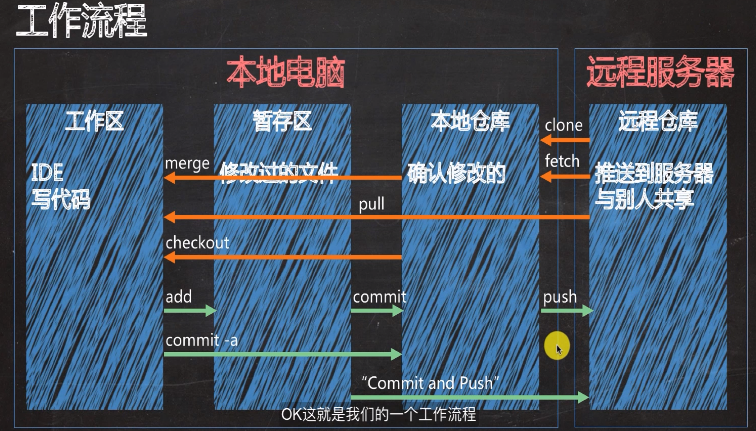
\includegraphics[width=0.9\textwidth]{pictures/git.png}
\caption{Git 工作流程\footnote{\url{https://www.bilibili.com/video/BV1mb411n7Nw?p=3}}}
%\label{fig:by:table}
\end{figure}

\begin{enumerate}
\item  主管人创建主远程仓库。
\item 协作人克隆主远程仓库,并拉取到本地。
\item 协作人在本地修改,上传到协作人的克隆远程仓库。
\item 协作人立即(或积累一定程度后),回到主远程仓库网页上,通过 Github 页面提交 pull requests。
\begin{itemize}
\item 首先,找到绿色的 New pull requests 按钮并点击,然后点击图中的 compare across forks;
\item 选择要提交的内容,通过比较文件差异,确认无误之后,点击绿色的eate pull request 即可。
\end{itemize}
\item 主管人在接到推送通知后,首先保证自己本地库与主远程仓库一致,否在合并时仍需回到这一步。
\item 主管人拉取协作人的远程仓库到本地,形成一个分支。
\item 主管人合并协作人的分支到主分支上。
\item 主管人再将合并后的最新版本推送到主远程仓库,至此完成一次协作。
\end{enumerate}
注意:无论是创始人还是协作人的远程仓库和本地库,都是相互独立的。


\subsection{创建远程仓库}
在相关网站上注册账户,并根据指示创建远程仓库。



\subsection{推送到远程仓库}
\url{https://www.bilibili.com/video/BV1pW411A7a5?p=35}
\begin{enumerate}
\item 添加远程仓库地址并设置别名:\verb|git remote add <name> <https://address> |,其中“name”为别名。
\item 查看远程仓库:\verb|git remote -v|。
\item 推送分支:\verb|git push <name> <branch>|,其中“name”为远程仓库别名,“branch”为要推送分支的名称,一般为主分支“master”。第一次推送还需要参数:\verb|-u|。
\begin{itemize}
\item 特别注意: 当在网页上创建远程仓库的时候,如果勾选了相关初始文件选项,那么直接推送时会报错,如\\
“failed to push some refs to https://github.com/guyibang/TEST2.git”\\
这是由于新创建的远程仓库中的初始文件不在本地仓库目录中。
\item 这时需要先进行合并再推送,即:\verb|git pull --rebase <name> <branch>|。
\item 如果具有不同的提交历史,则需进行强制合并:\\ 
\verb|git pull <name> <branch> --allow-unrelated-histories |
\end{itemize}
\end{enumerate}




\subsection{SSH免密推送设置}




\subsection{拉取和获取远程仓库}
\begin{itemize}
\item git pull:从远程仓库拉取最新版本到本地,并自动合并。
\item git fetch:从远程仓库获取最新版本到本地,但不会自动合并。
\end{itemize}


\subsection{主分支合并}
例如:
\begin{itemize}
\item[Step 1:] From your project repository, check out a new branch and test the changes.
\begin{enumerate}
\item git checkout -b Limingtan11-master master

\item git pull https://github.com/Limingtan11/SiSR.git master
\end{enumerate}

\item [Step 2:] Merge the changes and update on GitHub.
\begin{enumerate}
\item  git checkout master

\item git merge --no-ff Limingtan11-master

\item git push origin master
\end{enumerate}
\end{itemize}



\subsection{邀请合作者}
\begin{enumerate}
\item 进入自己的远程仓库主页,点击“Settings”;
\item 点击左侧“Options”栏目下的“Manage access”;
\item 就可以用“用户名”、“邮箱”等形式邀请了。
\end{enumerate}













\chapter{\LaTeX{}——编译型文档排版系统}
\section{学习参考资料}
\begin{itemize}
\item 安装: 啸行,一份简短的关于\LaTeX{}安装的介绍,\url{https://github.com/OsbertWang/install-latex}
\item 介绍:\url{http://mirror.utexas.edu/ctan/info/lshort/chinese/lshort-zh-cn.pdf}
\item 指南:\url{https://www.tug.org/texlive/doc/texlive-zh-cn/texlive-zh-cn.pdf}
\end{itemize}


\section{基本思想和历史}
我觉得它与Word的最大不同,应该是输入的方式了。它是靠直接“说”来代替Word中的那些不断缓慢的操作。比如:Word中改变字的颜色,是靠操作来完成的,选则相应的文字,然后去点击一些操作图标。而它是在要改变颜色的那段直接写上“换成某某颜色”的命令。这样书写公式就很简单,它可以像我们读公式一样,直接输上去就行了。比如$\sqrt{2}$,它可以直接输类似“根号2”的命令,即:\verb|$\sqrt{2}$|。也就是说一切操作只靠键盘就可以完成,甚至鼠标都不用点。这样是极大提高工作效率。对于那些老手来说,一路敲过去,转换出来就是漂亮的排版了。这样输公式爽多了。但要记住一堆命令。初学起来就不习惯了。

但是我觉得这还是个历史产物。以后随着技术不断先进,手写功能越来越强大,将是与手写识别相结合的情况。直接手写输入公式,就可以转换成自己想要的效果。对于一些微调又可以用命令来做。

\rightline{——冷轩\qquad}



\section{主体发行版——\TeX{} Live }
\subsection{Win10下安装}
注意要点:
\begin{itemize}
\item 全部安装占用空间比较大,。。。
\item 手动添加编译器路径到路径环境变量:
This PC->Advanced system settings->Advanced->Environment Variables...(右下角)->System variables->Path,点开。添加C:/texlive/2020/bin/win32。大家安装的路径可能不一样,但是选择\LaTeX{}相关编译器的路径就行。要点是,一定是编译器所在路径,上一级都不行。
\end{itemize}



\subsection{Ubuntu下安装}
(1)下载镜像
直接下载DVD光盘镜像的。不建议网络安装。官网主页:\url{http://www.tug.org/texlive/}


(2)安装
\paragraph{(a)文字界面安装}
%安装过程我没用图形界面,因为图形界面还要先安装一个包,觉得麻烦。
文字界面也简单,在终端中运行 Perl 脚本install-tl。 这就是在终端中运行一个文件。 运行一个文件, 当然需要告诉电脑文件在哪里了,于是在终端输入该脚本的全路径就行了,如:\\
\verb*|perl /home/phileas/texlive/install-tl|\\
或先转到相应的目录下,再执行,如:\\
\verb*|cd /home/phileas/texlive|\\
\verb*|perl install-tl|

运行后,会出现各种选项和提示。可以看到,texlive是装在文件系统中的,你可以更改安装的路径,或开启终端中的超级用户的权限,再来运行这个脚本。开启超级用户权限的方法是:在终端中输入命令:sudo -i。这样就可以安装了。

\paragraph{(b)图形界面安装}
建议使用图形安装界面,因为宏包用图形界面管理很方便,过程如下:
\begin{enumerate}
\item \verb*|sudo -i| 开启超级用户权限,这是因为默认安装到文件系统中,而改动文件系统是需要超级用户权限的,也可以不开启,到时选个可以安装的路径就行了。
\item  \verb*|apt-get install perl-tk| 安装 perl-tk 包才能用图形安装界面
\item 挂载镜像\\
先将光盘镜像挂载到一个文件夹中,如:/home/phileas/texlive,意思是:根目录/下的home文件夹phileas中的texlive文件夹。先找出光盘镜像的全路径,很简单,选中你的光盘镜像右键属性中有写,这个路径或许当你拷贝进这个文件时你就已经知道了,我放的位置是,\\
/home/phileas/desktop/texlive2011-20110705.iso,
最后一项是该文件名。挂载方法是在终端中,敲命令:\\
sudo mount /home/phileas/Desktop/texlive2011-20110705.iso/~~ /home/phileas/texlive ,
注意两个路径之间有空格。这样就挂载好了。(注意路径区分大小写)
\item cd挂载的镜像文件夹下,终端输入perl install-tl  - -gui
\item 有些选项,自己看着办。注意勾选建立符号链接(symbol link),很简单,勾选上就有了,不建立这个,之后在终端开启图形管理宏包界面的命令tlmgr - - gui就会报错说没有这个命令,其实还是要再加链接。所以这里记得勾选。(安装时没勾选也没关系,这部分内容在texlive相应版本的说明文档中说的很清楚。)
\item 点击安装

\item 如果安装时忘了勾选符号链接,则需添加环境变量。在\verb|~/.bashrc|文件中添加\\
\verb|export PATH=$PATH:/usr/local/texlive/2018/bin/x86_64-linux|\\
\verb|export MANPATH=$MANPATH:/usr/local/texlive/2018/texmf-dist/doc/man|\\
\verb|export INFOPATH=$INFOPATH:/usr/local/texlive/2018/texmf-dist/doc/info|\\
然后在终端中使环境变量生效:\\
\verb|source ~/.bashrc|

\item 调出图形管理宏包界面,在终端输入tlmgr - -gui,这时要改宏包更新源,在option选项改成网络为默认更新源。不然还是更新不了。
\end{enumerate}


\subsection{MacOS下安装}
\begin{itemize}
\item 命令行下安装 HomeBrew, 主页是:\url{https://brew.sh/}
\item 安装 MacTex, 命令行下使用 \emph{brew cask install mactex} 安装, 参考: \url{https://formulae.brew.sh/cask/mactex}
\item 选择一个写 \LaTeX{} 的文本编辑器,比如 Emacs、Sublime、VS Code
\end{itemize}

\section{Texworks}
注意:有时候Texworks没有自动找到\LaTeX{}相关编译器的路径。这时需要手动添加
Edit->Perference->Tyepsetting,添加
C:/texlive/2020/bin/win32(win10系统)。要点是,一定要是编译器所在目录,上一级都不行。


\subsection{安装}
官网:\url{https://www.tug.org/texworks/}\\
\verb|sudo add-apt-repository ppa:texworks/stable|\\
\verb|sudo apt-get update|\\
\verb|sudo apt-get install texworks|


\subsection{简述}
[转] \url{http://blog.sina.com.cn/s/blog_630306a50101fjwy.html}

Texworks 是目前我用的最多的\LaTeX 编辑软件,不是跟 ddswhu 交流,我还一直不知道,里面还蕴含着很多方便快捷的缩写。这里就是主要谈谈这些快捷缩写。这些缩写都在一个叫completion 的文件中,到 Texworks 安装目录下找找。

首先,对 TeXworks 的自动补全功能解释一下:

1、在 TeXworks 的编辑窗里面键入 xa,按下tab,出现了 \verb|\alpha|,这就是最简单的补全,对简单命令的补全。

2、在 TeXworks 键入usep,按下tab建,得到了 \verb|\usepackage{}|,这就是最普通的补全,给出命令后的必须参数括号,并且光标停留在括号内。

3、在TeXworks键入usepo,按下tab,得到了 \verb|\usepackage[]{•}|,这是对含有可选参数的命令的补全,光标停在可选参数的中括号内,当我们把可选参数补完之后,按下ctrl+tab组合键,光标进入后面的必需参数括号内(后面的位置称为placeholder)。其中ctrl+tab是移向往下最接近的一个placeholder,shift+tab是移向往上最近的一个placeholder。
 
在刚才的例子中,我们只按了一次tab,假如我们键入的引导词是若干个命令的引导词的前部分,则继续按下tab键会在这几个命令中切换,得到你想要的命令。
 
好了,为了使用自动补全,我们需要记住引导词。在TeXworks中,已经定义了很多的引导词,而且也允许用户自己定义新的引导词。
 
下面对常用的引导词归类。
 
\subsection{环境类}
对于环境的补全,引导词第一个字母均为b,后面字母个数不定,但是,对绝大多数的环境,只需要使用环境名的前三个字母就行,即为"b+xyz+[tab]"。
 
比如 itemize 环境,根据规则,我们需要键入 "bite",然后按下tab键,即得到了
\begin{verbatim}
\begin{itemize}
\item
 
\end{itemize}•	
\end{verbatim}

符合此规则的环境有document,abstract,align,tabular,appendix,bmatrix,pmatrix,cases,
description,center,equation,enumerate,eqnarray,figure,flalign,
gather,item,letter,list,minipage,multiline,picture,split,subequations,
theorem,titlepage,trivlist,varwidth,verbatim,等。
 
注意事项:如果环境名开头带有the,则xyz为除去the之后的环境名的前三个字母。比如bind=theindex环境、bbib=thebibliography环境。
 
另外需要注意的是:星号环境在原来引导词后加s,即为"b+xyz+s+[tab]",如果环境有可选项,需要使用可选项,则需要在末尾加上o(option的意思),即为"b+xyz+o+[tab]"。
 
几个特殊的环境:

align    :b+ali(s)
alignat   :b+ali+at(s)
aligned  :b+ali+ed
alignedat :b+ali+edat(o)
 
verbatim  :bver
verse    :bvers
tabular   :b+tab
tabularx  :b+tabx
tabbing  :b+tabb
table    :b+tabl、b+tbl (s,o,so)
 
居左、居右环境、居中
flushleft+flushright :b+fl+l/r
\verb|\centering|         : cen
 
 
 
 \subsection{字体}
(1)普通字体命令

(1.1)\verb|\textbf, \texttt, \textsf, \textsc, \textsl, \textit, \textup|

   方法一、由字体属性的两个关键字构成,比如 sc+[tab键],textit有问题,em表示\verb|\emph{}|
   
   方法二、\verb|\text(b/t/s/i/w...)+[tab键]|
   
   注意:\verb|\textwidth| 也是 \verb|\textw|

(1.2)属性的第二种表示方式、"属性关键字+d"

    bfd: \verb|\bfseries|
    ttd: \verb|\ttfamily|
    sfd: \verb|\sffamily|
    scd: \verb|\scshape|
    sld:  \verb|\slshape|
    itd:  \verb|\itshape|
    upd: \verb|\upshape|
    emd: \verb|\em|
 
(2)数学字体命令:
    
  \verb|\mathbf, \mathrm, \mathcal, \mathsf, \mathtt, \mattit|
  
    引导词为"m+字体属性关键字"。比如:mbf\verb|\mcal|
 

 
 \subsection{希腊字母类}
方法:”x+[c(大写符号)]+符号首字母”

适用的字母有:
\begin{verbatim}
\alpha, \beta , \chi, \delta, \gamma, \Gamma, \iota, \mu, \lambada,
\Lambda, \mu, \nu, \omega, \Omega, \pi, \sigma, \zeta, \rho, \tau,
\upsilon, \xi, \Xi
\end{verbatim}

注意以下相同首字母的写法(特殊):

\verb|\epsilon|: x+e
\verb|\varepsilon|: x+v+e
\verb|\eta|: x+et
\verb|\phi| :x+p
\verb|\varphi| :x+v+p
\verb|\phi| :x+ph
\verb|\Phi| :x+c+ph
\verb|\varphi| :x+v+ph
\verb|\psi| :x+ps
\verb|\Psi| :x+c+ps
\verb|\tau| :x+t
\verb|\theta| :x+th
 
 
 
 \subsection{章节命令}
cha     =\verb|\chapter{}|

sec(o)   =\verb|\section{}|

ssec(o)  =\verb|\subsection{}|

sssec(o) =\verb|\subsubsection{}|

 
\subsection{参考文献}
bbib      =\verb|\begin{thebibliography}|
bibitem   =\verb|\bibitem|
bibitemo  =\verb|\bibitem[]|
bibstyle   =\verb|\bibliographystyle{}|
biblio     =\verb|\bibliography{}|
 
  
 \subsection{杂项与普通命令}
1、括号

dd : \verb|\( \)|

\verb|d+希腊字母表达式=\(希腊字母\)|

例如:dxa = \verb|\(\alpha\)|
 
2、普通命令

usep   =\verb|\usepackage{}|

foot    =\verb|footnote foot|

frac    =\verb|\frac|

fbox   =\verb|\fbox|

fboxo  =\verb|\framebox|

href   =\verb|\href|

incg   =\verb|\includegraphics{}|

incgo  =\verb|\includegraphics[]{•}|

ncol(newcolumn) = \verb|&|

newc  =\verb|\newcommand{}{•}|

newe  =\verb|\newenvironment{}{•}{•}|

newpg =\verb|\newpage|

pgref  =\verb|\pageref{}|

pgs   =\verb|\pagestyle{}|

sqrt   =\verb|\sqrt{}|

toc   =\verb|\tableofcontents|

listf   =\verb|\listoffigures|

list   =\verb|\listoftables|
multic =\verb|\multicolumn{}{•}{•}|



%\section{Sublime Text}




\chapter{科研入门技能及心得}
\section{科研导师的选择}
\begin{enumerate}
\item 必须步骤:人品和性格匹配调查,可靠来源为现任组里成员,最好为新老成员。
\end{enumerate}



\section{一些该注册的}
\subsection{Gmail}
 至少申请两个,一个注册用,一个通讯用(真名)。

\begin{itemize}
\item Gmail查看所有未读邮件\footnote{\url{https://jingyan.baidu.com/article/cbcede0761144902f40b4d18.html}}:
\begin{enumerate}
\item 打开登陆Gmail网页,在主界面点击上面的搜索框的下拉选项;
\item 弹出下拉窗口,在第一行点击搜索所有邮件,然后在下拉选项中选择未读邮件,只搜索未读邮件;
\item 然后日期范围选最大的,选一年,然后点击搜索,意思就是搜索一年内所有未读邮件。
\end{enumerate}
或者
\begin{enumerate}
\item 打开Gmail网页,在搜索框中输入代码“is:unread ”
\end{enumerate}
\end{itemize}



\subsection{Google Scholar}


\subsection{Research gate}


\subsection{OCRC}




\section{文献管理、检索与推送}
文献是科研之魂,高效管理文献是科研的第一步——冷轩 \quad 语 (这里的文献特指期刊论文)
\subsection{文献管理的基本思想}
\begin{itemize}
\item 平等的看待每一篇文献。不需要专门的、特别的去存储某些文献。文献的时效性太短了,发现多年前的Nature、Science 正刊等对现在没有任何参考意义。

\item 文献多元分类。每篇文献有不同的标签。

\item 文献不同平台、设备的同步。常见的应用场景是,工作电脑下载了文献,然后用带手写笔的设备去细看、标记。
\end{itemize}
仅仅靠本地创建文件夹的方式去管理,是非常不方便的。需要采用专业的文献管理软件,非常推荐Zotero。





\subsection{免费文献管理工具——Zotero}
参考资料:
\begin{itemize}
\item 青柠学术微信公众号的专辑“Zotero|打造最佳文献生态”(由于网络链接比较繁杂,请自行搜索)
\item \url{https://zhuanlan.zhihu.com/p/28325366}
\end{itemize}


Zotero (\url{https://www.zotero.org/}) 是一款免费、跨平台并且强大的文献管理工具,如图(\ref{fig566})所示。
\begin{figure}[h!]
\centering
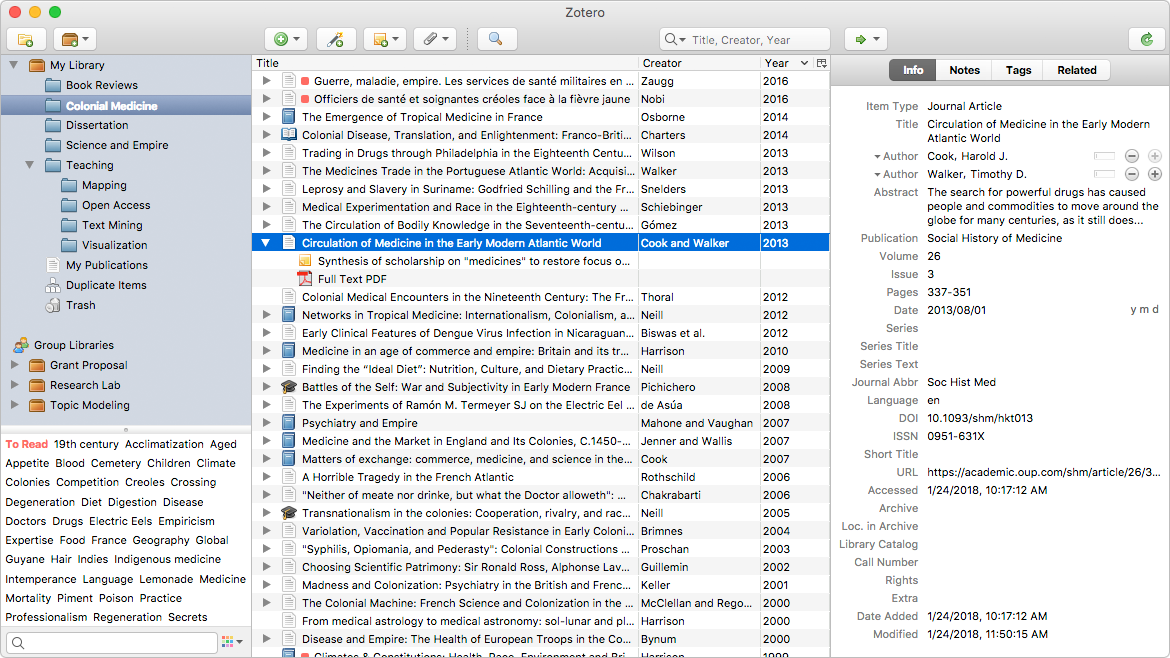
\includegraphics[width=0.8\textwidth]{pictures/zotero.png}
\caption{Zotero基本界面}
\label{fig566}
\end{figure}




\paragraph{(1)常用的功能}
如图(\ref{fig566})所示,Zotero基本分成三栏,左边是分类区,中间是文献区,右边是文献详细信息区。
分类区又分为上下两区,上面称为 Collection,下面则是每篇文献的标签汇总称为Tag。
\begin{itemize}
\item 前往官网下载安装相应版本和插件,并注册帐号。
\item 在 Library 创建 Collection。
\item 选中 Collection 就可以在程序中间文献区导入文献,这样 Zotero 就自动获取文献名、作者、年份等信息。导入文献有两种方式:
\begin{itemize}
\item Link to File: 这种是建立与本地文献链接,不上传到云盘模式。
\item Store Copy of File: 这种是复制到Zotero存贮区上传到云盘模式。请参考多平台、多设备同步。
\end{itemize}
\item 选择一篇文献,在右侧Tags处写上标签,一般多个,如:特别关注的作者、文献中的方法和研究对象。
\item 所有标签就会出现在 第一栏下面区域。首先在 Collection 区域选择 Library,中栏就能呈现所有文献,再在 Tag 区域选中任意标签,就会在中栏筛选出相应的标签。选中多个标签,则是取文献的交集。
\item 通过标签解决了一篇文献多个分类的问题。
\item Collection 中的文献复制有两种方式:
\begin{itemize}
\item 选中 + 拖放:在多个Colletion中复制并保留文献条目; 
\item 选中 + shift + 拖放:从不同Colletion中移动条目。
\end{itemize}
\end{itemize}



\paragraph{(2)文献快速下载与导入}
通过相关的浏览器插件,可以一步实现文献下载和Zotero的导入。但是前提的有,1)Zotero是打开着的;2)自己有文献下载的权限,能把文献下载下来,如果不能,则只会保存一个文献信息,需要后期关联。



\paragraph{(3)多平台、多设备同步}
这是一个非常实用的功能。

\emph{以我为例,主要工作系统是 Ubuntu 系统。但为了实现无纸化办公,我喜欢用微软的 Surface 来阅读文献。而且用 Surface 的笔可以直接在pdf文献上标注,标注也可以同步到主要工作电脑上,非常方便。}

Zotero 自己是有空间同步本地文献的,但是价格太贵。主要可以采用两种方式:1)Zotero +同步盘(任意云盘,软链接);2)Zotero +坚果云WebDAV。推荐后者,详情请参考青柠学术微信公众号专辑,Zotero|打造最佳文献生态。

\paragraph{(4)文献全文检索并自动更新}
还是参考青柠学术Zotero专辑。在“My library”右键有“New Saved Search”。这个可以对文献库中文献进行特定检索,并随着加入的文献自动更新。



\subsection{文献下载}
\begin{itemize}
\item \url{https://bookos-z1.org/}:英文专业书籍下载网站
\item \url{sci-hub.tw}:文献下载网站
\item Zotero + Zotero Connector + Zotero-shortdoi + SCi-Hub: 文献下载标签一条龙,几乎能完成99\%文献下载,参考青柠学术的Zotero专题。
\end{itemize}


\subsection{文献检索与推送——Google学术}
参考:\url{https://scholar.google.com/intl/en/scholar/help.html#overview}



\subsection{Pdf批量全文搜索工具——Recoll}
\begin{itemize}
\item Recoll 网址:\url{https://www.lesbonscomptes.com/recoll/}

\item 参考网址:\url{http://www.linuxdown.net/install/faq/20160318_how_linux_5065.html}
\end{itemize}





\section{自然科学论文写作}
\subsection{摘要(Abstract)}
摘要一般5到6句话。
\begin{itemize}
\item 第一句:大背景;
\item 第二句:领域中有什么问题、我想做什么、有什么是未知的、有什么需要做的;
\item 有些文章不写第一句、第二句
\item 第三句:我用什么方法研究了什么东西;
\item 第四、五句:有什么结果。或加一句分析一下;
\item 最后一句:意义(重要性)。
\end{itemize}


\subsection{引言(Introduction)}
引言的写作直接影响到读者对文章进一步了解的兴趣, 建议包括以下内容\footnote{参考自物理学报的投稿模板}:
\begin{enumerate}
\item 本研究领域背景的综述;
\item 其他学者已有研究成果的详细描述;
\item 陈述为什么需要进行更多的或进一步的研究;
\item 阐述作者本项研究的目的和创新性;
\item 简述本文开展的研究工作;
\item 本项研究结果的意义(可选项)。
\item 特别指出的是, 希望在引言部分介绍和引用国内外期刊中本研究领域的最新研究成果, 以帮助读者清楚了解该领域的最新进展及本文的创新点。
\end{enumerate}



\section{演示文稿(PPT)制作}
图和列表(关键词)



\section{墙报制作}




\section{科研资源}
\subsection{光学相关}
 \begin{itemize}
\item \url{http://toolbox.lightcon.com/}
\end{itemize}









\part{Ubuntu}
\include{chapters/Ubuntu}

\part{Linux}
\include{chapters/Linux_foundation}
\include{chapters/Linux_command}
\chapter{Shell \& Shell Script}
Shell的学习与Linux的学习是密切相关的,要学Linux必须学Shell。
\section{什么是Shell}
Shell 是用户用来控制计算机的一个接口。与现代普通用户常见的计算机操作界面——图形化界面不同的是,这里指的是纯文字界面,称为命令行界面。只要能够操作应用程序的接口都能够称为壳程序。狭义的壳程序指的是命令行界面的软件,如常见的 bash 等。 广义的壳程序则是图形接口的软件,因为图形接口其实也是操作各种应用程序来调用核心工作。命令行界面控制计算机高效、稳定、准确,适合程序员用户。

Shell程序的出现是跟操作系统设计思想密切相关的。对于Linux系统,管理整个计算机硬件的是操作系统的核心 (Kernel),这个核心是需要被保护。因为操作系统其实是一组软件,只不过这组软件控制着整个硬件与管理系统的活动监测。 如果这组软件能被用户随意的操作,若使用者应用不当,将会使得整个系统崩溃。因为操作系统管理的就是整个硬件功能! 所以不能够随便被一些没有管理能力的终端用户随意使用。

但是我们总是需要让用户操作系统的,所以就有了在操作系统上面发展的应用程序。用户可以透过应
用程序来指挥核心, 让核心达成我们所需要的硬件任务。应用程序是在最外层的,就如同鸡蛋的外壳一样,所以被称为壳程序 (Shell) 。通过Shell可以调用其他独立的应用程序,即通过Shell来操作其他应用程序来指挥核心完成工作,所以说Shell 是用户用来控制计算机的一个接口。用户通过Shell将指令传递给Kernel,Kernel再来控制硬件完成工作。



\section{常见的Shell}
简单点理解,Shell就是系统跟计算机硬件交互时使用的中间介质,它只是系统的一个工具。实际上,在Shell和计算机硬件之间还有一层东西那就是系统内核了。打个比方,如果把计算机硬件比作一个人的躯体,而系统内核则是人的大脑,至于Shell,把它比作人的五官似乎更加贴切些。回到计算机上来,用户直接面对的不是计算机硬件而是Shell,用户把指令告诉Shell,然后Shell再传输给系统内核,接着内核再去支配计算机硬件去执行各种操作。

Shell是一种脚本语言,那么,就必须有解释器来执行这些脚本。Unix/Linux上常见的Shell脚本解释器有bash、sh、csh、ksh等,习惯上把它们称作一种Shell。我们常说有多少种Shell,其实说的是Shell脚本解释器。
\begin{itemize}
\item bash

bash是Linux标准默认的Shell,本教程也基于bash讲解。bash由Brian Fox和Chet Ramey共同完成,是BourneAgain Shell的缩写,内部命令一共有40个。它基于Bourne shell,吸收了C shell和Korn shell的一些特性。bash完全兼容sh,也就是说,用sh写的脚本可以不加修改的在bash中执行。

\item sh

sh 由Steve Bourne开发,是Bourne Shell的缩写,sh 是Unix 标准默认的Shell。

\item ash

ash shell 是由Kenneth Almquist编写的,Linux中占用系统资源最少的一个小Shell,它只包含24个内部命令,因而使用起来很不方便。

\item csh

csh 是Linux比较大的内核,它由以William Joy为代表的共计47位作者编成,共有52个内部命令。该Shell其实是指向/bin/tcsh这样的一个Shell,也就是说,csh其实就是tcsh。

\item ksh

ksh 是Korn shell的缩写,由Eric Gisin编写,共有42条内部命令。该Shell最大的优点是几乎和商业发行版的ksh完全兼容,这样就可以在不用花钱购买商业版本的情况下尝试商业版本的性能了。
\end{itemize}



\section{Shell的特性}
\begin{itemize}
\item \textbf{记录命令历史}

\qquad 我们敲过的命令,Linux 是会有记录的,预设可以记录1000条历史命令。这些命令保存在用户的 home 目录中的  .bash\_history 文件中。有一点需要知道的是,只有当用户正常退出当前 Shell 时,在当前 Shell 中运行的命令才会保存至  .bash\_history 文件中。

\qquad 与命令历史有关的有一个有意思的字符那就是``!''了。常用的有这么几个应用:

(1)!! (连续两``!''),表示执行上一条指令;

(2)!n(这里的n是数字),表示执行命令历史中第n条指令,例如``!100''表示执行命令历史中第100个命令;

(3)!字符串(字符串大于等于1),例如,!ta,表示执行命令历史中最近一次以ta为开头的指令。

\item \textbf{命令和文件名补全}

\qquad 按tab键,它可以帮你补全一个指令,也可以帮你补全一个路径或者一个文件名。连续按两次tab键,系统则会把所有的指令或者文件名都列出来。

(1)tab 接在一串命令的第一个字的后面为命令补全;

(2)tab 接在一串命令的第二个字以后面则为文件或路径补全。

\item \textbf{命令别名配置功能——alias}

\qquad 输入 alias会看到目前系统预设的命令别名有哪些。自定义别名形如:

\verb|alias lm='ls -al'|

这样lm 会等于 ls -al 这样的一个功能,即显示这个目录底下的所有文件 (包含隐藏档) 及所有的文件属性。
这个就是bash所特有的功能之一了。我们可以通过alias把一个常用的并且很长的指令别名一个简洁易记的指令。如果不想用了,还可以用unalias解除别名功能。需要注意的是命令的别名在Shell注销后就会失效,如果要保留,就得写入Shell的配置文件。

\item \textbf{通配符}

\qquad 除了完整的字符串之外, bash 还支持许多的通配符来帮助用户查询与命令下达。 举例来说,想要知道 /usr/bin 底下有多少以 X 为开头的文件吗?使用:ls -l /usr/bin/X* 就能够知道。此外,还有其他可供利用的通配符, 这些都能够加快使用者的操作。
\end{itemize}



\section{Bash Shell的内建命令}
 为了方便 Shell 的操作, Bash 内建了很多命令。对于如何知道命令是外部命令还是内建在Bash当中,可以利用type命令,其格式如下:
 
 \verb|type [-tpa] name|

选项与参数:
\begin{itemize}
\item 不加任何选项与参数时,type 会显示出 name 是外部命令还是 Bash 内建命令;
\item -t:当加入 -t 参数时,type 会将 name 以底下这些字眼显示出它的意义:
	\begin{itemize}
	\item  file    :表示为外部命令;
       \item alias   :表示该命令为命令别名所配置的名称;
      \item builtin :表示该命令为 bash 内建的命令功能。
	\end{itemize}
\item -p  :如果后面接的 name 为外部命令时,才会显示完整文件名;
\item -a  :会由 PATH 变量定义的路径中,将所有含 name 的命令都列出来,包含 alias。	
\end{itemize}



\section{Bash的进站与欢迎信息}
在终端机接口 (tty1$\sim$tty6) 登陆的时候,会有几行提示的字符串,那就是进站画面。这些字符串存储在/etc/issue文件里面。例如,
\begin{lstlisting}[language=sh]
xuan@x:~$ cat /etc/issue
Ubuntu 14.04.2 LTS \n \l

xuan@x~$ 
\end{lstlisting}

issue 内的各代码意义

\verb|\d| 本地端时间的日期;

\verb|\l| 显示第几个终端机接口;

\verb|\m| 显示硬件的等级 (i386/i486/i586/i686...);

\verb|\n |显示主机的网络名称;

\verb|\o |显示 domain name;

\verb|\r |操作系统的版本 (相当于 uname -r)

\verb|\t |显示本地端时间的时间;

\verb|\s |操作系统的名称;

\verb|\v |操作系统的版本。




\section{Shell的配置文件}
\subsection{login与non-login Shell}
login Shell与non-login Shell的区别在于有没有login:
\begin{itemize}
\item login shell:取得 bash 时需要完整的登陆流程的,就称为 login shell。举例来说,由 tty1$\sim$tty6 登陆,需要输入用户的账号与密码,此时取得的 bash 就称为“ login shell ”;

\item non-login shell:取得 bash 接口的方法不需要重复登陆的举动,举例来说,

\qquad(1)以 X window 登陆 Linux 后, 再以 X 的图形化接口启动终端机,此时那个终端接口并没有需要再次的输入账号与密码,那个 bash的环境就称为 “non-login shell”。

\qquad (2)在原本的 bash环境下再次调用 bash 这个命令,同样的也没有输入账号密码, 那第二个 bash (子程序) 也是 “non-login shell” 。
\end{itemize}

在这两种取得bash的情况中,bash读取的配置文件不一样。一般说来,login Shell读取的配置文件是:
\begin{itemize}
\item \verb|/etc/profile|:这是系统整体的配置,最好不要修改这个文件;

\item \verb|~/.bash_profile| 或 \verb|~/.bash_login| 或 \verb|~/.profile|:属于用户个人配置文件,要改自己的数据,就写入这里。
\end{itemize}


\subsection{/etc/profile}
/etc/profile,login Shell读取的配置文件。这个配置文件可以利用用户ID (UID) 来决定很多重要的变量数据, 这也是每个用户login取得 bash 时一定会读取的配置文件。 所以如果想要帮所有用户配置整体环境,那就是修改这里。不过,没事还是不要随便改这个文件。这个文件配置的变量主要有:
\begin{itemize}
\item PATH:会依据 UID 决定 PATH 变量要不要含有 sbin 的系统命令目录;
\item MAIL:依据账号配置好使用者的 mailbox 到 /var/spool/mail/账号名;
\item USER:根据用户的账号配置此一变量内容;
\item HOSTNAME:依据主机的 hostname 命令决定此一变量内容;
\item HISTSIZE:历史命令记录笔数。
\end{itemize}

/etc/profile 还会调用外部的配置文件,如:/etc/profile.d/*.sh,即只要用户具有r的权限,那么在 /etc/profile.d/ 这个目录内且扩展名为 .sh的文件就会被 /etc/profile调用。如果需要帮所有用户配置一些共享的命令别名时, 可以在这个目录底下自行创建扩展名为 .sh 的文件,并将所需要的数据写入即可。这样的机制让我们的 bash 操作接口变的非常友善。


\subsection{$\sim$/.bash\_profile、$\sim$/.bash\_login和$\sim$/.profile}
对于login Shell,bash 在读完了整体环境配置的 /etc/profile 并藉此调用其他配置文件后,接下来则是会读取用户的个人配置文件。 在 login shell 的 bash 环境中,所读取的个人偏好配置文件主要有三个,依序分别是:
\begin{enumerate}
\item \verb|~/.bash_profile|
\item \verb|~/.bash_login|
\item \verb|~/.profile|
\end{enumerate}

其实 bash 的 login shell 配置只会读取上面三个文件的其中一个, 而读取的顺序则是依照上面的顺序。也就是说,如果 \verb|~/.bash_profile|存在,那么其他两个文件不论有无存在,都不会被读取。 如果 \verb|~/.bash_profile|不存在才会去读取 \verb|~/.bash_login|,而前两者都不存在才会读取 \verb|~/.profile| 的意思。 会有这么多的文件,其实是因应其他 shell 转换过来的使用者的习惯而已。


\subsection{$\sim$/.bashrc}
当取得 non-login shell 时,该 bash 配置文件仅会读取 \verb|~/.bashrc| 而已!


\subsection{其他相关配置文件}
还有一些配置文件可能会影响到bash 操作的:
\begin{itemize}
\item \verb|~/.bash_history|

\qquad 默认情况下, 我们的历史命令就记录在这里。而这个文件能够记录几笔数据,则与 HISTFILESIZE 这个变量有关啊。每次登陆 bash 后,bash 会先读取这个文件,将所有的历史命令读入内存, 因此,当我们登陆 bash 后就可以查知上次使用过哪些命令。

\item \verb|~/.bash_logout|

\qquad 这个文件则记录了,当我注销 bash 后,系统再帮我做完什么动作后才离开,的意思。 可以去读取一下这个文件的内容,默认的情况下,注销时, bash 只是帮我们清掉屏幕的信息而已。 不过,我们也可以将一些备份或者是其他认为重要的工作写在这个文件中 (例如清空缓存盘), 那么当我们离开 Linux 的时候,就可以解决一些烦人的事情。

\item \verb|/etc/man.config|

\qquad 这个文件乍看之下好像跟 bash 没相关性,但是对于系统管理员来说, 却也是很重要的一个文件。这个文件的内容规范了使用 man 的时候, man page 的路径到哪里去寻找。所以说的简单一点,这个文件规定使用 man命令的时候,该去哪里查看数据的路径配置。

\qquad 那么什么时候要来修改这个文件呢?如果是以 tarball 的方式来安装数据,那么 man page 可能会放置在 /usr/local/softpackage/man 里头,那个 softpackage 是软件名称, 这个时候就得以手动的方式将该路径加到 /etc/man.config 里头,否则使用 man 的时候就会找不到相关的说明档。

\qquad 事实上,这个文件内最重要的其实是 MANPATH 这个变量配置。 我们搜寻 man page 时,会依据 MANPATH 的路径去分别搜寻。另外,要注意的是, 这个文件在各大不同版本 Linux distributions 中,名称都不太相同,例如 CentOS 用的是 /etc/man.config ,而 SuSE 用的则是 /etc/manpath.config , 可以利用 [tab] 按键来进行文件名的补齐。
\end{itemize}


\section{通配符与特殊符号}
在 bash 的操作环境中还有一个非常有用的功能,那就是通配符 (wildcard) ,利用 bash 处理数据就更方便了。底下列出一些常用的通配符:
\begin{itemize}
\item \verb|*|:代表 “0 个到无穷多个”任意字符;

\item \verb|?|:代表“一定有一个”任意字符;

\item \verb|[ ]|:同样代表“一定有一个在括号内”的字符(非任意字符)。例如 [abcd] 代表“一定有一个字符, 可能是 a、b、 c、 d 这四个任何一个”;再说个例子\verb|*[0]|和\verb|*[0]*|,前者是寻找结尾为0的任意文件,后者则是寻找包含0的任意文件,把各自符号的意义套入就能分析出来;

\item \verb|[ - ]|:若有减号在中括号内时,代表“在编码顺序内的所有字符”。例如 [0-9] 代表 0 到 9 之间的所有数字,因为数字的语系编码是连续的;

\item \verb|[^ ]|:若中括号内的第一个字符为指数符号 “\verb|^|” ,那表示“反向选择”,例如 \verb|[^abc]| 代表 一定有一个字符,只要是非 a、 b、 c 的其他字符就接受的意思。
\end{itemize}

下面列出的则是bash 环境中的特殊符号:
\begin{itemize}
\item \verb|#|:批注符号,这个最常被使用在 script 当中,视为说明,在后的数据均不运行;
\item \verb|\|:跳脱符号,将“特殊字符或通配符”还原成一般字符;
\item\verb|||:	管线 (pipe),分隔两个管线命令的界定;
\item \verb|;|:连续命令下达分隔符,连续性命令的界定 (注意!与管道符并不相同);
\item \verb|~|:用户的家目录;
\item \verb|$|:取用变量前导符,亦即是变量之前需要加的变量取代值;
\item \verb|&|:工作控制 (job control),将命令变成背景下工作;
\item \verb|!|:逻辑运算意义上的“非” (not) 的意思;
\item \verb|/|:目录符号,路径分隔的符号;
\item \verb|>, >>|:数据流重导向,输出导向,分别是“取代”与“累加”;
\item \verb|<, <<|:数据流重导向,输入导向 ;
\item \verb|' '|:单引号,不具有变量置换的功能;
\item \verb|" "|	:具有变量置换的功能;
\item \verb|` `|	:两个“\verb|`| ”中间为可以先运行的命令,亦可使用 “\verb|$( )|”;
\item \verb|( )|	:在中间为子 shell 的起始与结束;
\item \verb|{ }|	:在中间为命令区块的组合。
\end{itemize}
所以文档名尽量不要使用到上述的字符。这里只是简单介绍,更详细的介绍参见相关章节。


\subsection{``~''后缀的文件}
当我们编辑文本文件时,保存后经常发现多了个后面带个``~''的同样名字的隐藏文件。这是前一个版本的系统自动备份的文件,万一发生错误和其他意外时,保留这些文件还是有一定作用的。如果觉得没必要,可以通过设置更改。

\begin{itemize}
\item
对于编辑器 gedit:编辑=>首选项=>编辑器,把保存文件时备份选项去掉就可以了;

\item
vim的话可以在其配置文件.vimrc中取消设置backup文件:\verb|set nobackup|。
\end{itemize}

\subsection{反斜杠}
因为命令太长, 于是可以就利用“\verb| \[Enter]| ”来将 [Enter] 这个按键“跳脱!”开来,让 [Enter] 按键不再具有“开始运行”的功能,好让命令可以继续在下一行输入。 需要特别留意, [Enter] 按键是紧接着反斜杠 (\verb|\|) 的,两者中间没有其他字符。 因为 \verb|\| 仅跳脱“紧接着的下一个字符”而已!所以,万一写成: \verb*|\ [Enter]|,亦即 [Enter] 与反斜杠中间有一个空格时,则 \verb|\| 跳脱的是“空格键”而不是 [Enter] 按键,这个地方请再仔细的看一遍!很重要!

如果顺利跳脱 [Enter] 后,下一行最前面就会主动出现 > 的符号, 就可以继续输入命令。也就是说,那个 > 是系统自动出现的,不需要输入。









\section{什么是Shell脚本}
% http://c.biancheng.net/cpp/shell/
计算机语言从执行过程的角度可以分为编译型语言和解释型语言(当然还有其他语言,如HTML、\LaTeX 标记语言等),但无论哪种语言,所有的语言编写出来的程序执行时要解释成计算机代码。
\begin{itemize}
\item 编译型语言:编写完程序后直接通过编译器转换程计算机代码生成可执行文件,以后每次执行时就不用进行转换,直接执行可执行文件即可。

很多传统的程序设计语言,例Fortran、Ada、Pascal、C、C++和Java,都是编译型语言。这类语言需要预先将我们写好的源代码(source code)转换成目标代码(object code),这个过程被称作“编译”。运行程序时,直接读取目标代码(object code)。由于编译后的目标代码(object code)非常接近计算机底层,因此执行效率很高,这是编译型语言的优点。但是,由于编译型语言多半运作于底层,所处理的是字节、整数、浮点数或是其他机器层级的对象,往往实现一个简单的功能需要大量复杂的代码。例如,在C++里,就很难进行“将一个目录里所有的文件复制到另一个目录中”之类的简单操作。

\item 解释型语言:编写完成后不用转换成计算机代码,而是在每次执行的时候再进行代码转换工作,脚本语言的好处是源文件能够直接进行修改,直接使用文本编辑器就能够打开。

解释型语言也被称作“脚本语言”。执行这类程序时,解释器(interpreter)需要读取我们编写的源代码(source code),并将其转换成目标代码(object code),再由计算机运行。因为每次执行程序都多了编译的过程,因此效率有所下降。使用脚本编程语言的好处是,它们多半运行在比编译型语言还高的层级,能够轻易处理文件与目录之类的对象;缺点是它们的效率通常不如编译型语言。不过权衡之下,通常使用脚本编程还是值得的:花一个小时写成的简单脚本,同样的功能用C或C++来编写实现,可能需要两天,而且一般来说,脚本执行的速度已经够快了,快到足以让人忽略它性能上的问题。脚本编程语言的例子有awk、Perl、Python、Ruby与Shell。
\end{itemize}

Shell本身是一个用C语言编写的程序,它是用户使用Unix/Linux的桥梁,用户的大部分工作都是通过Shell完成的。Shell既是一种命令语言,又是一种程序设计语言。作为命令语言,它交互式地解释和执行用户输入的命令;作为程序设计语言,它定义了各种变量和参数,并提供了许多在高级语言中才具有的控制结构,包括循环和分支。

它虽然不是Unix/Linux系统内核的一部分,但它调用了系统核心的大部分功能来执行程序、建立文件并以并行的方式协调各个程序的运行。因此,对于用户来说,Shell是最重要的实用程序,深入了解和熟练掌握Shell的特性极其使用方法,是用好Unix/Linux系统的关键。可以说,Shell使用的熟练程度反映了用户对Unix/Linux使用的熟练程度。

Shell有两种执行命令的方式:
\begin{itemize}
\item 交互式(Interactive):解释执行用户的命令,用户输入一条命令,Shell就解释执行一条。
\item 批处理(Batch):用户事先写一个Shell脚本(Script),其中有很多条命令,让Shell一次把这些命令执行完,而不必一条一条地敲命令。
\end{itemize}

Shell脚本和编程语言很相似,也有变量和流程控制语句,但Shell脚本是解释执行的,不需要编译,Shell程序从脚本中一行一行读取并执行这些命令,相当于一个用户把脚本中的命令一行一行敲到Shell提示符下执行。


说白了,Shell脚本就是一些命令的集合。举个例子,我想实现这样的操作:

1)进入到/tmp/目录;

2)列出当前目录中所有的文件名;

3)把所有当前的文件拷贝到/home/xuan目录下;

4)删除当前目录下所有的文件。

简单的4步在Shell窗口中需要你敲4次命令,按4次回车。这样是不是很麻烦?当然这4步操作非常简单,如果是更加复杂的命令设置需要几十次操作呢?那样的话一次一次敲键盘会很麻烦。所以不妨把所有的操作都记录到一个文档中,然后去调用文档中的命令,这样一步操作就可以完成。其实这个文档呢就是Shell脚本了,只是这个Shell脚本有它特殊的格式。

Shell脚本能帮助我们很方便的去管理服务器,因为我们可以指定一个任务计划定时去执行某一个Shell脚本实现我们想要需求。这对于Linux系统管理员来说是一件非常值得自豪的事情。现在的139邮箱很好用,发邮件的同时还可以发一条邮件通知的短信给用户,利用这点,我们就可以在我们的Linux服务器上部署监控的Shell脚本,比如网卡流量有异常了或者服务器web服务器停止了就可以发一封邮件给管理员,同时发送给管理员一个报警短信这样可以让我们及时的知道服务器出问题了。

有一个问题需要约定一下,凡是自定义的脚本建议放到/usr/local/sbin/目录下,这样做的目的是,一来可以更好的管理文档;二来以后接管你的管理员都知道自定义脚本放在哪里,方便维护。

Shell脚本通常都是以.sh 为后缀名的,这个并不是说不带.sh这个脚本就不能执行,只是大家的一个习惯而已。所以,以后你发现了.sh为后缀的文件那么它一定会是一个Shell脚本了。

“\verb|#|”表示注释,在前面讲过的。后面跟一些该脚本的相关注释内容以及作者和创建日期或者版本等等。当然这些注释并非必须的,如果你懒的很,可以省略掉,但是笔者不建议省略。因为随着你工作时间的增加,你写的shell脚本也会越来越多,如果有一天你回头查看你写的某个脚本时,很有可能忘记该脚本是用来干什么的以及什么时候写的。所以写上注释是有必要的。另外系统管理员并非你一个,如果是其他管理员查看你的脚本,他看不懂岂不是很郁闷。

该脚本再往下面则为要运行的命令了。

例如:test.sh
\begin{lstlisting}[language=sh]
#!/bin/bash
## This is my first shell script.
## Wrote by Aming 2011-05-20

date
echo "Hello World."
\end{lstlisting}



\subsection{Shell 脚本的第一行}
“\verb|#!|” 是一个约定的标记,它告诉系统这个脚本需要什么解释器来执行,即使用哪一种Shell。

目前研发送测的shell脚本中主要有以下两种方式:

(1) \verb|#!/bin/sh|

(2) \verb|#!/bin/bash|

以上两种方式有什么区别?对于脚本的实际运行会产生什么不同的影响吗?

脚本test.sh内容:
\begin{lstlisting}[language=sh]
#!/bin/sh
source pcy.sh #pcy.sh并不存在
echo hello
\end{lstlisting}
执行./test.sh,屏幕输出为:

\verb|./test.sh: line 2: pcy.sh: No such file or directory|

由此可见,在\verb|#!/bin/sh|的情况下,source不成功,不会运行source后面的代码。修改test.sh脚本的第一行,变为\verb|#!/bin/bash|,再次执行./test.sh,屏幕输出为:
\begin{verbatim}
./test.sh: line 2: pcy.sh: No such file or directory

hello
\end{verbatim}

由此可见,在\verb|#!/bin/bash|的情况下,虽然source不成功,但是还是运行了source后面的echo语句。
为什么会有这样的区别呢?junru同学作了解释:

1. sh一般设成bash的软链
\begin{verbatim}
[work@zjm-testing-app46 cy]$ ll /bin/sh

lrwxrwxrwx 1 root root 4 Nov 13 2006 /bin/sh -> bash
\end{verbatim}

2. 在一般的linux系统当中(如redhat),使用sh调用执行脚本相当于打开了bash的POSIX标准模式

3. 也就是说 /bin/sh 相当于 /bin/bash --posix

所以,sh跟bash的区别,实际上就是bash有没有开启posix模式的区别。so,可以预想的是,如果第一行写成 \verb|#!/bin/bash --posix|,那么脚本执行效果跟\verb|#!/bin/sh|是一样的(遵循posix的特定规范,有可能就包括这样的规范:“当某行代码出错时,不继续往下解释”)。



\subsection{Shell脚本的执行}
Shell脚本的执行很简单,有两种方法。

(1)作为解释器参数,即直接运行解释器,其参数就是Shell脚本的文件名,例如

\verb|sh test.sh|\qquad 或更严格的 \qquad \verb|/bin/sh test.sh|

这种方式运行的脚本,不需要在第一行指定解释器信息,写了也没用。另外使用sh命令去执行一个shell脚本的时候是可以加-x选项来查看这个脚本执行过程的,这样有利于我们调试这个脚本哪里出了问题。例如,\verb|sh -x test.sh|,则有
\begin{verbatim}
+date
Fri May 2o 11:24:53 CST 2011
+echo 'Hello World'
Hello World
\end{verbatim}

(2)作为可执行程序。

(a)在脚本所在目录下,首先使脚本具有执行权限,有两种方法:
\begin{enumerate}
\item 命令操作:\verb|chmod +x ./test.sh|;
\item 图形化操作:选中脚本test.sh右键勾选可以执行选项。
\end{enumerate}

(b)然后执行程序:\verb|./test.sh|

注意,一定要写成./test.sh,而不是test.sh。这里的“./”实质指的是相对路径,即当前路径下。如果test.sh在/bin目录下,当然也可以采用绝大路径来运行即“/bin/test.sh”,只不过相对路径更简便些。运行其它二进制的程序也一样,直接写test.sh,Linux系统会去PATH里寻找有没有叫test.sh的,而只有/bin、 /sbin、 /usr/bin、/usr/sbin等在PATH里,你的当前目录通常不在PATH里,所以写成test.sh是会找不到命令的,要用./test.sh告诉系统说,就在当前目录找。

通过这种方式运行bash脚本,第一行一定要写对,好让系统查找到正确的解释器。

这里的"系统",其实就是shell这个应用程序,但我故意写成系统,是方便理解,既然这个系统就是指shell,那么一个使用/bin/sh作为解释器的脚本是不是可以省去第一行呢?是的。


\subsection{Shell脚本的注释}
以“\#”开头的行就是注释,会被解释器忽略。sh里没有多行注释,只能每一行加一个\#号。如果在开发过程中,遇到大段的代码需要临时注释起来,过一会儿又取消注释,怎么办呢?每一行加个\#符号太费力了,可以把这一段要注释的代码用一对花括号括起来,定义成一个函数,没有地方调用这个函数,这块代码就不会执行,达到了和注释一样的效果。


\subsection{Shell脚本的文件包含}
像其他语言一样,Shell 也可以包含外部脚本,将外部脚本的内容合并到当前脚本。

Shell 中包含脚本可以使用:
\verb|. filename|

或

\verb|source filename|

两种方式的效果相同,简单起见,一般使用点号(.),但是注意点号(.)和文件名中间有一空格。

例如,创建两个脚本,一个是被调用脚本 subscript.sh,内容如下:

\verb|url="http://see.xidian.edu.cn/cpp/view/2738.html"|

一个是主文件 main.sh,内容如下:
\begin{lstlisting}[language=sh]
#!/bin/bash
. ./subscript.sh
echo $url
\end{lstlisting}
执行脚本:
\begin{verbatim}
$chomd +x main.sh
./main.sh
http://see.xidian.edu.cn/cpp/view/2738.html
$
\end{verbatim}
注意:被包含脚本不需要有执行权限。








\section{输入输出重定向}
Unix 命令默认从标准输入设备(stdin)获取输入,将结果输出到标准输出设备(stdout)显示。一般情况下,标准输入设备就是键盘,标准输出设备就是终端,即显示器。


\subsection{输出重定向}
命令的输出不仅可以是显示器,还可以很容易的转移向到文件,这被称为输出重定向。

命令输出重定向的语法为:

\verb|$ command > file|

这样,输出到显示器的内容就可以被重定向到文件。

例如,下面的命令在显示器上不会看到任何输出:
\begin{lstlisting}[language=sh]
$ who > users
\end{lstlisting}
打开 users 文件,可以看到下面的内容:
\begin{verbatim}
$ cat users
oko         tty01   Sep 12 07:30
ai          tty15   Sep 12 13:32
ruth        tty21   Sep 12 10:10
pat         tty24   Sep 12 13:07
steve       tty25   Sep 12 13:03
$
\end{verbatim}
输出重定向会覆盖文件内容,请看下面的例子:
\begin{verbatim}
$ echo line 1 > users
$ cat users
line 1
$
\end{verbatim}
如果不希望文件内容被覆盖,可以使用 >> 追加到文件末尾,例如:
\begin{verbatim}
$ echo line 2 >> users
$ cat users
line 1
line 2
$
\end{verbatim}


\subsection{输入重定向}
和输出重定向一样,Unix 命令也可以从文件获取输入,语法为:

\verb|$ command < file|

这样,本来需要从键盘获取输入的命令会转移到文件读取内容。

注意:输出重定向是大于号(>),输入重定向是小于号(<)。

例如,计算 users 文件中的行数,可以使用下面的命令:
\begin{verbatim}
$ wc -l users
2 users
$
\end{verbatim}

也可以将输入重定向到 users 文件:
\begin{verbatim}
$ wc -l < users
2
$
\end{verbatim}
注意:上面两个例子的结果不同:第一个例子,会输出文件名;第二个不会,因为它仅仅知道从标准输入读取内容。


\subsection{重定向深入讲解}
一般情况下,每个 Unix/Linux 命令运行时都会打开三个文件:
\begin{itemize}
\item
 标准输入文件(stdin):stdin的文件描述符为0,Unix程序默认从stdin读取数据;
 \item
标准输出文件(stdout):stdout 的文件描述符为1,Unix程序默认向stdout输出数据;
\item
标准错误文件(stderr):stderr的文件描述符为2,Unix程序会向stderr流中写入错误信息。
\end{itemize}
默认情况下,command > file 将 stdout 重定向到 file,command < file 将stdin 重定向到 file。

如果希望 stderr 重定向到 file,可以这样写:

\verb|$command 2 > file|

如果希望 stderr 追加到 file 文件末尾,可以这样写:

\verb|$command 2 >> file|

其中数字2表示标准错误文件(stderr)。

如果希望将 stdout 和 stderr 合并后重定向到 file,可以这样写:
\verb|$command > file 2>&1|

或

\verb|$command >> file 2>&1|

如果希望对 stdin 和 stdout 都重定向,可以这样写:
\verb|$command < file1 >file2|

command 命令将 stdin 重定向到 file1,将 stdout 重定向到 file2。


全部可用的重定向命令列表

\begin{center}
\begin{tabular}{l|l}
命令&	说明\\
\hline
command > file	&将输出重定向到 file\\
command < file	&将输入重定向到 file\\
command \verb|>>| file	&将输出以追加的方式重定向到 file\\
n > file	&将文件描述符为 n 的文件重定向到 file\\
n \verb|>>| file	&将文件描述符为 n 的文件以追加的方式重定向到 file\\
n >\& m	&将输出文件 m 和 n 合并\\
n <\& m	&将输入文件 m 和 n 合并\\
\verb|<<| tag	&将开始标记 tag 和结束标记 tag 之间的内容作为输入
\end{tabular}
\end{center}


\subsection{Here Document}
Here Document 目前没有统一的翻译,这里暂译为“嵌入文档”。Here Document 是 Shell 中的一种特殊的重定向方式,它的基本的形式如下:
\begin{verbatim}
command << delimiter
    document
delimiter
\end{verbatim}
它的作用是将两个 delimiter (界定符)之间的内容(document) 作为输入传递给 command。

注意:
\begin{itemize}
\item
结尾的delimiter 一定要顶格写,前面不能有任何字符,后面也不能有任何字符,包括空格和 tab 缩进;
\item
开始的delimiter前后的空格会被忽略掉。
\end{itemize}

下面的例子,通过 wc -l 命令计算 document 的行数:
\begin{verbatim}
$wc -l << EOF
    This is a simple lookup program
    for good (and bad) restaurants
    in Cape Town.
EOF
3
$
\end{verbatim}
其中EOF是end of file的缩写。

也可以 将 Here Document 用在脚本中,例如:
\begin{lstlisting}[language=sh]
#!/bin/bash

cat << EOF
This is a simple lookup program
for good (and bad) restaurants
in Cape Town.
EOF
\end{lstlisting}
运行结果:
\begin{verbatim}
This is a simple lookup program
for good (and bad) restaurants
in Cape Town.
\end{verbatim}

下面的脚本通过 vi 编辑器将 document 保存到 test.txt 文件:
\begin{lstlisting}[language=sh]
#!/bin/sh

filename=test.txt
vi $filename <<EndOfCommands
i
This file was created automatically from
a shell script
^[
ZZ
EndOfCommands
\end{lstlisting}
运行脚本:
\begin{verbatim}
$ sh test.sh
Vim: Warning: Input is not from a terminal
$
\end{verbatim}
打开 test.txt,可以看到下面的内容:
\begin{verbatim}
$ cat test.txt
This file was created automatically from
a shell script
$
\end{verbatim}


\subsection{/dev/null文件}
如果希望执行某个命令,但又不希望在屏幕上显示输出结果,那么可以将输出重定向到 /dev/null:

\verb|$ command > /dev/null|

/dev/null 是一个特殊的文件,写入到它的内容都会被丢弃;如果尝试从该文件读取内容,那么什么也读不到。但是 /dev/null 文件非常有用,将命令的输出重定向到它,会起到”禁止输出“的效果。

如果希望屏蔽 stdout 和 stderr,可以这样写:

\verb|$ command > /dev/null 2>&1|






\section{变量}
\subsection{定义变量}
定义变量时,变量名不加美元符号(\$),如

\verb|variableName="value"|

注意,\textbf{等号两边不能直接接空格符},即\verb*|variableName = "value"|是错误的,这可能和我们熟悉的所有编程语言都不一样。总的来说,变量名的命名须遵循如下规则:
\begin{itemize}
\item 首个字符必须为字母(a-z,A-Z);
\item 中间不能有空格,可以使用下划线(\_);
\item 不能使用标点符号;
\item 不能使用bash里的关键字(可用help命令查看保留关键字);
\item 通常大写字符为系统默认变量,自行配置变量可以使用小写字符。
\end{itemize}

变量定义举例:
\begin{lstlisting}[language=sh]
myUrl="http://see.xidian.edu.cn/cpp/linux/"
myNum=100
\end{lstlisting}


\subsection{使用变量}
使用一个定义过的变量,只要在变量名前面加美元符号(\$)即可,如:
\begin{lstlisting}[language=sh]
your_name="mozhiyan"
echo $your_name
echo ${your_name}
\end{lstlisting}
变量名外面的花括号是可选的,加不加都行,加花括号是为了帮助解释器识别变量的边界,比如下面这种情况:
\begin{lstlisting}[language=sh]
for skill in Ada Coffe Action Java 
do
    echo "I am good at ${skill}Script"
done
\end{lstlisting}
如果不给skill变量加花括号,写成\verb|echo "I am good at $skillScript"|,解释器就会把\verb|$skillScript|当成一个变量(其值为空),代码执行结果就不是我们期望的样子了。推荐给所有变量加上花括号,这是个好的编程习惯。需要注意的是,还有个类似的表达,\verb|$()|,这是命令替换的一种表达。


\subsection{重新定义变量}
已定义的变量,可以被重新定义,如:
\begin{lstlisting}[language=sh]
myUrl="http://see.xidian.edu.cn/cpp/linux/"
echo ${myUrl}

myUrl="http://see.xidian.edu.cn/cpp/shell/"
echo ${myUrl}
\end{lstlisting}
这样写是合法的,但注意,第二次赋值的时候不能写 \$myUrl="http://see.xidian.edu.cn/cpp/shell/",使用变量的时候才加美元符(\$)。


\subsection{只读变量}
使用 readonly 命令可以将变量定义为只读变量,只读变量的值不能被改变。

下面的例子尝试更改只读变量,结果报错:
\begin{lstlisting}[language=sh]
#!/bin/bash

myUrl="http://see.xidian.edu.cn/cpp/shell/"
readonly myUrl
myUrl="http://see.xidian.edu.cn/cpp/danpianji/"
\end{lstlisting}
运行脚本,结果如下:

\verb|/bin/sh: NAME: This variable is read only.|


\subsection{删除变量}
使用 unset 命令可以删除变量。语法:

\verb|unset variable_name|

变量被删除后不能再次使用;unset 命令不能删除只读变量。

举个例子:
\begin{lstlisting}[language=sh]
#!/bin/sh

myUrl="http://see.xidian.edu.cn/cpp/u/xitong/"
unset myUrl
echo $myUrl
\end{lstlisting}
上面的脚本没有任何输出。


\subsection{变量类型}
运行Shell时,会同时存在三种变量:

1) 局部变量

局部变量在脚本或命令中定义,仅在当前Shell实例中有效,其他Shell启动的程序不能访问局部变量。

2) 环境变量

所有的程序,包括Shell启动的程序,都能访问环境变量,有些程序需要环境变量来保证其正常运行。必要的时候Shell脚本也可以定义环境变量。

3) Shell变量

Shell变量是由Shell程序设置的特殊变量。Shell变量中有一部分是环境变量,有一部分是局部变量,这些变量保证了Shell的正常运行。

\textbf{详见环境变量相关章节。}


\subsection{特殊变量}
(1)特殊变量列表

\begin{center}
{\small
\begin{tabular}{l|l}
变量&含义\\
\$0 &当前脚本的文件名\\
\$n	&传递给脚本或函数的参数。n 是一个数字,表示第几个参数。例如,第一个参数是\$1,第二个参数是\$2。\\
\$\#&	传递给脚本或函数的参数个数。\\
\$*	&传递给脚本或函数的所有参数。\\
\$@ &	传递给脚本或函数的所有参数。被双引号(`` ")包含时,与 \$* 稍有不同,下面将会讲到。\\
\$?	&上个命令的退出状态,或函数的返回值。\\
\$\$&	当前Shell进程ID。对于 Shell 脚本,就是这些脚本所在的进程ID。\\
\end{tabular}
}
\end{center}

例如,\$ 表示当前Shell进程的ID,即pid,看下面的代码:
\begin{lstlisting}[language=sh]
$echo $$
\end{lstlisting}
运行结果

3433


(2)命令行参数

运行脚本时传递给脚本的参数称为命令行参数。命令行参数用 \$n 表示,例如,\$1 表示第一个参数,\$2 表示第二个参数,依次类推。

请看下面的脚本:
\begin{lstlisting}[language=sh]
#!/bin/bash

echo "File Name: $0"
echo "First Parameter : $1"
echo "First Parameter : $2"
echo "Quoted Values: $@"
echo "Quoted Values: $*"
echo "Total Number of Parameters : $#"
\end{lstlisting}

运行:\verb|./test.sh Zara Ali|

运行结果为:
\begin{verbatim}
File Name : ./test.sh
First Parameter : Zara
Second Parameter : Ali
Quoted Values: Zara Ali
Quoted Values: Zara Ali
Total Number of Parameters : 2
\end{verbatim}


(3)\$* 和 \$@ 的区别

\$* 和 \$@ 都表示传递给函数或脚本的所有参数,不被双引号(`` ")包含时,形式是一样的,都以`` \$1" ``\$2" … ``\$n" 的形式输出所有参数。

但是当它们被双引号(`` ")包含时,``\$*" 会将所有的参数作为一个整体,以``\$1 \$2 … \$n"的形式输出所有参数;``\$@" 会将各个参数分开,以``\$1" ``\$2" … ``\$n" 的形式输出所有参数。


(4)退出状态

\$? 可以获取上一个命令的退出状态。所谓退出状态,就是上一个命令执行后的返回结果。

退出状态是一个数字,一般情况下,大部分命令执行成功会返回 0,失败返回 1。

不过,也有一些命令返回其他值,表示不同类型的错误。

\$? 也可以表示函数的返回值,后续将会讲解。



\subsection{键盘读取变量}
要读取来自键盘输入的变量,就要用到 read 命令了。其使用格式如下:

\verb|read [-pt] variable|
选项与参数:
\begin{itemize}
\item -p  :后面可以接提示字符!
\item -t  :后面可以接等待的“秒数”。这个比较有趣,不会一直等待使用者。
\end{itemize}

read 之后不加任何参数,直接加上变量名称,那么底下就会主动出现一个空白行等待你的输入。 如果加上 -t 后面接秒数,那么在设置的时间之内没有任何动作时, 该命令就会自动略过了。如果是加上 -p ,在输入的光标前就会有比较多可以用的提示字符给我们参考, 在命令的下达里面,比较美观。参见下面这个例子: 
\begin{lstlisting}[language=sh]
xuan@www:~$ read atest
This is an apple
xuan@www:~$ echo $atest
This is an apple
xuan@www:~$ read -p "Please keyin your name: " -t 30 named
Please keyin your name: xuan
xuan@www:~$ echo $named 
xuan
xuan@www:~$ 
\end{lstlisting}



\subsection{变量声明}
declare 或 typeset 是一样的功能,就是在声明变量的类型。如果使用 declare 后面并没有接任何参数,那么 Bash 就会主动的将所有的变量名称与内容通通叫出来,就好像使用 set 一样。 declare的命令格式如下:

\verb|declare [-aixr] variable|

选项与参数:
\begin{itemize}
\item -a  :将后面名为 variable 的变量定义成为数组 (array) 类型;
\item -i  :将后面名为 variable 的变量定义成为整数数字 (integer) 类型;
\item -x  :用法与 export 一样,就是将后面的自定义变量variable 变成环境变量;
\item +x :撤销环境变量,将将后面的环境变量variable 变成自定义变量;
\item -r  :将变量配置成为 readonly 类型,该变量不可被更改内容,也不能 unset;
\item -p :列出后面变量的类型。
\end{itemize}

具体用法参考鸟哥的例子:
\begin{lstlisting}[language=sh]
范例一:让变量 sum 进行 100+300+50 的加总结果
[root@www ~]# sum=100+300+50
[root@www ~]# echo $sum
100+300+50  <==咦!怎么没有帮我计算加总?因为这是文字型态的变量属性啊!
[root@www ~]# declare -i sum=100+300+50
[root@www ~]# echo $sum
450         <==瞭乎??

范例二:将 sum 变成环境变量
[root@www ~]# declare -x sum
[root@www ~]# export | grep sum
declare -ix sum="450"  <==果然出现了!包括有 i 与 x 的宣告!

范例三:让 sum 变成只读属性,不可更动!
[root@www ~]# declare -r sum
[root@www ~]# sum=tesgting
-bash: sum: readonly variable  <==老天爷~不能改这个变量了!

范例四:让 sum 变成自定义变量吧!
[root@www ~]# declare +x sum  <== 将 - 变成 + 可以进行『取消』动作
[root@www ~]# declare -p sum  <== -p 可以单独列出变量的类型
declare -ir sum="450" <== 看吧!只剩下 i, r 的类型,不具有 x 啰!
\end{lstlisting}

在默认的情况底下, bash 对于变量有几个基本的定义:
\begin{itemize}
\item 变量类型默认为『字符串』,所以若不指定变量类型,则 1+2 为一个『字符串』而不是『计算式』。 所以上述第一个运行的结果才会出现那个情况的;
\item bash 环境中的数值运算,默认最多仅能到达整数形态,所以 1/3 结果是 0;
\end{itemize}



\section{替换}
\subsection{转义字符}
如果表达式中包含特殊字符,Shell 将会进行替换。例如,在双引号中使用变量就是一种替换,转义字符也是一种替换。

举个例子:
\begin{lstlisting}[language=sh]
#!/bin/bash

a=10
echo -e "Value of a is $a \n"
\end{lstlisting}
运行结果:

\verb|Value of a is 10|

这里 -e 表示对转义字符进行替换。如果不使用 -e 选项,将会原样输出:

\verb|Value of a is 10\n|

下面的转义字符都可以用在 echo 中:
\begin{center}
\begin{tabular}{l|l}
转义字符&	含义\\
\verb|\\|	&反斜杠\\
\verb|\a|	&警报,响铃\\
\verb|\b|	&退格(删除键)\\
\verb|\f|	&换页(FF),将当前位置移到下页开头\\
\verb|\n|	&换行\\
\verb|\r|	&回车\\
\verb|\t|	&水平制表符(tab键) \\
\verb|\v|	&垂直制表符
\end{tabular}
\end{center}
可以使用 echo 命令的 -E 选项禁止转义,默认也是不转义的;使用 -n 选项可以禁止插入换行符。


\subsection{命令替换}
命令替换是指Shell可以先执行命令,将输出结果替换该命令。命令替换的一般作用是抽取一个命令的输出,然后使用=操作赋值到一个变量供以后使用。

命令替换有两种语法:

\verb|`command`| 或 \verb|$(command)|

注意是反引号,不是单引号,这个键位于 Esc 键下方。

命令由于简单,使用\verb|``|没问题。如果命令中有转义就麻烦了, 因为\verb|\|也是``的转义符,不注意的情况下出现不是预想的结果,而且还很难查出bug。\verb|$()|就不一样了, 你在命令行上任何一条正确的命令都可以用\verb|$()|。还有\verb|$()|支持多重嵌套,使用更加灵活,如
\verb|fatherpath=$(dirname $(pwd))|。

下面的例子中,将命令执行结果保存在变量中:
\begin{lstlisting}[language=sh]
#!/bin/bash

DATE=`date`
echo "Date is $DATE"

USERS=`who | wc -l`
echo "Logged in user are $USERS"

UP=`date ; uptime`
echo "Uptime is $UP"
\end{lstlisting}

运行结果:
\begin{verbatim}
Date is Thu Jul  2 03:59:57 MST 2009
Logged in user are 1
Uptime is Thu Jul  2 03:59:57 MST 2009
03:59:57 up 20 days, 14:03,  1 user,  load avg: 0.13, 0.07, 0.15
\end{verbatim}


\subsection{变量替换}
变量替换可以根据变量的状态(是否为空、是否定义等)来改变它的值。可以使用的变量替换形式:
\begin{itemize}
\item \verb|${var}|:	变量本来的值

\item \verb|${var:-word}|	:如果变量 var 为空或已被删除(unset),那么返回 word,但不改变 var 的值。

\item \verb|${var:=word}|:	如果变量 var 为空或已被删除(unset),那么返回 word,并将 var 的值设置为 word。
\item \verb|${var:?message}|:	如果变量 var 为空或已被删除(unset),那么将消息 message 送到标准错误输出,可以用来检测变量 var 是否可以被正常赋值。若此替换出现在Shell脚本中,那么脚本将停止运行。

\item \verb|${var:+word}	|:如果变量 var 被定义,那么返回 word,但不改变 var 的值。
\end{itemize}




\section{数组}
Bash支持一维数组(不支持多维数组),并且没有限定数组的大小。类似与C语言,数组元素的下标由0开始编号。获取数组中的元素要利用下标,下标可以是整数或算术表达式,其值应大于或等于0。


\subsection{定义数组}
在Shell中,用括号来表示数组,数组元素用“空格”符号分割开。定义数组的一般形式为:

\verb|array_name=(value1 ... valuen)|

例如:
\begin{lstlisting}[language=sh]
array_name=(value0 value1 value2 value3)
\end{lstlisting}
或者
\begin{lstlisting}[language=sh]
array_name=(
value0
value1
value2
value3
)
\end{lstlisting}

还可以单独定义数组的各个分量:
\begin{lstlisting}[language=sh]
array_name[0]=value0
array_name[1]=value1
array_name[2]=value2
\end{lstlisting}


\subsection{读取数组}
读取数组元素值的一般格式是:

\verb|  ${array_name[index]}|

例如:
\begin{lstlisting}[language=sh]
valuen=${array_name[2]}
\end{lstlisting}

举个例子:
\begin{lstlisting}[language=sh]
#!/bin/sh

NAME[0]="Zara"
NAME[1]="Qadir"
NAME[2]="Mahnaz"
NAME[3]="Ayan"
NAME[4]="Daisy"
echo "First Index: ${NAME[0]}"
echo "Second Index: ${NAME[1]}"
\end{lstlisting}
运行脚本,输出:
\begin{verbatim}
$./test.sh
First Index: Zara
Second Index: Qadir
\end{verbatim}
使用@ 或 * 可以获取数组中的所有元素,例如:
\begin{lstlisting}[language=sh]
${array_name[*]}
${array_name[@]}
\end{lstlisting}
举个例子:
\begin{lstlisting}[language=sh]
#!/bin/sh

NAME[0]="Zara"
NAME[1]="Qadir"
NAME[2]="Mahnaz"
NAME[3]="Ayan"
NAME[4]="Daisy"
echo "First Method: ${NAME[*]}"
echo "Second Method: ${NAME[@]}"
\end{lstlisting}
运行脚本,输出:
\begin{verbatim}
$./test.sh
First Method: Zara Qadir Mahnaz Ayan Daisy
Second Method: Zara Qadir Mahnaz Ayan Daisy
\end{verbatim}


\subsection{获取数组的长度}
获取数组长度的方法与获取字符串长度的方法相同,例如:
\begin{lstlisting}[language=sh]
# 取得数组元素的个数
length=${#array_name[@]}
# 或者
length=${#array_name[*]}
# 取得数组单个元素的长度
lengthn=${#array_name[n]}
\end{lstlisting}






\section{运算符}
Bash 支持很多运算符,包括算术运算符、关系运算符、布尔运算符、字符串运算符和文件测试运算符。


\subsection{算术运算}
原生Bash不支持简单的数学运算,但是可以通过其他命令来实现,例如 awk 和 expr,expr 最常用。

expr 是一款表达式计算工具,使用它能完成表达式的求值操作。

例如,两个数相加:
\begin{lstlisting}[language=sh]
#!/bin/bash

val=`expr 2 + 2`
echo "Total value : $val"
\end{lstlisting}
运行脚本输出:

\verb|Total value : 4|

注意:
\begin{itemize}
\item 表达式和运算符之间要有空格,例如 2+2 是不对的,必须写成 2 + 2,这与我们熟悉的大多数编程语言不一样;

\item 完整的表达式要被 ` ` 包含,注意这个字符不是常用的单引号,在 Esc 键下边。
\end{itemize}

再看一个使用算术运算符的例子:
\begin{lstlisting}[language=sh]
#!/bin/sh

a=10
b=20
val=`expr $a + $b`
echo "a + b : $val"

val=`expr $a - $b`
echo "a - b : $val"

val=`expr $a \* $b`
echo "a * b : $val"

val=`expr $b / $a`
echo "b / a : $val"

val=`expr $b % $a`
echo "b % a : $val"

if [ $a == $b ]
then
   echo "a is equal to b"
fi

if [ $a != $b ]
then
   echo "a is not equal to b"
fi
\end{lstlisting}
运行结果:
\begin{verbatim}
a + b : 30
a - b : -10
a * b : 200
b / a : 2
b % a : 0
a is not equal to b
\end{verbatim}

注意:
\begin{itemize}
\item 乘号(*)前边必须加反斜杠(\verb|\|)才能实现乘法运算;
\item if...then...fi 是条件语句,后续将会讲解。
\end{itemize}

算术运算符列表
\begin{center}
\begin{tabular}{c|c|c}
运算符&	说明	&举例\\
\hline
+	&加法	&\verb|`expr $a + $b`| 结果为 30。\\
-	&减法	&\verb|`expr $a - $b` |结果为 10。\\
*	&乘法	&\verb|`expr $a \* $b`| 结果为  200。\\
/	&除法	&\verb|`expr $b / $a` |结果为 2。\\
\%	&取余	&\verb|`expr $b % $a` |结果为 0。\\
=	&赋值	&\verb| a=$|b 将把变量 b 的值赋给 a。\\
==	&相等&用于比较两个数字,相同则返回 true。	\verb|[ $a == $b ] |返回 false。\\
!=	&不相等&用于比较两个数字,不相同则返回 true。\verb|[ $a != $b ]| 返回 true。
\end{tabular}
\end{center}
注意:条件表达式要放在方括号之间,并且要有空格,例如\verb| [$a==$b]| 是错误的,必须写成 \verb|[ $a == $b ]|。


\subsection{关系运算符}
关系运算符只支持数字,不支持字符串,除非字符串的值是数字。

先来看一个关系运算符的例子:
\begin{lstlisting}[language=sh]
#!/bin/sh

a=10
b=20
if [ $a -eq $b ]
then
   echo "$a -eq $b : a is equal to b"
else
   echo "$a -eq $b: a is not equal to b"
fi

if [ $a -ne $b ]
then
   echo "$a -ne $b: a is not equal to b"
else
   echo "$a -ne $b : a is equal to b"
fi

if [ $a -gt $b ]
then
   echo "$a -gt $b: a is greater than b"
else
   echo "$a -gt $b: a is not greater than b"
fi

if [ $a -lt $b ]
then
   echo "$a -lt $b: a is less than b"
else
   echo "$a -lt $b: a is not less than b"
fi

if [ $a -ge $b ]
then
   echo "$a -ge $b: a is greater or  equal to b"
else
   echo "$a -ge $b: a is not greater or equal to b"
fi

if [ $a -le $b ]
then
   echo "$a -le $b: a is less or  equal to b"
else
   echo "$a -le $b: a is not less or equal to b"
fi
\end{lstlisting}
运行结果:
\begin{verbatim}
10 -eq 20: a is not equal to b
10 -ne 20: a is not equal to b
10 -gt 20: a is not greater than b
10 -lt 20: a is less than b
10 -ge 20: a is not greater or equal to b
10 -le 20: a is less or  equal to b
\end{verbatim}

关系运算符列表
\begin{center}
\begin{tabular}{c|c|c}
运算符&	说明	&举例\\
\hline
-eq	&检测两个数是否相等,相等返回 true	&\verb|[ $a -eq $b ]| 返回 true\\
-ne	&检测两个数是否相等,不相等返回 true	&\verb|[ $a -ne $b ]| 返回 true\\
-gt	&检测左边的数是否大于右边的,如果是,则返回 true&	\verb|[ $a -gt $b ]| 返回 false\\
-lt	&检测左边的数是否小于右边的,如果是,则返回 true	&\verb|[ $a -lt $b ]| 返回 true\\
-ge	&检测左边的数是否大等于右边的,如果是,则返回 true&\verb|[ $a -ge $b ]| 返回 false\\
-le	&检测左边的数是否小于等于右边的,如果是,则返回 true&\verb|[ $a -le $b ]| 返回 true
\end{tabular}
\end{center}


\subsection{布尔运算符}
先来看一个布尔运算符的例子:
\begin{lstlisting}[language=sh]
#!/bin/sh

a=10
b=20

if [ $a != $b ]
then
   echo "$a != $b : a is not equal to b"
else
   echo "$a != $b: a is equal to b"
fi

if [ $a -lt 100 -a $b -gt 15 ]
then
   echo "$a -lt 100 -a $b -gt 15 : returns true"
else
   echo "$a -lt 100 -a $b -gt 15 : returns false"
fi

if [ $a -lt 100 -o $b -gt 100 ]
then
   echo "$a -lt 100 -o $b -gt 100 : returns true"
else
   echo "$a -lt 100 -o $b -gt 100 : returns false"
fi

if [ $a -lt 5 -o $b -gt 100 ]
then
   echo "$a -lt 100 -o $b -gt 100 : returns true"
else
   echo "$a -lt 100 -o $b -gt 100 : returns false"
fi
\end{lstlisting}
运行结果:
\begin{verbatim}
10 != 20 : a is not equal to b
10 -lt 100 -a 20 -gt 15 : returns true
10 -lt 100 -o 20 -gt 100 : returns true
10 -lt 5 -o 20 -gt 100 : returns false
\end{verbatim}

布尔运算符列表
{\small
\begin{center}
\begin{tabular}{c|c|c}
运算符&	说明	&举例\\
\hline
!	&非运算,表达式为 true 则返回 false,否则返回 true&	\verb|[ ! false ]| 返回 true\\
-o	&或运算,有一个表达式为 true 则返回 true&	\verb|[ $a -lt 20 -o $b -gt 100 ]| 返回 true\\
-a	&与运算,两个表达式都为 true 才返回 true&	\verb|[ $a -lt 20 -a $b -gt 100 ]| 返回 false
\end{tabular}
\end{center}}


\subsection{字符串运算符}
先来看一个例子:
\begin{lstlisting}[language=sh]
#!/bin/sh

a="abc"
b="efg"

if [ $a = $b ]
then
   echo "$a = $b : a is equal to b"
else
   echo "$a = $b: a is not equal to b"
fi

if [ $a != $b ]
then
   echo "$a != $b : a is not equal to b"
else
   echo "$a != $b: a is equal to b"
fi

if [ -z $a ]
then
   echo "-z $a : string length is zero"
else
   echo "-z $a : string length is not zero"
fi

if [ -n $a ]
then
   echo "-n $a : string length is not zero"
else
   echo "-n $a : string length is zero"
fi

if [ $a ]
then
   echo "$a : string is not empty"
else
   echo "$a : string is empty"
fi
\end{lstlisting}
运行结果:
\begin{verbatim}
abc = efg: a is not equal to b
abc != efg : a is not equal to b
-z abc : string length is not zero
-n abc : string length is not zero
abc : string is not empty
\end{verbatim}

字符串运算符列表
\begin{center}
\begin{tabular}{c|c|c}
运算符&	说明	&举例\\
\hline
=	&检测两个字符串是否相等,相等返回 true &	\verb|[ $a = $b ] |返回 false\\
!=	&检测两个字符串是否相等,不相等返回 true&	\verb|[ $a != $b ] |返回 true\\
-z	&检测字符串长度是否为0,为0返回 true &     \verb|[ -z $a ]| 返回 false\\
-n	&检测字符串长度是否为0,不为0返回 true&	\verb|[ -z $a ]| 返回 true\\
str	&检测字符串是否为空,不为空返回 true&  	\verb|[ $a ]| 返回 true
\end{tabular}
\end{center}


\subsection{文件测试运算符}
文件测试运算符用于检测 Unix 文件的各种属性。

例如,变量 file 表示文件“/var/www/tutorialspoint/unix/test.sh”,它的大小为100字节,具有 rwx 权限。下面的代码,将检测该文件的各种属性:
\begin{lstlisting}[language=sh]
#!/bin/sh

file="/var/www/tutorialspoint/unix/test.sh"

if [ -r $file ]
then
   echo "File has read access"
else
   echo "File does not have read access"
fi

if [ -w $file ]
then
   echo "File has write permission"
else
   echo "File does not have write permission"
fi

if [ -x $file ]
then
   echo "File has execute permission"
else
   echo "File does not have execute permission"
fi

if [ -f $file ]
then
   echo "File is an ordinary file"
else
   echo "This is sepcial file"
fi

if [ -d $file ]
then
   echo "File is a directory"
else
   echo "This is not a directory"
fi

if [ -s $file ]
then
   echo "File size is zero"
else
   echo "File size is not zero"
fi

if [ -e $file ]
then
   echo "File exists"
else
   echo "File does not exist"
fi
\end{lstlisting}
运行结果:
\begin{verbatim}
File has read access
File has write permission
File has execute permission
File is an ordinary file
This is not a directory
File size is zero
File exists
\end{verbatim}

文件测试运算符列表
{\tiny
\begin{center}
\begin{tabular}{c|c|c}
运算符&	说明	&举例\\
\hline
-b file	&检测文件是否是块设备文件,如果是,则返回 true&	\verb|[ -b $file ]| 返回 false\\
-c file	&检测文件是否是字符设备文件,如果是,则返回 true&	\verb|[ -b $file ]| 返回 false\\
-d file	&检测文件是否是目录,如果是,则返回 true&	\verb|[ -d $file ]| 返回 false\\
-f file	&检测文件是否是普通文件(既不是目录,也不是设备文件),如果是,则返回 true&	\verb|[ -f $file ]| 返回 true\\
-g file	&检测文件是否设置了 SGID 位,如果是,则返回 true&	\verb|[ -g $file ] |返回 false\\
-k file	&检测文件是否设置了粘着位(Sticky Bit),如果是,则返回 true& \verb|[ -k $file ] |返回 false\\
-p file	&检测文件是否是具名管道,如果是,则返回 true&	\verb|[ -p $file ] |返回 false\\
-u file	&检测文件是否设置了 SUID 位,如果是,则返回 true&	\verb|[ -u $file ] |返回 false\\
-r file	&检测文件是否可读,如果是,则返回 true	& \verb|[ -r $file ]| 返回 true\\
-w file	&检测文件是否可写,如果是,则返回 true	& \verb|[ -w $file ]| 返回 true\\
-x file	&检测文件是否可执行,如果是,则返回 true&	 \verb|[ -x $file ]| 返回 true\\
-s file	&检测文件是否为空(文件大小是否大于0),不为空返回 true	& \verb|[ -s $file ]| 返回 true\\
-e file	&检测文件(包括目录)是否存在,如果是,则返回 true&	\verb| [ -e $file ]| 返回 true
\end{tabular}
\end{center}}


\section{字符串}
字符串是shell编程中最常用最有用的数据类型(除了数字和字符串,也没啥其它类型好用了),字符串可以用单引号,也可以用双引号,也可以不用引号。单双引号的区别跟PHP类似。

(1)单引号
\begin{lstlisting}[language=sh]
str='this is a string'
\end{lstlisting}

单引号字符串的限制:
\begin{itemize}
\item 单引号里的任何字符都会原样输出,单引号字符串中的变量是无效的;
\item 单引号字串中不能出现单引号(对单引号使用转义符后也不行)。
\end{itemize}

(2)双引号
\begin{lstlisting}[language=sh]
your_name='qinjx'
str="Hello, I know your are \"$your_name\"! \n"
\end{lstlisting}

双引号的优点:
\begin{itemize}
\item 双引号里可以有变量;
\item 双引号里可以出现转义字符
\end{itemize}

(3)拼接字符串
\begin{lstlisting}[language=sh]
your_name="qinjx"
greeting="hello, "$your_name" !"
greeting_1="hello, ${your_name} !"

echo $greeting $greeting_1
\end{lstlisting}

(4)获取字符串长度
\begin{lstlisting}[language=sh]
string="abcd"
echo ${#string} #输出 4
\end{lstlisting}

(5)提取子字符串
\begin{lstlisting}[language=sh]
string="alibaba is a great company"
echo ${string:1:4} #输出liba
\end{lstlisting}
注意:计数从0开始。

(6)查找子字符串
\begin{lstlisting}[language=sh]
string="alibaba is a great company"
echo `expr index "$string" is`
\end{lstlisting}


\section{条件判断}
\subsection{if语句}
if 语句通过关系运算符判断表达式的真假来决定执行哪个分支。Shell 有三种 if ... else 语句:
\begin{itemize}
\item if ... then ... fi 语句;
\item if ... then ... else ... fi 语句;
\item if ... then ... elif ... then ... else ... fi 语句。
\end{itemize}

(1)if ... then ... fi 语句的语法:
\begin{verbatim}
if [ expression ]
then
   Statement(s) to be executed if expression is true
fi
\end{verbatim}

如果 expression 返回 true,then 后边的语句将会被执行;如果返回 false,不会执行任何语句。
最后必须以 fi 来结尾闭合 if,fi 就是 if 倒过来拼写。
注意:expression 和方括号([ ])之间必须有空格,否则会有语法错误。

举个例子:
\begin{lstlisting}[language=sh]
#!/bin/sh

a=10
b=20

if [ $a == $b ]
then
   echo "a is equal to b"
fi

if [ $a != $b ]
then
   echo "a is not equal to b"
fi
\end{lstlisting}
运行结果:

\verb|a is not equal to b|

(2) if ... then ... else ... fi 语句的语法
\begin{verbatim}
if [ expression ]
then
   Statement(s) to be executed if expression is true
else
   Statement(s) to be executed if expression is not true
fi
\end{verbatim}

如果 expression 返回 true,那么 then 后边的语句将会被执行;否则,执行 else 后边的语句。

举个例子:
\begin{lstlisting}[language=sh]
#!/bin/sh

a=10
b=20

if [ $a == $b ]
then
   echo "a is equal to b"
else
   echo "a is not equal to b"
fi
\end{lstlisting}
运行结果:

\verb|a is not equal to b|


(3)if ... then ... elif ... then ... else ... fi 语句可以对多个条件进行判断,语法为:
\begin{verbatim}
if [ expression 1 ]
then
   Statement(s) to be executed if expression 1 is true
elif [ expression 2 ]
then
   Statement(s) to be executed if expression 2 is true
elif [ expression 3 ]
then
   Statement(s) to be executed if expression 3 is true
else
   Statement(s) to be executed if no expression is true
fi
\end{verbatim}

哪一个 expression 的值为 true,就执行哪个 expression 后面的语句;如果都为 false,那么不执行任何语句。

举个例子:
\begin{lstlisting}[language=sh]
#!/bin/sh

a=10
b=20

if [ $a == $b ]
then
   echo "a is equal to b"
elif [ $a -gt $b ]
then
   echo "a is greater than b"
elif [ $a -lt $b ]
then
   echo "a is less than b"
else
   echo "None of the condition met"
fi
\end{lstlisting}
运行结果:

\verb|a is not equal to b|


(4)if语句还可以和test命令结合使用,如
\begin{lstlisting}[language=sh]
num1=$[2*3]
num2=$[1+5]
if test $[num1] -eq $[num2]
then
    echo 'The two numbers are equal!'
else
    echo 'The two numbers are not equal!'
fi
\end{lstlisting}
运行结果:

\verb|The two numbers are equal!|\\
test 命令用于检查某个条件是否成立,与方括号([ ])类似。

(5)if 语句也可以写成一行,以命令的方式来运行,像这样:
\begin{lstlisting}[language=sh]
if test $[2*3] -eq $[1+5]; then echo 'The two numbers are equal!'; fi;
\end{lstlisting}



\subsection{if 语句中的 -a到-z}
\begin{lstlisting}[language=sh]
[ -a FILE ] 如果 FILE 存在则为真。
[ -b FILE ] 如果 FILE 存在且是一个块特殊文件则为真。
[ -c FILE ] 如果 FILE 存在且是一个字特殊文件则为真。
[ -d FILE ] 如果 FILE 存在且是一个目录则为真。
[ -e FILE ] 如果 FILE 存在则为真。
[ -f FILE ] 如果 FILE 存在且是一个普通文件则为真。
[ -g FILE ] 如果 FILE 存在且已经设置了SGID则为真。
[ -h FILE ] 如果 FILE 存在且是一个符号连接则为真。
[ -k FILE ] 如果 FILE 存在且已经设置了粘制位则为真。
[ -p FILE ] 如果 FILE 存在且是一个名字管道(F如果O)则为真。
[ -r FILE ] 如果 FILE 存在且是可读的则为真。
[ -s FILE ] 如果 FILE 存在且大小不为o则为真。
[ -t FD ] 如果文件描述符 FD 打开且指向一个终端则为真。
[ -u FILE ] 如果 FILE 存在且设置了SUID (set user ID)则为真。
[ -w FILE ] 如果 FILE 如果 FILE 存在且是可写的则为真。
[ -x FILE ] 如果 FILE 存在且是可执行的则为真。
[ -O FILE ] 如果 FILE 存在且属有效用户ID则为真。
[ -G FILE ] 如果 FILE 存在且属有效用户组则为真。
[ -L FILE ] 如果 FILE 存在且是一个符号连接则为真。
[ -N FILE ] 如果 FILE 存在 and has been mod如果ied since it was last read则为真。
[ -S FILE ] 如果 FILE 存在且是一个套接字则为真。
[ FILE1 -nt FILE2 ] 如果 FILE1 has been changed more recently than FILE2, or 如果 FILE1 exists and FILE2 does not则为真。
[ FILE1 -ot FILE2 ] 如果 FILE1 比 FILE2 要老, 或者 FILE2 存在且 FILE1 不存在则为真。
[ FILE1 -ef FILE2 ] 如果 FILE1 和 FILE2 指向相同的设备和节点号则为真。
[ -o OPTIONNAME ] 如果 shell选项 “OPTIONNAME” 开启则为真。
[ -z STRING ] “STRING” 的长度为零则为真。
[ -n STRING ] or [ STRING ] “STRING” 的长度为非零 non-zero则为真。
[ STRING1 == STRING2 ] 如果2个字符串相同。 “=” may be used instead of “==” for strict POSIX compliance则为真。
[ STRING1 != STRING2 ] 如果字符串不相等则为真。
[ STRING1 < STRING2 ] 如果 “STRING1” sorts before “STRING2” lexicographically in the current locale则为真。
[ STRING1 > STRING2 ] 如果 “STRING1” sorts after “STRING2” lexicographically in the current locale则为真。
[ ARG1 OP ARG2 ] “OP” is one of -eq, -ne, -lt, -le, -gt or -ge. These arithmetic binary operators return true if “ARG1” is equal to, not equal to, less than, less than or equal to, greater than, or greater than or equal to “ARG2”, respectively. “ARG1” and “ARG2” are integers.
\end{lstlisting}



\subsection{case 语句}
case ... esac 与其他语言中的 switch ... case 语句类似,是一种多分枝选择结构。case 语句匹配一个值或一个模式,如果匹配成功,执行相匹配的命令。case语句格式如下:
\begin{verbatim}
case 值 in
模式1)
    command1
    command2
    command3
    ;;
模式2)
    command1
    command2
    command3
    ;;
*)
    command1
    command2
    command3
    ;;
esac
\end{verbatim}

case工作方式如上所示。取值后面必须为关键字 in,每一模式必须以右括号结束。取值可以为变量或常数。匹配发现取值符合某一模式后,其间所有命令开始执行直至 ;;。;; 与其他语言中的 break 类似,意思是跳到整个 case 语句的最后。取值将检测匹配的每一个模式。一旦模式匹配,则执行完匹配模式相应命令后不再继续其他模式。如果无一匹配模式,使用星号 * 捕获该值,再执行后面的命令。

下面的脚本提示输入1到4,与每一种模式进行匹配:
\begin{lstlisting}[language=sh]
echo 'Input a number between 1 to 4'
echo 'Your number is:\c'
read aNum
case $aNum in
    1)  echo 'You select 1'
    ;;
    2)  echo 'You select 2'
    ;;
    3)  echo 'You select 3'
    ;;
    4)  echo 'You select 4'
    ;;
    *)  echo 'You do not select a number between 1 to 4'
    ;;
esac
\end{lstlisting}
输入不同的内容,会有不同的结果,例如:
\begin{verbatim}
Input a number between 1 to 4
Your number is:3
You select 3
\end{verbatim}
再举一个例子:
\begin{lstlisting}[language=sh]
#!/bin/bash

option="${1}"
case ${option} in
   -f) FILE="${2}"
      echo "File name is $FILE"
      ;;
   -d) DIR="${2}"
      echo "Dir name is $DIR"
      ;;
   *) 
      echo "`basename ${0}`:usage: [-f file] | [-d directory]"
      exit 1 # Command to come out of the program with status 1
      ;;
esac
\end{lstlisting}
运行结果:
\begin{verbatim}
$./test.sh
test.sh: usage: [ -f filename ] | [ -d directory ]
$ ./test.sh -f index.htm
File name is index.htm
$ ./test.sh -d unix
Dir name is unix
$
\end{verbatim}


\section{循环}
\subsection{for循环}
for循环一般格式为:
\begin{verbatim}
for 变量 in 列表
do
    command1
    command2
    ...
    commandN
done
\end{verbatim}

列表是一组值(数字、字符串等)组成的序列,每个值通过空格分隔。每循环一次,就将列表中的下一个值赋给变量。in 列表是可选的,如果不用它,for 循环使用命令行的位置参数。

例如,顺序输出当前列表中的数字:
\begin{lstlisting}[language=sh]
for loop in 1 2 3 4 5
do
    echo "The value is: $loop"
done
\end{lstlisting}
运行结果:
\begin{verbatim}
The value is: 1
The value is: 2
The value is: 3
The value is: 4
The value is: 5
\end{verbatim}

顺序输出字符串中的字符:
\begin{lstlisting}[language=sh]
for str in 'This is a string'
do
    echo $str
done
\end{lstlisting}
运行结果:
\begin{verbatim}
This is a string
\end{verbatim}

显示主目录下以 .bash 开头的文件:
\begin{lstlisting}[language=sh]
#!/bin/bash

for FILE in $HOME/.bash*
do
   echo $FILE
done
\end{lstlisting}
运行结果:
\begin{verbatim}
/root/.bash_history
/root/.bash_logout
/root/.bash_profile
/root/.bashrc
\end{verbatim}



\subsubsection{seq命令}
seq命令用于产生从某个数到另外一个数之间的所有整数。\\
例一:
\begin{lstlisting}[language=sh]
   seq 1 10
\end{lstlisting}
结果是1 2 3 4 5 6 7 8 9 10\\
例二:
\begin{lstlisting}[language=sh]
  for i in `seq 1 10`
  do
  echo $i
  done
\end{lstlisting}

或者用
\begin{lstlisting}[language=sh]
  for i in $(seq 1 10)
\end{lstlisting}
也可以。

seq的选项:
\begin{itemize}
\item \verb|-f, --format=FORMAT|: use printf style floating-point FORMAT (default: \%g)\\
-f 选项   指定格式
\begin{lstlisting}[language=sh]
seq -f"%3g" 9 11
9
10
11
\end{lstlisting}
\% 后面指定数字的位数 默认是“\%g”;\\
“\%3g”那么数字位数不足部分是空格 ;\\
sed -f“\%03g” 9 11 这样的话数字位数不足部分是0;\\
\%前面制定字符串:
\begin{lstlisting}[language=sh]
seq -f "str%03g" 9 11
str009
str010
str011
\end{lstlisting}
\item \verb|-s, --separator=STRING|: use STRING to separate numbers (default: /n)\\
-s 指定分隔符 默认是回车;\\
\verb|seq -s" " -f"str\%03g" 9 11|\\
输出结果:str009 str010 str011\\
要指定/t 做为分隔符号:\\
\verb|seq -s"`echo -e "/t"`" 9 11|

\item \verb|-w, --equal-width|:  equalize width by padding with leading zeroes\\
-w 指定输出数字同宽   不能和-f一起用 \\
\begin{lstlisting}[language=sh]
seq -w 98 101
098
099
100
101
\end{lstlisting}
输出是同宽的。
\end{itemize}




\subsection{while循环}
while循环用于不断执行一系列命令,也用于从输入文件中读取数据;命令通常为测试条件。其格式为:
\begin{verbatim}
while command
do
   Statement(s) to be executed if command is true
done
\end{verbatim}
命令执行完毕,控制返回循环顶部,从头开始直至测试条件为假。

以下是一个基本的while循环,测试条件是:如果COUNTER小于5,那么返回 true。COUNTER从0开始,每次循环处理时,COUNTER加1。运行上述脚本,返回数字1到5,然后终止。
\begin{lstlisting}[language=sh]
COUNTER=0
while [ $COUNTER -lt 5 ]
do
    COUNTER='expr $COUNTER+1'
    echo $COUNTER
done
\end{lstlisting}
运行脚本,输出:
\begin{verbatim}
1
2
3
4
5
\end{verbatim}

while循环可用于读取键盘信息。下面的例子中,输入信息被设置为变量FILM,按<Ctrl-D>结束循环。
\begin{lstlisting}[language=sh]
echo 'type <CTRL-D> to terminate'
echo -n 'enter your most liked film: '
while read FILM
do
    echo "Yeah! great film the $FILM"
done
\end{lstlisting}
运行脚本,输出类似下面:
\begin{verbatim}
type <CTRL-D> to terminate
enter your most liked film: Sound of Music
Yeah! great film the Sound of Music
\end{verbatim}


\subsection{until循环}
until 循环执行一系列命令直至条件为 true 时停止。until 循环与 while 循环在处理方式上刚好相反。一般while循环优于until循环,但在某些时候,也只是极少数情况下,until 循环更加有用。

until 循环格式为:
\begin{verbatim}
until command
do
   Statement(s) to be executed until command is true
done
\end{verbatim}
command 一般为条件表达式,如果返回值为 false,则继续执行循环体内的语句,否则跳出循环。

例如,使用 until 命令输出 0 ~ 9 的数字:
\begin{lstlisting}[language=sh]
#!/bin/bash

a=0

until [ ! $a -lt 10 ]
do
   echo $a
   a=`expr $a + 1`
done
\end{lstlisting}
运行结果:
\begin{verbatim}
0
1
2
3
4
5
6
7
8
9
\end{verbatim}


\subsection{跳出循环}
在循环过程中,有时候需要在未达到循环结束条件时强制跳出循环,像大多数编程语言一样,Shell也使用 break 和 continue 来跳出循环。


\subsubsection{break命令}
break命令允许跳出所有循环(终止执行后面的所有循环)。

下面的例子中,脚本进入死循环直至用户输入数字大于5。要跳出这个循环,返回到shell提示符下,就要使用break命令。
\begin{lstlisting}[language=sh]
#!/bin/bash
while :
do
    echo -n "Input a number between 1 to 5: "
    read aNum
    case $aNum in
        1|2|3|4|5) echo "Your number is $aNum!"
        ;;
        *) echo "You do not select a number between 1 to 5, game is over!"
            break
        ;;
    esac
done
\end{lstlisting}
在嵌套循环中,break 命令后面还可以跟一个整数,表示跳出第几层循环。例如:
\begin{lstlisting}[language=sh]
break n
\end{lstlisting}
表示跳出第 n 层循环。

下面是一个嵌套循环的例子,如果 var1 等于 2,并且 var2 等于 0,就跳出循环:
\begin{lstlisting}[language=sh]
#!/bin/bash

for var1 in 1 2 3
do
   for var2 in 0 5
   do
      if [ $var1 -eq 2 -a $var2 -eq 0 ]
      then
         break 2
      else
         echo "$var1 $var2"
      fi
   done
done
\end{lstlisting}
如上,break 2 表示直接跳出外层循环。运行结果:
\begin{verbatim}
1 0
1 5
\end{verbatim}


\subsubsection{continue命令}
continue命令与break命令类似,只有一点差别,它不会跳出所有循环,仅仅跳出当前循环。

例如,对上面的例子进行修改:
\begin{lstlisting}[language=sh]
#!/bin/bash
while :
do
    echo -n "Input a number between 1 to 5: "
    read aNum
    case $aNum in
        1|2|3|4|5) echo "Your number is $aNum!"
        ;;
        *) echo "You do not select a number between 1 to 5!"
            continue
            echo "Game is over!"
        ;;
    esac
done
\end{lstlisting}
运行代码发现,当输入大于5的数字时,该例中的循环不会结束,语句
\begin{lstlisting}[language=sh]
echo "Game is over!"
\end{lstlisting}
永远不会被执行。

同样,continue 后面也可以跟一个数字,表示跳出第几层循环。

再看一个 continue 的例子:
\begin{lstlisting}[language=sh]
#!/bin/bash

NUMS="1 2 3 4 5 6 7"

for NUM in $NUMS
do
   Q=`expr $NUM % 2`
   if [ $Q -eq 0 ]
   then
      echo "Number is an even number!!"
      continue
   fi
   echo "Found odd number"
done
\end{lstlisting}
运行结果:
\begin{verbatim}
Found odd number
Number is an even number!!
Found odd number
Number is an even number!!
Found odd number
Number is an even number!!
Found odd number
\end{verbatim}



\section{函数}
\subsection{函数的定义}
函数可以让我们将一个复杂功能划分成若干模块,让程序结构更加清晰,代码重复利用率更高。像其他编程语言一样,Shell 也支持函数。Shell 函数必须先定义后使用。

Shell 函数的定义格式如下:
\begin{verbatim}
function_name () {
    list of commands
    [ return value ]
}
\end{verbatim}

如果愿意,也可以在函数名前加上关键字 function:
\begin{verbatim}
function function_name () {
    list of commands
    [ return value ]
}
\end{verbatim}


\subsection{函数返回值}
函数返回值,可以显式增加return语句;如果不加,会将最后一条命令运行结果作为返回值。

Shell 函数返回值只能是整数,一般用来表示函数执行成功与否,0表示成功,其他值表示失败。如果 return 其他数据,比如一个字符串,往往会得到错误提示:“numeric argument required”。

如果一定要让函数返回字符串,那么可以先定义一个变量,用来接收函数的计算结果,脚本在需要的时候访问这个变量来获得函数返回值。

先来看一个例子:
\begin{lstlisting}[language=sh]
#!/bin/bash

# Define your function here
Hello () {
   echo "Url is http://see.xidian.edu.cn/cpp/shell/"
}

# Invoke your function
Hello
\end{lstlisting}
运行结果:
\begin{verbatim}
$./test.sh
Hello World
$
\end{verbatim}


\subsection{函数参数}
在Shell中,调用函数时可以向其传递参数。在函数体内部,通过 \$n 的形式来获取参数的值,例如,\$1表示第一个参数,\$2表示第二个参数...

带参数的函数示例:
\begin{lstlisting}[language=sh]
#!/bin/bash
funWithParam(){
    echo "The value of the first parameter is $1 !"
    echo "The value of the second parameter is $2 !"
    echo "The value of the tenth parameter is $10 !"
    echo "The value of the tenth parameter is ${10} !"
    echo "The value of the eleventh parameter is ${11} !"
    echo "The amount of the parameters is $# !"  # 参数个数
    echo "The string of the parameters is $* !"  # 传递给函数的所有参数
}
funWithParam 1 2 3 4 5 6 7 8 9 34 73
\end{lstlisting}
运行脚本:
\begin{verbatim}
The value of the first parameter is 1 !
The value of the second parameter is 2 !
The value of the tenth parameter is 10 !
The value of the tenth parameter is 34 !
The value of the eleventh parameter is 73 !
The amount of the parameters is 12 !
The string of the parameters is 1 2 3 4 5 6 7 8 9 34 73 !"
\end{verbatim}

注意,\$10 不能获取第十个参数,获取第十个参数需要\$\{10\}。当n>=10时,需要使用\$\{n\}来获取参数。

另外,还有几个特殊变量用来处理参数,前面特殊变量章节中已经提到。


\subsection{函数调用}
调用函数只需要给出函数名,不需要加括号。

再来看一个带有return语句的函数:
\begin{lstlisting}[language=sh]
#!/bin/bash
funWithReturn(){
    echo "The function is to get the sum of two numbers..."
    echo -n "Input first number: "
    read aNum
    echo -n "Input another number: "
    read anotherNum
    echo "The two numbers are $aNum and $anotherNum !"
    return $(($aNum+$anotherNum))
}
funWithReturn
# Capture value returnd by last command
ret=$?
echo "The sum of two numbers is $ret !"
\end{lstlisting}
运行结果:
\begin{verbatim}
The function is to get the sum of two numbers...
Input first number: 25
Input another number: 50
The two numbers are 25 and 50 !
The sum of two numbers is 75 !
\end{verbatim}
函数返回值在调用该函数后通过 \$? 来获得。

再来看一个函数嵌套的例子:
\begin{lstlisting}[language=sh]
#!/bin/bash

# Calling one function from another
number_one () {
   echo "Url_1 is http://see.xidian.edu.cn/cpp/shell/"
   number_two
}

number_two () {
   echo "Url_2 is http://see.xidian.edu.cn/cpp/u/xitong/"
}

number_one
\end{lstlisting}
运行结果:
\begin{verbatim}
Url_1 is http://see.xidian.edu.cn/cpp/shell/
Url_2 is http://see.xidian.edu.cn/cpp/u/xitong/
\end{verbatim}



\subsection{终端调用函数}
如果你希望直接从终端调用函数,可以将函数定义在主目录下的 .profile 文件,这样每次登录后,在命令提示符后面输入函数名字就可以立即调用。






\subsection{删除函数}
像删除变量一样,删除函数也可以使用 unset 命令,不过要加上 .f 选项,如下所示:
\begin{lstlisting}[language=sh]
$unset .f function_name
\end{lstlisting}



\chapter{Linux的基本操作}
\section{软件安装}
Linux下的软件安装方法,基本分为以下几种:
\begin{itemize}
\item 源代码安装
\item 软件管理工具rpm/dpkg安装
\item 命令行网络在线安装
\item 图形化网络在线安装
\end{itemize}

这几种方法,对新手而言,可以说由底层到高级,由复杂到简单。图形化网络在线安装是命令行网络在线安装的一种图形化表达,即有个图形化的软件来管理安装软件。一般说来,大部分常用软件都被收录到软件仓库中,使用在线安装就能搞定。需要采用源代码安装的一般是新出的软件或者个人作品。依据需要安装的软件,自行选择安装方法。不过,能通过在线安装的尽量用在线安装的方式。




\subsection{源代码安装}
从源代码安装软件是Linux系统中最原始也是最有效的一种方式。采用这种方式可以安装所有针对Linux系统开发的软件,以及绝大部分针对类Unix系统开发的软件。从源代码安装软件主要有以下几个步骤:
\begin{itemize}
\item \textbf{安装前的工作}
	\begin{itemize}
	\item 解压源码,cd到源码目录。
	
	\item 检查源码中是否包含上次编译过的目标文件(*.O),用 make clean 		或 make distclean 去除目标文件,保证新编译出来的可执行文件是在自己机器上编译完成的。

	\item 阅读源码安装包目录下的 README 或 INSTALL 相关的文件,一般这		些文件已经说清楚了怎么安装。
	\end{itemize}
	
\item
\textbf{配置:./configure} \\
设置参数,它被用来检查安装源码的Linux系统的相关软件属性,创建Makefile文件。这一步很关键,随后需要的安装信息都是从这一步中获取的。

\item 
\textbf{编译:make} \\
根据 Makefile 文件的指示展开编译工作,利用 gcc 将源码编译成目标文件。这些目标文件通过函数库连接产生一个完整的可执行文件。此时这个可运行文件还没有被安装到预定的目录,仍然在当前编译目录下。也就是说,在当前编译目录下虽然已经有了实际可用的软件程序,但是从这个目录下运行程序不太方便,还需安装到 Linux 系统上的常见位置上。

\item
\textbf{安装:sudo make install}\\
make 根据 Makefile文件里面关于 install 的项目,将上一个步骤所编译完成的文件安装到预定的目录中。一般有 etc、lib、bin和 man 等目录分别代表配置文件、函数库、执行文件、线上说明文件。由于是安装到系统目录中,所以要临时开启超级用户权限,即在 make 命令前加上 sudo。
\end{itemize}

利用源码安装软件有一定的灵活性,但是在大多情况下,利用源码安装是费力不讨好的事。这种方式安装的软件因为没有做软件相关检查会导致它依赖的其他软件不存在或这版本不正确,从而有可能无法正常运行。现在的Linux发行版大多有自己优秀的软件管理工具,先用软件管理工具安装,实在不行再源码安装。



\subsection{软件管理工具rpm/dpkg安装}
君子善假于物,由于从源码安装存在软件依赖性的问题,Linux引入了软件管理机制进行软件包的安装、更新和卸载。软件发行商需要在固定的操作系统平台上将需要安装或升级的软件及其相关软件打包成一个特殊格式的文件。这个软件包中包含了软件包描述文件,其提供了软件包的各种信息,例如软件包的名字、版本、类别、说明摘要、创建时要执行什么指令、安装时要执行什么操作,以及软件包所要包含的文件列表等等。用户得到了软件包在系统中执行特定的命令后,软件包会根据内部的脚本检测需要的软件是否存在。若安装环境OK的话,安装工具就有条不紊地开展安装工作。在安装完成后安装工具还会将信息写入软件管理机制提供今后升级、删除、查询与验证。

下面用表格的形式简单说明一下Linux系统上最通用的两个软件管理工具 rpm和dpkg。
\newpage
\begin{center}
{\small
\begin{tabular}{c|c|c}
\hline
& RPM & DPKG\\
\hline
全称 & Red Hat Package Manager(Red Hat 包管理器)& Debian Package(Debian 软件包管理器)\\
\hline
文件名 &\tabincell{c}{RPM软件包的命令遵循名称-版本-修正版-类\\型这种格式。例如 Magiclinux-3.0.2-1.i386.rpm} & \tabincell{c}{DEB软件包的命令遵循名称-版本-修正版-类\\型这种格式。例如Magiclinux-3.0.2-1.i386.deb}\\
\hline
\tabincell{c}{软件包\\内容} & \tabincell{l}{软件包描述文件(SPEC)、预安装脚本、多\\个二进制文件、安装后脚本}&\tabincell{l}{源码包xxx\_x.x-x.tar.gz、源代码信息总结包\\xxx\_x.x-x.dsc、用dpkg管理的完整二进制包\\xxx\_x.x-x-xxxx.deb、供dput使用的包\\xxx\_x.x-x-xxxx.change。\\ dsc包提供了control文件、copyright文件、\\changelog文件、Rules文件、Compat文件和\\dirs文件。control文件声明了重要的变量,\\dpkg通过这些变量来管理软件包。}\\
\hline
安装 & \tabincell{l}{rpm -ivh <rpm软件包名>,如\\ rpm-ivh Mysoftware-1.2-1.i386.rpm} & dpkg -i <deb软件包名>\\
\hline
查询 & \tabincell{l}{当知道软件名称,在卸载前需要确定这个软件\\的完整名称时,可以使用
rpm -qa xxx*查找\\RPM包软件。 xxx指软件名称开头的几个字\\母。\\查找次软件向系统写入的文件列表,使用:\\ rpm -ql <rpm包名>} &
\tabincell{l}{统配符模式进行模糊查询\\ dpkg -l xxx* \\ 查询系统中属于xxx软件的文件:\\ dpkg --listfiles xxx}\\
\hline
卸载  & \tabincell{l}{rpm -e <rpm 软件名>,如 rpm -e Mysoftware\\(注意此处是软件名而不是软件包名)} &
dpkg -e <deb 软件名>\\
\hline
\end{tabular}}
\end{center} 

这里只是简单介绍下 RPM 和 DPKG,更详细的介绍参见后续章节。 需要说明的是RPM 在被安装之前,为了避免文件被错误安装会先检查系统的硬派容量、操作系统版本等,所以RPM文件必须要在相同的Linux环境下才能够安装。为了避免我们的环境与作者打包的Linux环境不同的问题,很多软件作者除了提供RPM包外,还提供了以 ***.src.rpm这种格式来命令的SRPM包。 SRPM提供了参数配置档,即configure与makefile。这样虽然SRPM内容是源码,但仍含由所需要的相依赖软件说明、以及所有RPM文件所提供的数据。在安装该软件时,先将该软件以RPM管理的方式编译RPM文件,然后将编译完成的RPM文件安装到Linux系统当中。



\subsection{命令行网络在线安装}
虽然使用软件工具 rpm/dpkg使Linux下软件安装简单不少,但是dpkg/rpm这些机制并没有完全解决软件依赖性的问题。例如在安装PHP软件包时,系统就可能会提示一些错误信息,指出需要其他一些软件包的支持。再去系统安装盘或网上找到这些软件安装是很麻烦的。如果要在原先已经部署好的Linux服务器中追加一些应用服务时,更是很难避免不出现软件包的依赖问题。于是出现了更为方便的网络在线安装策略。

很多Linux开发商都提供网络在线升级策略。这种策略的实施过程是系统先制作这些相依赖的软件列表,在安装某个软件包的时候,先到这个列表上去找,同时与系统已安装的软件相比较。这样没安装的相依赖软件就能一次性全部安装起来。不同Linux开发商采用的工具不同,dpkg管理机制出现了APT在线安装升级机制,而RPM则根据开发商的不同所采用工具也不一样,其中有Red Hat系统的yum,SUSE系统的 Yast Online Update(YOU),Mandriva的 urpm软件等。现在来介绍下Linux系统上最流行的两个在线安装升级工具:apt和yum。

yum:Yellowdog Updater Modified 的缩写, yellowdog 是一个 Linux 的发行版。 Red Hat 将这种升级技术利用到自己的发行版中形成了现在的 yum。

基本操作:
\begin{itemize}
\item
安装: yum install <package\_name>
\item
升级:yum update <package\_name>
\item
卸载:yum remove <package\_name>
\item
查询
	\begin{itemize}
	\item	查找软件包: yum search <keyword>
	\item	列出所有已安装的软件包: yum list installed
	\item 	获取软件包信息: yum info <package\_name>
	\item 	列出软件包提供哪些文件: yum provides <package\_name>
	\end{itemize} 
\item 清除缓存:下载的软件包和header储存在cache中不会自动删除。使用 yum clean 完成清楚硬盘空间的工作
	\begin{itemize}
	\item 	清除header:yum clean headers
	\item 	清除下载的rpm包:yum clean packages
	\item 	清楚缓存的软件包及旧headers:yum clean all
	\end{itemize} 
\end{itemize} 


apt: Advance Packaging Tool 的缩写。它包含以''apt-''开头的多个工具:apt-get、apt-cache和apt-cdrom等,在 Debian/Ubuntu 发行版中使用。

基本操作:
\begin{itemize}
\item 安装: apt-get install <package\_name>
\item 升级
	\begin{itemize}
	\item 刷新软件源,建立更新软件包列表:apt-get update
	\item 将系统中的所有软件包一次性升级到最新版本:apt-get upgrade
	\end{itemize}
\item 卸载
	\begin{itemize}
	\item 卸载软件:apt-get remove <package\_name>
	\item 卸载软件的同时清除配置:apt-get purge remove  <package\_name>
	\end{itemize}
\item
查询
	\begin{itemize}
	\item	查找软件包:apt-cache search <keyword> or <regular expression>
	\item	获取指定软件包的详细信息:apt-cache show <package\_name>
	\item 	获取软件包版本和软件包的依赖关系: apt-cache showpkg <package\_name>
	\end{itemize} 
\item 清除缓存
	\begin{itemize}
	\item 	清除整个软件包缓存区:apt-get clean
	\item 	按照依赖关系清理缓存区中多余的软件包:apt-get autoclean
	\end{itemize} 
\end{itemize} 

yum和apt的原理类似,但apt的执行效率要高于使用Python写成的yum。既然yum是利用Pthyon脚本语言实现的,所以在Python升级问题上要慎重,否在会导致yum工作不正常,系统无法实现在线安装升级。这里只是简单介绍,更详细的介绍参见相关章节。



\subsection{图形化网络在线安装}
图形化网络在线安装是命令行网络在线安装的一种图形化表达,即使用图形化的安装升级软件。在Ubuntu上有专门的软件中心来管理安装软件类似苹果系统的软件商店。类似的还有Synaptic,Fedora也用这个,在SUSE和openSUSE系统上使用YaST2。




\section{实用快捷键}
\begin{itemize}
\item
Tab: 这个键是最有用的键了,也应该是敲击概率最高的一个键。因为当你打一个命令打一半时,它会帮你补全的。不光是命令,当你打一个目录时,同样可以补全。
\item
Ctrl + L: 清屏,使光标移动到第一行。
\item
Ctrl + D: 退出当前终端,同样你也可以输入exit。
\item
Ctrl + C:这个是用来终止当前命令的快捷键,当然你也可以输入一大串字符,不想让它运行直接Ctrl + C,光标就会跳入下一行。 
\item
Ctrl + Z: 暂停当前进程,比如你正运行一个命令,突然觉得有点问题想暂停一下,就可以使用这个快捷键。暂停后,可以使用fg 恢复它。
\end{itemize}

\part{数值方法}
\chapter{常微分方程$\frac{dy}{dx}=f(x,y)$的数值解法}
参考文献:《数值分析》(第4版)李庆扬 王能超 易大义 编,p336第9章 常微分方程初值问题数值解法

我们为什么要去解方程?因为方程是我们做的东西功能的抽象或者是自然规律的抽象,只有这样才方便我们具体分析,只有这样才具有普遍性,而不是一个特例,拿到别处就没用了。所以具体应用时,这个方程反映的就是我们系统,以$\frac{dy}{dx}=f(x,y)$为例,$x$通常表示是我们的输入,而输入是我们可以控制的,$y$是输出。我们很关心一个$x$的值(输入)对应$y$的值(输出)是多少。这也就说明了我们解方程的目的,目的就是找出$x$与$y$的关系,即,这个方程中自变量与应变量的关系。

这里我们先回顾下当初上第一堂课老师就讲的方程解的表示方法。有解析解,用一个函数就将所有的解抽象表示出来,这样的解当然是最理想的解,因为我想知道哪个$x$的值对应的$y$是多少,将$x$的值代进去算就知道了。但是实际上是很少能有具体的解析解。还有就是数值解,没有函数表达式,直接求出一系列的$x$的值对应的$y$值。而我们实际生活中真正关心的也是这些具体数值的对应。所以数值解法很实用。

初值问题
$$\begin{cases}\cfrac{dy}{dx}=f(x,y),&a\le x\le b\\ y(a)=c &\end{cases}$$
是常微分方程定解问题的最简单最常用的形式,这里讨论的就是它。参考资料:\cite{数值分析}p336第9章 常微分方程初值问题数值解法

\textbf{(1)数值解的存在唯一性}

只要函数$f(x,y)$适当光滑,例如,满足利普希茨(Lipschitz)条件
$$|f(x,y)-f(x,\tilde{y})|\le L|y-\tilde{y}|$$
理论上就可以保证上面初值问题的解$y=y(x)$存在并且唯一。

$L$是$f(x,y)$关于$y$的利普希茨常数。$L$的具体数值如何确定?

\textbf{(2)数值解法的思想}

所谓数值解法,就是寻求解$y(x)$在一系列离散节点
$$x_1<x_2<\cdots <x_n <x_{n+1}<\cdots$$
上的近似值
$$y_1,y_2,\cdots,y_n,y_{n+1},\cdots$$

相邻两个节点的间距$h_n=x_{n+1}-x_n$称为\textbf{步长}。今后如不特别说明,总是假定$h_i=h(i=1,2,\cdots)$为定数,这时节点为$x_n=x_0+nh,n=0,1,2,\cdots$。

这里的初值问题的数值解法有个基本特点,它们都采取“步进式”,即求解过程顺着节点排列的次序一步一步地向前推进。描述这类算法,只要给出用已知信息$y_n,y_{n-1},y_{n-2},\cdots$计算$y_{n+1}$的递推公式。

首先要对方程$\begin{cases}\cfrac{dy}{dx}=f(x,y),&a\le x\le b\\ y(a)=c &\end{cases}$离散化,建立求数值解的递推公式。一类是计算$y_{n+1}$时只用到前一点的值$y_n$,称为单步法。另一类是用到$y_{n+1}$前面$k$点的值$y_n,y_{n-1},\cdots,y_{n-k+1}$,称为$k$步法。其次,要研究公式的局部截断误差和阶,数值解$y_n$与精确解$y(x_n)$的误差估计及收敛性,还有递推公式的计算稳定性等问题。



\section{简单数值方法与基本概念}

\subsection{欧拉法}
$$\begin{cases}\cfrac{dy}{dx}=f(x,y),&a\le x\le b\\ y(a)=c &\end{cases}$$
的解是$y=y(x)$,$y=y(x)$在$xy$平面上是一条线。从几何观点看,$f(x,y)$则成了$y=y(x)$的斜率。已知初值$x_0,y_0$,由公式$f(x,y)$就可以求得$y=y(x)$在$(x_0,y_0)$点处的斜率。如图,


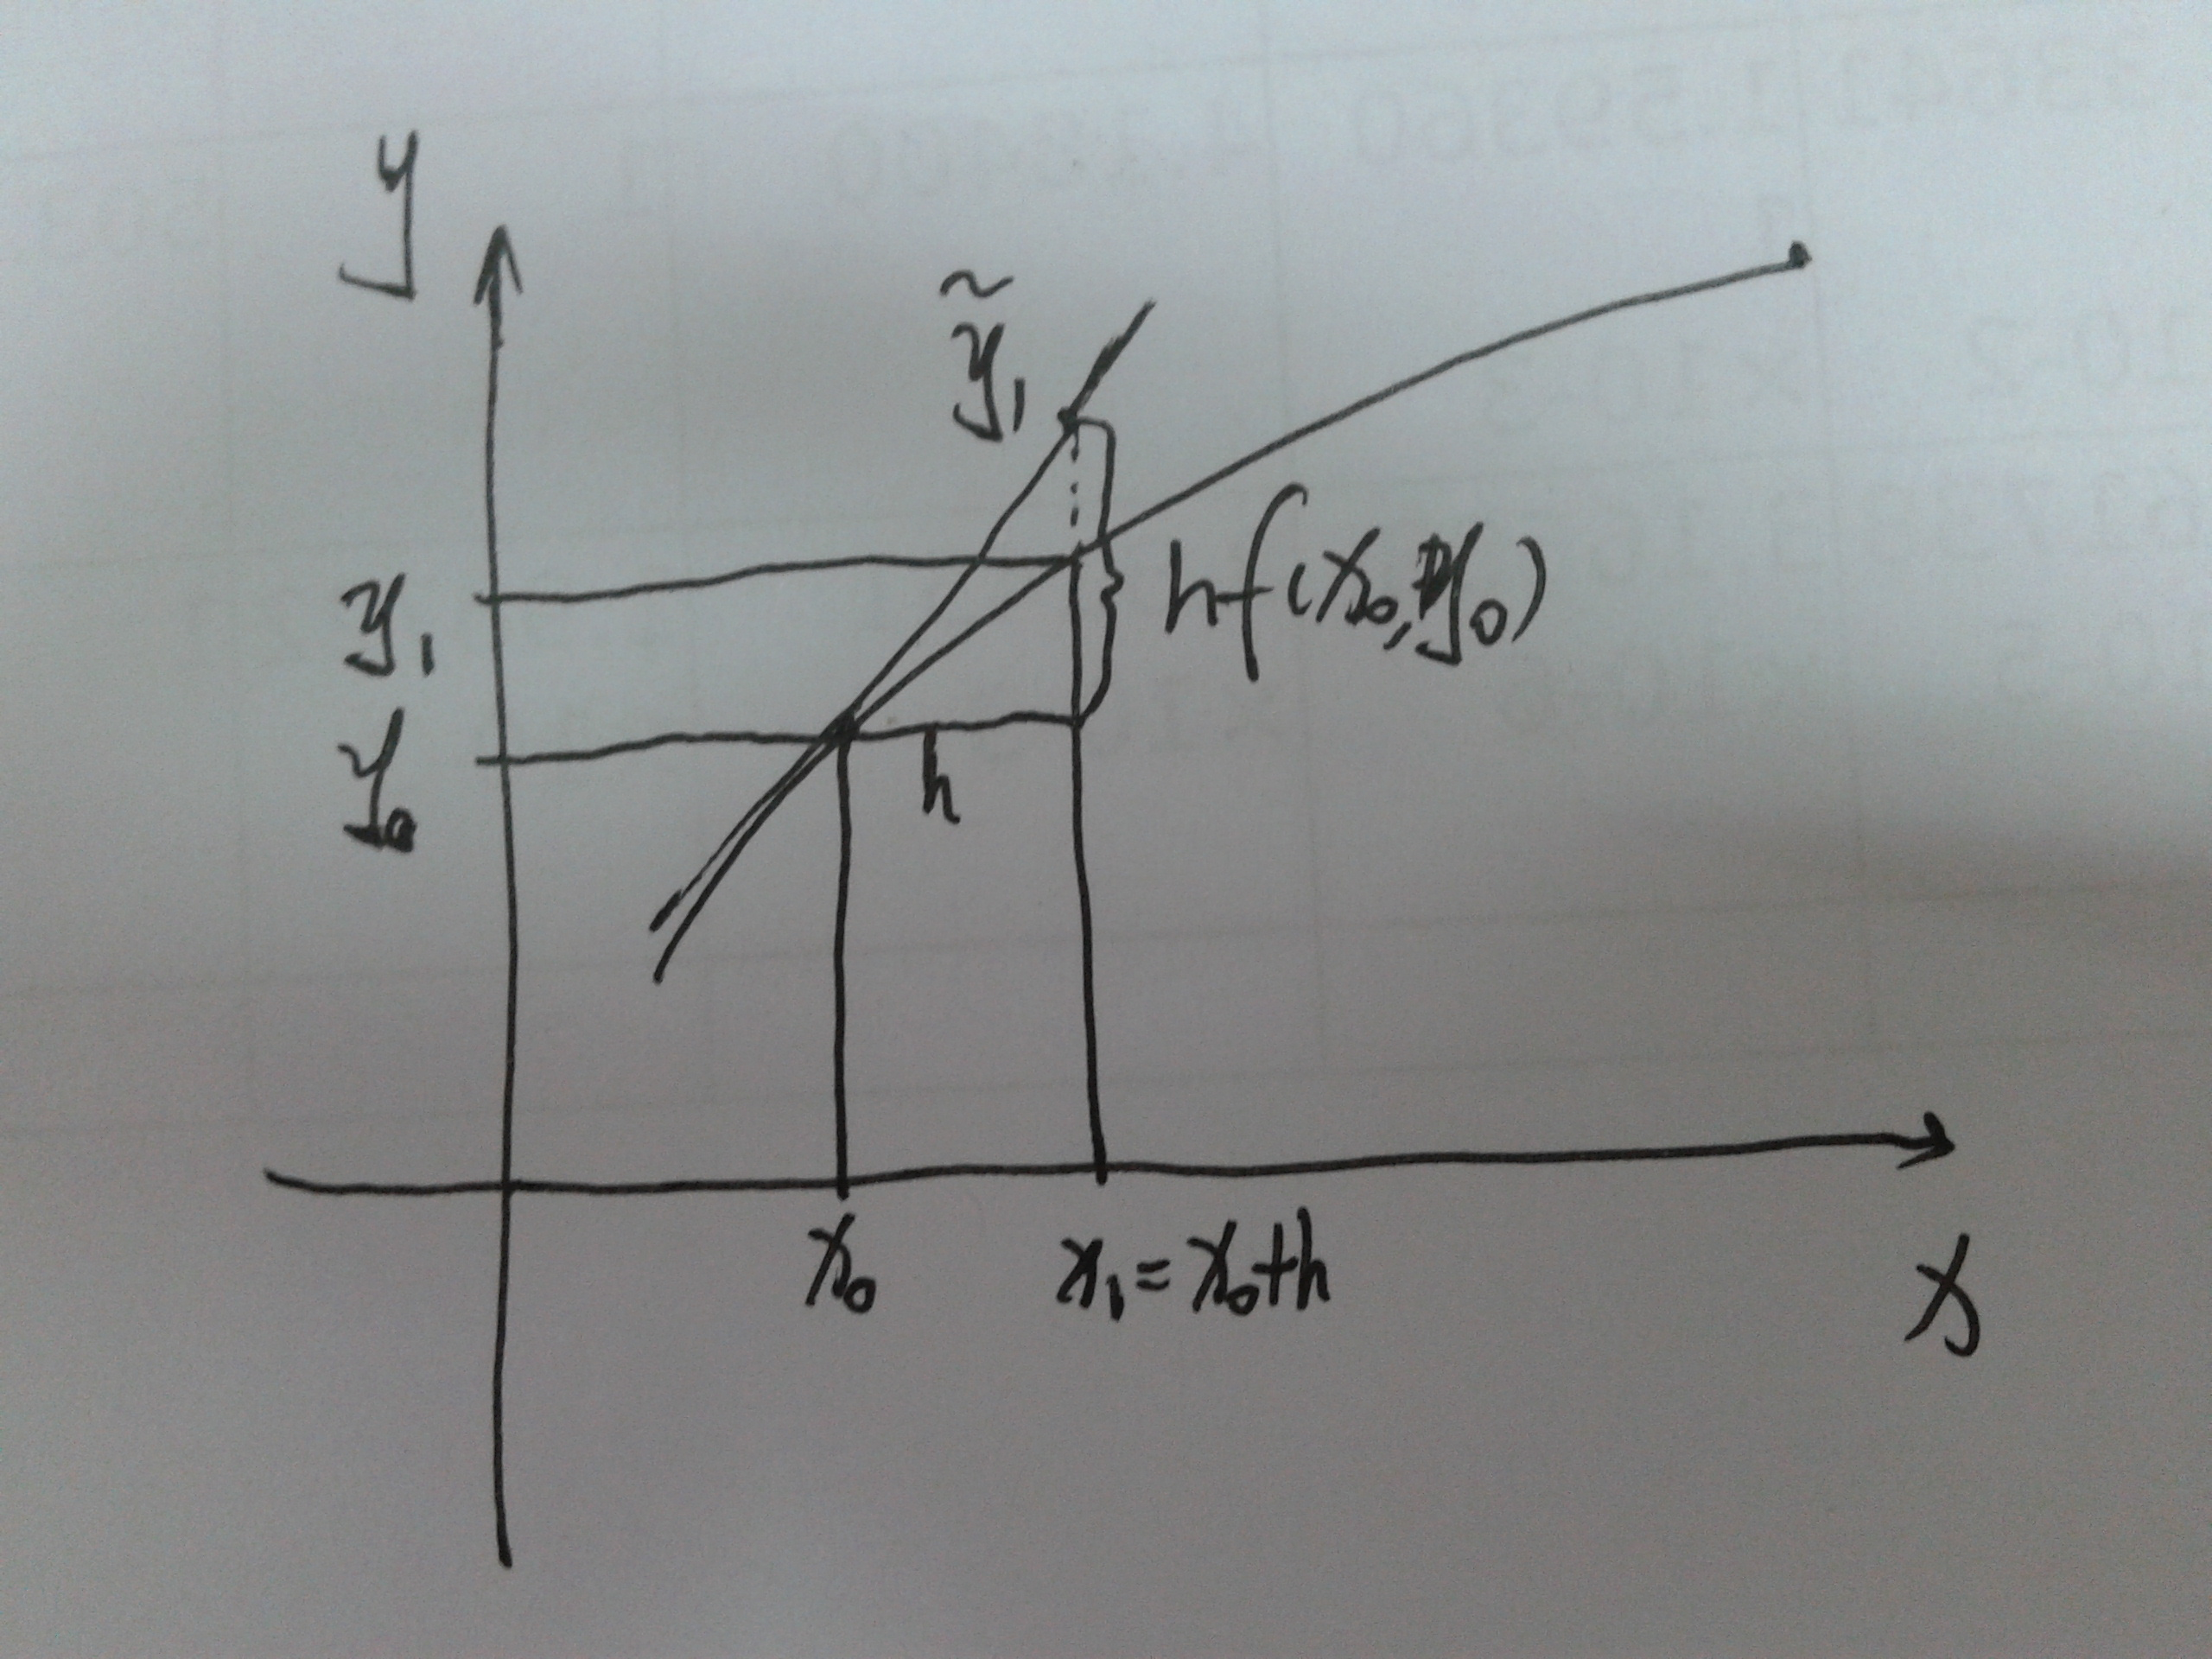
\includegraphics[width=0.7\textwidth]{pictures/2012-07-25.jpg}


有:
$$\tilde{y}_1=y_0+hf(x_0,y_0)\sim y_1$$
近似有:
$$y_{n+1}= y_n+h f(x_n,y_n)$$
这就是欧拉公式。

如果将步长$h$取的很小,与初始值相邻的第一个值$(x_1,y_1)$求得的近似值$(x_1,\tilde{y}_1)$可以说是非常精确的。但之后一的求解是将近似值$(x_1,\tilde{y}_1)$作为初始值进行计算,很明显,正在越来越偏离准确值,非常大的误差正在形成。这一点在后面的具体例子中可以明显看出。



\subsection{后退欧拉法(隐式)}
对$\frac{dy}{dx}=f(x,y)$从$x_n$到$x_{n+1}$积分,得
$$y(x_{n+1})=y(x_n)+\int_{x_n}^{x_{n+1}}f(t,y(t))dt$$
将右端的积分用右矩形公式$hF(x_{n+1},y(x_{n+1}))$代替,得
$$y_{n+1}=y_n+hf(x_{n+1},y_{n+1})$$
这个公式称为后退欧拉公式。

后退欧拉公式与欧拉公式有着本质的区别,欧拉公式是关于$y_{n+1}$的一个直接的计算公式,这类公式称作是\textbf{显式的}。后退欧拉公式右端含有未知的$y_{n+1}$,实际上是关于$y_{n+1}$的一个函数方程,这类公式称作是\textbf{隐式的}。

隐式方程通常用迭代法求解,而迭代过程的实质是逐步显式化。

\subsubsection{迭代法对后退欧拉公式求解}
\textbf{求解过程}

1、先用欧拉公式给出迭代初值$y_{n+1;0}$(前面已经说过,欧拉公式给出的第一个相邻值还是非常精确的)
$$y_{n+1;0}=y_n+hf(x_n,y_n)$$
其中下标中分号“;”后的数字表示迭代次数。

2、将迭代初值$y_{n+1;0}$代入后退欧拉公式
$$y_{n+1;1}=y_n+hf(x_{n+1},y_{n+1;0})$$


3、如此反复进行,得
$$y_{n+1;k+1}=y_n+hf(x_{n+1};y_{n+1;k}) \qquad (k=0,1,\cdots)$$

看到这个迭代过程,很容易产生一个问题:这样迭代求出的解是不是趋进于精确解,即是否收敛?下面就来讨论。



\textbf{解的收敛性}

由于$f(x,y)$对$y$满足利普希茨(Lipschitz)条件
$$|f(x,y)-f(x,\tilde{y})|\le L|y-\tilde{y}|$$
$L$是$f(x,y)$关于$y$的利普希茨常数。$L$的具体数值如何确定?

将$y_{n+1;k+1}=y_n+hf(x_{n+1};y_{n+1;k})$减去$y_{n+1}=y_n+hf(x_{n+1},y_{n+1})$即,将迭代$k$后的后退欧拉公式减去还未迭代的后退欧拉公式,有
$$|y_{n+1;k+1}-y_{n+1}|=h|f(x_{n+1},y_{n+1;k+1})-f(x_{n+1},y_{n+1})|
\le hL|y_{n+1,k}-y_{n+1}|$$
这个公式可以看出,只要$hL<1$,每次迭代出的解都比上一次迭代出的解趋近与精确解,即,后退欧拉法的迭代公式收敛到精确解。



\subsection{梯形公式(隐式)}
对$\frac{dy}{dx}=f(x,y)$从$x_n$到$x_{n+1}$积分,得
$$y(x_{n+1})=y(x_n)+\int_{x_n}^{x_{n+1}}f(t,y(t))dt$$
为了得到比后退欧拉法精度更高的计算公式,右端积分用梯形求积公式近似(梯形是比矩形更准确些)
$$y_{n+1}=y_n+\frac{h}{2}[f(x_n,y_n)+f(x_{n+1},y_{n+1})]$$
这个公式称为梯形公式。

梯形公式也是隐式的,也用迭代法求解,仍用欧拉公式提供迭代初值,其迭代公式为
$$\begin{cases}y_{n+1;0}=y_n+hf(x_n,y_n)\\
y_{n+1;k+1}=y_n+\frac{h}{2}[f(x_n,y_n)+f(x_{n+1},y_{n+1;k})]\\
(k=0,1,2\cdots)\end{cases}$$

梯形迭代公式解的收敛性讨论:

与后退欧拉公式迭代求解差不多,只不过这里是将未迭代的公式减去迭代$k$后的公式,
$$y_{n+1}-y_{n+1;k+1}=\frac{h}{2}[f(x_{n+1,y_{n+1}})-f(x_{n+1},y_{n+1;k})]$$
利用利普希茨条件$|f(x,y)-f(x,\tilde{y})|\le L|y-\tilde{y}|$,有
$$|y_{n+1}-y_{n+1;k+1}|\le \frac{hL}{2}|y_{n+1}-y_{n+1;k}|$$
由此可知,如果选取$h$充分小,使得$\frac{hL}{2}<1$,则当$k\rightarrow \infty$时,有$y_{n+1;k+1}\rightarrow y_{n+1}$,即梯形迭代公式是收敛的。



\subsection{改进欧拉法}
梯形方法虽然提高了精度,但其算法复杂,在应用梯形迭代公式进行实际计算时,没迭代一次,都要重新计算函数$f(x,y)$的值,而迭代又要反复进行若干次,计算量很大,而且往往难以预测。为了控制计算量,通常只迭代一两次就转入下一步的计算,这就简化了算法。

\textbf{思路如下:}

先用欧拉公式求得一个初步的近似值$\tilde{y}_{n+1}$,称之为\textbf{预测值}。预测值$\tilde{y}_{n+1}$的精度可能很差,在用梯形公式将它校正一次,即迭代一次得$y_{n+1}$,这个结果称为\textbf{校正值}。这样建立的预测-校正系统称为\textbf{改进的欧拉公式:}
\begin{align*}
&\text{预测}\qquad \tilde{y}_{n+1}=y_n+hf(x_n,y_n)=y_p\\
&\text{校正}\qquad y_{n+1}=y_n+\frac{h}{2}[f(x_n,y_n)+f(x_{n+1},\tilde{y}_{n+1})]
\end{align*}
即:
$$y_{n+1}=\frac{y_n}{2}+\frac{h}{2}f(x_n,y_n)+\frac{y_n}{2}+\frac{h}{2}f(x_{n+1};\tilde{y}_{n+1})$$
由此改写成平均化形式为
$$\begin{cases}
y_p = y_n+hf(x_n,y_n)\\
y_c = y_n+hf(x_{n+1},y_p)\\
y_{n+1}=\frac{1}{2}(y_p+y_c)
\end{cases}$$
其中$p$表示prediciton,$c$表示correction。




\subsection{单步法的局部截断误差与阶}
初值问题$\begin{cases}\cfrac{dy}{dx}=f(x,y),&a\le x\le b\\ y(a)=c &\end{cases}$单步法的一般形式为:
$$y_{n+1}=y_n+h\varphi(x_n,y_n,y_{n+1},h)$$
其中多元函数$\varphi$与$f(x,y)$有关。

当$\varphi$含有$y_{n+1}$时,方法是隐式的。若不含$y_{n+1}$则为显式方法,该\textbf{显式单步法}表示为:
$$y_{n+1}=y_n+h\varphi(x_n,y_n,h)$$
$\varphi(x,y,h)$称为增量函数,例如欧拉法有$\varphi(x,y,h)=f(x,y)$。

对一般显式单步法局部截断误差定义如下:

\textbf{定义1}

设$y(x)$是初值问题$\begin{cases}\cfrac{dy}{dx}=f(x,y),&a\le x\le b\\
y(a)=c &\end{cases}$的准确解,假设在$x_n$前各步没有误差,即$y_n$是准确解$y(x_n)$。$x_n$下一步的数值解为:$y_{n+1}=y_n+h\varphi(x_n,y_n,h)$,将精确解$y(x_{n+1})$减去数值解$y_{n+1}$就得到计算这步的误差:
$$T_{n+1}=y(x_{n+1})-y(x_n)-h\varphi(x_n,y(x_n),h)$$
$T_{n+1}$称为显式单步法$y_{n+1}=y_n+h\varphi(x_n,y_n,h)$的局部截断误差。从定义可以看出,$T_{n+1}$之所以称为局部截断误差是因为它反映的是显式单步法计算一步时的误差。

$T_{n+1}$的表达式是很好理解的,$y(x_{n+1})-y(x_n)$表示的是从$x_n$步到$x_{n+1}$精确解间的差值。而$h\varphi(x_n,y_n,h)$表示的是从$x_n$步到$x_{n+1}$数值解间的差值(前提假设是$x_n,y_n$是精确解,$x_n,y_n$可以理解为这步数值计算的初值)。由此这步精确解间的差值和这步数值解间的差值之差反映的当然是这步数值计算的误差,而反映的误差只限于这一步计算,故称为局部误差。

但是实际计算中$y_n$并不是精确解,这个误差定义也就是初值$x_0,y_0$的下一步$x_1,y_1$严格满足。……例子中算算步误差是否在这个误差定义的范围内……


\textbf{定义2}

设$y(x)$是初值问题$\begin{cases}\cfrac{dy}{dx}=f(x,y),&a\le x\le b\\y(a)=c &\end{cases}$的准确解,若存在最大整数$p$使显式单步法的局部截断误差满足
$$T_{n+1}=y(x+h)-y(x)-h\varphi(x,y,h)=O(h^{p+1})$$
则称显式单步法具有$p$阶精度。若将上式写成
$$T_{n+1}=\psi(x_n,y(x_n))h^{p+1}+O(h^{p+2})$$
则$\psi(x_n,y(x_n))h^{p+1}$称为局部截断误差主项。这样的形式对误差的表示是很有意义的,就$T_{n+1}$而言,其本身就是个小量,这个小量中,又存在更高阶的小量$O(h^{p+2})$,故实际讨论中,可以将这个更高阶小量$O(h^{p+2})$略去,余下的局部截断误差主项$\psi(x_n,y(x_n))h^{p+1}$已经就能很好的描述误差了。

\subsubsection{欧拉法的局部截断误差}
欧拉公式为:
$$y_{n+1}=y_n+hf(x_n,y_n)$$

利用定义1,有:
$$T_{n+1}=y(x_{n+1})-y(x_n)-hf(x_n,y(x_n))$$
将$y(x_{n+1})=y(x_n+h)$在$x_n$用泰勒展开:
\begin{align*}
y(x_{n+1})=y(x_n+h)&=y(x_n)+y\rq{}(x_n)(x_n+h-x_n)+\frac{y\rq{}\rq{}(x_n)}{2!}(x_n+h-x_n)^2+O(h^3)\\
&=y(x_n)+hy\rq{}(x_n)+\frac{h^2}{2}y\rq{}\rq{}(x_n)+O(h^3)
\end{align*}
将$f(x_n,y(x_n))$改写$y\rq{}(x_n)$\footnote{$f(x_n,y(x_n))$=$y\rq{}(x_n)$,$f(x,y)$就是$y(x)$的斜率,看原方程就知道了。},于是,有:
$$T_{n+1}=\frac{h^2}{2}y\rq{}\rq{}(x_n)+O(h^3)$$
根据定义2,局部截断误差主项为$\cfrac{\hbar^2}{2}y\rq{}\rq{}(x_n)$。就整个$T_{n+1}$而言,将高阶项$O(h^3)$略去($T_{n+1}$本来就是小量),则$T_{n+1}=O(h^2)$。根据定义$p=1$,即欧拉法是1阶方法。



\subsubsection{后退欧拉法局部截断误差}
后退欧拉公式为:
$$y_{n+1}=y_n+hf(x_{n+1},y_{n+1})$$

利用定义1,有:
$$T_{n+1}=y(x_{n+1})-y(x_n)-hf(x_{n+1},y(x_{n+1}))$$
将$y(x_{n+1})=y(x_n+h),f(x_{n+1},y(x_{n+1}))=y\rq{}(x_{n+1})=y\rq{}(x_n+h)$在$x_n$处泰勒展开,有:
\begin{align*}
y(x_{n+1})=y(x_n+h)&=y(x_n)+y\rq{}(x_n)(x_n+h-x_n)+\frac{y\rq{}\rq{}(x_n)}{2!}(x_n+h-x_n)^2+O(h^3)\\
&=y(x_n)+hy\rq{}(x_n)+\frac{h^2}{2}y\rq{}\rq{}(x_n)+O(h^3)
\end{align*}
\begin{align*}
f(x_{n+1},y(x_{n+1}))&=y\rq{}(x_{n+1})=y\rq{}(x_n+h)
=y\rq{}(x_n)+hy\rq{}\rq{}(x_n)+O(h^2)
\end{align*}
代入$T_{n+1}$中,有:
\begin{align*}
T_{n+1}&=y(x_n)+hy\rq{}(x_n)+\frac{h^2}{2}y\rq{}\rq{}(x_n)+O(h^3)
-y(x_n)-h[y\rq{}(x_n)+hy\rq{}\rq{}(x_n)+O(h^2)]\\
&=-\frac{h^2}{2}y\rq{}\rq{}(x_n)+O(h^3)
\end{align*}
这里$O(h^2)$直接抹去了,是因为有更高阶的小量$O(h^3)$在。

按照定义2,$p=1$,是1阶方法,局部截断误差主项为$-\cfrac{h^2}{2}y\rq{}\rq{}(x_n)$。



\subsubsection{梯形法局部截断误差}
梯形公式为:
$$y_{n+1}=y_n+\frac{h}{2}[f(x_n,y_n)+f(x_{n+1},y_{n+1})]$$
利用定义1,有:
$$T_{n+1}=y(x_{n+1})-y(x_n)-\frac{h}{2}[y\rq{}(x_n)+y\rq{}(x_{n+1})]$$
将$y(x_{n+1})=y(x_n+h),f(x_{n+1},y(x_{n+1}))=y\rq{}(x_{n+1})=y\rq{}(x_n+h)$在$x_n$处泰勒展开,有:
\begin{align*}
&y(x_n+h)=y(x_n)+hy\rq{}+h^2\frac{y\rq{}\rq{}(x_n)}{2!}+h^3\frac{y\rq{}\rq{}\rq{}(x_n)}{3!}+O(h^4)\\
&f(x_{n+1},y(x_{n+1}))=y\rq{}(x_{n+1})=y\rq{}(x_n+h)
=y\rq{}(x_n)+hy\rq{}\rq{}(x_n)+\frac{h^2}{2}y\rq{}\rq{}\rq{}(x_n)+O(h^3)
\end{align*}
这里为什么展开的级数和上面两个不一样,那是因为必须凑成定义2的形式,从上式看的到$y\rq{}(x_n),y\rq{}\rq{}(x_n)$都相消为0了。

代入$T_{n+1}$中,有:
\begin{align*}
T_{n+1}=&y(x_n)+hy\rq{}+h^2\frac{y\rq{}\rq{}(x_n)}{2!}+h^3\frac{y\rq{}\rq{}\rq{}(x_n)}{3!}+O(h^4)-y(x_n)\\
& -\frac{h}{2}[y\rq{}(x_n)+y\rq{}(x_n)+hy\rq{}\rq{}(x_n)+\frac{h^2}{2}y\rq{}\rq{}\rq{}(x_n)+O(h^3)]\\
=&\frac{h^3}{6}y\rq{}\rq{}\rq{}(x_n)-\frac{h^3}{4}y\rq{}\rq{}\rq{}(x_n)+O(h^3)\\
=&-\frac {h^3}{12}y\rq{}\rq{}\rq{}(x_n)+O(h^4)
\end{align*}
根据定义2,梯形法是二阶的,其局部误差主项为$-\cfrac {h^3}{12}y\rq{}\rq{}\rq{}(x_n)$。



\section{龙格—库塔法}
\subsection{显式龙格-库塔法的一般形式}
方程
$$\begin{cases}\cfrac{dy}{dx}=f(x,y),&a\le x\le b\\ y(a)=c &\end{cases}$$
等价积分形式为
$$y(x_{n+1})=y(x_n)+\int_{x_n}^{x_{n+1}}f(x,y(x))dx$$
若要是公式阶数提高,就必须使右端积分的数值求积公式精度提高,它必然要增加求积节点,为此将上式右端用求积公式表示为
$$\int_{x_n}^{x_{n+1}}f(x,y(x))dx\approx h\sum_{i=1}^r c_i f(x_n+\lambda_i h,y(x_n+\lambda_i h))$$
\textbf{这个公式应该是龙格库塔法思想的核心。}这个公式给人感觉是在由$x_n$到$x_{n+1}$步中又分出个$r$步计算,增加步数当然能提高精度了。

为了得到便于计算的显式方法,类似改进欧拉法
$$y_{n+1}=y_n+\frac{h}{2}[f(x_n,y_n)+f(x_n+h,y_n+hf(x_n,y_n))]$$

将$y_{n+1}$表示为
$$y_{n+1}=y_n+h\varphi(x_n,y_n,h)$$
其中
$$\varphi(x_n,y_n,h)=\sum_{i=1}^rc_iK_i,
\qquad K_1=f(x_n,y_n),
\qquad K_i=f(x_n+\lambda_i h, y_n+h\sum_{j=1}^{i-1}\mu_{ij}K_j)
\qquad i=2,\cdots,r$$
这里$c_i,\lambda_i,\mu_{ij}$均为常数。这个公式称为$r$级显式龙格-库塔法(Runge-Kutta),简称R-K法。

当$r=1$,$\varphi(x_n,y_n,h)=f(x_n,y_n)$,是欧拉法,此时方法的阶为$p=1$。



\subsection{二阶显式R-K法}
当$r=2$时,由$r$级显式龙格-库塔法,有
$$\begin{cases}y_{n+1}=y_n+h(c_1K_1+c_2K_2) \\
K_1=f(x_n,y_n)\\
K_2=f(x_n+\lambda_2h,y_n+\mu_{21}hK_1)
\end{cases}$$
这里$c_1,c_2,\lambda_2,\mu_{21}$均为待定常数,不同系数有不同表达式。可见改进欧拉法就是一种二阶显式龙格-库塔法。适当选取这些系数,是公式阶数$p$尽量高,通过局部截断误差来确定这些系数。

根据局部截断误差的定义,其局部截断误差为
$$T_{n+1}=y(x_{n+1})-y(x_n)-h[c_1f(x_n,y_n)+c_2f(x_n+\lambda_2h,y_n+\mu_{21}hf_n)]$$
其中$y_n=y(x_n),f_n=f(x_n,y_n)$。

为得到$T_{n+1}$的阶$p$,将上式各项在$(x_n,y_n)$处做泰勒展开\footnote{为什么不像后退欧拉法和梯形法,化成$y(x_n+h)$的形式,在$x_n$处泰勒展开?那是因为寻找处阶$p$的目标是化成局部截断误差定义2的形式,这里的项$f(x_n+\lambda_2h,y_n+\mu_{21}hf_n)$是没办法搞成这种形式。后退欧拉法和梯形法只需$y(x_n)$各级导数形式就达成这个目标了,不需要用$f(x_n,y_n)$二元泰勒展开,展开也是多此一举,会相消掉。},由于$f(x,y)$是二元函数,用二元泰勒展开,各项展开式为
\begin{align*}
y(x_{n+1}) = y(x_n+h)=y_n+hy\rq{}+\frac{h^2}{2}y\rq{}\rq{}_n+\frac{h^3}{3!}y\rq{}\rq{}\rq{}_n+O(h^4)
\end{align*}
其中
$$\begin{cases}
y\rq{}_n =f(x_n,y_n)=f_n\\
y\rq{}\rq{}_n=\frac{\partial}{\partial x}y\rq{}_n=\frac{\partial}{\partial x}f(x_n,y_n)=f\rq{}_x(x_n,y_n)+f\rq{}_y(x_n,y_n)\cdot y\rq{}_n=f\rq{}_x(x_n,y_n)+f\rq{}_y(x_n,y_n)\cdot f_n\\
y\rq{}\rq{}\rq{}_n=f\rq{}\rq{}_{xx}(x_n,y_n)+f\rq{}\rq{}_{xy}(x_n,y_n)y\rq{}_n
+f\rq{}\rq{}_{yx}(x_n,y_n)f_n+f^2_nf\rq{}\rq{}_{yy}(x_n,y_n)\\
\qquad\qquad+f\rq{}_y(x_n,y_n)[f\rq{}_x(x_n,y_n)+f\rq{}_y(x_n,y_n)\cdot f(x_n,y_n)]\\
\qquad =f\rq{}\rq{}_{xx}(x_n,y_n)+2f_nf\rq{}_{xy}(x_n,y_n)+f^2_nf\rq{}\rq{}_{yy}(x_n,y_n)+f\rq{}_y(x_n,y_n)[f\rq{}_x(x_n,y_n)+f_nf\rq{}_y(x_n,y_n)]
\end{cases}$$
注意推导时多次用到第一个式子$y\rq{}_n =f(x_n,y_n)=f_n$替换,还有$f\rq{}\rq{}_{xy}(x_n,y_n)$和$f\rq{}\rq{}_{yx}(x_n,y_n)$是相等的,求导顺序不影响结果。
\begin{align*}
f(x_n+\lambda_2h,y_n+\mu_21hf_n)
=f_n+f\rq{}_x(x_n,y_n)\lambda_2h+f\rq{}_y(x_n,y_n)\mu_{21}hf_n+O(h^2)
\end{align*}

观察$f(x_n+\lambda_2h,y_n+\mu_{21}hf_n)$发现$y(x_{n+1})$展开到4阶时,$y\rq{}\rq{}\rq{}_n$项中的$f\rq{}_yf\rq{}_x+f\rq{}_yf$不能通过选择参数消掉,也就说$r=2$的龙格-库塔公式不能使局部误差提高到$O(h^4)$。实际上要使$h^3$项为零,需增加3个方程,要确定4个参数$c1,c_1,\lambda_2$及$\mu_{21}$,这是不可能的。故$r=2$的显式龙格-库塔法的阶只能是$p=2$,而不能得到三阶公式。

$y(x_{n+1})$最多只能展开到2阶,即:
\begin{align*}
y(x_{n+1}) = y(x_n+h)=y_n+hy\rq{}+\frac{h^2}{2}y\rq{}\rq{}_n+O(h^3)
\end{align*}
代入到$T_{n+1}$,有
\begin{align*}
T_{n+1}=&y_n+hy\rq{}+\frac{h^2}{2}y\rq{}\rq{}_n+O(h^3)-y(x_n)\\
&-h\{c_1f(x_n,y_n)
+c_2[f_n+f\rq{}_x(x_n,y_n)\lambda_2h+f\rq{}_y(x_n,y_n)\mu_{21}hf_n+O(h^2)]\}\\
=&y_n+hf_n+\frac{h^2}{2}[f\rq{}_x(x_n,y_n)+f\rq{}_y(x_n,y_n)\cdot f_n]+O(h^3)-y(x_n)\\
&-h\{c_1f(x_n,y_n)
+c_2[f_n+f\rq{}_x(x_n,y_n)\lambda_2h+f\rq{}_y(x_n,y_n)\mu_{21}hf_n+O(h^2)]\}\\
=&(1-c_1-c_2)f_nh+\left(\frac{1}{2}-c_2\lambda_2\right)f\rq{}_x(x_n,y_n)h^2-\left(\frac{1}{2}-c_2\mu_{21}\right)f\rq{}_y(x_n,y_n)f_nh^2+O(h^3)
\end{align*}
要使$p=2$阶,必须使
$$1-c_1-c_2=0,\qquad \frac{1}{2}-c_2\lambda_2=0,\qquad \frac{1}{2}-c_2\mu_{21}=0$$
即
$$c_2\lambda_2=\frac{1}{2} ,\qquad c_2\mu_{21}=\frac{1}{2} ,\qquad c_1+c_2=1$$
它的解不是唯一的,令$c_2=a\ne 0$,则
$$c_1=1-a ,\qquad \lambda_2=\mu_{21}=\frac{1}{2a} $$
这样得到的公式称为二阶龙格-库塔法。

如果取$a=\frac{1}{2}$,则$c_1=c_2=\frac{1}{2} ,\lambda_2=\mu_{21}=1$,这就是改进欧拉法。

若取$a=1$,则$c_2=1,c_1=0,\lambda_2=\mu_{21}=\frac{1}{2}$,得到计算公式
$$\begin{cases}
y_{n+1}=y_n+hK_2\\
K_1=f(x_n,y_n)\\
K_2=f(x_n+\frac{h}{2},y_n+\frac{h}{2}K_1)
\end{cases}$$
称为中点公式,相当与数值积分的中矩形公式,也可以表示为
$$y_{n+1}=y_n+hf(x_n+\frac{h}{2},y_n+\frac{h}{2}f(x_n,y_n)$$



\subsection{三阶显式龙格-库塔法}
$r=3$可以得到三阶显式龙格-库塔法,其表达式为
$$\begin{cases}
y_{n+1}=y_n+h(c_1K_1+c_2K_2+c_3K_3)\\
K_1=f(x_n,y_n)\\
K_2=f(x_n+\lambda_2h,y_n+\mu_{21}hK_1)\\
K_3=f(x_n+\lambda_3h,y_n+\mu_{31}hK_1+\mu_{32}hK_2)
\end{cases}$$
其中$c_1,c_2,c_3$及$\lambda_2,\mu_{21},\lambda_3,\mu_{31},\mu_{32}$均为待定参数。该公式的局部截断误差为
$$T_{n+1}=y(x_{n+1})-y(x_n)-h[c_1K_1+c_2K_2+c_3K_3]$$
将$K_2,K_3$按二元函数泰勒展开,使$T_{n+1}=O(h^4)$,可得待定参数满足方程
$$\begin{cases}
c_1+c_2+c_3=1\\
\lambda_2=\mu_{21}\\
\lambda_3=\mu_{31}+\mu_{32}\\
c_2\lambda_2+c_3\lambda_3=\frac{1}{2}\\
c_2\lambda_2^2+c_3\lambda_3^2=\frac{1}{3}\\
c_3\lambda_2\mu_{32}=\frac{1}{6}
\end{cases}$$
这是8个未知数6个方程的方程组,解也不是唯一的,可以得到很多公式,这些公式统称为三阶龙格-库塔公式。

常见的三阶龙格-库塔公式为
$$\begin{cases}
y_{n+1}=y_n+\frac{h}{6}(K_1+4K_2+K_3)\\
K_1=f(x_n,y_n)\\
K_2=f(x_n+\frac{h}{2},y_n+\frac{h}{2}K_1)\\
K_3=f(x_n+h,y_n-hK_1+2hK_2)
\end{cases}$$



\subsection{四阶龙格-库塔法}
类似二阶、三阶龙格-库塔法推导过程可以推导出各种四阶龙格-库塔公式,常用公式为
$$\begin{cases}
y_{n+1}=y_n+\cfrac{h}{6}(K_1+2K_2+2K_3+K_4)\\
K_1=f(x_n,y_n)\\
K_2=f(x_n+\cfrac{h}{2},y_n+\cfrac{h}{2}K_1)\\
K_3=f(x_n+\cfrac{h}{2},y_n+\cfrac{h}{2}K_2)\\
K_4=f(x_n+h,y_n+hK_3)
\end{cases}
$$
其截断误差为$O(h^5)$。二阶的推导已经比较烦了,四阶推导可以想象有多烦。有的地方采用如下表达式
$$\begin{cases}y_1=y_0+\frac{1}{6}(K_0+2\times K_1 +2\times K_2 + K_3)\\
K_0=h \times f(x_0,y_0)\\
K_1=h \times f(x_0+\frac{h}{2},y_0+\frac{K_0}{2})\\
K_2=h \times f(x_0+\frac{h}{2},y_0+\frac{K_1}{2})\\
K_3=h \times f(x_0+h,y_0+K_2)
\end{cases}$$



\section{各种方法的应用举例及对比}
求解初值问题
$$\begin{cases}y\rq{}=y-\frac{2x}{y} &(0\le x \le 1)\\ y(0)=1\end{cases}$$



\subsection{精确解}
初值问题
$$\begin{cases}y\rq{}=y-\frac{2x}{y} &(0\le x \le 1)\\ y(0)=1\end{cases}$$
精确解为
$$y=\sqrt{1+2x} \qquad 0\le x \le 1$$
取步长为0.1其结果为
\begin{figure}[htb]
\begin{minipage}[b]{0.5\textwidth}
\centering
\begin{tabular}{c|c}
$x_n$ & $y(x_n)$\\
\hline
 0.0     &      1.000000\\
 0.1	&	1.095445\\
0.2	&	1.183216\\
0.3	&	1.264911\\
0.4	&	1.341641\\
0.5	&	1.414214\\
0.6	&	1.483240\\
0.7	&	1.549193\\
0.8	&	1.612452\\
0.9	&	1.673320\\
1.0	&	1.732051\\
\end{tabular}
\caption{精确解}
\end{minipage}%
\begin{minipage}[b]{0.5\textwidth}
\centering
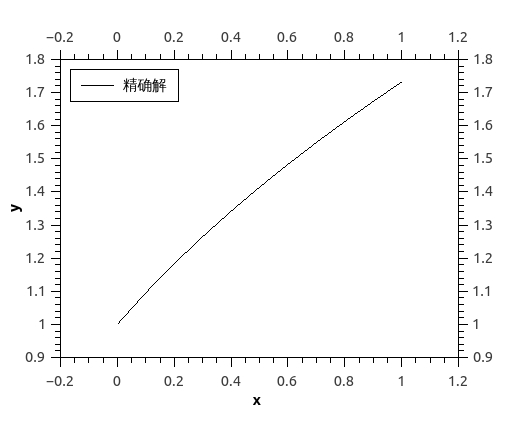
\includegraphics[width=0.9\textwidth]{program/numerical_analysis_examples/exact_solution.jpeg}
\caption{精确解}
\label{fig:by:table}
\end{minipage}
\end{figure}

Fortran代码如下:
\lstinputlisting{program/numerical_analysis_examples/exact_solution.f90}



\subsection{欧拉法求解}
对于解初值问题
$$\begin{cases}y\rq{}=y-\frac{2x}{y} &(0 \le x \le 1)\\ y(0)=1\end{cases}$$
的欧拉公式的具体形式为
$$y_{n+1}=y_n+h(y_n-\frac{2x_n}{y_n})$$
取步长为$h=0.1$其结果为

\begin{figure}[htb]
\begin{minipage}[b]{0.5\textwidth}
\centering
\begin{tabular}{c|c|c}
$x_n$ &       精确解($y_n$)   & 欧拉法解($y$)  \\
\hline
 0.0  &      1.000000       &	1.000000\\
 0.1	&	1.095445 	&	1.100000\\
0.2	&	1.183216 	&	1.191818\\
0.3	&	1.264911 	&	1.277438\\
0.4	&	1.341641	&	1.358213\\
0.5	&	1.414214	&	1.435133\\
0.6	&	1.483240	&	1.508966\\
0.7	&	1.549193	&	1.580338\\
0.8	&	1.612452	&	1.649784\\
0.9	&	1.673320	&	1.717780\\
1.0	&	1.732051	&	1.784771\\
\end{tabular}
\caption{精确解与欧拉法解}
\end{minipage}%
\begin{minipage}[b]{0.5\textwidth}
\centering
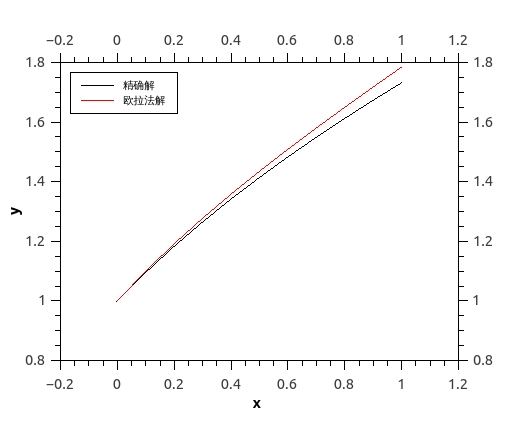
\includegraphics[width=0.9\textwidth]{program/numerical_analysis_examples/euler_method.jpeg}
\caption{精确解与欧拉法解}
\label{fig:by:table}
\end{minipage}
\end{figure}

Fortran代码如下:
\lstinputlisting[language=Fortran]{program/numerical_analysis_examples/euler_method.f90}



\subsection{改进欧拉法求解}
对于解初值问题
$$\begin{cases}y\rq{}=y-\frac{2x}{y} &(0 \le x \le 1)\\ y(0)=1\end{cases}$$
的改进欧拉公式的具体形式为
$$\begin{cases}
y_p=y_n+h(y_n-\frac{2x_n}{y_n})\\
y_c=y_n+h(y_p-\frac{2x_{n+1}}{y_p})\\
y_{n+1}=\frac{1}{2}(y_p+y_c)
\end{cases}$$
取步长$h=0.1$结果为

\begin{figure}[htb]
\centering
\begin{tabular}{c|c|c|c}
$x_n$ &       精确解($y_n$)   & 欧拉法解($y$)  & 改进欧拉法解($y$)\\
\hline
 0.0  &      1.000000       &	1.000000	&1.000000\\
 0.1	&	1.095445 	&	1.100000	&1.095909\\
0.2	&	1.183216 	&	1.191818	&1.184096\\
0.3	&	1.264911 	&	1.277438	&1.266201\\
0.4	&	1.341641	&	1.358213	&1.343360\\
0.5	&	1.414214	&	1.435133	&1.416402\\
0.6	&	1.483240	&	1.508966	&1.485955\\
0.7	&	1.549193	&	1.580338	&1.552514\\
0.8	&	1.612452	&	1.649784	&1.616474\\
0.9	&	1.673320	&	1.717780	&1.678166\\
1.0	&	1.732051	&	1.784771	&1.737867
\end{tabular}
\caption{精确解、欧拉法解、改进欧拉法解}
\centering
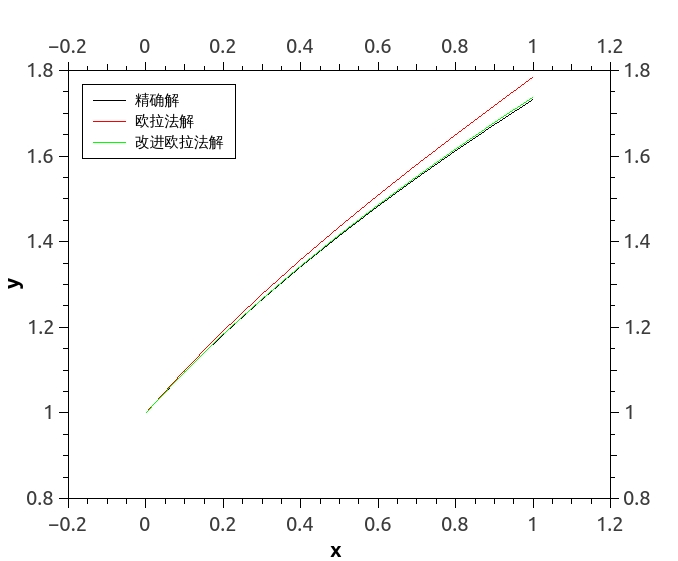
\includegraphics[width=0.7\textwidth]{program/numerical_analysis_examples/improved_euler_method.jpeg}
\caption{精确解、欧拉法解、改进欧拉法解}
\label{fig:by:table}
\end{figure}

Fortran代码如下:
\lstinputlisting[language=Fortran]{program/numerical_analysis_examples/improved_euler_method.f90}



\subsection{四阶龙格-库塔法求解}
对于解初值问题
$$\begin{cases}y\rq{}=y-\frac{2x}{y} &(0 \le x \le 1)\\ y(0)=1\end{cases}$$
的四阶龙格-库塔公式的具体形式为
$$\begin{cases}
y_{n+1}=y_n+\cfrac{h}{6}(K_1+2K_2+2K_3+K_4)\\
K_1=y_n-\cfrac{2x_n}{y_n}\\
K_2=y_n+\cfrac{h}{2}K_1-\cfrac{2x_n+h}{y_n+\cfrac{h}{2}K_1}\\
K_3=y_n+\cfrac{h}{2}K_2-\cfrac{2x_n+h}{y_n+\cfrac{h}{2}K_2}\\
K_4=y_n+hK_3-\cfrac{2(x_n+h)}{y_n+hK_3}
\end{cases}$$

Fortran代码如下:
\lstinputlisting[language=fortran]{program/numerical_analysis_examples/runge_kutta.f90}

取步长$h=0.1$结果为

\begin{figure}[htb]
\centering
\begin{tabular}{c|c|c|c|c}
$x_n$ &       精确解($y_n$)   & 欧拉法解($y$)  & 改进欧拉法解($y$) & 四阶龙格库塔法解($y$)\\
\hline
 0.0  &      1.000000       &	1.000000	&1.000000	&1.000000\\
 0.1	&	1.095445 	&	1.100000	&1.095909	&1.095446\\
0.2	&	1.183216 	&	1.191818	&1.184096	&1.183217\\
0.3	&	1.264911 	&	1.277438	&1.266201	&1.264912\\
0.4	&	1.341641	&	1.358213	&1.343360	&1.341642\\
0.5	&	1.414214	&	1.435133	&1.416402	&1.414215\\
0.6	&	1.483240	&	1.508966	&1.485955	&1.483242\\
0.7	&	1.549193	&	1.580338	&1.552514	&1.549196\\
0.8	&	1.612452	&	1.649784	&1.616474	&1.612455\\
0.9	&	1.673320	&	1.717780	&1.678166	&1.673324\\
1.0	&	1.732051	&	1.784771	&1.737867	&1.732056
\end{tabular}
\caption{精确解、欧拉法解、改进欧拉法解、四阶龙格库塔法解}
\centering
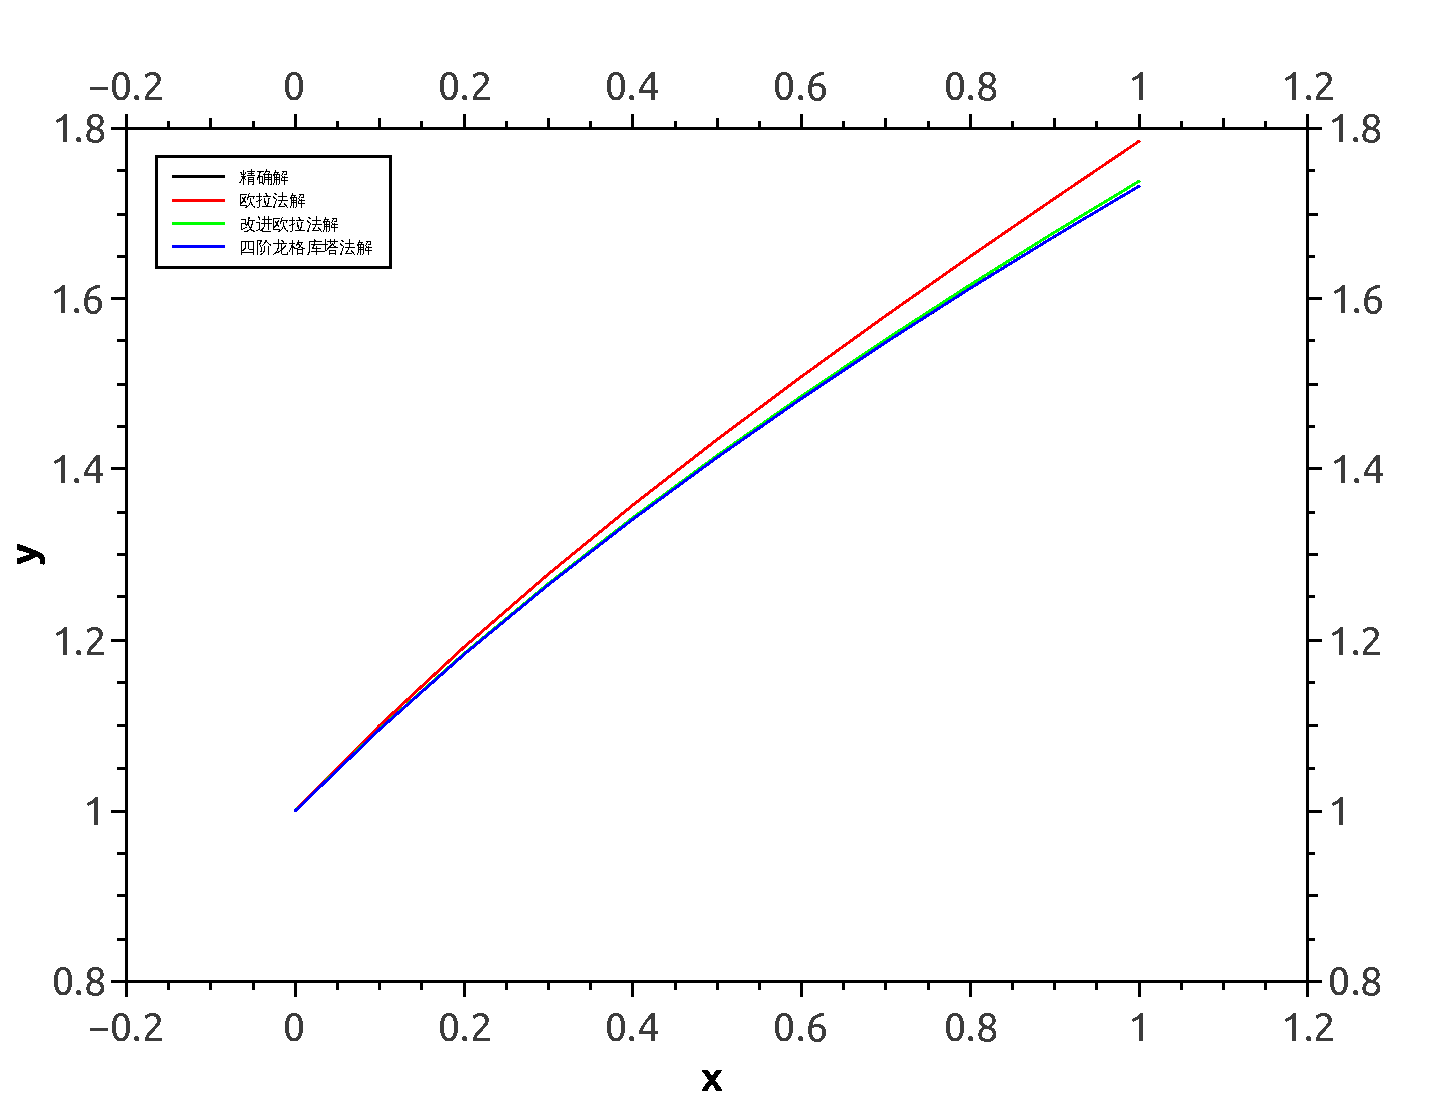
\includegraphics[width=1.0\textwidth]{program/numerical_analysis_examples/runge_kutta.pdf}
\caption{精确解、欧拉法解、改进欧拉法解、四阶龙格库塔法解}
\label{fig:by:table}
\end{figure}

四阶龙格库塔法的局部截断误差是$O(h^5)$,步长为$h=0.1$时,$h^5=0.00001$。

这个四阶龙格库塔的程序只适用于解这个问题,不具有普遍性,在四阶龙格库塔法程序章节中,将给出具有普遍性的四阶龙格库塔法的程序,而且适用于微分方程组。



\section{四阶龙格库塔法程序}

参考资料:《数值分析》(第4版),李庆扬,王能超,易大义 编;清华大学出版社


龙格-库塔法的推导基于泰勒展开,因而它要求所求的解具有较好的光滑性质。反之,如果解的光滑性差,那么实用四阶龙格-库塔法求得的数值解,其精度可以能反而不如改进的欧拉法。

一阶常微分方程的一般形式为:
$$\begin{cases}\cfrac{dy}{dx}=f(x,y),&a\le x\le b\\
y(a)=c &\end{cases}$$
在求解常微分方程时,通常会给出初始条件$x_0$及$y_0$。采用龙格库塔法求解常微分方程时,如果$x_1=x_0+h$,则对应的$y_1$为:
$$y_1=y_0+\frac{h}{6}(K_1+2\times K_2 +2\times K_3 + K_4)$$
其中4个参数为:
\begin{align*}
K_1&=f(x_0,y_0)\\
K_2&=f(x_0+\frac{h}{2},y_0+\frac{h}{2}K1)\\
K_3&=f(x_0+\frac{h}{2},y_0+\frac{h}{2}K2)\\
K_4&=f(x_0+h,y_0+hK_3)
\end{align*}

方程确定了,它的解也确定了\footnote{当然了,这个方程是有解的;还有就是有了初始条件或边界条件是唯一解,没这个是通解}。数值解是近似解,不同的步长有不同的精度,但是不管取何种步长,得出的解都是向精确解靠拢的。所以,当我们对同一个$x$值,用不同步长的到的$y$值相差很少时,说明这是时的解与精确解也相差很小,如果满足我们的精度需求,我们就可以取这时的$y$值。



\subsection{四阶龙格库塔法求解一阶微分方程组}

前面都是单个方程$y\rq{}=f$的数值解法,只要把$y$和$f$理解为向量,那么,所提供的各种计算公式即可应用到一阶方程组的情形。(还真没理解到?)

考察一阶方程组
$$y\rq{}_i=f_i(x,y_1,y_2,\cdots,y_N)\qquad (i=1,2,\cdots,N)$$
的初值问题,初始条件给为
$$y_i(x_0)=y_{i;0}\qquad (i=1,2,\cdots,N)$$
若采用向量的记号,记
$$\vec{y}=\begin{pmatrix}y_1 \\ y_2 \\ \vdots \\ y_N\end{pmatrix}
\qquad
\vec{y_0}=\begin{pmatrix} y_{1;0} \\ y_{2;0} \\  \vdots \\ y_{N;0} \end{pmatrix}
\qquad
\vec{f} =\begin{pmatrix} f_1 \\ f_2 \\ \vdots \\  f_N \end{pmatrix}$$
则上述方程组的初值问题可表示为
$$\begin{cases}\vec{y}\rq{}=\vec{f}(x,\vec{y}) \\ \vec{y}(x_0)=\vec{y}_0 \end{cases}$$
求解这一初值问题的四阶龙格-库塔公式为

(1)
$$\vec{y}_{n+1}=\vec{y}_n+\frac{h}{6}(\vec{k}_1+2\vec{k}_2+2\vec{k}_3+\vec{k}_4)$$
其中
$$\begin{cases}
\vec{k}_1 = \vec{f}(x_n,\vec{y}_n)\\
\vec{k}_2 = \vec{f}(x_n+\frac{h}{2},\vec{y}_n+\frac{h}{2}\vec{k}_1)\\
\vec{k}_3 = \vec{f}(x_n+\frac{h}{2},\vec{y}_n+\frac{h}{2}\vec{k}_2)\\
\vec{k}_4=\vec{f}(x_n+h,\vec{y}_n+h\vec{k}_3) 
 \end{cases}$$
或表示为

(2)
$$y_{i;n+1}=y_{i;n}+\frac{h}{6}(K_{i;1}+2K_{i;2}+2K_{i;3}+K_{i;4}) \qquad (i=1,2,\cdots,N)$$
其中
$$\begin{cases}
K_{i;1}=f_i(x_n,y_{1;n},y_{2;n},\cdots,y_{N;n})\\
K_{i;2}=f_i(x_n+\frac{h}{2},y_{1;n}+\frac{h}{2}K_{1;1},y_{2;n}+\frac{h}{2}K_{2;1},\cdots,y_{N;n}+\frac{h}{2}K_{N;1})\\
K_{i;3}=f_i(x_n+\frac{h}{2},y_{1;n}+\frac{h}{2}K_{1;2},y_{2;n}+\frac{h}{2}K_{2;2},\cdots,y_{N;n}+\frac{h}{2}K_{N;2})\\
K_{i;4}=f_i(x_n+h,y_{1;n}+hK_{1;3},y_{2;n}+hK_{2;3},\cdots,y_{N;n}+hK_{N;3})
\end{cases}
$$
{\color{red}本质上就是要包含,各个应变量,在hierachy中,$i$由$n,j_1,j_2,j_3$四个数来表征,可以考虑用四维数组表示!}

下标多了,容易搞混,一定要搞清楚。

$y_{i;n}$是第$i$个因变量$y_i(x)$在节点$x_n=x_0+nh$的近似值。分号“;”属于下标中,不要搞混。下标$i$(下标中的第一个数字)表征的是方程组中的方程序号,指的是具体的哪个方程,搞清到底有多少个方程是必要的!



\subsubsection{便于编程的形式}
为了方便编程,将方程组中的方程浓缩为一个一维数组来表示,长度就是方程组的个数。这意味着,矩阵运算将很方便。而且龙格库塔法作为一个子程序,循环利用,我们只需考虑第一步和第二步,始终是前一步是后一步的初值。
$$y_{1}(i)=y_{0}(i)+\frac{h}{6}\Big(K_{1}(i)+2K_{2}(i)+2K_{3}(i)+K_{4}(i)\Big) \qquad (i=1,2,\cdots,N)$$

可见$N$就是方程组中方程的个数。

其中
$$\begin{cases}
K_{1}(i)=f_i\big(x_0,y_{0}(1),y_{0}(2),\cdots,y_{0}(N)\big)\\
\qquad x_0\rq{}=x_0+\frac{h}{2} ,\quad y_{0}\rq{}(1)= y_{0}(1)+\cfrac{h}{2}K_{1}(1),
\quad   y_{0}\rq{}(2)=y_{0}(2)+\cfrac{h}{2}K_{1}(2), \cdots,y_{0}\rq{}(N)=y_{0}(N)+\frac{h}{2}K_{1}(N)\\
K_{2}(i)=f_i\big(x_0\rq{},y_{0}\rq{}(1),y_{0}\rq{}(2),\cdots,y_{0}\rq{}(N)\big)\\
\qquad x_0\rq{}\rq{}=x_0+\frac{h}{2} ,\quad y_{0}\rq{}\rq{}(1)= y_{0}(1)+\cfrac{h}{2}K_{2}(1),
\quad   y_{0}\rq{}\rq{}(2)=y_{0}(2)+\cfrac{h}{2}K_{2}(2),\cdots y_{0}\rq{}\rq{}(N)=y_{0}(N)+\frac{h}{2}K_{2}(N)\\
K_{3}(i)=f_i\big(x_0\rq{}\rq{},y_{0}\rq{}\rq{}(1),y_{0}\rq{}\rq{}(2),\cdots,y_{0}\rq{}\rq{}(N)\big)\\
\qquad x_0\rq{}\rq{}\rq{}=x_0+h ,\quad y_{0}\rq{}\rq{}\rq{}(1)= y_{0}(1)+hK_{3}(1),
\quad   y_{0}\rq{}\rq{}\rq{}(2)=y_{0}(2)+hK_{3}(2),\cdots, y_{0}\rq{}\rq{}\rq{}(N)=y_{0}(N)+hK_{3}(N)\\
K_{4}(i)=f_i\big(x_0\rq{}\rq{}\rq{},y_{0}\rq{}\rq{}\rq{}(1),y_{0}\rq{}\rq{}\rq{}(2),\cdots,y_{0}\rq{}\rq{}\rq{}(N)\big)\\
\end{cases}
$$
经过以上的变形,$K_1(i),K_2(i),K_3(i),K_4(i)$基本就有了个一致的造型,就是变量不同,而变量不同,另外赋值就可以了。可见代出初值进方程这个过程是可以重复利用的。知道注意的是,程序中,除了$f_i(\cdots)$是个函数外,$y$什么的都是数了。

\hypertarget{program}{\textbf{非数学语言表述就是:}}
\begin{enumerate}
\item 代入初值求得各个方程的值$f_i(\cdots)$,表示为$K_{1;i}$
\item 对变量进行处理,又作为初值代入各个方程中,求得其值$f_i(\cdots)$,只不过这次求的值表示为$k_{2;i}$。变量处理是,前次$x$值加半个步长$\frac{h}{2}$,即$x\rq{}_0=x_0+\frac{h}{2}$;而$y$是前次$y_i$加乘以半个步长$\frac{h}{2}$对应的$K_{1;i}$,即$y\rq{}_i=y_i+\frac{h}{2}K_{1;i}$
\item 又对变量进行处理,又作为初值代入各个方程中,求得其值$f_i(\cdots)$,这次求的值表示为$k_{3;i}$。这次变量处理与上次相似,只是$K_{1;i}$变成$K_{2;i}$。
\item 再次对变量进行处理,又作为初值代入各个方程中,求得其值$f_i(\cdots)$,这次求的值表示为$k_{4;i}$。这次变量处理与上两回稍有不同,乘的不是半步长,而是一个步长。
\end{enumerate}
上面的数学描述是针对一维数组的形式。但是只要实现非数学语言表述的求值过程,采用任何形式都是可以的。

具体的程序,参见举例。



\subsubsection{举例说明}
为了理解这一公式的计算过程,考察两个方程的特殊情形:
$$\begin{cases}
y_1\rq{}=f_1(x,y_1,y_2)\\
y_2\rq{}=f_2(x,y_1,y_2)\\
y_1(x_0)=y_{1;0}\\
y_2(x_0)=y_{2;0}
\end{cases}$$
四阶龙格-库塔公式的具体形式为
$$\begin{cases}
y_{1;n+1}=y_{1;n}+\frac{h}{6}(K_{1;1}+2K_{1;2}+2K_{1;3}+K_{1;4})\\
y_{2;n+1}=y_{2;n}+\frac{h}{6}(K_{2;1}+2K_{2;2}+2K_{2;3}+K_{2;4})\\
y_1(x_0)=y_{1;0}\\
y_2(x_0)=y_{2;0}
\end{cases}$$
其中
$$\begin{cases}
K_{1;1}=f_1(x_n,y_{1;n},y_{2;n})\\
K_{2;1}=f_2(x_n,y_{1;n},y_{2;n})\\
K_{1;2}=f_1(x_n+\frac{h}{2},y_{1;n}+\frac{h}{2}K_{1;1},y_{2;n}+\frac{h}{2}K_{2;1})\\
K_{2;2}=f_2(x_n+\frac{h}{2},y_{1;n}+\frac{h}{2}K_{1;1},y_{2;n}+\frac{h}{2}K_{2;1})\\
K_{1;3}=f_1(x_n+\frac{h}{2},y_{1;n}+\frac{h}{2}K_{1;2},y_{2;n}+\frac{h}{2}K_{2;2})\\
K_{2;3}=f_2(x_n+\frac{h}{2},y_{1;n}+\frac{h}{2}K_{1;2},y_{2;n}+\frac{h}{2}K_{2;2})\\
K_{1;4}=f_1(x_n+\frac{h}{2},y_{1;n}+\frac{h}{2}K_{1;3},y_{2;n}+hK_{2;3})\\
K_{2;4}=f_2(x_n+\frac{h}{2},y_{1;n}+\frac{h}{2}K_{1;3},y_{2;n}+hK_{2;3})
\end{cases}$$
编程的时候,不分第$n$个和$n+1$个,只有第0个和第1个值,其他循环套用就是了,即
$$\begin{cases}
y_{1;1}=y_{1;0}+\frac{h}{6}(K_{1;1}+2K_{1;2}+2K_{1;3}+K_{1;4})\\
y_{2;1}=y_{2;0}+\frac{h}{6}(K_{2;1}+2K_{2;2}+2K_{2;3}+K_{2;4})\\
y_1(x_0)=y_{1;0}\\
y_2(x_0)=y_{2;0}
\end{cases}$$
其中
$$\begin{cases}
K_{1;1}=f_1(x_0,y_{1;0},y_{2;0})\\
K_{2;1}=f_2(x_0,y_{1;0},y_{2;0})\\
K_{1;2}=f_1(x_0+\frac{h}{2},y_{1;0}+\frac{h}{2}K_{1;1},y_{2;0}+\frac{h}{2}K_{2;1})\\
K_{2;2}=f_2(x_0+\frac{h}{2},y_{1;0}+\frac{h}{2}K_{1;1},y_{2;0}+\frac{h}{2}K_{2;1})\\
K_{1;3}=f_1(x_0+\frac{h}{2},y_{1;0}+\frac{h}{2}K_{1;2},y_{2;0}+\frac{h}{2}K_{2;2})\\
K_{2;3}=f_2(x_0+\frac{h}{2},y_{1;0}+\frac{h}{2}K_{1;2},y_{2;0}+\frac{h}{2}K_{2;2})\\
K_{1;4}=f_1(x_0+\frac{h}{2},y_{1;0}+\frac{h}{2}K_{1;3},y_{2;0}+hK_{2;3})\\
K_{2;4}=f_2(x_0+\frac{h}{2},y_{1;0}+\frac{h}{2}K_{1;3},y_{2;0}+hK_{2;3})
\end{cases}$$



\subsection{定步长通用四阶龙格库塔程序}
为了有直观的理解,程序直接在举例中说明。对比这几个例子,可以发现,四阶龙格库塔法作为子程序subroutine rk4( xin , yin , n , h , yout) ,已经无需改动。对于不同的方程组,需要改动的仅是部分主体程序和全新的方程组子程序。
\subsubsection{一个微分方程求解举例}
仍然采用前面的例子:

求解初值问题
$$\begin{cases}y\rq{}=y-\frac{2x}{y} &(0 \le x \le 1)\\ y(0)=1\end{cases}$$

定步长通用四阶龙格库塔程序为

\lstinputlisting[language=Fortran]{program/runge_kutta/runge_kutta1.f90}
求解结果为:
{\small
\begin{center}
\begin{tabular}{c|c|c|c|c|c}
$x_n$  	&       精确解		  	& 四阶龙格库塔解		& 加强精度精确解	                 &通用四阶龙格库塔程序解	&	误差\\
\hline
 0.0  	&      1.000000       		&1.000000			&	1.00000000000000	&1.00000000000000		&	0\\
 0.1		&	1.095445 		&1.095446			&	1.09544511501033	&1.09544553169309		&	-4.16682760073783E-007\\
0.2		&	1.183216 		&1.183217			&	1.18321595661992	&1.18321674550599		&	-7.88886070024475E-007\\
0.3		&	1.264911 		&1.264912			&	1.26491106406735	&1.26491222834039		&	-1.16427303997746E-006\\
0.4		&	1.341641		&1.341642			&	1.34164078649987	&1.34164235375037		&	-1.56725050004525E-006\\
0.5		&	1.414214		&1.414215			&	1.41421356237310	&1.41421557789008		&	-2.0155169799807E-006\\
0.6		&	1.483240		&1.483242			&	1.48323969741913	&1.48324222277199		&	-2.52535285993893E-006\\
0.7		&	1.549193		&1.549196			&	1.54919333848297	&1.54919645230214		&	-3.11381917006415E-006\\
0.8		&	1.612452		&1.612455			&	1.61245154965971	&1.61245534965899		&	-0.0000038\\
0.9		&	1.673320		&1.673324			&	1.67332005306815	&1.67332465901626		&	-4.60594811002579E-006\\
1.0		&	1.732051		&1.732056			&	1.73205080756888	&1.73205636516556		&	-5.55759668019462E-006
\end{tabular}
\end{center}}
误差是“加强精度精确解”减“通用四阶龙格库塔程序解”所得的,看到冒出了很多小数位,那时因为最多显示14位小数所致。从误差可以看出,四阶龙格库塔法的解是相当精确的。步长是$0.1$,局部截断误差$0.1^5$=1.0E-004,实际误差比局部截断误差小很多。

\subsubsection{微分方程组求解举例}
用四阶龙格-库塔法求解常微分方程组
$$\begin{cases}
\cfrac{dy_0}{dx}=y_1\\
\cfrac{dy_1}{dx}=-y_0\\
\cfrac{dy_2}{dx}=-y_2\\
y_0(0)=-1,\quad y_1(0)=0,\quad y_2(0)=1
\end{cases}
\qquad 0\le x \le 1$$
这个问题的解析解是
$$y_0=-\cos x \qquad  y_1= \sin x  \qquad y_2 = e^{-x}$$

解析解的程序为

\lstinputlisting{program/runge_kutta/example3.f90}

定步长通用四阶龙格库塔程序为

\lstinputlisting{program/runge_kutta/runge_kutta3.f90}

定步长四阶龙格库塔法求解结果为

\begin{center}
\begin{tabular}{c|c|c|c}
	      $x_n$ 	&	    $ y_0$	       &         $y_1$	    &          $y_2$\\
	      \hline
          0.00000000        &-1.00000000         &0.00000000         &1.00000000\\
          0.05000000        &-0.99875026         &0.04997917         &0.95122943\\
          0.10000000        &-0.99500417         &0.09983341         &0.90483742\\
          0.15000000        &-0.98877108         &0.14943812         &0.86070798\\
          0.20000000        &-0.98006658         &0.19866932         &0.81873076\\
          0.25000000        &-0.96891242         &0.24740395         &0.77880079\\
          0.30000000        &-0.95533649         &0.29552019         &0.74081823\\
          0.35000000        &-0.93937272         &0.34289779         &0.70468810\\
          0.40000000        &-0.92106100         &0.38941832         &0.67032006\\
          0.45000000        &-0.90044711         &0.43496551         &0.63762817\\
          0.50000000        &-0.87758257         &0.47942552         &0.60653068\\
          0.55000000        &-0.85252454         &0.52268720         &0.57694983\\
          0.60000000        &-0.82533563         &0.56464245         &0.54881165\\
          0.65000000        &-0.79608382         &0.60518638         &0.52204580\\
          0.70000000        &-0.76484221         &0.64421766         &0.49658532\\
          0.75000000        &-0.73168889         &0.68163873         &0.47236657\\
          0.80000000        &-0.69670674         &0.71735606         &0.44932898\\
          0.85000000        &-0.65998318         &0.75128037         &0.42741495\\
          0.90000000        &-0.62161000         &0.78332688         &0.40656968\\
          0.95000000        &-0.58168313         &0.81341547         &0.38674104\\
          1.00000000        &-0.54030235         &0.84147095         &0.36787946\\
\end{tabular}
\end{center}

解析求解的结果及两种解误差为
{\small
\begin{center}
\begin{tabular}{c|c|c|c|c|c|c}
$x_n$	&	$y_0$解析解	&	$y_1$解析解	&	$y_2$解析解	&	$y_0$误差	&	$y_1$误差	&	$y_2$误差	\\
0.00	&	-1.00000000	&	0.00000000	&	1.00000000	&	0	&	0	&	0	\\
0.05	&	-0.99875026	&	0.04997917	&	0.95122942	&	0	&	0	&	0.00000001	\\
0.10	&	-0.99500417	&	0.09983342	&	0.90483742	&	0	&	-0.00000001	&	0	\\
0.15	&	-0.98877108	&	0.14943813	&	0.86070798	&	0	&	-0.00000001	&	0	\\
0.20	&	-0.98006658	&	0.19866933	&	0.81873075	&	0	&	-0.00000001	&	0.00000001	\\
0.25	&	-0.96891242	&	0.24740396	&	0.77880078	&	0	&	-0.00000001	&	0.00000001	\\
0.30	&	-0.95533649	&	0.29552021	&	0.74081822	&	0	&	-0.00000002	&	0.00000001	\\
0.35	&	-0.93937271	&	0.34289781	&	0.70468809	&	-0.00000001	&	-0.00000002	&	0.00000001	\\
0.40	&	-0.92106099	&	0.38941834	&	0.67032005	&	-0.00000001	&	-0.00000002	&	0.00000001	\\
0.45	&	-0.90044710	&	0.43496553	&	0.63762815	&	-0.00000001	&	-0.00000002	&	0.00000002	\\
0.50	&	-0.87758256	&	0.47942554	&	0.60653066	&	-0.00000001	&	-0.00000002	&	0.00000002	\\
0.55	&	-0.85252452	&	0.52268723	&	0.57694981	&	-0.00000002	&	-0.00000003	&	0.00000002	\\
0.60	&	-0.82533561	&	0.56464247	&	0.54881164	&	-0.00000002	&	-0.00000002	&	0.00000001	\\
0.65	&	-0.79608380	&	0.60518641	&	0.52204578	&	-0.00000002	&	-0.00000003	&	0.00000002	\\
0.70	&	-0.76484219	&	0.64421769	&	0.49658530	&	-0.00000002	&	-0.00000003	&	0.00000002	\\
0.75	&	-0.73168887	&	0.68163876	&	0.47236655	&	-0.00000002	&	-0.00000003	&	0.00000002	\\
0.80	&	-0.69670671	&	0.71735609	&	0.44932896	&	-0.00000003	&	-0.00000003	&	0.00000002	\\
0.85	&	-0.65998315	&	0.75128041	&	0.42741493	&	-0.00000003	&	-0.00000004	&	0.00000002	\\
0.90	&	-0.62160997	&	0.78332691	&	0.40656966	&	-0.00000003	&	-0.00000003	&	0.00000002	\\
0.95	&	-0.58168309	&	0.81341550	&	0.38674102	&	-0.00000004	&	-0.00000003	&	0.00000002	\\
1.00	&	-0.54030231	&	0.84147098	&	0.36787944	&	-0.00000004	&	-0.00000003	&	0.00000002	\\
\end{tabular}
\end{center}}

步长为$h=0.05$,局部截断误差为$h^5 =0.05^5=3.125\times 10^{-7}$



\subsection{自适应步长通用四阶龙格库塔程序}

\subsubsection{编程思想}

单从每一步看,步长越小,截断误差就越小,但随着步长的缩小,在一定求解范围内所要完成的步数就增加了。步数的增加不但引起计算量的增大,而且可能导致舍入误差的严重积累。因此微分方程的数值解法有个选择步长的问题。

在选择步长时,需要考虑两个问题:

1、怎样衡量和检验计算结果的精度?

2、如何依据所获得的精度处理步长?

以四阶龙格-库塔公式为例,从节点$x_n$出发,先以$h$为步长求出一个近似值,记为
$y_{h;n+1}$,由于公式的局部截断误差万恶诶$O(h^5)$,故有
$$y(x_{n+1}) - y_{h;n+1} \approx c h^5 $$
其中$y(x_{n+1})$是$x_{n+1}$处的精确解;$y_{h;n+1}$是$x_{n+1}$的数值近似解,$h$表示求解步长。

然后将步长折半,即取$\frac{h}{2}$为步长。从$x_n$跨两步到$x_{n+1}$,再求得一个近似值$y_{\frac{h}{2};n+1}$,每跨一步的截断误差是$c(\frac{h}{2})^2$,即
$$y(x_{n+1})-y_{h;n+1} \approx 2c\left(\frac{h}{2} \right)^5$$

比较上面两个截断误差公式,步长折半后,误差大约减少到$\frac{1}{16}$,即
$$\frac{y(x_{n+1})-y_{\frac{h}{2};n+1}}{y(x_{n+1})-y_{h;n+1}}\approx \frac{1}{16}$$
有
$$y(x_{n+1})-y_{\frac{h}{2};n+1}\approx \frac{1}{16}y(x_{n+1})-\frac{1}{16}y_{h;n+1}
\Longrightarrow
\frac{15}{16}y(x_{n+1}) \approx y_{\frac{h}{2};n+1} - \frac{1}{16}y_{h;n+1}
\Longrightarrow
y(x_{n+1}) \approx  \frac{16}{15}y_{\frac{h}{2};n+1}-\frac{1}{15}y_{h,n+1}$$
%
$$y(x_{n+1})-y_{\frac{h}{2};n+1}\approx \frac{1}{15}\left[ y_{\frac{h}{2};n+1}-y_{h,n+1}\right]$$

这样我们就可以通过折半前后两次计算结果的偏差
$$\Delta \equiv  y_{\frac{h}{2};n+1}-y_{h,n+1}$$
来判定所选的步长是否合适,具体地说,将区分以下两种情况处理:

1、对于给定的精度$\epsilon$,如果$\Delta > \epsilon$,我们反复将步长折半进行计算,直至$\Delta < \epsilon $为止,这时取最终得到的$y_{\frac{h}{2},n+1}$\footnote{这是经过$n$折半后的步长计算值,此时真实步长是$(\frac{h}{2})^n$}作为结果;

2、如果$\Delta < \epsilon$,我们将反复将步长加倍,直到$\Delta > \epsilon$为止,这时再将步长折半一次,就得到所要的结果。

显然通常情况下,我们只需考虑第一种情况就可以了,因为总要进行一次折半步长运算,所以变步长龙格库塔法步长可以选则比定步长龙格库塔法大些,大两倍。因为真实用到的步长是预先定义步长$h$的一半$\frac{h}{2}$。也无需考虑第二种情况,第一次步长折半算到的值就满足精度的话,就通过,直接算下一步。这里的两种情况是为了选择最佳步长,而我们的目的不是选则最佳步长,而是求得满足精度的值,所以无需考虑第二种情况。






\chapter{堆排序}
\url{http://blog.csdn.net/morewindows/article/details/6709644/}
\url{http://www.cnblogs.com/mengdd/archive/2012/11/30/2796845.html}
\url{http://www.cnblogs.com/jingmoxukong/p/4303826.html}

堆排序(Heap Sort),是一种选择排序,其时间复杂度为$O(n\log n)$。

堆排序方法对记录数较少的文件并不值得提倡,但对$n$较大的文件还是很有效的。因为其运行时间主要耗费在建初始堆和调整建新堆时进行的反复“筛选”上。

堆排序在最坏的情况下,其时间复杂度也为$O(n\log n)$。相对于快速排序来说,这是堆排序的最大优点。此外,堆排序仅需一个记录大小的供交换用的辅助存储空间。


\section{堆的定义}
数据结构中的二叉堆,是完全二叉树或者是近似完全二叉树。满足的特性为:
\begin{itemize}
\item 父结点的键值总是大于或等于(小于或等于)任何一个子节点的键值;
\item 每个结点的左子树和右子树都是一个二叉堆.
\end{itemize}
当父结点的键值总是大于或等于任何一个子节点的键值时为最大堆。当父结点的键值总是小于或等于任何一个子节点的键值时为最小堆。下图展示一个最小堆:

\begin{figure}[h]
\begin{center}
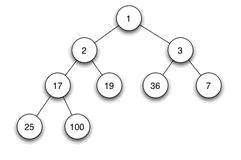
\includegraphics[width=0.4\textwidth]{pictures/heap.png}
\end{center}
\caption{小顶堆}
%\label{fig:las298}
\end{figure}

由于其它几种堆(二项式堆,斐波纳契堆等)用的较少,一般将二叉堆就简称为堆。



\section{堆的储存}
一般用数组来表示堆。

(1)以下标为“0”开始的$n$个元素的序列$\{k_0,k_1,\cdots, k_{n-1}\}$当且仅当满足下列关系时
\begin{itemize}
\item 情形1:$\begin{cases}
k_i \le k_{2i+1}\\
k_i \le k_{2i+2}
\end{cases}$,称之为最小化堆或小顶堆;
\item 情形2:$\begin{cases}
k_i \ge k_{2i}\\
k_i \ge k_{2i+1}
\end{cases}$,称之为最大化堆或大顶堆。
\end{itemize}
其中$i=0,1,2,\cdots,(n/2-1)$向下取整。


(2)以下标为“1”开始的$n$个元素的序列$\{k_1,k_2,\cdots, k_n\}$当且仅当满足下列关系时
\begin{itemize}
\item 情形1:$\begin{cases}
k_i \le k_{2i}\\
k_i \le k_{2i+1}
\end{cases}$,称之为最小化堆或小顶堆;
\item 情形2:$\begin{cases}
k_i \ge k_{2i}\\
k_i \ge k_{2i+1}
\end{cases}$,称之为最大化堆或大顶堆。
\end{itemize}
其中$i=1,2,\cdots,n/2$向下取整。


\section{堆排序的思想}
有了堆的定义,就自然过渡到堆排序了。一个无序数组,如果构造成了大顶堆,这就筛选出了这个数组的最大值,即第一项(堆顶值)。此时,我们把这个最大值取出,余下的部分继续构造成大顶堆,继续取出堆顶值,反复进行就实现了原来数组的排序。但是具体操作可以变得更为有效:排序开始,首先输出堆顶元素(因为它是最值),将堆顶元素和最后一个元素交换,这样,第$n$个位置(即最后一个位置)作为有序区,前$n-1$个位置仍是无序区,对无序区进行调整,得到堆之后,再交换堆顶和最后一个元素,这样有序区长度变为$2\cdots$不断进行此操作,将剩下的元素重新调整为堆,然后输出堆顶元素到有序区。每次交换都导致无序区$-1$,有序区$+1$。不断重复此过程直到有序区长度增长为$n-1$,排序完成。由排序过程可见,若想得到升序,则建立大顶堆,若想得到降序,则建立小顶堆。

在将堆顶元素和最后一个元素交换后形成的无序区重新构建堆也是有规律可循的。这也是堆调整的最关键部分。每个子树根都是该子树分支的最值。当堆的根元素与最后一个元素交换后,重新构建堆,实际就是将处于根位置的新元素不断与子结点比较,下沉到树中的合适位置。每次完成比较,另一支子树就不用考虑,减少$1/2$需要比较的数据量。这是堆的特性所决定的,因为每个父节点都是所处树分枝的最值,无论这个树分枝是大还是小。这是堆调整的核心要点。后面会有具体例子说明。



以上思想可归纳为两个操作:
\begin{enumerate}[(1)]
\item 根据初始数组去构造初始堆(以大顶堆为例,构建一个完全二叉树,保证所有的父结点都比它的孩子结点数值大)。初始化堆的时候是对所有的非叶子结点进行筛选。最后一个非终端元素的下标是$n/2$向下取整,所以筛选只需要从第$n/2$向下取整个元素开始,从后往前进行调整。每次都是从父结点、左孩子、右孩子中进行比较交换,交换可能会引起孩子结点不满足堆的性质,所以每次交换之后需要重新对被交换的孩子结点进行调整。
\item 每次交换第一个和最后一个元素,输出最后一个元素(最大值),然后把剩下元素重新调整为大根堆。
其中调整建堆的方法是,将根结点值与左、右子树的根结点值进行比较,若不满足堆的条件,则将左、右子树根结点值中的大者与根结点值进行交换。未被破坏的子树就不用管了,然后顺着被破坏的子树一路调整下去,直至叶子结点,就得到新的堆。(牢牢记住堆的特性,父结点是所处子树的最值。堆中有相同元素也没关系,堆的定义特性在于保证堆顶是最值。即堆只能保证堆中元素的最值。对于排序,有这点就够了。)
\end{enumerate}
当输出完最后一个元素后,这个数组已经是按照从小到大的顺序排列了。



\newpage
\section{堆排序实例}
(1)以构建大顶堆实现从小到大排序为例。建立初始的堆结构如图
\begin{figure}[h]
\begin{center}
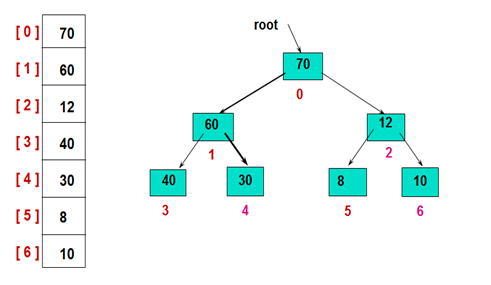
\includegraphics[width=0.5\textwidth]{pictures/2012113021435914.png}
\end{center}
%\caption{小顶堆}
%\label{fig:las298}
\end{figure}

(2)然后,交换堆顶的元素和最后一个元素,此时最后一个位置作为有序区(有序区显示为黄色)
\begin{figure}[h]
\begin{center}
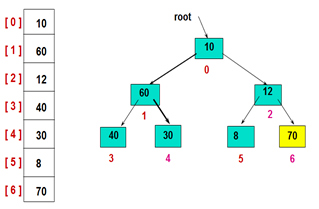
\includegraphics[width=0.5\textwidth]{pictures/heapsort1.png}
\end{center}
%\caption{小顶堆}
%\label{fig:las298}
\end{figure}

(3)每个子树根都是该子树分支的最大值。而子树根60比子树根12大,12 所在的子树无需考虑,此时一半的数据量无需比较。10比60小,60是整个序列的第二大值。交换10和60,此时筛选出了第二大值。但是为了保证余下的排序,仍要继续调整10至合适位置,直至重新构建成一个堆。
\begin{figure}[h]
\begin{center}
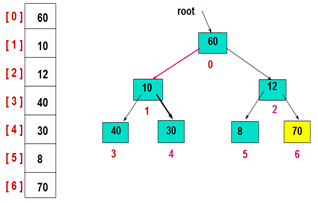
\includegraphics[width=0.5\textwidth]{pictures/heapsort2.png}
\end{center}
%\caption{小顶堆}
%\label{fig:las298}
\end{figure}

\newpage
(4)10不断下沉至合适位置,每次调整,减少余下的一半的数据去比较。此时蓝色部分重新构建称为堆。
\begin{figure}[h]
\begin{center}
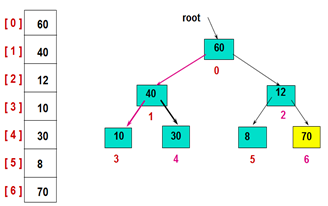
\includegraphics[width=0.5\textwidth]{pictures/heapsort3.png}
\end{center}
%\caption{小顶堆}
%\label{fig:las298}
\end{figure}

(5)进入第二轮排序,60与堆中最后一个元素交换位置。
\begin{figure}[h]
\begin{center}
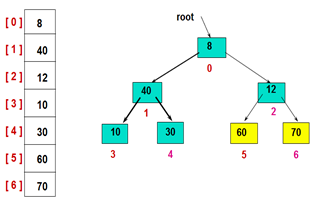
\includegraphics[width=0.5\textwidth]{pictures/heapsort4.png}
\end{center}
%\caption{小顶堆}
%\label{fig:las298}
\end{figure}


(6)又开始调整堆。
\begin{figure}[h]
\begin{center}
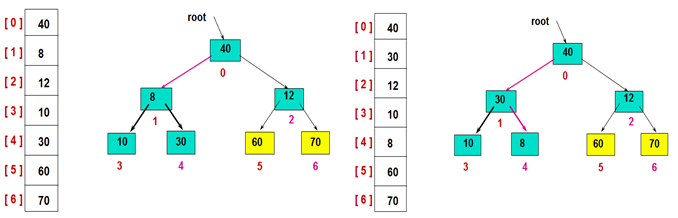
\includegraphics[width=0.9\textwidth]{pictures/heapsort5.png}
\end{center}
%\caption{小顶堆}
%\label{fig:las298}
\end{figure}

\newpage
(7)重复此过程。
\begin{figure}[h]
\begin{center}
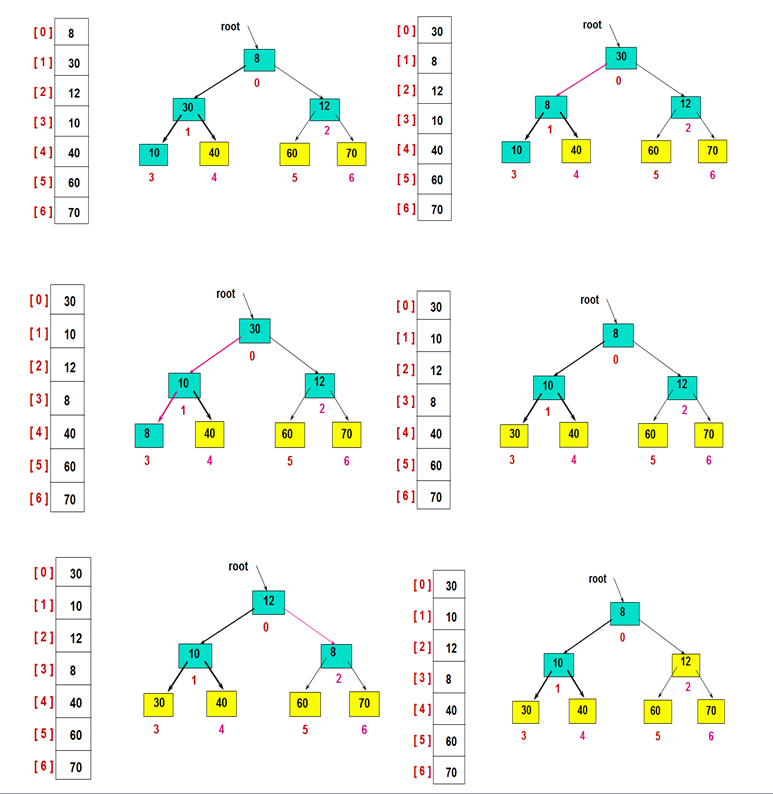
\includegraphics[width=0.75\textwidth]{pictures/2012113021474819.png}
\end{center}
%\caption{小顶堆}
%\label{fig:las298}
\end{figure}

(8)最后,有序区扩展完成即排序完成。
\begin{figure}[h]
\begin{center}
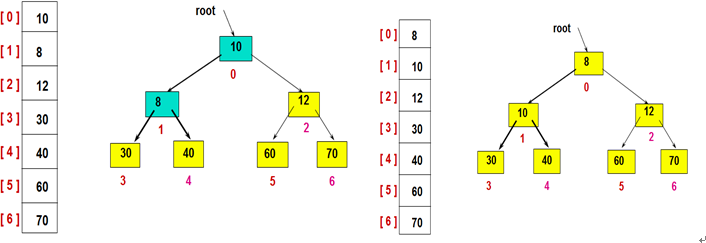
\includegraphics[width=0.75\textwidth]{pictures/2012113021482583.png}
\end{center}
%\caption{小顶堆}
%\label{fig:las298}
\end{figure}




\chapter{差分进化算法}
\section{背景}
\url{https://www.cnblogs.com/tsingke/p/5809453.html}

DE算法-作者网站: \url{http://www1.icsi.berkeley.edu/~storn/code.html}

维基百科资料库  : \url{https://en.wikipedia.org/wiki/Differential_evolution}

差分进化算法(Differential Evolution,DE)是由Storn等人于1995年提出的,和其它演化算法一样,DE是一种模拟生物进化的随机模型,通过反复迭代,使得那些适应环境的个体被保存了下来。但相比于进化算法,DE保留了基于种群的全局搜索策略,采用实数编码、基于差分的简单变异操作和一对一的竞争生存策略,降低了遗传操作的复杂性。同时,DE特有的记忆能力使其可以动态跟踪当前的搜索情况,以调整其搜索策略,具有较强的全局收敛能力和鲁棒性,且不需要借助问题的特征信息,适于求解一些利用常规的数学规划方法所无法求解的复杂环境中的优化问题。目前,DE已经在许多领域得到了应用,譬如人工神经元网络、化工、电力、机械设计、机器人、信号处理、生物信息、经济学、现代农业、食品安全、环境保护和运筹学等。
 
 
DE 算法主要用于求解连续变量的全局优化问题,其主要工作步骤与其他进化算法基本一致,主要包括变异(Mutation)、交叉(Crossover)、选择(Selection)三种操作。算法的基本思想是从某一随机产生的初始群体开始,利用从种群中随机选取的两个个体的差向量作为第三个个体的随机变化源,将差向量加权后按照一定的规则与第三个个体求和而产生变异个体,该操作称为变异。然后,变异个体与某个预先决定的目标个体进行参数混合,生成试验个体,这一过程称之为交叉。如果试验个体的适应度值优于目标个体的适应度值,则在下一代中试验个体取代目标个体,否则目标个体仍保存下来,该操作称为选择。在每一代的进化过程中,每一个体矢量作为目标个体一次,算法通过不断地迭代计算,保留优良个体,淘汰劣质个体,引导搜索过程向全局最优解逼近。


\section{具体步骤}
{\small\url{https://pablormier.github.io/2017/09/05/a-tutorial-on-differential-evolution-with-python/}}

\url{https://blog.csdn.net/qq_37423198/article/details/77856744}

\paragraph{目的} 对于一个黑箱函数,有一组参数,设参数个数为$N$。利用差分进化算法来寻找黑箱函数最小值的参数。
\begin{equation}
f(x_1,x_2,x_3,\cdots,x_N)
\end{equation}

\paragraph{定义} 将黑箱函数的一组参数称为个体;多组参数(个体)称为种群。
 
\paragraph{第〇步} 初始化种群(产生初始值):产生大小为$M$的种群,即包含$M$组参数($M$个个体)。$M$的选择一般介于参数个数$N$的5到10倍之间

\begin{itemize}
\item 设定每个参数的取值边界范围。
\begin{equation}
(b_{j-min},b_{j-max}),\quad j = 1, 2, 3, \cdots, N
\end{equation}
\item 随机产生$M$个个体($M$组参数);也可以加入自己设定的初始值。
\begin{align}
X_i(0) &= \{x_{i,1}(0),x_{i,2}(0),x_{i,3}(0),\cdots, x_{i,N}(0)\}\\
&=\begin{pmatrix}
x_{1,1}(0) & x_{1,2}(0) &x_{1,3}(0) &\cdots &x_{1,N}(0)\\
x_{2,1}(0) & x_{2,2}(0) &x_{2,3}(0) &\cdots &x_{2,N}(0)\\
x_{3,1}(0) & x_{3,2}(0) &x_{3,3}(0) &\cdots &x_{1,N}(0)\\
\vdots      &   \vdots     & \vdots      & \cdots & \vdots \\
x_{M,1}(0) & x_{M,2}(0) &x_{M,3}(0) &\cdots &x_{M,N}(0)
\end{pmatrix}
\end{align}
其中
\begin{align}
x_{i,j}(0) &= b_{j-min} + rand(0,1)* (b_{j-max}-b_{j-min})\\
 i &= 1,2,3,\cdots, M\\
 j &= 1,2,3,\cdots, N
\end{align}
\item 代入到黑箱函数计算,得出最优值。
\end{itemize}


\paragraph{第一步} 变异(按照特定策略修改参数):对之前产生的$M$个个体逐个进行变异。
\begin{itemize}
\item 变异方法:对$i$个个体进行变异,则再随机选择除第$i$个个体外的3个个体,表示为$a$、$b$、$c$,以特定的变异策略计算变异体。存在多种变异策略,以最简单的“rand1bin”为例
\begin{equation}
x_{i-mut} = a + mut * (b-c)
\end{equation}
其中$mut$是变异因子(缩放因子),取值一般在$[0.5,2]$之间。 大的变异因子可以扩大搜索范围,但是会降低收敛速度。
\item 变异策略:
\begin{itemize}
\item Rand/1: $x_{mut} = x_{r1} + mut*(x_{r2}-x_{r3})$
\item Rand/2: $x_{mut} =x_{r1} + mut*(x_{r2}-x_{r3}+x_{r4}-x_{r5})$
\item Best/1: $x_{mut}=x_{best}+mut*(x_{r2}-x_{r3})$
\item Rand-to-best/1: $x_{mut}=x_{r1}+mut_1 *(x_{r2}-x_{r3}) + mut_2*(x_{best}-x_{r1})$
\item $\cdots$
\end{itemize}
\item 自适应变异因子:暂略!
\end{itemize}



\paragraph{第二步} 交叉(将修改后的参数和原参数按照特定策略进行取舍,得到新参数):将变异体和未变异体进行混合,即将两者参数进行混合。
\begin{itemize}
\item 交叉策略:对应于每个参数,产一个随机数,将这个随机数与设定交叉因子做对比。如果小于这个因子,就保留变异体中的这个参数,否在就保留原参数。这样就实现了变异体和未变异体的混合。
\begin{equation}
x_{i,j}^{new} =\begin{cases}
x_{i,j}^{mut},& rand(0,1)\le cr\\
x_{i,j}^{ori}, &else
\end{cases}
\end{equation}

其中$cr \in [0,1]$为交叉概率。这个策略称为二项式交叉策略(Binomial crossover, bin)。还有在两组参数中随机挑选参数的指数交叉策略(Exponential crossover, exp)。

\item 自适应交叉因子:暂略!
\end{itemize}

\paragraph{第三步} 选择(对比新参数和原参数的函数值,保留最优值)


至此得到一个全新的种群。将这个全新的种群重复后三个步骤(变异、交叉、选择),进行迭代,直至找到最优解。





\chapter{数值计算库}
\section{Intel MKL}
\subsection{Intel MKL简介}
Intel数学核心函数库(Math Kernel Library, MKL)是一套高度优化、线程安全的数学例程、函数,面向高性能的工程、科学与财务应用。英特尔 MKL 的集群版本包括 ScaLAPACK 与分布式内存快速傅立叶转换,并提供了线性代数 (BLAS、LAPACK 和Sparse Solver)、快速傅立叶转换、矢量数学 (Vector Math) 与随机号码生成器支持。

主要包括:

① LAPACK (线形代数工具linear algebra package)

② DFTs (离散傅立叶变换 Discrete Fourier transforms)

③ VML (矢量数学库Vector Math Library)

④ VSL (矢量统计库Vector Statistical Library)

 
MKL的主要功能:

1)BLAS 和 LAPACK

在英特尔处理器中部署经过高度优化的基本线性代数例程BLAS(Basic Linear Algebra Subroutines)和 线性代数包LAPACK(Linear Algebra Package) 例程,它们提供的性能改善十分显著。
 
2)ScaLAPACK

ScaLAPACK是一个并行计算软件包,适用于分布存储的MIMD并行机。ScaLAPACK提供若干线性代数求解功能,具有高效、可移植、可伸缩、高可靠性的特点,利用它的求解库可以开发出基于线性代数运算的并行应用程序。
ScaLAPACK 的英特尔? MKL 实施可提供显著的性能改进,远远超出标准 NETLIB 实施所能达到的程度。
 
3)PARDISO稀疏矩阵解算器

利用 PARDISO 直接稀疏矩阵解算器解算大型的稀疏线性方程组,该解算器获得了巴塞尔大学的授权,是一款易于使用、具备线程安全性、高性能的内存高效型软件库。英特尔? MKL 还包含共轭梯度解算器和 FGMRES 迭代稀疏矩阵解算器。
 
4)快速傅立叶变换 (FFT)

充分利用带有易于使用的新型 C/Fortran 接口的多维 FFT 子程序(从 1 维至 7 维)。英特尔? MKL 支持采用相同 API 的分布式内存集群,支持将工作负载轻松地分布到大量处理器上,从而实现大幅的性能提升。此外,英特尔? MKL 还提供了一系列 C 语言例程(“wrapper”),这些例程可模拟 FFTW 2.x 和 3.0 接口,从而支持当前的 FFTW 用户将英特尔? MKL 集成到现有应用中。
 
5)矢量数学库(VML)

矢量数学库(Vector Math Library)借助计算密集型核心数学函数(幂函数、三角函数、指数函数、双曲函数、对数函数等)的矢量实施显著提升应用速度。
 
6)矢量统计库—随机数生成器(VSL)

利用矢量统计库(Vector Statistical Library)随机数生成器加速模拟,从而实现远远高于标量随机数生成器的系统性能提升。


\subsection{命名规则}
【注】这里只是简单的介绍,一切以MKL的技术手册为准,在技术手册的头几个章节就有说明。技术手册网上有,MKL安装后也有份本地文件。这个在下面的使用心得中有详细介绍。

Naming Conventions

Argument types. Types of all arguments of Fortran routines in this Quick Reference follow these conventions:
\begin{itemize}
\item IMPLICIT COMPLEX (C) 
\item IMPLICIT DOUBLE PRECISION (D) 
\item IMPLICIT INTEGER (I-N) 
\item IMPLICIT DOUBLE COMPLEX (Z) 
\item CHARACTER*1 compq, compz, diag, eigsrc, howmny, initv, job, norm, order, range, side, trans, transa, transb, uplo, vect 
LOGICAL select
\end{itemize}

Arrays. Names of Fortran arrays are typeset in UPPERCASE letters, and names of all other Fortran arguments are in lowercase letters. Code examples and data types for C interface are also given in lowercase.

Names of routines. The first letter of a routine name identifies the type of the result: 
\begin{itemize}
\item s    SINGLE 
\item d    DOUBLE PRECISION 
\item c    COMPLEX 
\item z    DOUBLE COMPLEX 
\item i    INTEGER
\end{itemize}

Function names for C interface are given in lowercase courier mixed with UpperCase courier.

To specify the group of routine names that differ in the first letter, this Quick Reference uses the question mark (?). For example, ?getrf refers to the routines sgetrf, dgetrf, cgetrf, and zgetrf.


\subsection{使用心得}
MKL用起来真的是不容易的,曲曲折折,当然了,这跟自己的Linux基础知识不够扎实有关。MKL是优化了很多现有的优秀的数学函数库。我本来想在C++直接调用这些库。后来觉得里面的BLAS原生就是用的Fortran写的,自己对Fortran熟悉,C++还不熟。所以还是一个台阶一个台阶的来吧,不然就函数接口而言估计都够折腾的,事实上Fortran 95的函数接口都折腾我够呛的。因为BLAS最初是Fortran 77写的。

先说下心得中最核心的一条:纵使你在网上搜到各种说法,万变不离其综的王道是,看MKL自带的技术手册,千多页呢,讲的不能再详细了。技术手册网上有,

\url{http://software.intel.com/sites/products/documentation/doclib/mkl_sa/11/mklman/index.htm}

安装后,本地文件也有。建议看本地文件的技术手册,与安装的版本对应,更全面,更直观。本地的技术手册,在安装目录下,Document 目录下找,所有的文档都在那。

第一天,云里雾里,什么都不知道。第二天,学会了看技术手册,是网页版的,从mkl\_documentation.htm开始。知道了命名规则,及各项参数,成功的用Fortran 77 函数接口调用了矩阵相乘的子程序。编译的时候很简单,多加个 -mkl 选项就可以了。以我的测试文件为例:\verb|ifort test1_ver1.f90 -mkl|

测试文件如下:
\lstinputlisting{program/test/test1_ver1.f90}

Fortran 95的函数接口简单,参量少,用起来方便,可是调用时屡屡出错:
\begin{verbatim}
In function `MAIN__':
test_ver2.f90:(.text+0x164): undefined reference to `dgemm_mkl95_'
\end{verbatim}

究其原因,应该是没有链接到合适的库。在mkl\_documentation.htm旁边有个
mkl\_link\_line\_advisor.htm文件,这个文件很有用。它能指出合适的链接和编译选项,只是生成链接和编译选项时,需要手动选择系统相关参数。如果系统相关参数不清楚,怎么办呢? 在 MKL的安装目录下,例如我的安装目录\verb|/opt/intel/mkl| 下有个tools目录,里面有个很有用的工具 mkl\_link\_tool。 直接运行这个程序就能得到这个程序的相关说明。如果加上参数 -check\_mkl\_presence运行,即 \verb|./mkl_link_tool -check_mkl_presence| 就能到自己安装的详细参数。用这些参数在mkl\_link\_line\_advisor.htm文件选择合适的选项,就能得到链接和编译选项,如我的:
\begin{verbatim}
Use this link line: 
$(MKLROOT)/lib/intel64/libmkl_blas95_lp64 
-L$(MKLROOT)/lib/intel64 
-lmkl_intel_lp64 -lmkl_core -lmkl_sequential -lpthread -lm

Compiler options: 
 -I$(MKLROOT)/include/intel64/lp64 -I$(MKLROOT)/include
\end{verbatim}
这里的链接和选项需要适当的调整,因为它不知道MKL的安装路径,这个要自己补充。要将\verb|$(MKLROOT)|替换成安装路径,我的安装路径为\verb|/opt/intel/mkl|。还有就是库文件libmkl\_blas95\_lp64是有后缀的,加上libmkl\_blas95\_lp64.a。这些库文件,自己可以在相应目录下看看。编译链接及编译选项都得加进去,于是最终有效的编译是:
\begin{verbatim}
ifort test1_ver2.f90 
/opt/intel/mkl/lib/intel64/libmkl_blas95_lp64.a 
-L/opt/intel/mkl/lib/intel64 
-lmkl_intel_lp64 -lmkl_core -lmkl_sequential -lpthread -lm 
-I/opt/intel/mkl/include/intel64/lp64 -I/opt/intel/mkl/include
\end{verbatim}
很长很麻烦,显然不是最终解决方案。

测试文件如下:
\lstinputlisting{program/test/test1_ver2.f90}






\section{FFTW}
\subsection{FFTW的简介}
官方网站:\url{http://www.fftw.org/}

下载地址:\url{http://www.fftw.org/download.html}

快速傅立叶变换(FFTW)是由麻省理工学院开发的免费的软件包,采用 C 语言编写,计算一维和多维离散傅立叶变换。FFTW 的编码生成器采用面向对象设计技术和面向对象语言Caml 编写;它能自动适应系统硬件,因而可移植性很强。FFTW2.1.5 支持共享存储多线程并行和分布式存储 MPI 并行。FFTW 的运算性能远远领先于目前已有的其它 FFT 软件。FFTW 为任意大小的模式生成一个计划(plan),通过对该计划施行各种运算完成各种模式的转换;内部结构及其复杂性对用户透明;速度快 (适合各种机器的内部编译器、代码生成器利用 AST 在运行时生成代码并自我优化,而且不占用编译时间,
采用分层存储技术)。FFTW 受到越来越多的科学研究和工程计算工作者的普遍青睐,并为量子物理、光谱分析、音视频流信号处理、石油勘探、地震预报、天气预报、概率论、编码理论、医学断层诊
断等领域提供切实可行的大规模 FFT 计算。


\subsection{安装调用}
(1)安装
\begin{itemize}
\item 切换到解压目录
\item 使用管理员权限 或在命令前直接加 sudo
\item ./configure
\item make
\item make check
\item make install
\end{itemize}

(2)调用

\verb*|ifort xx.f90 -lfftw3 -lm|


\subsection{实例}
在linux下有如下程序:
\begin{lstlisting}[language=Fortran]
program aab
	use fftw3
	implicit none 
	integer i , j , n
	parameter (n=8)
	type(C_PTR) :: plan
	complex(C_DOUBLE_COMPLEX), dimension(n,n) :: in, out
	do i=1,n
		do j=1,n
			in(i,j)=cmplx(cos(i*0.22),sin(j*0.3))
		enddo
	enddo
	out=0.d0
	plan =fftw_plan_dft_2d(n,n,in,out,FFTW_FORWARD,FFTW_ESTIMATE)
	call fftw_execute_dft(plan, in, out)
	write(777,*) real(out)
	write(777,*) aimag(out)
	call fftw_destroy_plan(plan)
	stop
end
\end{lstlisting}

编译 :gfotran -o x   x.f90 -lfftw3

运行:./x


\section{BLAS}
\subsection{BLAS简介}
官网:\url{http://www.netlib.org/blas/}

BLAS系Basic Linear Algebra Subprograms的缩写。顾名思义,BLAS实现基本的线性代数运算,是NetLib中一些高级软件包--比如,LAPACK和LINPACK-- 的“基石”。据说,BLAS由美国NSF和DOE资助,在1970s开始推出,至今仍在发展。这是一个PublicDomain的著名软件包。
     BLAS的基本部分由三个级别构成:第一级完成“向量-向量”操作;第二级实现“矩阵-向量”运算;第三级包含“矩阵-矩阵”程序。所有的子程序都经过精 心的优化以确保其高效性;程序的书写和语句的选择都相当规范,以便于移植。针对不同的平台,有多种经过低级别优化(比如汇编级优化)的BLAS库可供直接 使用。
     长期以来,专家们一直呼吁使用BLAS来建立和开发自己的线性代数软件包。这样做,不仅可以缩短开发周期,而且便于形成统一的调用接口。当BLAS升级 时,您可以坐享其成。由于源码是公开的,您不必担心受制于人(如果您使用商品化的IMSL或者NAG,这种担心就不是多余的)。



\section{GLS}
\url{http://blog.csdn.net/waleking/article/details/8265008/}
\subsection{GLS安装过程}
下载 gsl-1.9.tar.gz
http://ftp.club.cc.cmu.edu/pub/gnu/gsl/

安装
\begin{itemize}
\item
\verb|tar -zxvf gsl-1.9.tar.gz|
\item
\verb|cd gsl-1.9|
\item
\verb|sudo ./configure|
\item
\verb|sudo make|
\item
\verb|sudo make install|
\end{itemize}
执行最后一个命令之后会有很多现实问题,其中有:
\begin{verbatim}
Libraries have been installed in:
   /usr/local/lib

If you ever happen to want to link against installed libraries
in a given directory, LIBDIR, you must either use libtool, and
specify the full pathname of the library, or use the `-LLIBDIR'
flag during linking and do at least one of the following:
   - add LIBDIR to the `LD_LIBRARY_PATH' environment variable
     during execution
   - add LIBDIR to the `LD_RUN_PATH' environment variable
     during linking
   - use the `-Wl,--rpath -Wl,LIBDIR' linker flag
   - have your system administrator add LIBDIR to `/etc/ld.so.conf'

See any operating system documentation about shared libraries for
more information, such as the ld(1) and ld.so(8) manual pages.
\end{verbatim}
一个是\verb|libgslcblas.so|,\verb|libgsl.so|的位置很重要,编译后的文件被扔到了这里,比如 \verb|/usr/local/lib|;另一个重要的位置是
\verb|gsl_rng.h| 这样的头文件所在的文件夹目录,比如\verb|/usr/local/include/gsl|。如果想要查找他们,可以使用\verb|find / -name gsl_rng.h|这样的命令。



\subsection{使用实例}
\begin{lstlisting}[language=C]
#include <stdio.h>
#include <gsl_rng.h>
#include <gsl_randist.h>


int main (int argc, char *argv[])
{
  /* set up GSL RNG */
  gsl_rng *r = gsl_rng_alloc(gsl_rng_mt19937);
  /* end of GSL setup */


  int i,n;
  double gauss,gamma;


  n=atoi(argv[1]);
  for (i=0;i<n;i++)
    {
      gauss=gsl_ran_gaussian(r,2.0);
      gamma=gsl_ran_gamma(r,2.0,3.0);
      printf("%2.4f %2.4f\n", gauss,gamma);
    }
  return(0);
}
\end{lstlisting}

编译:

第一反应是直接 \verb|gcc gsl_test.c|

显示错误是:\verb|gsl_test.c:2: fatal error: gsl_rng.h|: 没有那个文件或目录

这个错误是说没有找到头文件,然后加上头文件的位置,

\verb|gcc -I/usr/local/include/gsl gsl_test.c|

显示错误是:\verb|gsl_test.c:(.text+0x12): undefined reference to `gsl_rng_mt19937' ...|

这个错误是说没有找到\verb|gsl_rng_mt19937|的定义,查看了\url{http://www.daniweb.com/software-development/cpp/threads/289812/cant-link-gsl-properly},这里说需要加上-lgsl,即链接到gsl,找到 libgsl.so.

使用命令:\verb|gcc -I/usr/local/include/gsl -lgsl gsl_test.c|

显示错误是:\verb|//usr/local/lib/libgsl.so: undefined reference to `cblas_ctrmv'|

查看了\url{http://sourceware.org/ml/gsl-discuss/2003-q2/msg00123.html},是说错误是由于没有链接libgslcblas.so引起的,再加上-lgslcblas可以解决问题。

使用命令:\verb|gcc -I/usr/local/include/gsl -lgsl -lgslcblas gsl_test.c|。

或者命令:\verb|gcc -I/usr/local/include/gsl -L/usr/local/lib -lgsl -lgslcblas gsl_test.c|

这个时候出现了产出物a.out。

(5)运行a.out 

./a.out 出现错误“段错误”

(6)查看源文件,发现还需要输入参数

./a.out 10

结果是:
0.2678 6.9645
3.3488 1.6894
1.9950 2.1575
-4.7934 6.1648
-0.0782 4.0292
1.7871 11.6031
-2.5931 7.7629
0.3634 1.3344
-1.0965 11.1658
0.0142 3.5412



\section{Lapack}
Lapack, Linear Algebra PACKage,是由美国国家科学基金等资助开发的,以Fortran语言编写的,开源的线性代数软件包。包含了求解科学与工程计算中最常见的数值线性代数问题,如求解线性方程组、线性最小二乘问题、特征值问题和奇异值问题等。

官网为:\url{http://www.netlib.org/lapack/},最新版可以在这里下载自行编译使用。

Lapack编译比较简单,参考下载源码中的README文件就能编译成功。但是有几点需要注意:
\begin{enumerate}[(1)]
\item 最终生成的库文件。最终生成的库文件包含三个:liblapack.a、librefblas.a、libtmglib.a,虽然可能会报几个错,但是只要三个文件生成,那基本成功了。
\item Makefile文件。Makefile文件通常不用修改。但是如下两行需要注意。如果你的系统没有安装Blas(参考前面章节),那请注释掉\verb|lib: lapacklib tmglib|这行,使用下面那行命令。反之注释第二行,使用第一行。
\begin{verbatim}
#lib: lapacklib tmglib
lib: blaslib variants lapacklib tmglib
\end{verbatim}
\item make.inc文件。make.inc文件后缀,inc是include的缩写。顾名思义,是Makefile文件的组成部分。有的开发者喜欢把需要用户自行修改的部分放在这里,而Makefile无需用户修改。有的则喜欢把需要用户自行修改的部分放在Makefile文件,而make.inc文件无需修改。这里是前者。用户需要根据自己的编译环境修改make.inc文件。如果不太懂,没关系,开发者在INSTALL文件下提供了大量的配置模板。笔者用的是ifort编译器,直接选用了make.inc.ifort。无需任何修改,直接编译成功。(当然注意把后缀改成.inc)
\item 编译。编译的时候要注意把这三个库文件都链接上。如何链接库,请看相关章节。
\end{enumerate}


\subsection{使用实例}
\begin{lstlisting}[language=Fortran]
program main
    implicit none
    INTEGER :: N, LDA, LDB
    INTEGER :: NRHS
    INTEGER :: INFO
    INTEGER :: IPIV(4)
    REAL(8) :: A(4,4), B(4,1)
    
    N=4;LDA=4;LDB=4
    NRHS=1
    
    A=reshape((/1.80,2.88,2.05,-0.89,&
                5.25,-2.95,-0.95,-3.80,&
                1.58,-2.69,-2.90,-1.04,&
                -1.11,-0.66,-0.59,0.80/),(/4,4/))
    B=reshape((/9.52,24.35,0.77,-6.22/),(/4,1/))
  
    call DGESV( N, NRHS, A, LDA, IPIV, B, LDB, INFO )
    
    write(*,*) "Solution:"
    write(*,'(f8.3)') B
    write(*,*) "INFO=", INFO
    
    stop
end program
\end{lstlisting}

编译命令:

\verb|ifort test.f90 -L/home/XX -llapack -lrefblas -ltmglib|

\verb|gfortran mred_3pe.f90 -L/home/xuanleng/Major/Core/Scripts -llapack -lrefblas|

注意写好链接库文件的目录。关于链接库文件的更多信息详看相关章节。


\section{anyschroed}









\part{Programming}
\chapter{编程日志}
2015.7.31

从今天开始,记录编程中值得记录的错误,提醒以后。

编程数值计算时,一定要注意初始化数据。当计算结果飘了,很可能是数据没有初始化导致数值累加。

最近做计算,输出结果一直为0,折腾了好几天。也由于是新编程序,担心是算法问题,各种核查很多遍,虽然侧面加深了对理论的理解,但是最终问题却跟这无关。原来是最后一步的fortran矩阵运算,matmul(um,rho1),习惯的写成了,um*rho1,导致输出为0。用的是 Intel的fortran编译器,这样的错误居然没报错,也是无语。知道Intel的fortran语法较宽松,可是这样太宽松了。所以啊,以后为了防止这类错误,还是用语法较为严格的 gfortran也编译看看吧。

2015.8.1

今天用 Intel fortran 编译程序,弹出来说许可证过期了,不能用了。哎~ 我都忘记这碴了!习惯了不为软件付费,来个这个还真不习惯。算了,以后还是用 gfortran 吧。

经常遇到如下错误:

Program received signal SIGSEGV: Segmentation fault - invalid memory reference.

一般就是数组下标过界了,一定要注意组元的赋值。

2015.8.6

Intel fortran 编译器许可证过期是个教训。不同编译器,要求不同,Intel fortran 编译器要求松些,直接导致改用 gfortran 编译器出现很多警告和计算错误。所以以后编程一定要保证这两个编译器都通过和计算一致。

商业软件就是商业软件,Intel fortran 足足比开源免费的 gfortran 快个 6 倍。




\chapter{Python}
\section{准备工作}
\subsection{安装模块}
首先安装python的模块管理器,对于python2,有\verb|sudo apt-get install python-pip|;对于python3,有\verb|sudo apt-get install python3-pip|。

安装模块,以pylab为例。对于python2,有\verb|sudo pip install pylab|;对于python3,有\verb|sudo pip3 install pylab|。

\verb|sudo apt-get install python-matplotlib|



\subsection{Ubuntu切换Python3}
因为Ubuntu很多底层采用的是Python2.*,Python3和Python2是互相不兼容的,所以此时不能卸载Python2。要使用python3.*,可以直接输入命令python3即可。输入python默认是python2.*。



\subsection{Python脚本编码设置}
在文件开头加入 \# -*- coding: UTF-8 -*- 或者 \#coding=utf-8可以设置Python脚本编码。


\subsection{设置脚本解释器的版本}
``\#!''是脚本中的约定符号,用来指定解释器的版本。
\begin{itemize}
\item 直接指定解释器路径,如:\verb|#!/usr/bin/python|、\verb|#!/usr/bin/python2.7|、
或\verb|#!/usr/bin/python3.4|

\item 通过env命令来指定解释器,如:\\

\verb|#!/usr/bin/env python|

由于在Ubuntu中Shell输入python默认调用的是python2.*,所以这是指定解释器为python2.*类版本。又如

\verb|#!/usr/bin/env python3|

由于python存在python2.*和python3.*两类版本而不兼容,所有这是指定解释器为python3.*类版本。
\end{itemize}



\subsection{脚本的执行}
对于脚本语言,执行方法都类似。类似于Shell脚本的执行一样,Python脚本的执行也有两种方法。

(1)作为解释器参数,即直接运行解释器,其参数就是Shell脚本的文件名,例如

使用Python2.*解释:
\verb|python test.py|\qquad 或更严格的 \qquad \verb|/usr/bin/python2.7 test.py|

使用Python3.*解释:
\verb|python3 test.py|\qquad 或更严格的 \qquad \verb|/usr/bin/python3.4 test.py|

这种方式运行的脚本,不需要在第一行指定解释器信息,写了也没用。

(2)作为可执行程序。

(a)在脚本所在目录下,首先使脚本具有执行权限,有两种方法:
\begin{enumerate}
\item 命令操作:\verb|chmod +x ./test.py|;
\item 图形化操作:选中脚本test.py右键勾选可以执行选项。
\end{enumerate}

(b)然后执行程序:\verb|./test.py|

注意,一定要写成./test.py,而不是test.py。这里的“./”实质指的是相对路径,即当前路径下。如果test.py在/bin目录下,当然也可以采用绝大路径来运行即“/bin/test.py”,只不过相对路径更简便些。运行其它二进制的程序也一样,直接写test.py,Linux系统会去PATH里寻找有没有叫test.py的,而只有/bin、 /sbin、 /usr/bin、/usr/sbin等在PATH里,你的当前目录通常不在PATH里,所以写成test.py是会找不到命令的,要用./test.py告诉系统说,就在当前目录找。这意味着如果你编的程序经常用,那么可以添加到系统路径中,这样就真可以直接运行了。

通过这种方式运行的脚本,第一行一定要写对,好让系统查找到正确的解释器。

这里的"系统",其实就是shell这个应用程序,但我故意写成系统,是方便理解,既然这个系统就是指shell,那么一个使用/bin/sh作为解释器的脚本是不是可以省去第一行呢?是的。



\section{Python2.*与Python3.*的主要变化}
Python的3​​.0版本,常被称为Python 3000,或简称Py3k。相对于Python的早期版本,这是一个较大的升级。为了不带入过多的累赘,Python 3.0在设计的时候没有考虑向下相容。许多针对早期Python版本设计的程式都无法在Python 3.0上正常执行。

为了照顾现有程式,Python 2.6作为一个过渡版本,基本使用了Python 2.x的语法和库,同时考虑了向Python 3.0的迁移,允许使用部分Python 3.0的语法与函数。

新的Python程序建议使用Python 3.0版本的语法。除非执行环境无法安装Python 3.0或者程式本身使用了不支援Python 3.0的第三方库。目前不支援Python 3.0的第三方库有Twisted, py2exe, PIL等。

大多数第三方库都正在努力地相容Python 3.0版本。即使无法立即使用Python 3.0,也建议编写相容Python 3.0版本的程式,然后使用Python 2.6,Python 2.7来执行。


\subsection{print语句改成print()函数}
print语句没有了,取而代之的是print()函数。 Python 2.6与Python 2.7部分地支持这种形式的print语法。在Python 2.6与Python 2.7里面,以下三种形式是等价的:
\begin{lstlisting}[language=Python]
print "fish"
print ("fish") #注意print后面有个空格
print("fish") #print()不能带有任何其它参数
\end{lstlisting}



\subsection{TypeError: `str' does not support the buffer interface}
%http://blog.csdn.net/chuanchuan608/article/details/17915959
 Python 3中套接字编程中遇到TypeError: `str' does not support the buffer interface的解决办法。

In python 3, bytes strings and unicodestrings are now two different types. Since sockets are not aware of string encodings, they are using raw bytes strings, that have a slightly differentinterface from unicode strings.
So, now, whenever you have a unicode stringthat you need to use as a byte string, you need toencode() it. And whenyou have a byte string, you need to decode it to use it as a regular(python 2.x) string.
Unicode strings are quotes enclosedstrings. Bytes strings are b"" enclosed strings




\section{基本语法}
\subsection{注释}
python注释采用 \# 开头,没有块注释。



\subsection{标识符}
\begin{itemize}
\item 标识符由字母、数字、下划线组成;

\item 所有标识符可以包括英文、数字以及下划线(\_),但不能以数字开头;

\item 标识符区分大小写;

\item 以下划线开头的标识符有特殊意义。以单下划线开头(\_foo)的代表不能直接访问的类属性,需通过类提供的接口进行访问,不能用``from xxx import *"而导入;

\item 以双下划线开头的(\_\_foo)代表类的私有成员;以双下划线开头和结尾的(\_\_foo\_\_)代表python里特殊方法专用的标识,如\_\_init\_\_()代表类的构造函数。
\end{itemize}



\subsection{保留字符}
Python中的保留字不能用作常数或变数,或任何其他标识符名称,所有Python的关键字只包含小写字母。
Python的保留字有:and、exec、not、assert、finally、or、break、for、pass、class、from、print、continue、global、
raise、def、if、return、del、import、try、elif、in、while、else、is、with、except、lambda、	yield




\subsection{缩进}
Python与其他语言最大的区别就是,Python的代码块不使用大括号(\{\})来控制类,函数以及其他逻辑判断。Python最具特色的就是用缩进来写模块。缩进的空白数量是可变的,但是所有代码块语句必须包含相同的缩进空白数量,这个必须严格执行,一般缩进4个空格。如下所示:
\begin{lstlisting}[language=Python]
if True:
    print "True"
else:
    print "False"
\end{lstlisting}
以下代码将会执行错误:
\begin{lstlisting}[language=Python]
     if True:
    print "Answer"
    print "True"
else:
    print "Answer"
  print "False"
\end{lstlisting}



\subsection{多行语句}
Python语句中一般以新行作为为语句的结束符。

但是我们可以使用斜杠( \verb|\|)将一行的语句分为多行显示,如下所示:
\begin{lstlisting}[language=Python]
 total = item_one + \ 
        item_two + \
        item_three
\end{lstlisting}

语句中包含[], \{\} 或 () 括号就不需要使用多行连接符。如下实例:
\begin{lstlisting}[language=Python]
days = ['Monday', 'Tuesday', 'Wednesday',
        'Thursday', 'Friday']
\end{lstlisting}



\subsection{引号}
Python 接收单引号(' ),双引号(" ),三引号(''' """) 来表示字符串,引号的开始与结束必须的相同类型的。

其中三引号可以由多行组成,编写多行文本的快捷语法,常用语文档字符串,在文件的特定地点,被当做注释。
\begin{lstlisting}[language=Python]
word = 'word'
sentence = "This is a sentence."
paragraph = """This is a paragraph. It is
made up of multiple lines and sentences."""
\end{lstlisting}



\subsection{空行}
函数之间或类的方法之间用空行分隔,表示一段新的代码的开始。类和函数入口之间也用一行空行分隔,以突出函数入口的开始。

空行与代码缩进不同,空行并不是Python语法的一部分。书写时不插入空行,Python解释器运行也不会出错。但是空行的作用在于分隔两段不同功能或含义的代码,便于日后代码的维护或重构。

记住:空行也是程序代码的一部分。



\subsection{同一行显示多条语句}
Python可以在同一行中使用多条语句,语句之间使用分号(;)分割,以下是一个简单的实例:
\begin{lstlisting}[language=Python]
import sys; x = 'foo'; sys.stdout.write(x + '\n')
\end{lstlisting}



\subsection{多个语句构成代码组}
缩进相同的一组语句构成一个代码块,我们称之代码组。像if、while、def和class这样的复合语句,首行以关键字开始,以冒号( : )结束,该行之后的一行或多行代码构成代码组。我们将首行及后面的代码组称为一个子句(clause)。如下实例:
\begin{lstlisting}[language=Python]
if expression : 
    suite 
elif expression :  
    suite  
else :  
    suite 
\end{lstlisting}



\section{变量赋值}
变量存储在内存中的值。这就意味着在创建变量时会在内存中开辟一个空间。基于变量的数据类型,解释器会分配指定内存,并决定什么数据可以被存储在内存中。因此,变量可以指定不同的数据类型,这些变量可以存储整数,小数或字符。

Python中的变量不需要声明,变量的赋值操作既是变量声明和定义的过程。
每个变量在内存中创建,都包括变量的标识,名称和数据这些信息。
每个变量在使用前都必须赋值,变量赋值以后该变量才会被创建。
等号(=)用来给变量赋值,等号(=)运算符左边是一个变量名,等号(=)运算符右边是存储在变量中的值。例如:
\begin{lstlisting}[language=Python]
#coding=utf-8
#!/usr/bin/python

counter = 100 # 赋值整型变量
miles = 1000.0 # 浮点型
name = "John" # 字符串

print counter
print miles
print name
\end{lstlisting}
以上实例中,100,1000.0和"John"分别赋值给counter,miles,name变量。执行以上程序会输出如下结果:
\begin{lstlisting}[language=Python]
100
1000.0
John
\end{lstlisting}

Python也允许同时为多个变量赋值。例如:
\begin{lstlisting}[language=Python]
a = b = c = 1
\end{lstlisting}
以上实例,创建一个整型对象,值为1,三个变量被分配到相同的内存空间上。

可以为多个对象指定多个变量。例如:
\begin{lstlisting}[language=Python]
a, b, c = 1, 2, "john"
\end{lstlisting}
以上实例,两个整型对象1和2的分配给变量a和b,字符串对象"john"分配给变量c。



\section{标准数据类型}
Python有五个标准的数据类型:
\begin{itemize}
\item Numbers(数字)
\item String(字符串)
\item List(列表)
\item Tuple(元组)
\item Dictionary(字典)
\end{itemize}


\subsection{数字}
数字数据类型用于存储数值。Python支持四种不同的数值类型:
\begin{itemize}
\item int(有符号整型)
\item long(长整型[也可以代表八进制和十六进制])
\item float(浮点型)
\item complex(复数)
\end{itemize}

具体使用注意事项:
\begin{itemize}
\item Python使用"L"来显示长整型,如:535633629843L。长整型也可以使用小写"L",但是还是建议您使用大写"L",避免与数字"1"混淆;

\item 浮点型可以用科学表示,如:2.1e+3表示$2.1\times 10^3=2100.0$、2.1e-3表示$2.1\times 10^{-3}=0.0021$,也可以用大写的E;

\item 复数由实数部分和虚数部分构成,可以用a + bj或者complex(a,b)表示, 复数的实部a和虚部b都是浮点型,也可以用大写的J。
\end{itemize}


\subsection{字符串}
字符串或串(String)是由数字、字母、下划线组成的一串字符。一般记为 :
\begin{lstlisting}[language=Python]
s="a1a2···an"(n>=0)
\end{lstlisting}
它是编程语言中表示文本的数据类型。

python的字串列表有2种取值顺序:
\begin{itemize}
\item 从左到右索引默认0开始的,最大范围是字符串长度少1
\item 从右到左索引默认-1开始的,最大范围是字符串开头
\end{itemize}
如果你的实要取得一段子串的话,可以用到变量[头下标:尾下标],就可以截取相应的字符串,其中下标是从0开始算起,可以是正数或负数,下标可以为空表示取到头或尾。比如:
\begin{lstlisting}[language=Python]
s = 'ilovepython'
\end{lstlisting}
s[1:5]的结果是love。当使用以冒号分隔的字符串,python返回一个新的对象,结果包含了以这对偏移标识的连续的内容,左边的开始是包含了下边界。上面的结果包含了s[1]的值l,而取到的最大范围不包括上边界,就是s[5]的值p。

加号(+)是字符串连接运算符,星号(*)是重复操作。如下实例:
\begin{lstlisting}[language=Python]
#coding=utf-8
#!/usr/bin/python

str = 'Hello World!'

print str # 输出完整字符串
print str[0] # 输出字符串中的第一个字符
print str[2:5] # 输出字符串中第三个至第五个之间的字符串
print str[2:] # 输出从第三个字符开始的字符串
print str * 2 # 输出字符串两次
print str + "TEST" # 输出连接的字符串
\end{lstlisting}
以上实例输出结果:
\begin{lstlisting}[language=Python]
Hello World!
H
llo
llo World!
Hello World!Hello World!
Hello World!TEST
\end{lstlisting}


\subsubsection{转义字符}
在需要在字符中使用特殊字符时,python用反斜杠(\verb|\|)转义字符。如下表:

\begin{tabular}{l|l}
转义字符&	描述\\
\verb|\| (在行尾时)&	续行符\\
\verb|\\|	&反斜杠符号\\
\verb|\'|	&单引号\\
\verb|\"|	&双引号\\
\verb|\a|	&响铃\\
\verb|\b|	&退格(Backspace)\\
\verb|\e|	&转义\\
\verb|\000|	&空\\
\verb|\n|	&换行\\
\verb|\v|	&纵向制表符\\
\verb|\t|	&横向制表符\\
\verb|\r|	&回车\\
\verb|\f|	&换页\\
\verb|\oyy|	&八进制数,yy代表的字符,例如:\verb|\o12|代表换行\\
\verb|\xyy|	&十六进制数,yy代表的字符,例如:\verb|\x0a|代表换行\\
\verb|\other|	&其它的字符以普通格式输出
\end{tabular}


\subsubsection{字符串运算符}
下表实例变量a值为字符串"Hello",b变量值为"Python":

\begin{itemize}
\item 操作符;	描述;	实例
\item +	;字符串连接;	a + b 输出结果: HelloPython
\item *;	重复输出字符串;	a*2 输出结果:HelloHello
\item \verb|[]|	; 通过索引获取字符串中字符;	a[1] 输出结果 e
\item \verb|[ : ]|; 	截取字符串中的一部分	a[1:4] 输出结果 ell
\item in;	成员运算符 - 如果字符串中包含给定的字符返回 True;	H in a 输出结果 1
\item not in;	成员运算符 - 如果字符串中不包含给定的字符返回 True;	M not in a 输出结果 1
\item r/R;	原始字符串 - 原始字符串:所有的字符串都是直接按照字面的意思来使用,没有转义特殊或不能打印的字符。 原始字符串除在字符串的第一个引号前加上字母"r"(可以大小写)以外,与普通字符串有着几乎完全相同的语法。;	\verb|print r'\n' prints \n| 和 \verb|print R'\n' prints \n|
\end{itemize}



\subsubsection{三引号——字符串的抄录}
python中三引号可以将复杂的字符串进行抄录,即python三引号允许一个字符串跨多行,字符串中可以包含换行符、制表符以及其他特殊字符。三引号的语法是一对连续的单引号或者双引号(通常都是成对的用)。
\begin{lstlisting}[language=Python]
>>> hi = '''hi 
... there'''
>>> hi
'hi \nthere'
>>> print(hi)
hi 
there
>>> 
\end{lstlisting}

三引号让程序员从引号和特殊字符串的泥潭里面解脱出来,自始至终保持一小块字符串的格式是所谓的WYSIWYG(所见即所得)格式的。


\subsubsection{Unicode 字符串}
Python 中定义一个 Unicode 字符串和定义一个普通字符串一样简单:
\begin{lstlisting}[language=Python]
>>> u'Hello World !'
u'Hello World !'
\end{lstlisting}

引号前小写的"u"表示这里创建的是一个 Unicode 字符串。如果你想加入一个特殊字符,可以使用 Python 的 Unicode-Escape 编码。如下例所示:
\begin{lstlisting}[language=Python]
>>> u'Hello\u0020World !'
u'Hello World !'
\end{lstlisting}
被替换的 \u0020 标识表示在给定位置插入编码值为 0x0020 的 Unicode 字符(空格符)。


\subsubsection{字符串内建函数}
 以下实例展示了capitalize()方法的实例:
\begin{lstlisting}[language=Python]
#!/usr/bin/python

str = "this is string example....wow!!!";

print "str.capitalize() : ", str.capitalize()
\end{lstlisting}
输出结果如下:
\begin{lstlisting}[language=Python]
str.capitalize() :  This is string example....wow!!!
\end{lstlisting}


\subsection{列表}
List(列表) 是 Python 中使用最频繁的数据类型。
列表可以完成大多数集合类的数据结构实现。它支持字符,数字,字符串甚至可以包含列表(所谓嵌套)。
列表用[ ]标识。是python最通用的复合数据类型。
列表中的值得分割也可以用到变量[头下标:尾下标],就可以截取相应的列表,从左到右索引默认0开始的,从右到左索引默认-1开始,下标可以为空表示取到头或尾。
加号(+)是列表连接运算符,星号(*)是重复操作。
如下实例:
\begin{lstlisting}[language=Python]
#coding=utf-8
#!/usr/bin/python

list = [ 'abcd', 786 , 2.23, 'john', 70.2 ]
tinylist = [123, 'john']

print list # 输出完整列表
print list[0] # 输出列表的第一个元素
print list[1:3] # 输出第二个至第三个的元素 
print list[2:] # 输出从第三个开始至列表末尾的所有元素
print tinylist * 2 # 输出列表两次
print list + tinylist # 打印组合的列表
\end{lstlisting}
以上实例输出结果:
\begin{lstlisting}[language=Python]
['abcd', 786, 2.23, 'john', 70.2]
abcd
[786, 2.23]
[2.23, 'john', 70.2]
[123, 'john', 123, 'john']
['abcd', 786, 2.23, 'john', 70.2, 123, 'john']
\end{lstlisting}


\subsubsection{更新列表}
可以对列表的数据项进行修改或更新,也可以使用append()方法来添加列表项,如下所示:
\begin{lstlisting}[language=Python]
#!/usr/bin/python

list = ['physics', 'chemistry', 1997, 2000];

print "Value available at index 2 : "
print list[2];
list[2] = 2001;
print "New value available at index 2 : "
print list[2];
\end{lstlisting}
输出结果:
\begin{lstlisting}[language=Python]
Value available at index 2 :
1997
New value available at index 2 :
2001
\end{lstlisting}


\subsubsection{删除列表元素}
可以使用 del 语句来删除列表的的元素,如下实例:
\begin{lstlisting}[language=Python]
#!/usr/bin/python

list1 = ['physics', 'chemistry', 1997, 2000];

print list1;
del list1[2];
print "After deleting value at index 2 : "
print list1;
\end{lstlisting}
输出结果:
\begin{lstlisting}[language=Python]
['physics', 'chemistry', 1997, 2000]
After deleting value at index 2 :
['physics', 'chemistry', 2000]
\end{lstlisting}


\subsubsection{列表操作符}
列表对 + 和 * 的操作符与字符串相似。+ 号用于组合列表,* 号用于重复列表。
如下所示:

\begin{tabular}{l|l|l}
表达式&	结果&	描述\\
\verb|len([1, 2, 3])|&	3&	长度\\
\verb|[1, 2, 3] + [4, 5, 6]|&	\verb|[1, 2, 3, 4, 5, 6]|&	组合\\
\verb|['Hi!'] * 4| &	\verb|['Hi!', 'Hi!', 'Hi!', 'Hi!']| &	重复\\
\verb|3 in [1, 2, 3]| &	True&	元素是否存在于列表中\\
\verb|for x in [1, 2, 3]: print x| &	1 2 3&	迭代
\end{tabular}


\subsubsection{列表截取}
Python的列表截取与字符串操作类型,如下所示:
\begin{lstlisting}[language=Python]
L = ['spam', 'Spam', 'SPAM!']
\end{lstlisting}
操作:

\begin{tabular}{l|l|l}
表达式&	结果&	描述\\
L[2]&	'SPAM!'	&读取列表中第三个元素\\
L[-2]&	'Spam'	&读取列表中倒数第二个元素\\
L[1:]&	['Spam', 'SPAM!']&	从第二个元素开始截取列表
\end{tabular}


\subsubsection{列表内置函数}
\begin{itemize}
\item cmp(list1, list2):
比较两个列表的元素
\item	len(list):
列表元素个数
\item	max(list):
返回列表元素最大值
\item	min(list):
返回列表元素最小值
\item	list(seq):
将元组转换为列表
\end{itemize}


\subsubsection{列表方法}
\begin{itemize}
\item list.append(obj) :在列表末尾添加新的对象

\item list.count(obj):统计某个元素在列表中出现的次数

\item list.extend(seq):在列表末尾一次性追加另一个序列中的多个值(用新列表扩展原来的列表)

\item list.index(obj):从列表中找出某个值第一个匹配项的索引位置

\item list.insert(index, obj):将对象插入列表

\item list.pop(obj=list[-1]):移除列表中的一个元素(默认最后一个元素),并且返回该元素的值

\item list.remove(obj):移除列表中某个值的第一个匹配项

\item list.reverse():反向列表中元素

\item list.sort([func]):对原列表进行排序
\end{itemize}







\subsection{元组}
Tuple(元组)是另一个数据类型,类似于List(列表)。
元组用"()"标识。内部元素用逗号隔开。但是元素不能二次赋值,相当于只读列表。
\begin{lstlisting}[language=Python]
#coding=utf-8
#!/usr/bin/python

tuple = ( 'abcd', 786 , 2.23, 'john', 70.2 )
tinytuple = (123, 'john')

print tuple # 输出完整元组
print tuple[0] # 输出元组的第一个元素
print tuple[1:3] # 输出第二个至第三个的元素 
print tuple[2:] # 输出从第三个开始至列表末尾的所有元素
print tinytuple * 2 # 输出元组两次
print tuple + tinytuple # 打印组合的元组
\end{lstlisting}
以上实例输出结果:
\begin{lstlisting}[language=Python]
('abcd', 786, 2.23, 'john', 70.2)
abcd
(786, 2.23)
(2.23, 'john', 70.2)
(123, 'john', 123, 'john')
('abcd', 786, 2.23, 'john', 70.2, 123, 'john')
\end{lstlisting}
以下是元组无效的,因为元组是不允许更新的。而列表是允许更新的:
\begin{lstlisting}[language=Python]
#coding=utf-8
#!/usr/bin/python

tuple = ( 'abcd', 786 , 2.23, 'john', 70.2 )
list = [ 'abcd', 786 , 2.23, 'john', 70.2 ]
#tuple[2] = 1000 # 元组中是非法应用
list[2] = 1000 # 列表中是合法应用
\end{lstlisting}


\subsubsection{连接元组}
元组中的元素值是不允许修改的,但我们可以对元组进行连接组合,如下实例:
\begin{lstlisting}[language=Python]
#coding=utf-8
#!/usr/bin/python

tup1 = (12, 34.56);
tup2 = ('abc', 'xyz');

# 以下修改元组元素操作是非法的。
# tup1[0] = 100;

# 创建一个新的元组
tup3 = tup1 + tup2;
print tup3;
\end{lstlisting}
输出结果:
\begin{lstlisting}[language=Python]
(12, 34.56, 'abc', 'xyz')
\end{lstlisting}


\subsubsection{删除元组}
元组中的元素值是不允许删除的,但我们可以使用del语句来删除整个元组,如下实例:
\begin{lstlisting}[language=Python]
#!/usr/bin/python

tup = ('physics', 'chemistry', 1997, 2000);

print tup;
del tup;
print "After deleting tup : "
print tup;
\end{lstlisting}
以上实例元组被删除后,输出变量会有异常信息,输出如下所示:
\begin{lstlisting}[language=Python]
('physics', 'chemistry', 1997, 2000)
After deleting tup :
Traceback (most recent call last):
  File "test.py", line 9, in <module>
    print tup;
NameError: name 'tup' is not defined
\end{lstlisting}


\subsubsection{元组运算符}
与字符串一样,元组之间可以使用 + 号和 * 号进行运算。这就意味着他们可以组合和复制,运算后会生成一个新的元组。

\begin{tabular}{l|l|l}
表达式&	结果&	描述\\
\verb|len((1, 2, 3))|&	3	&计算元素个数\\
\verb|(1, 2, 3) + (4, 5, 6)|	&\verb|(1, 2, 3, 4, 5, 6)|&	连接\\
\verb|['Hi!'] * 4|	&\verb|['Hi!', 'Hi!', 'Hi!', 'Hi!']| &	复制\\
\verb|3 in (1, 2, 3)|&	True&	元素是否存在\\
\verb|for x in (1, 2, 3): print x| &	1 2 3	&迭代
\end{tabular}


\subsubsection{元组索引、截取}
因为元组也是一个序列,所以我们可以访问元组中的指定位置的元素,也可以截取索引中的一段元素,如下所示:

元组:\verb|L = ('spam', 'Spam', 'SPAM!')|

\begin{tabular}{l|l|l}
 表达式 & 	结果&	描述\\
\verb|L[2]| &	\verb|'SPAM!'| &	读取第三个元素\\
\verb|L[-2]| &	\verb|'Spam'|	 &反向读取;读取倒数第二个元素\\
\verb|L[1:]| &	\verb|('Spam', 'SPAM!')| &	截取元素
\end{tabular}


\subsubsection{无关闭分隔符}
任意无符号的对象,以逗号隔开,默认为元组,如下实例:
\begin{lstlisting}[language=Python]
#!/usr/bin/python

print 'abc', -4.24e93, 18+6.6j, 'xyz';
x, y = 1, 2;
print "Value of x , y : ", x,y;
\end{lstlisting}
以上实例允许结果:
\begin{lstlisting}[language=Python]
abc -4.24e+93 (18+6.6j) xyz
Value of x , y : 1 2
\end{lstlisting}


\subsubsection{元组内置函数}
Python元组包含了以下内置函数:
\begin{itemize}
\item 	cmp(tuple1, tuple2):比较两个元组元素。
\item	len(tuple):计算元组元素个数。
\item	max(tuple):返回元组中元素最大值。
\item	min(tuple):返回元组中元素最小值。
\item	tuple(seq):将列表转换为元组。
\end{itemize}


\subsection{字典}
字典(dictionary)是除列表以外python之中最灵活的内置数据结构类型。列表是有序的对象结合,字典是无序的对象集合。两者之间的区别在于:字典当中的元素是通过键来存取的,而不是通过偏移存取。字典用"\{ \}"标识。字典由索引(key)和它对应的值value组成。如下示例:
\begin{lstlisting}[language=Python]
#coding=utf-8
#!/usr/bin/python

dict = {}
dict['one'] = "This is one"
dict[2] = "This is two"

tinydict = {'name': 'john','code':6734, 'dept': 'sales'}


print dict['one'] # 输出键为'one' 的值
print dict[2] # 输出键为 2 的值
print tinydict # 输出完整的字典
print tinydict.keys() # 输出所有键
print tinydict.values() # 输出所有值
\end{lstlisting}
输出结果为:
\begin{lstlisting}[language=Python]
This is one
This is two
{'code': 6734, 'name': 'john', 'dept': 'sales'}
dict_keys(['code', 'name', 'dept'])
dict_values([6734, 'john', 'sales'])
\end{lstlisting}


\subsubsection{字典键的特性}
字典值可以没有限制地取任何python对象,既可以是标准的对象,也可以是用户定义的,但键不行。

两个重要的点需要记住:

1)不允许同一个键出现两次。创建时如果同一个键被赋值两次,后一个值会被记住,如下实例:
\begin{lstlisting}[language=Python]
#!/usr/bin/python
 
dict = {'Name': 'Zara', 'Age': 7, 'Name': 'Manni'};
 
print "dict['Name']: ", dict['Name'];
\end{lstlisting}
输出结果:
\begin{lstlisting}[language=Python]
dict['Name']:  Manni
\end{lstlisting}

2)键必须不可变,所以可以用数,字符串或元组充当,所以用列表就不行,如下实例:
\begin{lstlisting}[language=Python]
#!/usr/bin/python
 
dict = {['Name']: 'Zara', 'Age': 7};
 
print "dict['Name']: ", dict['Name'];
\end{lstlisting}
输出结果:
\begin{lstlisting}[language=Python]
Traceback (most recent call last):
  File "test.py", line 3, in <module>
    dict = {['Name']: 'Zara', 'Age': 7};
TypeError: list objects are unhashable
\end{lstlisting}



\subsubsection{修改字典}
向字典添加新内容的方法是增加新的键/值对,修改或删除已有键/值对如下实例:
\begin{lstlisting}[language=Python]
#!/usr/bin/python
 
dict = {'Name': 'Zara', 'Age': 7, 'Class': 'First'};
 
dict['Age'] = 8; # update existing entry
dict['School'] = "DPS School"; # Add new entry
 
 
print "dict['Age']: ", dict['Age'];
print "dict['School']: ", dict['School'];
\end{lstlisting}
输出结果:
\begin{lstlisting}[language=Python]
dict['Age']:  8
dict['School']:  DPS School
\end{lstlisting}


\subsubsection{删除字典}
能删单一的元素也能清空字典,清空只需一项操作。

显示删除一个字典用del命令,如下实例:
\begin{lstlisting}[language=Python]
#coding=utf-8
#!/usr/bin/python
 
dict = {'Name': 'Zara', 'Age': 7, 'Class': 'First'};
 
del dict['Name']; # 删除键是'Name'的条目
dict.clear();     # 清空词典所有条目
del dict ;        # 删除词典
 
print "dict['Age']: ", dict['Age'];
print "dict['School']: ", dict['School'];
\end{lstlisting}
但这会引发一个异常,因为用del后字典不再存在:
\begin{lstlisting}[language=Python]
dict['Age']:
Traceback (most recent call last):
  File "test.py", line 8, in <module>
    print "dict['Age']: ", dict['Age'];
TypeError: 'type' object is unsubscriptable
\end{lstlisting}


\subsubsection{字典内置函数\&方法}
Python字典包含了以下内置函数:
\begin{itemize}
\item 	cmp(dict1, dict2)
比较两个字典元素。
\item len(dict)
计算字典元素个数,即键的总数。
\item	str(dict)
输出字典可打印的字符串表示。
\item	type(variable)
返回输入的变量类型,如果变量是字典就返回字典类型。
\end{itemize}


Python字典包含了以下内置方法:
\begin{itemize}
\item 	radiansdict.clear()
删除字典内所有元素
\item	radiansdict.copy()
返回一个字典的浅复制
\item	radiansdict.fromkeys()
创建一个新字典,以序列seq中元素做字典的键,val为字典所有键对应的初始值
\item	radiansdict.get(key, default=None)
返回指定键的值,如果值不在字典中返回default值
\item	radiansdict.has\_key(key)
如果键在字典dict里返回true,否则返回false
\item	radiansdict.items()
以列表返回可遍历的(键, 值) 元组数组
\item	radiansdict.keys()
以列表返回一个字典所有的键
\item	radiansdict.setdefault(key, default=None)
和get()类似, 但如果键不已经存在于字典中,将会添加键并将值设为default
\item	radiansdict.update(dict2)
把字典dict2的键/值对更新到dict里
\item	radiansdict.values()
以列表返回字典中的所有值
\end{itemize}






\subsection{数据类型转换}
数据类型的转换只需要将数据类型作为函数名即可。以下几个内置的函数可以执行数据类型之间的转换。这些函数返回一个新的对象,表示转换的值。
\begin{itemize}
\item int(x [,base]):将x转换为一个整数

\item long(x [,base] ):将x转换为一个长整数

\item float(x):将x转换到一个浮点数

\item complex(real [,imag]):创建一个复数

\item str(x):将对象 x 转换为字符串

\item repr(x):将对象 x 转换为表达式字符串

\item eval(str):用来计算在字符串中的有效Python表达式,并返回一个对象

\item tuple(s):将序列 s 转换为一个元组

\item list(s):将序列 s 转换为一个列表

\item set(s):转换为可变集合

\item dict(d):创建一个字典。d 必须是一个序列 (key,value)元组。

\item frozenset(s):转换为不可变集合

\item chr(x):将一个整数转换为一个字符

\item unichr(x):将一个整数转换为Unicode字符

\item ord(x):将一个字符转换为它的整数值

\item hex(x):将一个整数转换为一个十六进制字符串

\item oct(x):将一个整数转换为一个八进制字符串
\end{itemize}



\subsubsection{不同类型的数字}
对于初学者,各种不同的数值类型令人迷惑。请看下面4 个不同的值:5、5.0、'5'和'5.0'。虽然它们看起来相似,但内部表示截然不同。

5 是一个整数,可直接用于算术运算。5.0 是一个浮点数,也可用于算术运算,但包含小数部分。

'5' 和'5.0' 都是字符串,分别包含1个和3 个字符。字符串可显示到屏幕上或用于基于字符的操作(如删除空白或计算字符数)。字符串不能用于算术运算。当然,字符串可用于拼接,虽然结果可能让人觉得有点不合情理。例如:
\begin{lstlisting}[language=Python]
>>> 3 * '5'
'555'
>>> 3 * '5.0'
'5.05.05.0'
\end{lstlisting}



\section{输入与输出}
\subsection{读取键盘输入}
Python提供了两个内置函数从标准输入读入一行文本,默认的标准输入是键盘。如下:
\begin{itemize}
\item \verb|raw_input()|
\item \verb|input()|
\end{itemize}


\subsubsection{raw\_input函数}
\verb|raw_input([prompt])| 函数从标准输入读取一个行,并返回一个字符串,按「Enter」完成输入:
\begin{lstlisting}[language=Python]
#!/usr/bin/python
 
str = raw_input("Enter your input: ");
print "Received input is : ", str
\end{lstlisting}
这将提示你输入任意字符串,然后在屏幕上显示相同的字符串。当我输入"Hello Python!",它的输出如下:
\begin{lstlisting}[language=Python]
Enter your input: Hello Python!
Received input is :  Hello Python!
\end{lstlisting}


\subsubsection{input() 函数}
input([prompt]) 函数和raw\_input([prompt]) 函数基本可以互换,但是input会假设输入是一个有效的Python表达式,并返回运算结果。例如:
\begin{lstlisting}[language=Python]
#!/usr/bin/python
 
str = input("Enter your input: ");
print "Received input is : ", str
\end{lstlisting}
这会产生如下的对应着输入的结果:
\begin{lstlisting}[language=Python]
Enter your input: [x*5 for x in range(2,10,2)]
Recieved input is :  [10, 20, 30, 40]
\end{lstlisting}


\subsubsection{返回值的算术运算}
由于函数input()只是返回字符串,因此如果需要的是数字(如用于算术运算),就必须使用Python 的数值转换函数。例如,请看下面的程序:
\begin{lstlisting}[language=Python]
age = input('How old are you today? ')
age10 = int(age) + 10
print('In 10 years you will be ' +  str(age10) + ' years old.')
\end{lstlisting}
假设运行该程序时用户输入22,变量age 将指向字符串'22',因为Python 不会自动将看起来像数字的字符串转换为整数或浮点数。如果要将字符串用于算术运算,必须先将其转换为数字。为此,可使用函数int(s)(如果需要的是整数)或float(s)(如果需要的是浮点数)。

这里要指出的最后一个技巧是,在print 语句中,必须将变量age10(它指向一个整数) 转换为字符串,这样才能打印它。如果忘记这样做,Python 将显示错误消息,指出不能将数字与字符串相加。


\subsection{输出}
在Python2.*中,输出是print语句;而在Python3.*中输出是print()函数。这在Python2.*和Python3.*区别章节中有相关说明。这里按照Python3.*的标准来说明。

用print()在括号中加上字符串,就可以向屏幕上输出指定的文字。比如输出\verb|'hello, world'|,用代码实现如下:
\begin{lstlisting}[language=Python]
print('hello, world')
\end{lstlisting}
print()函数也可以接受多个字符串,用逗号“,”隔开,就可以连成一串输出:
\begin{lstlisting}[language=Python]
 print('The quick brown fox', 'jumps over', 'the lazy dog')
\end{lstlisting}
print()会依次打印每个字符串,遇到逗号“,”会输出一个空格,因此,输出的字符串是这样拼起来的:

\verb|The quick brown fox jumps over the lazy dog|

print()也可以打印整数,或者计算结果:
\begin{lstlisting}[language=Python]
>>> print(300)
300
>>> print(100 + 200)
300
\end{lstlisting}

考虑到print()会依次打印每个字符串,我们可以把计算100 + 200的结果打印得更漂亮一点:
\begin{lstlisting}[language=Python]
>>> print('100 + 200 =', 100 + 200)
100 + 200 = 300
\end{lstlisting}
其中,对于100 + 200,Python解释器自动计算出结果300。但是,'100 + 200 ='是字符串而非数学公式,Python把它视为字符串,直接输出。



\subsection{格式化输出}
Python中的格式化输出是以字符串的形式进行格式化输出。尽管格式化输出可能会用到非常复杂的表达式,但最基本的用法是将一个值插入到一个有字符串格式符\%s 的字符串中。在 Python 中,字符串格式化使用与 C 中 sprintf 函数一样的语法。如下实例:
\begin{lstlisting}[language=Python]
#!/usr/bin/python

print "My name is %s and weight is %d kg!" % ('Zara', 21) 
\end{lstlisting}
以上实例输出结果:
\begin{lstlisting}[language=Python]
My name is Zara and weight is 21 kg!
\end{lstlisting}

python字符串格式化符号:

\begin{tabular}{l|l}
符   号	& 描述\\
      \%c	& 格式化字符及其ASCII码\\
      \%s	& 格式化字符串\\
      \%d	& 格式化整数\\
      \%u	& 格式化无符号整型\\
      \%o	& 格式化无符号八进制数\\
      \%x	& 格式化无符号十六进制数\\
      \%X	& 格式化无符号十六进制数(大写)\\
      \%f	& 格式化浮点数字,可指定小数点后的精度\\
      \%e	& 用科学计数法格式化浮点数\\
      \%E	& 作用同\%e,用科学计数法格式化浮点数\\
      \%g	& \%f和\%e的简写\\
      \%G	& \%f 和 \%E 的简写\\
      \%p	& 用十六进制数格式化变量的地址
\end{tabular}

格式化操作符辅助指令:

\begin{tabular}{l|l}
符号&	功能\\
*	&定义宽度或者小数点精度\\
-	&用做左对齐\\
+	&在正数前面显示加号( + )\\
<sp>&	在正数前面显示空格\\
\#	&在八进制数前面显示零('0'),在十六进制前面显示'0x'或者'0X'(取决于用的是'x'还是'X')\\
0	&显示的数字前面填充'0'而不是默认的空格\\
\%	& '\%\%'输出一个单一的'\%'\\
(var)	&映射变量(字典参数)\\
m.n.	&m 是显示的最小总宽度,n 是小数点后的位数(如果可用的话)
\end{tabular}



\subsection{格式化输出举例}
使用print输出各型的
\begin{itemize}
\item 字符串
\item 整数
\item 浮点数
\item 出度及精度控制
\end{itemize}

例如:
\begin{lstlisting}[language=Python]
h=int(5.32)
print '-'%h
print 'd'%h
\end{lstlisting}
输出 ' 5',5前面有空格保持两位数;输出 '05' ,5前面有0保持两位数。
 
 \begin{lstlisting}[language=Python]
strHello = 'Hello Python' 
print strHello 
\end{lstlisting}
输出:Hello Python,直接出字符串。


\subsubsection{格式化输出整数}
python print也支持参数格式化,与C言的printf似,
 \begin{lstlisting}[language=Python]
strHello = "the length of (%s) is %d" %('Hello World',len('Hello World'))
print strHello
\end{lstlisting}
输出:the length of (Hello World) is 11


\subsubsection{格式化输出16制整数}
nHex = 0x20
\begin{itemize}
\item \%x --- hex 十六进制
\item \%d --- dec 十进制
\item \%o --- oct 八进制
\end{itemize}
 
 \begin{lstlisting}[language=Python]
print "nHex = %x,nDec = %d,nOct = %o" %(nHex,nHex,nHex)
 \end{lstlisting}
输出结果:nHex = 20,nDec = 32,nOct = 40,使用整数的各个制打印同一个数。


\subsubsection{格式化输出浮点数}
 \begin{lstlisting}[language=Python]
import math
#default
print "PI = %f" % math.pi

#width = 10,precise = 3,align = left
print "PI = .3f" % math.pi

#width = 10,precise = 3,align = rigth
print "PI = %-10.3f" % math.pi

#前面填充字符
print "PI = d" % int(math.pi)
  \end{lstlisting}
输出结果
 \begin{lstlisting}[language=Python]
PI = 3.141593
PI =      3.142
PI = 3.142
PI = 000003
  \end{lstlisting}
%浮点数的格式化,精度、度和


\subsubsection{格式化输出字符串}
 \begin{lstlisting}[language=Python]
#precise = 3
print "%.3s " % ("jcodeer")
#precise = 4
print "%.*s" % (4,"jcodeer")
#width = 10,precise = 3
print ".3s" % ("jcodeer")
  \end{lstlisting}
输出结果:
 \begin{lstlisting}[language=Python]
jco
jcod
       jco
  \end{lstlisting}
%同于字符串也存在精度、度和。



\subsection{python读入csv的三种方式}
读数据到python有好几种方法,我们以读取iris.csv为例,将其中的数值部分提取出来。

第一种方法是列表理解,文件读取到lines之后用一个嵌套的列表理解就可以将数值存为一个list。

第二种方法是使用numpy库,它内带的loadtxt函数,读取的数据都认作是字符串,所以在第二行取我们需要的部分,并转为数值array。

第三种方法是使用pandas库,它内带read\_csv函数,读取数据会自动判断数值还是字符串,而且会自动保存好变量名,只需要用ix方法就可以类似R一样取出需要的子集,它存为dataframe对象。

这三种方法中最后一种最简单,不过花费时间比较长一点,第一种最麻烦,不过用时最短。这个可以通过ipython中的magic函数timeit来看。











\section{文件及目录操作}
\begin{itemize}
\item file 对象方法: file对象提供了操作文件的一系列方法。
\item os 对象方法: 提供了处理文件及目录的一系列方法。
\end{itemize}



\subsection{打开和关闭文件}
Python提供了必要的函数和方法进行默认情况下的文件基本操作,可以用file对象做大部分的文件操作。


\subsubsection{open函数}
先用Python内置的open()函数打开一个文件,创建一个file对象,相关的辅助方法才可以调用它进行读写。语法如下:
 \begin{lstlisting}[language=Python]
file object = open(file_name [, access_mode][, buffering])
  \end{lstlisting}
各个参数的细节:
\begin{itemize}
\item \verb|file_name|:\verb|file_name|变量是一个包含了你要访问的文件名称的字符串值。

\item \verb|access_mode|:\verb|access_mode|决定了打开文件的模式:只读,写入,追加等。所有可取值见如下的完全列表。这个参数是非强制的,默认文件访问模式为只读(r)。

\item buffering:如果buffering的值被设为0,就不会有寄存。如果buffering的值取1,访问文件时会寄存行。如果将buffering的值设为大于1的整数,表明了这就是的寄存区的缓冲大小。如果取负值,寄存区的缓冲大小则为系统默认。
\end{itemize}

不同模式打开文件的完全列表:
\begin{itemize}
\item 模式:描述
\item r	:以只读方式打开文件。文件的指针将会放在文件的开头。这是默认模式。
\item rb	:以二进制格式打开一个文件用于只读。文件指针将会放在文件的开头。这是默认模式。
\item r+	:打开一个文件用于读写。文件指针将会放在文件的开头。
\item rb+	:以二进制格式打开一个文件用于读写。文件指针将会放在文件的开头。
\item w	:打开一个文件只用于写入。如果该文件已存在则将其覆盖。如果该文件不存在,创建新文件。
\item wb	:以二进制格式打开一个文件只用于写入。如果该文件已存在则将其覆盖。如果该文件不存在,创建新文件。
\item w+	:打开一个文件用于读写。如果该文件已存在则将其覆盖。如果该文件不存在,创建新文件。
\item wb+	:以二进制格式打开一个文件用于读写。如果该文件已存在则将其覆盖。如果该文件不存在,创建新文件。
\item a	:打开一个文件用于追加。如果该文件已存在,文件指针将会放在文件的结尾。也就是说,新的内容将会被写入到已有内容之后。如果该文件不存在,创建新文件进行写入。
\item ab	:以二进制格式打开一个文件用于追加。如果该文件已存在,文件指针将会放在文件的结尾。也就是说,新的内容将会被写入到已有内容之后。如果该文件不存在,创建新文件进行写入。
\item a+	:打开一个文件用于读写。如果该文件已存在,文件指针将会放在文件的结尾。文件打开时会是追加模式。如果该文件不存在,创建新文件用于读写。
\item ab+	:以二进制格式打开一个文件用于追加。如果该文件已存在,文件指针将会放在文件的结尾。如果该文件不存在,创建新文件用于读写。
\end{itemize}



\subsubsection{file 对象的属性}
一个文件被打开后,就有一个file对象,可以得到有关该文件的各种信息。以下是和file对象相关的所有属性的列表:
\begin{itemize}
\item 属性:描述
\item file.closed	:返回true如果文件已被关闭,否则返回false。
\item file.mode	:返回被打开文件的访问模式。
\item file.name	:返回文件的名称。
\item file.softspace	:如果用print输出后,必须跟一个空格符,则返回false。否则返回true。
\end{itemize}
如下实例:
 \begin{lstlisting}[language=Python]
#coding=utf-8
#!/usr/bin/python
 
# 打开一个文件
fo = open("foo.txt", "wb")
print "Name of the file: ", fo.name
print "Closed or not : ", fo.closed
print "Opening mode : ", fo.mode
print "Softspace flag : ", fo.softspace
  \end{lstlisting}
以上实例输出结果:
 \begin{lstlisting}[language=Python]
Name of the file:  foo.txt
Closed or not :  False
Opening mode :  wb
Softspace flag :  0
  \end{lstlisting}



\subsubsection{close()方法}
file对象的close()方法刷新缓冲区里任何还没写入的信息,并关闭该文件,这之后便不能再进行写入。
当一个文件对象的引用被重新指定给另一个文件时,Python会关闭之前的文件。用close()方法关闭文件是一个很好的习惯。

语法:
 \begin{lstlisting}[language=Python]
 fileobject.close();
  \end{lstlisting}

例子:
 \begin{lstlisting}[language=Python]
#coding=utf-8
#!/usr/bin/python
 
# 打开一个文件
fo = open("foo.txt", "wb")
print "Name of the file: ", fo.name
 
# 关闭打开的文件
fo.close()
  \end{lstlisting}
以上实例输出结果:
 \begin{lstlisting}[language=Python]
Name of the file:  foo.txt
  \end{lstlisting}



\subsection{读取和写入文件}
\subsubsection{write()方法}
write()方法可将任何字符串写入一个打开的文件。需要重点注意的是,Python字符串可以是二进制数据,而不是仅仅是文字。write()方法不在字符串的结尾不添加换行符('\verb|\n|')。

语法:
 \begin{lstlisting}[language=Python]
fileobject.write(string);
  \end{lstlisting}

在这里,被传递的参数是要写入到已打开文件的内容。例如:
 \begin{lstlisting}[language=Python]
#coding=utf-8
#!/usr/bin/python
 
# 打开一个文件
fo = open("/tmp/foo.txt", "wb")
fo.write( "Python is a great language.\nYeah its great!!\n");
 
# 关闭打开的文件
fo.close()
  \end{lstlisting}
上述方法会创建foo.txt文件,并将收到的内容写入该文件,并最终关闭文件。如果你打开这个文件,将看到以下内容:
 \begin{lstlisting}[language=Python]
Python is a great language.
Yeah its great!!
  \end{lstlisting}



\subsubsection{read() 方法}
read()方法从一个打开的文件中读取一个字符串。需要重点注意的是,Python字符串可以是二进制数据,而不是仅仅是文字。

语法:

 \begin{lstlisting}[language=Python]
fileobject.read([count]);
  \end{lstlisting}
在这里,被传递的参数是要从已打开文件中读取的字节计数。该方法从文件的开头开始读入,如果没有传入count,它会尝试尽可能多地读取更多的内容,很可能是直到文件的末尾。

例如:
 \begin{lstlisting}[language=Python]
#coding=utf-8
#!/usr/bin/python
 
# 打开一个文件
fo = open("/tmp/foo.txt", "r+")
str = fo.read(10);
print "Read String is : ", str
# 关闭打开的文件
fo.close()
  \end{lstlisting}

输出结果:
 \begin{lstlisting}[language=Python]
Read String is :  Python is
  \end{lstlisting}



\subsubsection{文件位置}
tell()方法告诉你文件内的当前位置;换句话说,下一次的读写会发生在文件开头这么多字节之后。

seek(offset [,from])方法改变当前文件的位置。offset变量表示要移动的字节数。from变量指定开始移动字节的参考位置。如果from被设为0,这意味着将文件的开头作为移动字节的参考位置。如果设为1,则使用当前的位置作为参考位置。如果它被设为2,那么该文件的末尾将作为参考位置。

例如:
 \begin{lstlisting}[language=Python]
#coding=utf-8
#!/usr/bin/python
 
# 打开一个文件
fo = open("/tmp/foo.txt", "r+")
str = fo.read(10);
print "Read String is : ", str
 
# 查找当前位置
position = fo.tell();
print "Current file position : ", position
 
# 把指针再次重新定位到文件开头
position = fo.seek(0, 0);
str = fo.read(10);
print "Again read String is : ", str
# 关闭打开的文件
fo.close()
  \end{lstlisting}
实例输出结果:
 \begin{lstlisting}[language=Python]
Read String is :  Python is
Current file position :  10
Again read String is :  Python is
  \end{lstlisting}



\subsection{重命名和删除文件}
Python的os模块提供了帮你执行文件处理操作的方法,比如重命名和删除文件。
要使用这个模块,你必须先导入它,然后可以调用相关的各种功能。



\subsubsection{rename()方法}
rename()方法需要两个参数,当前的文件名和新文件名。

语法:
 \begin{lstlisting}[language=Python]
os.rename(current_file_name, new_file_name)
  \end{lstlisting}

例如:下例将重命名一个已经存在的文件test1.txt。
 \begin{lstlisting}[language=Python]
#coding=utf-8
#!/usr/bin/python
import os
 
# 重命名文件test1.txt到test2.txt。
os.rename( "test1.txt", "test2.txt" )
  \end{lstlisting}



\subsubsection{remove()方法}
用remove()方法删除文件,需要提供要删除的文件名作为参数。

语法:
 \begin{lstlisting}[language=Python]
os.remove(file_name)
  \end{lstlisting}

例如:删除一个已经存在的文件test2.txt。
 \begin{lstlisting}[language=Python]
#coding=utf-8
#!/usr/bin/python
import os
 
# 删除一个已经存在的文件test2.txt
os.remove("text2.txt")
  \end{lstlisting}



\subsection{创建和删除目录}
所有文件都包含在各个不同的目录下,Python也能轻松处理。os模块有许多方法能创建,删除和更改目录。
\subsubsection{mkdir() 方法}
可以使用os模块的mkdir()方法在当前目录下创建新的目录们。你需要提供一个包含了要创建的目录名称的参数。

语法:
 \begin{lstlisting}[language=Python]
os.mkdir("newdir")
  \end{lstlisting}

例如:在当前目录下创建一个新目录test
 \begin{lstlisting}[language=Python]
#coding=utf-8
#!/usr/bin/python
import os
 
# 创建目录test
os.mkdir("test")
  \end{lstlisting}



\subsubsection{chdir() 方法}
可以用chdir()方法来改变当前的目录。chdir()方法需要的一个参数是你想设成当前目录的目录名称。

语法:
 \begin{lstlisting}[language=Python]
os.chdir("newdir")
  \end{lstlisting}

例如:
 \begin{lstlisting}[language=Python]
#coding=utf-8
#!/usr/bin/python
import os
 
# 将当前目录改为"/home/newdir"
os.chdir("/home/newdir")
  \end{lstlisting}



\subsubsection{getcwd() 方法}
getcwd()方法显示当前的工作目录。

语法:
 \begin{lstlisting}[language=Python]
os.getcwd()
  \end{lstlisting}

例如:
 \begin{lstlisting}[language=Python]
#coding=utf-8
#!/usr/bin/python
import os
 
# 给出当前的目录
os.getcwd()
  \end{lstlisting}



\subsubsection{rmdir()方法}
rmdir()方法删除目录,目录名称以参数传递。需要注意的是,在删除这个目录之前,它的所有内容应该先被清除。

语法:
 \begin{lstlisting}[language=Python]
os.rmdir('dirname')
  \end{lstlisting}

例如:
 \begin{lstlisting}[language=Python]
#coding=utf-8
#!/usr/bin/python
import os
 
# 删除”/tmp/test”目录
os.rmdir( "/tmp/test"  )
  \end{lstlisting}









\section{运算符}
Python语言支持以下类型的运算符:
\begin{itemize}
\item 算术运算符
\item 比较(关系)运算符
\item 赋值运算符
\item 逻辑运算符
\item 位运算符
\item 成员运算符
\item 身份运算符
\end{itemize}


\subsection{算术运算符}
以下假设变量a为10,变量b为20:

\begin{tabular}{l|l|l}
运算符&	描述&	实例\\
+&	加 - 两个对象相加&	a + b 输出结果 30\\
-&	减 - 得到负数或是一个数减去另一个数&	a - b 输出结果 -10\\
*&	乘 - 两个数相乘或是返回一个被重复若干次的字符串&	a * b 输出结果 200\\
/&	除 - x除以y&	b / a 输出结果 2\\
\%&	取模 - 返回除法的余数&	b\% a 输出结果 0\\
**&	幂 - 返回x的y次幂	&a**b 为10的20次方, 输出结果 100000000000000000000\\
//&	取整除 - 返回商的整数部分	&9//2 输出结果 4 , 9.0//2.0 输出结果 4.0
\end{tabular}


\subsection{比较运算符}
以下假设变量a为10,变量b为20:

\begin{tabular}{l|l|l}
运算符&	描述&	实例\\
==&	等于 - 比较对象是否相等&	(a == b) 返回 False\\
!=&	不等于 - 比较两个对象是否不相等&	(a != b) 返回 true\\
<>	&不等于 - 比较两个对象是否不相等&	(a <> b) 返回 true,这个运算符类似 != \\
>	&大于 - 返回x是否大于y&	(a > b) 返回 False\\
<	&小于 - 返回x是否小于y。所有比较运算符返回1表示真,返回0表示假。这分别与特殊的变量True和False等价。注意,这些变量名的大写&	(a < b) 返回 true\\
>=	&大于等于 - 返回x是否大于等于y&	(a >= b) 返回 False\\
<=	&小于等于 - 返回x是否小于等于y&	(a <= b) 返回 true
\end{tabular}



\subsection{赋值运算符}
\begin{tabular}{l|l|l}
运算符&	描述&	实例\\
=&	简单的赋值运算符&	c = a + b 将 a + b 的运算结果赋值为 c\\
+=&	加法赋值运算符&	c += a 等效于 c = c + a\\
-=&	减法赋值运算符&	c -= a 等效于 c = c - a\\
*=&	乘法赋值运算符&	c *= a 等效于 c = c * a\\
/=&	除法赋值运算符&	c /= a 等效于 c = c / a\\
\%=&	取模赋值运算符&	c \%= a 等效于 c = c \% a\\
**=&	幂赋值运算符&	c **= a 等效于 c = c ** a\\
//=&	取整除赋值运算符&	c //= a 等效于 c = c // a
\end{tabular}


\subsection{位运算符}
按位运算符是把数字看作二进制来进行计算的。Python中的按位运算法则如下:
以下假设变量a为60,变量b为13:

\begin{tabular}{l|l|l}
运算符&	描述&	实例\\
\& &	按位与运算符&	 (a \& b) 输出结果 12 ,二进制解释: 0000 1100\\
|&	按位或运算符&	(a | b) 输出结果 61 ,二进制解释: 0011 1101\\
%{\^} &	按位异或运算符&	(a \^ b) 输出结果 49 ,二进制解释: 0011 0001\\
$\sim$	&按位取反运算符&	($\sim$a ) 输出结果 -61 ,二进制解释: 1100 0011, 在一个有符号二进制数的补码形式\\
<<&	左移动运算符	&a << 2 输出结果 240 ,二进制解释: 1111 0000\\
>>&	右移动运算符	&a >> 2 输出结果 15 ,二进制解释: 0000 1111
\end{tabular}


\subsection{逻辑运算符}
Python语言支持逻辑运算符,以下假设变量a为10,变量b为20:

\begin{tabular}{l|l|l}
运算符&	描述&	实例\\
and&	布尔"与" - 如果x为False,x and y返回False,否则它返回y的计算值。&	(a and b) 返回 true。\\
or&	布尔"或" - 如果x是True,它返回True,否则它返回y的计算值。&	(a or b) 返回 true。\\
not	&布尔"非" - 如果x为True,返回False。如果x为False,它返回True。&	not(a and b) 返回 false。
\end{tabular}


\subsection{成员运算符}
Python还支持成员运算符,测试实例中包含了一系列的成员,包括字符串,列表或元组。

\begin{tabular}{l|l|l}
运算符&	描述&	实例\\
in&	如果在指定的序列中找到值返回True,否则返回False。	&x 在 y序列中 , 如果x在y序列中返回True。\\
not in&	如果在指定的序列中没有找到值返回True,否则返回False。	&x 不在 y序列中 , 如果x不在y序列中返回True。
\end{tabular}
以下实例演示了Python所有成员运算符的操作:
\begin{lstlisting}[language=Python]
#!/usr/bin/python

a = 10
b = 20
list = [1, 2, 3, 4, 5 ];

if ( a in list ):
   print "Line 1 - a is available in the given list"
else:
   print "Line 1 - a is not available in the given list"

if ( b not in list ):
   print "Line 2 - b is not available in the given list"
else:
   print "Line 2 - b is available in the given list"

a = 2
if ( a in list ):
   print "Line 3 - a is available in the given list"
else:
   print "Line 3 - a is not available in the given list"
\end{lstlisting}
以上实例输出结果:
\begin{lstlisting}[language=Python]
Line 1 - a is not available in the given list
Line 2 - b is not available in the given list
Line 3 - a is available in the given list
\end{lstlisting}


\subsection{身份运算符}
身份运算符用于比较两个对象的存储单元。

\begin{tabular}{l|l|l}
运算符&	描述&	实例\\
is&	is是判断两个标识符是不是引用自一个对象	&x is y, 如果 id(x) 等于 id(y) , is 返回结果 1\\
is no&t	is not是判断两个标识符是不是引用自不同对象	&x is not y, 如果 id(x) 不等于 id(y). is not 返回结果 1
\end{tabular}
以下实例演示了Python所有身份运算符的操作:
\begin{lstlisting}[language=Python]
#!/usr/bin/python

a = 20
b = 20

if ( a is b ):
   print "Line 1 - a and b have same identity"
else:
   print "Line 1 - a and b do not have same identity"

if ( id(a) == id(b) ):
   print "Line 2 - a and b have same identity"
else:
   print "Line 2 - a and b do not have same identity"

b = 30
if ( a is b ):
   print "Line 3 - a and b have same identity"
else:
   print "Line 3 - a and b do not have same identity"

if ( a is not b ):
   print "Line 4 - a and b do not have same identity"
else:
   print "Line 4 - a and b have same identity"
\end{lstlisting}
以上实例输出结果:
\begin{lstlisting}[language=Python]
Line 1 - a and b have same identity
Line 2 - a and b have same identity
Line 3 - a and b do not have same identity
Line 4 - a and b do not have same identity 
\end{lstlisting}


\subsection{运算符优先级}
以下表格列出了从最高到最低优先级的所有运算符:

\begin{tabular}{l|l}
运算符	&描述\\
**&	指数 (最高优先级)\\
~ + -&	按位翻转, 一元加号和减号 (最后两个的方法名为 +@ 和 -@)\\
* / \% //	&乘,除,取模和取整除\\
+ -&	加法减法\\
>> <<	&右移,左移运算符\\
\&	 &位 'AND'\\
\verb|^|  | &	位运算符\\
<= < > >=	&比较运算符\\
<> == !=	&等于运算符\\
= \%= /= //= -= += *= **=	&赋值运算符\\
is is not&	身份运算符\\
in not in&	成员运算符\\
not or and&	逻辑运算符
\end{tabular}


\section{条件语句}
条件语句是通过一条或多条语句的执行结果(True或者False)来决定执行的代码块。Python程序语言指定任何非0和非空(null)值为true,0 或者 null为false。编程中 if 语句用于控制程序的执行,基本形式为:
\begin{lstlisting}[language=Python]
if 判断条件:
    执行语句……
else:
    执行语句……
\end{lstlisting}
其中"判断条件"成立时(非零),则执行后面的语句,而执行内容可以多行,以缩进来区分表示同一范围。else 为可选语句,当需要在条件不成立时执行内容则可以执行相关语句,具体例子如下:
\begin{lstlisting}[language=Python]
# coding=utf8
# 例1:if 基本用法

flag = False
name = 'luren'
if name == 'python':         # 判断变量否为'python'
    flag = True          # 条件成立时设置标志为真
    print 'welcome boss'    # 并输出欢迎信息
else:
    print name              # 条件不成立时输出变量名称
\end{lstlisting}
输出结果为:
\begin{lstlisting}[language=Python]
>>> luren			# 输出结果
\end{lstlisting}

if 语句的判断条件可以用>(大于)、<(小于)、==(等于)、>=(大于等于)、<=(小于等于)来表示其关系。当判断条件为多个值是,可以使用以下形式:
\begin{lstlisting}[language=Python]
if 判断条件1:
    执行语句1……
elif 判断条件2:
    执行语句2……
elif 判断条件3:
    执行语句3……
else:
    执行语句4……
\end{lstlisting}
实例如下:
\begin{lstlisting}[language=Python]
# coding=utf8
# 例2:elif用法

num = 5     
if num == 3:            # 判断num的值
    print 'boss'        
elif num == 2:
    print 'user'
elif num == 1:
    print 'worker'
elif num < 0:           # 值小于零时输出
    print 'error'
else:
    print 'roadman'     # 条件均不成立时输出
\end{lstlisting}
输出结果为:
\begin{lstlisting}[language=Python]
>>> roadman		# 输出结果
\end{lstlisting}

由于 python 并不支持 switch 语句,所以多个条件判断,只能用 elif 来实现,如果判断需要多个条件需同时判断时,可以使用 or (或),表示两个条件有一个成立时判断条件成功;使用 and (与)时,表示只有两个条件同时成立的情况下,判断条件才成功。
\begin{lstlisting}[language=Python]
# coding=utf8
# 例3:if语句多个条件

num = 9
if num >= 0 and num <= 10:    # 判断值是否在0~10之间
    print 'hello'
>>> hello		# 输出结果

num = 10
if num < 0 or num > 10:    # 判断值是否在小于0或大于10
    print 'hello'
else:
	print 'undefine'
>>> undefine		# 输出结果

num = 8
# 判断值是否在0~5或者10~15之间
if (num >= 0 and num <= 5) or (num >= 10 and num <= 15):    
    print 'hello'
else:
    print 'undefine'
>>> undefine		# 输出结果
\end{lstlisting}
当if有多个条件时可使用括号来区分判断的先后顺序,括号中的判断优先执行,此外 and 和 or 的优先级低于>(大于)、<(小于)等判断符号,即大于和小于在没有括号的情况下会比与或要优先判断。

也可以在同一行的位置上使用if条件判断语句,如下实例:
\begin{lstlisting}[language=Python]
#!/usr/bin/python 
 
var = 100 
 
if ( var  == 100 ) : print "Value of expression is 100" 
 
print "Good bye!" 
\end{lstlisting}
以上代码执行输出结果如下:
\begin{lstlisting}[language=Python]
Value of expression is 100
Good bye!
\end{lstlisting}



\section{循环语句}
\subsection{for循环}
Python for循环可以遍历任何序列的项目,如一个列表或者一个字符串。for循环的语法格式如下:
\begin{lstlisting}[language=Python]
for iterating_var in sequence:
   statements(s)
\end{lstlisting}
实例:
\begin{lstlisting}[language=Python]
#!/usr/bin/python

for letter in 'Python':     # First Example
   print 'Current Letter :', letter

fruits = ['banana', 'apple',  'mango']
for fruit in fruits:        # Second Example
   print 'Current fruit :', fruit

print "Good bye!"
\end{lstlisting}
以上实例输出结果:
\begin{lstlisting}[language=Python]
Current Letter : P
Current Letter : y
Current Letter : t
Current Letter : h
Current Letter : o
Current Letter : n
Current fruit : banana
Current fruit : apple
Current fruit : mango
Good bye!
\end{lstlisting}

另外一种执行循环的遍历方式是通过索引,如下实例:
\begin{lstlisting}[language=Python]
#!/usr/bin/python

fruits = ['banana', 'apple',  'mango']
for index in range(len(fruits)):
   print 'Current fruit :', fruits[index]

print "Good bye!"
\end{lstlisting}
以上实例输出结果:
\begin{lstlisting}[language=Python]
Current fruit : banana
Current fruit : apple
Current fruit : mango
Good bye!
\end{lstlisting}
以上实例我们使用了内置函数 len() 和 range()。函数 len() 返回列表的长度,即元素的个数。 range返回一个序列的数。

在 python 中,for … else 表示这样的意思,for 中的语句和普通的没有区别,else 中的语句会在循环正常执行完(即 for 不是通过 break 跳出而中断的)的情况下执行,while … else 也是一样。如下实例:
\begin{lstlisting}[language=Python]
#!/usr/bin/python

for num in range(10,20):  #to iterate between 10 to 20
   for i in range(2,num): #to iterate on the factors of the number
      if num%i == 0:      #to determine the first factor
         j=num/i          #to calculate the second factor
         print '%d equals %d * %d' % (num,i,j)
         break #to move to the next number, the #first FOR
   else:                  # else part of the loop
      print num, 'is a prime number'
\end{lstlisting}
以上实例输出结果:
\begin{lstlisting}[language=Python]
10 equals 2 * 5
11 is a prime number
12 equals 2 * 6
13 is a prime number
14 equals 2 * 7
15 equals 3 * 5
16 equals 2 * 8
17 is a prime number
18 equals 2 * 9
19 is a prime number
\end{lstlisting}


\subsection{while循环}
Python 编程中 while 语句用于循环执行程序,即在某条件下,循环执行某段程序,以处理需要重复处理的相同任务。其基本形式为:
\begin{lstlisting}[language=Python]
while 判断条件:
    执行语句……
\end{lstlisting}
执行语句可以是单个语句或语句块。判断条件可以是任何表达式,任何非零、或非空(null)的值均为true。
当判断条件假false时,循环结束。
实例:
\begin{lstlisting}[language=Python]
#!/usr/bin/python

count = 0
while (count < 9):
   print 'The count is:', count
   count = count + 1

print "Good bye!"
\end{lstlisting}
以上代码执行输出结果:
\begin{lstlisting}[language=Python]
The count is: 0
The count is: 1
The count is: 2
The count is: 3
The count is: 4
The count is: 5
The count is: 6
The count is: 7
The count is: 8
Good bye!
\end{lstlisting}

如果条件判断语句永远为 true,循环将会无限的执行下去,如下实例:
\begin{lstlisting}[language=Python]
#coding=utf-8
#!/usr/bin/python

var = 1
while var == 1 :  # 该条件永远为true,循环将无限执行下去
   num = raw_input("Enter a number  :")
   print "You entered: ", num

print "Good bye!"
\end{lstlisting}
以上实例输出结果:
\begin{lstlisting}[language=Python]
Enter a number  :20
You entered:  20
Enter a number  :29
You entered:  29
Enter a number  :3
You entered:  3
Enter a number between :Traceback (most recent call last):
  File "test.py", line 5, in <module>
    num = raw_input("Enter a number :")
KeyboardInterrupt
\end{lstlisting}
注意:以上的无限循环你可以使用 CTRL+C 来中断循环。

像for循环一样,while循环也可以用else语句,else中的语句会在循环正常执行完后执行,如下:
\begin{lstlisting}[language=Python]
#!/usr/bin/python

count = 0
while count < 5:
   print count, " is  less than 5"
   count = count + 1
else:
   print count, " is not less than 5"
\end{lstlisting}
以上实例输出结果为:
\begin{lstlisting}[language=Python]
0 is less than 5
1 is less than 5
2 is less than 5
3 is less than 5
4 is less than 5
5 is not less than 5
\end{lstlisting}

类似if语句的语法,如果你的while循环体中只有一条语句,你可以将该语句与while写在同一行中, 如下所示:
\begin{lstlisting}[language=Python]
#!/usr/bin/python

flag = 1

while (flag): print 'Given flag is really true!'

print "Good bye!"
\end{lstlisting}
注意:以上的无限循环你可以使用 CTRL+C 来中断循环。


\subsection{循环嵌套}
Python 语言允许在一个循环体里面嵌入另一个循环。

Python for 循环嵌套语法:
\begin{lstlisting}[language=Python]
for iterating_var in sequence:
   for iterating_var in sequence:
      statements(s)
   statements(s)
\end{lstlisting}

Python while 循环嵌套语法:
\begin{lstlisting}[language=Python]
while expression:
   while expression:
      statement(s)
   statement(s)
\end{lstlisting}
可以在循环体内嵌入其他的循环体,如在while循环中可以嵌入for循环, 反之,你可以在for循环中嵌入while循环。

实例:

以下实例使用了嵌套循环输出2$\sim$100之间的素数:
\begin{lstlisting}[language=Python]
#coding=utf-8
#!/usr/bin/python

i = 2
while(i < 100):
   j = 2
   while(j <= (i/j)):
      if not(i%j): break
      j = j + 1
   if (j > i/j) : print i, " 是素数"
   i = i + 1

print "Good bye!"
\end{lstlisting}
以上实例输出结果:
\begin{lstlisting}[language=Python]
2 是素数
3 是素数
5 是素数
7 是素数
11 是素数
13 是素数
17 是素数
19 是素数
23 是素数
29 是素数
31 是素数
37 是素数
41 是素数
43 是素数
47 是素数
53 是素数
59 是素数
61 是素数
67 是素数
71 是素数
73 是素数
79 是素数
83 是素数
89 是素数
97 是素数
Good bye!
\end{lstlisting}


\section{循环控制语句}
\subsection{break语句}
Python break语句,就像在C语言中,打破了最小封闭for或while循环。
break语句用来终止循环语句,即循环条件没有False条件或者序列还没被完全递归完,也会停止执行循环语句。
break语句用在while和for循环中。
如果使用嵌套循环,break语句将停止执行最深层的循环,并开始执行下一行代码。

Python语言 break 语句语法:
\begin{lstlisting}[language=Python]
break
\end{lstlisting}
实例:
\begin{lstlisting}[language=Python]
#!/usr/bin/python

for letter in 'Python':     # First Example
   if letter == 'h':
      break
   print 'Current Letter :', letter
  
var = 10                    # Second Example
while var > 0:              
   print 'Current variable value :', var
   var = var -1
   if var == 5:
      break

print "Good bye!"
\end{lstlisting}
以上实例执行结果:
\begin{lstlisting}[language=Python]
Current Letter : P
Current Letter : y
Current Letter : t
Current variable value : 10
Current variable value : 9
Current variable value : 8
Current variable value : 7
Current variable value : 6
Good bye!
\end{lstlisting}


\subsection{continue语句}
Python continue 语句跳出本次循环,而break跳出整个循环。
continue 语句用来告诉Python跳过当前循环的剩余语句,然后继续进行下一轮循环。
continue语句用在while和for循环中。

Python 语言 continue 语句语法格式如下:
\begin{lstlisting}[language=Python]
continue
\end{lstlisting}
实例:
\begin{lstlisting}[language=Python]
#!/usr/bin/python

for letter in 'Python':     # First Example
   if letter == 'h':
      continue
   print 'Current Letter :', letter

var = 10                    # Second Example
while var > 0:              
   var = var -1
   if var == 5:
      continue
   print 'Current variable value :', var
print "Good bye!"
\end{lstlisting}
以上实例执行结果:
\begin{lstlisting}[language=Python]
Current Letter : P
Current Letter : y
Current Letter : t
Current Letter : o
Current Letter : n
Current variable value : 9
Current variable value : 8
Current variable value : 7
Current variable value : 6
Current variable value : 4
Current variable value : 3
Current variable value : 2
Current variable value : 1
Current variable value : 0
Good bye!
\end{lstlisting}


\subsection{pass语句}
Python pass是空语句,是为了保持程序结构的完整性。

Python 语言 pass 语句语法格式如下:
\begin{lstlisting}[language=Python]
pass
\end{lstlisting}
实例:
\begin{lstlisting}[language=Python]
#!/usr/bin/python

for letter in 'Python': 
   if letter == 'h':
      pass
      print 'This is pass block'
   print 'Current Letter :', letter

print "Good bye!"
\end{lstlisting}
以上实例执行结果:
\begin{lstlisting}[language=Python]
Current Letter : P
Current Letter : y
Current Letter : t
This is pass block
Current Letter : h
Current Letter : o
Current Letter : n
Good bye!
\end{lstlisting}



\section{函数}
函数是组织好的,可重复使用的,用来实现单一,或相关联功能的代码段。

函数能提高应用的模块性,和代码的重复利用率。你已经知道Python提供了许多内建函数,比如print()。但你也可以自己创建函数,这被叫做用户自定义函数。


\subsection{定义函数}
函数是组织好的,可重复使用的,用来实现单一,或相关联功能的代码段。

函数能提高应用的模块性,和代码的重复利用率。你已经知道Python提供了许多内建函数,比如print()。但你也可以自己创建函数,这被叫做用户自定义函数。
\begin{itemize}
\item 函数代码块以def关键词开头,后接函数标识符名称和圆括号()。
\item 任何传入参数和自变量必须放在圆括号中间。圆括号之间可以用于定义参数。
\item 函数的第一行语句可以选择性地使用文档字符串—用于存放函数说明。
\item 函数内容以冒号起始,并且缩进。
\item Return[expression]结束函数,选择性地返回一个值给调用方。不带表达式的return相当于返回 None。
\end{itemize}

语法:
\begin{lstlisting}[language=Python]
def functionname( parameters ):
   "函数_文档字符串"
   function_suite
   return [expression]
\end{lstlisting}
默认情况下,参数值和参数名称是按函数声明中定义的的顺序匹配起来的。

实例:
以下为一个简单的Python函数,它将一个字符串作为传入参数,再打印到标准显示设备上。
\begin{lstlisting}[language=Python]
def printme( str ):
   "打印传入的字符串到标准显示设备上"
   print str
   return
\end{lstlisting}


\subsection{函数调用}
定义一个函数只给了函数一个名称,指定了函数里包含的参数,和代码块结构。

这个函数的基本结构完成以后,你可以通过另一个函数调用执行,也可以直接从Python提示符执行。

如下实例调用了printme()函数:
\begin{lstlisting}[language=Python]
#coding=utf-8
#!/usr/bin/python
 
# Function definition is here
def printme( str ):
   "打印任何传入的字符串"
   print str;
   return;
 
# Now you can call printme function
printme("我要调用用户自定义函数!");
printme("再次调用同一函数");
\end{lstlisting}
输出结果:
\begin{lstlisting}[language=Python]
我要调用用户自定义函数!
再次调用同一函数
\end{lstlisting}


\subsection{函数参数}
以下是调用函数时可使用的正式参数类型:
\begin{itemize}
\item 必备参数
\item 命名参数
\item 缺省参数
\item 不定长参数
\end{itemize}


\subsubsection{必备参数}
必备参数须以正确的顺序传入函数。调用时的数量必须和声明时的一样。

调用printme()函数,你必须传入一个参数,不然会出现语法错误:
\begin{lstlisting}[language=Python]
#coding=utf-8
#!/usr/bin/python
 
#可写函数说明
def printme( str ):
   "打印任何传入的字符串"
   print str;
   return;
 
#调用printme函数
printme();
\end{lstlisting}
输出结果:
\begin{lstlisting}[language=Python]
Traceback (most recent call last):
  File "test.py", line 11, in <module>
    printme();
TypeError: printme() takes exactly 1 argument (0 given)
\end{lstlisting}


\subsubsection{命名参数}
命名参数和函数调用关系紧密,调用方用参数的命名确定传入的参数值。你可以跳过不传的参数或者乱序传参,因为Python解释器能够用参数名匹配参数值。用命名参数调用printme()函数:
\begin{lstlisting}[language=Python]
#coding=utf-8
#!/usr/bin/python
 
#可写函数说明
def printme( str ):
   "打印任何传入的字符串"
   print str;
   return;
 
#调用printme函数
printme( str = "My string");
\end{lstlisting}
输出结果:
\begin{lstlisting}[language=Python]
My string
\end{lstlisting}

下例能将命名参数顺序不重要展示得更清楚:
\begin{lstlisting}[language=Python]
#coding=utf-8
#!/usr/bin/python
 
#可写函数说明
def printinfo( name, age ):
   "打印任何传入的字符串"
   print "Name: ", name;
   print "Age ", age;
   return;
 
#调用printinfo函数
printinfo( age=50, name="miki" );
\end{lstlisting}
输出结果:
\begin{lstlisting}[language=Python]
Name:  miki
Age  50
\end{lstlisting}


\subsubsection{缺省参数}
调用函数时,缺省参数的值如果没有传入,则被认为是默认值。下例会打印默认的age,如果age没有被传入:
\begin{lstlisting}[language=Python]
#coding=utf-8
#!/usr/bin/python
 
#可写函数说明
def printinfo( name, age = 35 ):
   "打印任何传入的字符串"
   print "Name: ", name;
   print "Age ", age;
   return;
 
#调用printinfo函数
printinfo( age=50, name="miki" );
printinfo( name="miki" );
\end{lstlisting}
输出结果:
\begin{lstlisting}[language=Python]
Name:  miki
Age  50
Name:  miki
Age  35
\end{lstlisting}


\subsubsection{不定长参数}
可能需要一个函数能处理比当初声明时更多的参数。这些参数叫做不定长参数,和上述2种参数不同,声明时不会命名。基本语法如下:
\begin{lstlisting}[language=Python]
def functionname([formal_args,] *var_args_tuple ):
   "函数_文档字符串"
   function_suite
   return [expression]
\end{lstlisting}
加了星号(*)的变量名会存放所有未命名的变量参数。选择不多传参数也可。如下实例:
\begin{lstlisting}[language=Python]
#coding=utf-8
#!/usr/bin/python
 
# 可写函数说明
def printinfo( arg1, *vartuple ):
   "打印任何传入的参数"
   print "输出: "
   print arg1
   for var in vartuple:
      print var
   return;
 
# 调用printinfo 函数
printinfo( 10 );
printinfo( 70, 60, 50 );
\end{lstlisting}
输出结果:
\begin{lstlisting}[language=Python]
输出:
10
输出:
70
60
50
\end{lstlisting}


\subsection{匿名函数}
用lambda关键词能创建小型匿名函数。这种函数得名于省略了用def声明函数的标准步骤。
\begin{itemize}
\item Lambda函数能接收任何数量的参数但只能返回一个表达式的值,同时只能不能包含命令或多个表达式。
\item 匿名函数不能直接调用print,因为lambda需要一个表达式。
\item lambda函数拥有自己的名字空间,且不能访问自有参数列表之外或全局名字空间里的参数。
\item 虽然lambda函数看起来只能写一行,却不等同于C或C++的内联函数,后者的目的是调用小函数时不占用栈内存从而增加运行效率。
\end{itemize}
如下实例:
\begin{lstlisting}[language=Python]
#coding=utf-8
#!/usr/bin/python
 
#可写函数说明
sum = lambda arg1, arg2: arg1 + arg2;
 
#调用sum函数
print "Value of total : ", sum( 10, 20 )
print "Value of total : ", sum( 20, 20 )
\end{lstlisting}
输出结果:
\begin{lstlisting}[language=Python]
Value of total :  30
Value of total :  40
\end{lstlisting}


\subsection{return语句}
return语句[表达式]退出函数,选择性地向调用方返回一个表达式。不带参数值的return语句返回None。之前的例子都没有示范如何返回数值,下例便告诉你怎么做:
\begin{lstlisting}[language=Python]
#coding=utf-8
#!/usr/bin/python
 
# 可写函数说明
def sum( arg1, arg2 ):
   # 返回2个参数的和."
   total = arg1 + arg2
   print "Inside the function : ", total
   return total;
 
# 调用sum函数
total = sum( 10, 20 );
print "Outside the function : ", total 
\end{lstlisting}
输出结果:
\begin{lstlisting}[language=Python]
Inside the function :  30
Outside the function :  30
\end{lstlisting}


\subsection{局部和全局变量}
一个程序的所有的变量并不是在哪个位置都可以访问的。访问权限决定于这个变量是在哪里赋值的。

变量的作用域决定了在哪一部分程序你可以访问哪个特定的变量名称。两种最基本的变量作用域如下:
全局变量、局部变量

定义在函数内部的变量拥有一个局部作用域,定义在函数外的拥有全局作用域。

局部变量只能在其被声明的函数内部访问,而全局变量可以在整个程序范围内访问。调用函数时,所有在函数内声明的变量名称都将被加入到作用域中。如下实例:
\begin{lstlisting}[language=Python]
#coding=utf-8
#!/usr/bin/python
 
total = 0; # This is global variable.
# 可写函数说明
def sum( arg1, arg2 ):
   #返回2个参数的和."
   total = arg1 + arg2; # total在这里是局部变量.
   print "Inside the function local total : ", total
   return total;
 
#调用sum函数
sum( 10, 20 );
print "Outside the function global total : ", total 
\end{lstlisting}
输出结果:
\begin{lstlisting}[language=Python]
Inside the function local total :  30
Outside the function global total :  0
\end{lstlisting}





\subsection{数学常量}
\begin{tabular}{l|l}
常量&	描述\\
pi	&数学常量 pi(圆周率,一般以π来表示)\\
e	&数学常量 e,e即自然常数(自然常数)
\end{tabular}



\subsection{数学函数——math模块}
\begin{tabular}{l|l}
函数&	返回值 ( 描述 )\\
abs(x)&	返回数字的绝对值,如abs(-10) 返回 10\\
cmp(x, y)&	如果 x < y 返回 -1, 如果 x == y 返回 0, 如果 x > y 返回 1\\
max(x1, x2,...)&	返回给定参数的最大值,参数可以为序列。\\
min(x1, x2,...)&	返回给定参数的最小值,参数可以为序列。\\
modf(x)&	返回x的整数部分与小数部分,两部分的数值符号与x相同,整数部分以浮点型表示。\\
pow(x, y)&	x**y 运算后的值。\\
round(x [,n])&	返回浮点数x的四舍五入值,如给出n值,则代表舍入到小数点后的位数。\\
ceil(x)	&返回数字的上入整数,如math.ceil(4.1) 返回 5\\
floor(x)	&返回数字的下舍整数,如math.floor(4.9)返回 4\\
exp(x)	&返回e的x次幂(ex),如math.exp(1) 返回2.718281828459045\\
log10(x)&	返回以10为基数的x的对数,如math.log10(100)返回 2.0\\
log(x)	&如math.log(math.e)返回1.0,math.log(100,10)返回2.0\\
fabs(x)	&返回数字的绝对值,如math.fabs(-10) 返回10.0\\
sqrt(x)&	返回数字x的平方根,数字可以为负数,返回类型为实数,如math.sqrt(4)返回 2+0j
\end{tabular}

其中有些需要导入math模块,通过静态对象调用该方法,如ceil()用法:
\begin{lstlisting}[language=Python]
import math

math.ceil( x )
\end{lstlisting}


三角函数

\begin{tabular}{l|l}
函数	&描述\\
acos(x)	&返回x的反余弦弧度值。\\
asin(x)	&返回x的反正弦弧度值。\\	
atan(x)	&返回x的反正切弧度值。\\
atan2(y, x)&	返回给定的 X 及 Y 坐标值的反正切值。\\
cos(x)&	返回x的弧度的余弦值。\\
hypot(x, y)&	返回欧几里德范数 sqrt(x*x + y*y)。\\
sin(x)&	返回的x弧度的正弦值。\\
tan(x)	&返回x弧度的正切值。\\
degrees(x)&	将弧度转换为角度,如degrees(math.pi/2) , 返回90.0\\
radians(x)	&将角度转换为弧度
\end{tabular}




\subsection{随机数函数——random模块}
随机数可以用于数学,游戏,安全等领域中,还经常被嵌入到算法中,用以提高算法效率,并提高程序的安全性。

Python包含以下常用随机数函数:
\begin{itemize}
\item choice(seq):	从序列的元素中随机挑选一个元素,比如random.choice(range(10)),从0到9中随机挑选一个整数。
\item randrange ([start,] stop [,step]):	从指定范围内,按指定基数递增的集合中获取一个随机数,基数缺省值为1
\item random():	随机生成下一个实数,它在[0,1)范围内。
\item seed([x]):	改变随机数生成器的种子seed。如果你不了解其原理,你不必特别去设定seed,Python会帮你选择seed。
\item shuffle(lst):	将序列的所有元素随机排序
\item uniform(x, y):	随机生成下一个实数,它在[x,y]范围内。
\end{itemize}

注意:这些函数都不能直接访问,需要导入 random 模块,然后通过 random 静态对象调用该方法。






\section{模块}
模块让你能够有逻辑地组织你的Python代码段。
把相关的代码分配到一个 模块里能让你的代码更好用,更易懂。
模块也是Python对象,具有随机的名字属性用来绑定或引用。
简单地说,模块就是一个保存了Python代码的文件。模块能定义函数,类和变量。模块里也能包含可执行的代码。

例如:
一个叫做aname的模块里的Python代码一般都能在一个叫aname.py的文件中找到。下例是个简单的模块hello.py。
\begin{lstlisting}[language=Python]
def print_func( par ):
   print "Hello : ", par
   return
\end{lstlisting}



\subsection{import语句}
想使用Python源文件,只需在另一个源文件里执行import语句,语法如下:
\begin{lstlisting}[language=Python]
import module1[, module2[,... moduleN]
\end{lstlisting}
当解释器遇到import语句,如果模块在当前的搜索路径就会被导入。搜索路径是一个解释器会先进行搜索的所有目录的列表。如想要导入模块hello.py,需要把命令放在脚本的顶端:

\begin{lstlisting}[language=Python]
#coding=utf-8
#!/usr/bin/python
 
# 导入模块
import hello
 
# 现在可以调用模块里包含的函数了
hello.print_func("Zara")
\end{lstlisting}
以上实例输出结果:
\begin{lstlisting}[language=Python]
Hello : Zara
\end{lstlisting}
一个模块只会被导入一次,不管你执行了多少次import。这样可以防止导入模块被一遍又一遍地执行。



\subsection{from…import 语句}
Python的from语句让你从模块中导入一个指定的部分到当前命名空间中。语法如下:
\begin{lstlisting}[language=Python]
from modname import name1[, name2[, ... nameN]]
\end{lstlisting}
例如,要导入模块fib的fibonacci函数,使用如下语句:
\begin{lstlisting}[language=Python]
from fib import fibonacci
\end{lstlisting}
这个声明不会把整个fib模块导入到当前的命名空间中,它只会将fib里的fibonacci单个引入到执行这个声明的模块的全局符号表。



\subsection{from…import* 语句}
使用如下声明,可以把一个模块的所有内容全都导入到当前的命令空间:
\begin{lstlisting}[language=Python]
from modname import *
\end{lstlisting}
这提供了一个简单的方法来导入一个模块中的所有项目。然而这种声明不该被过多地使用。



\subsection{定位模块}
当你导入一个模块,Python解析器对模块位置的搜索顺序是:
\begin{itemize}
\item 当前目录
\item 如果不在当前目录,Python则搜索在shell变量PYTHONPATH下的每个目录
\item 如果都找不到,Python会察看默认路径。UNIX下,默认路径一般为/usr/local/lib/python/
\end{itemize}
模块搜索路径存储在system模块的sys.path变量中。变量里包含当前目录,PYTHONPATH和由安装过程决定的默认目录。



\subsection{PYTHONPATH 变量}
作为环境变量,PYTHONPATH由装在一个列表里的许多目录组成。PYTHONPATH的语法和shell变量PATH的一样。

在Windows系统,典型的PYTHONPATH如下:
\begin{lstlisting}[language=Python]
set PYTHONPATH=c:\python20\lib;
\end{lstlisting}

在UNIX系统,典型的PYTHONPATH如下:
\begin{lstlisting}[language=Python]
set PYTHONPATH=/usr/local/lib/python
\end{lstlisting}



\subsection{命名空间和作用域}
变量是拥有匹配对象的名字(标识符)。命名空间是一个包含了变量名称们(键)和它们各自相应的对象们(值)的字典。

一个Python表达式可以访问局部命名空间和全局命名空间里的变量。如果一个局部变量和一个全局变量重名,则局部变量会覆盖全局变量。

每个函数都有自己的命名空间。类的方法的作用域规则和通常函数的一样。

Python会智能地猜测一个变量是局部的还是全局的,它假设任何在函数内赋值的变量都是局部的。

因此,如果要给全局变量在一个函数里赋值,必须使用global语句。

global VarName的表达式会告诉Python, VarName是一个全局变量,这样Python就不会在局部命名空间里寻找这个变量了。

例如,我们在全局命名空间里定义一个变量money。我们再在函数内给变量money赋值,然后Python会假定money是一个局部变量。然而,我们并没有在访问前声明一个局部变量money,结果就是会出现一个UnboundLocalError的错误。取消global语句的注释就能解决这个问题。
\begin{lstlisting}[language=Python]
#coding=utf-8
#!/usr/bin/python
 
Money = 2000
def AddMoney():
   # 想改正代码就取消以下注释:
   # global Money
   Money = Money + 1
 
print Money
AddMoney()
print Money
\end{lstlisting}



\subsection{dir()函数}
dir()函数一个排好序的字符串列表,内容是一个模块里定义过的名字。

返回的列表容纳了在一个模块里定义的所有模块,变量和函数。如下一个简单的实例:
\begin{lstlisting}[language=Python]
#coding=utf-8
#!/usr/bin/python
 
# 导入内置math模块
import math
 
content = dir(math)
 
print content;
\end{lstlisting}
以上实例输出结果:
\begin{lstlisting}[language=Python]
['__doc__', '__file__', '__name__', 'acos', 'asin', 'atan', 
'atan2', 'ceil', 'cos', 'cosh', 'degrees', 'e', 'exp', 
'fabs', 'floor', 'fmod', 'frexp', 'hypot', 'ldexp', 'log',
'log10', 'modf', 'pi', 'pow', 'radians', 'sin', 'sinh', 
'sqrt', 'tan', 'tanh']
\end{lstlisting}
在这里,特殊字符串变量\verb|__name__|指向模块的名字,\verb|__file__|指向该模块的导入文件名。



\subsection{globals()和locals()函数}
根据调用地方的不同,globals()和locals()函数可被用来返回全局和局部命名空间里的名字。

如果在函数内部调用locals(),返回的是所有能在该函数里访问的命名。

如果在函数内部调用globals(),返回的是所有在该函数里能访问的全局名字。

两个函数的返回类型都是字典。所以名字们能用keys()函数摘取。



\subsection{reload() 函数}
当一个模块被导入到一个脚本,模块顶层部分的代码只会被执行一次。

因此,如果你想重新执行模块里顶层部分的代码,可以用reload()函数。该函数会重新导入之前导入过的模块。语法如下:
\begin{lstlisting}[language=Python]
reload(module_name)
\end{lstlisting}
在这里,module\_name要直接放模块的名字,而不是一个字符串形式。比如想重载hello模块,如下:
\begin{lstlisting}[language=Python]
reload(hello)
\end{lstlisting}



\subsection{ Python中的包}
包是一个分层次的文件目录结构,它定义了一个由模块及子包,和子包下的子包等组成的Python的应用环境。包的存在可以让我们一次性导入一个目录下的所有函数。

考虑一个在Phone目录下的pots.py文件。这个文件有如下源代码:
\begin{lstlisting}[language=Python]
#coding=utf-8
#!/usr/bin/python
 
def Pots():
   print "I'm Pots Phone"
\end{lstlisting}
同样地,我们有另外两个保存了不同函数的文件:
\begin{itemize}
\item Phone/Isdn.py 含有函数Isdn()
\item Phone/G3.py 含有函数G3()
\end{itemize}
现在,在Phone目录下创建\verb|__init__.py|:
\begin{lstlisting}[language=Python]
Phone/__init__.py
\end{lstlisting}

当要导入Phone时,为了能够使用所有函数,你需要在\verb|__init__.py|里使用显式的导入语句,如下:
\begin{lstlisting}[language=Python]
from Pots import Pots
from Isdn import Isdn
from G3 import G3
\end{lstlisting}
把这些代码添加到\verb|__init__.py|之后,导入Phone包的时候这些类就全都是可用的了。
\begin{lstlisting}[language=Python]
#coding=utf-8
#!/usr/bin/python
 
# Now import your Phone Package.
import Phone
 
Phone.Pots()
Phone.Isdn()
Phone.G3()
\end{lstlisting}
以上实例输出结果:
\begin{lstlisting}[language=Python]
I'm Pots Phone
I'm 3G Phone
I'm ISDN Phone
\end{lstlisting}
如上,为了举例,我们只在每个文件里放置了一个函数,但其实可以放置许多函数。你也可以在这些文件里定义Python的类,然后为这些类建一个包。




\section{面向对象}
\subsection{面向对象技术简介}
\begin{itemize}
\item 类(Class): 用来描述具有相同的属性和方法的对象的集合。它定义了该集合中每个对象所共有的属性和方法。对象是类的实例。
\item 类变量:类变量在整个实例化的对象中是公用的。类变量定义在类中且在函数体之外。类变量通常不作为实例变量使用。
\item 数据成员:类变量或者实例变量用于处理类及其实例对象的相关的数据。
\item 方法重载:如果从父类继承的方法不能满足子类的需求,可以对其进行改写,这个过程叫方法的覆盖(override),也称为方法的重载。
\item 实例变量:定义在方法中的变量,只作用于当前实例的类。
\item 继承:即一个派生类(derived class)继承基类(base class)的字段和方法。继承也允许把一个派生类的对象作为一个基类对象对待。例如,有这样一个设计:一个Dog类型的对象派生自Animal类,这是模拟"是一个(is-a)"关系(例图,Dog是一个Animal)。
\item 实例化:创建一个类的实例,类的具体对象。
\item 方法:类中定义的函数。
\item 对象:通过类定义的数据结构实例。对象包括两个数据成员(类变量和实例变量)和方法。
\end{itemize}



\subsection{创建类}
使用class语句来创建一个新类,class之后为类的名称并以冒号结尾,如下实例:
\begin{lstlisting}[language=Python]
class ClassName:
   '类的帮助信息'   #类文档字符串
   class_suite  #类体
\end{lstlisting}
类的帮助信息可以通过ClassName.\_\_doc\_\_查看。class\_suite 由类成员,方法,数据属性组成。



\subsubsection{实例}
以下是一个简单的Python类实例:
\begin{lstlisting}[language=Python]
#coding=utf-8
class Employee:
   '所有员工的基类'
   empCount = 0

   def __init__(self, name, salary):
      self.name = name
      self.salary = salary
      Employee.empCount += 1
   
   def displayCount(self):
     print "Total Employee %d" % Employee.empCount

   def displayEmployee(self):
      print "Name : ", self.name,  ", Salary: ", self.salary
\end{lstlisting}
\begin{itemize}
\item empCount变量是一个类变量,它的值将在这个类的所有实例之间共享。你可以在内部类或外部类使用Employee.empCount访问;

\item 第一种方法\_\_init\_\_()方法是一种特殊的方法,被称为类的构造函数或初始化方法,当创建了这个类的实例时就会调用该方法。
\end{itemize}



\subsubsection{创建实例对象}
要创建一个类的实例,你可以使用类的名称,并通\_\_init\_\_方法接受参数。
\begin{lstlisting}[language=Python]
"创建 Employee 类的第一个对象"
emp1 = Employee("Zara", 2000)
"创建 Employee 类的第二个对象"
emp2 = Employee("Manni", 5000)
\end{lstlisting}



\subsubsection{访问属性}
可以使用点(.)来访问对象的属性。使用如下类的名称访问类变量:
\begin{lstlisting}[language=Python]
emp1.displayEmployee()
emp2.displayEmployee()
print "Total Employee %d" % Employee.empCount
\end{lstlisting}



\subsubsection{完整实例}
\begin{lstlisting}[language=Python]
#coding=utf-8
#!/usr/bin/python

class Employee:
   '所有员工的基类'
   empCount = 0

   def __init__(self, name, salary):
      self.name = name
      self.salary = salary
      Employee.empCount += 1
   
   def displayCount(self):
     print "Total Employee %d" % Employee.empCount

   def displayEmployee(self):
      print "Name : ", self.name,  ", Salary: ", self.salary

"创建 Employee 类的第一个对象"
emp1 = Employee("Zara", 2000)
"创建 Employee 类的第二个对象"
emp2 = Employee("Manni", 5000)
emp1.displayEmployee()
emp2.displayEmployee()
print "Total Employee %d" % Employee.empCount
\end{lstlisting}

执行以上代码输出结果如下:
\begin{lstlisting}[language=Python]
Name :  Zara ,Salary:  2000
Name :  Manni ,Salary:  5000
Total Employee 2
\end{lstlisting}

可以添加,删除,修改类的属性,如下所示:
\begin{lstlisting}[language=Python]
emp1.age = 7  # 添加一个 'age' 属性
emp1.age = 8  # 修改 'age' 属性
del emp1.age  # 删除 'age' 属性
\end{lstlisting}

也可以使用以下函数的方式来访问属性:
\begin{itemize}
\item getattr(obj, name[, default]):访问对象的属性。
\item hasattr(obj,name) :检查是否存在一个属性。
\item setattr(obj,name,value) :设置一个属性。如果属性不存在,会创建一个新属性。
\item delattr(obj, name) :删除属性。
\end{itemize}

\begin{lstlisting}[language=Python]
hasattr(emp1, 'age')    # 如果存在 'age' 属性返回 True。
getattr(emp1, 'age')    # 返回 'age' 属性的值
setattr(emp1, 'age', 8) # 添加属性 'age' 值为 8
delattr(empl, 'age')    # 删除属性 'age'
\end{lstlisting}



\subsubsection{Python内置类属性}
\begin{itemize}
\item \_\_dict\_\_ : 类的属性(包含一个字典,由类的数据属性组成);
\item \_\_doc\_\_ :类的文档字符串;
\item \_\_name\_\_:类名;
\item \_\_module\_\_:类定义所在的模块(类的全名是'\_\_main\_\_.className',如果类位于一个导入模块mymod中,那么className.\_\_module\_\_ 等于 mymod);
\item \_\_bases\_\_ :类的所有父类构成元素(包含了以个由所有父类组成的元组)。
\end{itemize}
Python内置类属性调用实例如下:
\begin{lstlisting}[language=Python]
#coding=utf-8
#!/usr/bin/python

class Employee:
   '所有员工的基类'
   empCount = 0

   def __init__(self, name, salary):
      self.name = name
      self.salary = salary
      Employee.empCount += 1
   
   def displayCount(self):
     print "Total Employee %d" % Employee.empCount

   def displayEmployee(self):
      print "Name : ", self.name,  ", Salary: ", self.salary

print "Employee.__doc__:", Employee.__doc__
print "Employee.__name__:", Employee.__name__
print "Employee.__module__:", Employee.__module__
print "Employee.__bases__:", Employee.__bases__
print "Employee.__dict__:", Employee.__dict__
\end{lstlisting}
执行以上代码输出结果如下:
\begin{lstlisting}[language=Python]
Employee.__doc__: 所有员工的基类
Employee.__name__: Employee
Employee.__module__: __main__
Employee.__bases__: ()
Employee.__dict__: {'__module__': '__main__', 'displayCount': <function displayCount at 0x10a939c80>, 'empCount': 0, 'displayEmployee': <function displayEmployee at 0x10a93caa0>, '__doc__': '\xe6\x89\x80\xe6\x9c\x89\xe5\x91\x98\xe5\xb7\xa5\xe7\x9a\x84\xe5\x9f\xba\xe7\xb1\xbb', '__init__': <function __init__ at 0x10a939578>}
\end{lstlisting}



\subsubsection{Python对象销毁(垃圾回收)}
同Java语言一样,Python使用了引用计数这一简单技术来追踪内存中的对象。在Python内部记录着所有使用中的对象各有多少引用。一个内部跟踪变量,称为一个引用计数器。当对象被创建时, 就创建了一个引用计数, 当这个对象不再需要时, 也就是说, 这个对象的引用计数变为0 时, 它被垃圾回收。但是回收不是"立即"的, 由解释器在适当的时机,将垃圾对象占用的内存空间回收。
\begin{lstlisting}[language=Python]
a = 40      # 创建对象  <40>
b = a       # 增加引用, <40> 的计数
c = [b]     # 增加引用.  <40> 的计数

del a       # 减少引用 <40> 的计数
b = 100     # 减少引用 <40> 的计数
c[0] = -1   # 减少引用 <40> 的计数
\end{lstlisting}

垃圾回收机制不仅针对引用计数为0的对象,同样也可以处理循环引用的情况。循环引用指的是,两个对象相互引用,但是没有其他变量引用他们。这种情况下,仅使用引用计数是不够的。Python 的垃圾收集器实际上是一个引用计数器和一个循环垃圾收集器。作为引用计数的补充, 垃圾收集器也会留心被分配的总量很大(及未通过引用计数销毁的那些)的对象。 在这种情况下, 解释器会暂停下来, 试图清理所有未引用的循环。

实例

析构函数 \_\_del\_\_ ,\_\_del\_\_在对象消逝的时候被调用,当对象不再被使用时,\_\_del\_\_方法运行:
\begin{lstlisting}[language=Python]
#coding=utf-8
#!/usr/bin/python

class Point:
   def __init( self, x=0, y=0):
      self.x = x
      self.y = y
   def __del__(self):
      class_name = self.__class__.__name__
      print class_name, "destroyed"

pt1 = Point()
pt2 = pt1
pt3 = pt1
print id(pt1), id(pt2), id(pt3) # 打印对象的id
del pt1
del pt2
del pt3
\end{lstlisting}
实例运行结果如下:
\begin{lstlisting}[language=Python]
3083401324 3083401324 3083401324
Point destroyed
\end{lstlisting}
注意:通常需要在单独的文件中定义一个类。



\subsubsection{类的继承}
面向对象的编程带来的主要好处之一是代码的重用,实现这种重用的方法之一是通过继承机制。继承完全可以理解成类之间的类型和子类型关系。

需要注意的地方:继承语法 class 派生类名(基类名)://... 基类名写作括号里,基本类是在类定义的时候,在元组之中指明的。

在python中继承中的一些特点:
\begin{itemize}
\item 1:在继承中基类的构造(\_\_init\_\_()方法)不会被自动调用,它需要在其派生类的构造中亲自专门调用。
\item 2:在调用基类的方法时,需要加上基类的类名前缀,且需要带上self参数变量。区别于在类中调用普通函数时并不需要带上self参数
\item 3:Python总是首先查找对应类型的方法,如果它不能在派生类中找到对应的方法,它才开始到基类中逐个查找。(先在本类中查找调用的方法,找不到才去基类中找)。
\end{itemize}
如果在继承元组中列了一个以上的类,那么它就被称作"多重继承" 。

语法:

派生类的声明,与他们的父类类似,继承的基类列表跟在类名之后,如下所示:
\begin{lstlisting}[language=Python]
class SubClassName (ParentClass1[, ParentClass2, ...]):
   'Optional class documentation string'
   class_suite
\end{lstlisting}

实例:

\begin{lstlisting}[language=Python]
#coding=utf-8
#!/usr/bin/python

class Parent:        # 定义父类
   parentAttr = 100
   def __init__(self):
      print "调用父类构造函数"

   def parentMethod(self):
      print '调用父类方法'

   def setAttr(self, attr):
      Parent.parentAttr = attr

   def getAttr(self):
      print "父类属性 :", Parent.parentAttr

class Child(Parent): # 定义子类
   def __init__(self):
      print "调用子类构造方法"

   def childMethod(self):
      print '调用子类方法 child method'

c = Child()          # 实例化子类
c.childMethod()      # 调用子类的方法
c.parentMethod()     # 调用父类方法
c.setAttr(200)       # 再次调用父类的方法
c.getAttr()          # 再次调用父类的方法
\end{lstlisting}

以上代码执行结果如下:
\begin{lstlisting}[language=Python]
调用子类构造方法
调用子类方法 child method
调用父类方法
父类属性 : 200
\end{lstlisting}

可以继承多个类
\begin{lstlisting}[language=Python]
class A:        # 定义类 A
.....

class B:         # 定义类 B
.....

class C(A, B):   # 继承类 A 和 B
.....
\end{lstlisting}

可以使用issubclass()或者isinstance()方法来检测:
\begin{itemize}
\item issubclass() - 布尔函数判断一个类是另一个类的子类或者子孙类,语法:issubclass(sub,sup);
\item isinstance(obj, Class) 布尔函数如果obj是Class类的实例对象或者是一个Class子类的实例对象则返回true。
\end{itemize}



\subsubsection{方法重写}
如果你的父类方法的功能不能满足你的需求,你可以在子类重写你父类的方法:

实例:
\begin{lstlisting}[language=Python]
#coding=utf-8
#!/usr/bin/python

class Parent:        # 定义父类
   def myMethod(self):
      print '调用父类方法'

class Child(Parent): # 定义子类
   def myMethod(self):
      print '调用子类方法'

c = Child()          # 子类实例
c.myMethod()         # 子类调用重写方法
\end{lstlisting}

执行以上代码输出结果如下:
\begin{lstlisting}[language=Python]
调用子类方法
\end{lstlisting}



\subsubsection{基础重载方法}
下表列出了一些通用的功能,可以在自己的类重写:

\begin{itemize}
\item \_\_init\_\_ ( self [,args...] ):构造函数。简单的调用方法:obj = className(args)

\item  \_\_del\_\_( self ) :析构方法,删除一个对象。简单的调用方法 : dell obj

\item	\_\_repr\_\_( self ):转化为供解释器读取的形式。简单的调用方法 : repr(obj)

\item	\_\_str\_\_( self ):用于将值转化为适于人阅读的形式。简单的调用方法 : str(obj)

\item	\_\_cmp\_\_( self, x ):对象比较。简单的调用方法 : cmp(obj, x)
\end{itemize}



\subsubsection{运算符重载}
Python同样支持运算符重载,实例如下:
\begin{lstlisting}[language=Python]
#!/usr/bin/python

class Vector:
   def __init__(self, a, b):
      self.a = a
      self.b = b

   def __str__(self):
      return 'Vector (%d, %d)' % (self.a, self.b)
   
   def __add__(self,other):
      return Vector(self.a + other.a, self.b + other.b)

v1 = Vector(2,10)
v2 = Vector(5,-2)
print v1 + v2
\end{lstlisting}
以上代码执行结果如下所示:
\begin{lstlisting}[language=Python]
Vector(7,8)
\end{lstlisting}



\subsubsection{类属性与方法}
\begin{itemize}
\item 类的私有属性,\_\_private\_attrs:两个下划线开头,声明该属性为私有,不能在类地外部被使用或直接访问。在类内部的方法中使用时 self.\_\_private\_attrs。

\item 类的方法,在类地内部,使用def关键字可以为类定义一个方法,与一般函数定义不同,类方法必须包含参数self,且为第一个参数

\item 类的私有方法,\_\_private\_method:两个下划线开头,声明该方法为私有方法,不能在类地外部调用。在类的内部调用 slef.\_\_private\_methods
\end{itemize}

实例
\begin{lstlisting}[language=Python]
#coding=utf-8
#!/usr/bin/python

class JustCounter:
	__secretCount = 0  # 私有变量
	publicCount = 0    # 公开变量

	def count(self):
		self.__secretCount += 1
		self.publicCount += 1
		print self.__secretCount

counter = JustCounter()
counter.count()
counter.count()
print counter.publicCount
print counter.__secretCount  # 报错,实例不能访问私有变量
\end{lstlisting}

Python 通过改变名称来包含类名:
\begin{lstlisting}[language=Python]
1
2
2
Traceback (most recent call last):
  File "test.py", line 17, in <module>
    print counter.__secretCount  # 报错,实例不能访问私有变量
AttributeError: JustCounter instance has no attribute '__secretCount'
\end{lstlisting}

Python不允许实例化的类访问私有数据,但你可以使用 object.\_className\_\_attrName 访问属性,将如下代码替换以上代码的最后一行代码:
\begin{lstlisting}[language=Python]
.........................
print counter._JustCounter__secretCount
\end{lstlisting}

执行以上代码,执行结果如下:
\begin{lstlisting}[language=Python]
1
2
2
2
\end{lstlisting}


\section{模块学习}
\subsection{optparse模块}
Python 有两个内建的模块用于处理命令行参数:
一个是 getopt,《Deep in python》一书中也有提到,只能简单处理 命令行参数;
另一个是 optparse,它功能强大,而且易于使用,可以方便地生成标准的、符合Unix/Posix 规范的命令行说明。

简单流程

首先,必须 import OptionParser 类,创建一个 OptionParser 对象:
\begin{lstlisting}[language=Python]
from optparse import OptionParser  
parser = OptionParser() 
\end{lstlisting}

然后,使用 add\_option 来定义命令行参数:
\begin{lstlisting}[language=Python]
parser.add_option("-f", "--file", action = "store", type = "string", dest = "fileName")
\end{lstlisting}

add\_option()参数说明:

\begin{itemize}
\item short option string: 为第一个参数,表示option的缩写,例如-f;
\item long option string: 为第二个参数,表示option的全拼,例如--file;
\end{itemize}
后面的参数皆为命名参数,命名参数为可选参数;
\begin{itemize}
\item
action=: 表示对此option的处理方式,默认值为store,表示存储option的值到解析后的options对象的成员中。action还可以有其他的值:对于bool值,使用store\_true来默认存储true,使用store\_false来默认存储false,store\_const用来存储const设置的值到此option,append表示增加option的参数到list中,此时此option是一个list,可能包含多个值,count表示对counter增加一,callback表示调用指定的函数。所有的action值如下:
store + store\_true + store\_false + store\_const + append + count + callback
\item
type=:表示此option的值的类型,默认为string,可以指定为string,int,choice, float andcomplex;
\item 
dest=:表示此option在经过optionparser解析后的options对象中成员的名字,默认使用long option string;
\item 
default=:表示比option的默认值;
\item 
metavar=:表示显示到help中option的默认值(显示到help的时候并不是default);
\item 
const=:当action为store\_const的时候,需要设置此值;
\item 
choices=:当设置type为choices时,需要设置此值;
\end{itemize}



\subsection{os模块}
一、os模块概述

Python os模块包含普遍的操作系统功能。如果你希望你的程序能够与平台无关的话,这个模块是尤为重要的。(一语中的)

二、常用方法

1、os.name

输出字符串指示正在使用的平台。如果是window 则用“nt”表示,对于Linux/Unix用户,它是“posix”。

2、os.getcwd()

函数得到当前工作目录,即当前Python脚本工作的目录路径。

3、os.listdir()

返回指定目录下的所有文件和目录名。
\begin{lstlisting}[language=Python]
>>> os.listdir(os.getcwd())
['Django', 'DLLs', 'Doc', 'include', 'Lib', 'libs', 'LICENSE.txt', 'MySQL-python-wininst.log', 'NEWS.txt', 'PIL-wininst.log', 'python.exe', 'pythonw.exe', 'README.txt', 'RemoveMySQL-python.exe', 'RemovePIL.exe', 'Removesetuptools.exe', 'Scripts', 'setuptools-wininst.log', 'tcl', 'Tools', 'w9xpopen.exe']
>>> 
\end{lstlisting}

4、os.remove()

删除一个文件。

5、os.system()

运行shell命令。
\begin{lstlisting}[language=Python]
>>> os.system('dir')
or
>>> os.system('cmd') #启动dos
\end{lstlisting}

6、os.sep 可以取代操作系统特定的路径分割符。

7、os.linesep字符串给出当前平台使用的行终止符
\begin{lstlisting}[language=Python]
>>> os.linesep
'\r\n'            #Windows使用'\r\n',Linux使用'\n'而Mac使用'\r'。
>>> os.sep
'\\'              #Windows
>>> 
\end{lstlisting}

8、os.path.split()

函数返回一个路径的目录名和文件名
\begin{lstlisting}[language=Python]
>>> os.path.split('C:\\Python25\\abc.txt')
('C:\\Python25', 'abc.txt')
\end{lstlisting}

9、os.path.isfile()和os.path.isdir()函数分别检验给出的路径是一个文件还是目录。
\begin{lstlisting}[language=Python]
>>> os.path.isdir(os.getcwd())
True
>>> os.path.isfile('a.txt')
False
\end{lstlisting}

10、os.path.exists()函数用来检验给出的路径是否真地存在
\begin{lstlisting}[language=Python]
>>> os.path.exists('C:\\Python25\\abc.txt')
False
>>> os.path.exists('C:\\Python25')
True
>>> 
\end{lstlisting}

11、os.path.abspath(name):获得绝对路径

12、os.path.normpath(path):规范path字符串形式

13、os.path.getsize(name):获得文件大小,如果name是目录返回0L

14、os.path.splitext():分离文件名与扩展名
\begin{lstlisting}[language=Python]
>>> os.path.splitext('a.txt')
('a', '.txt')
\end{lstlisting}

15、os.path.join(path,name):连接目录与文件名或目录
\begin{lstlisting}[language=Python]
>>> os.path.join('c:\\Python','a.txt')
'c:\\Python\\a.txt'
>>> os.path.join('c:\\Python','f1')
'c:\\Python\\f1'
>>> 
\end{lstlisting}

16、os.path.basename(path):返回文件名
\begin{lstlisting}[language=Python]
>>> os.path.basename('a.txt')
'a.txt'
>>> os.path.basename('c:\\Python\\a.txt')
'a.txt'
>>> 
\end{lstlisting}

17、os.path.dirname(path):返回文件路径
\begin{lstlisting}[language=Python]
>>> os.path.dirname('c:\\Python\\a.txt')
'c:\\Python'
\end{lstlisting}



\subsection{sys模块}
(1)sys.argv
很多人会想,我如何给我的程序在外部传递参数呢?这个,就可以实现。如:
\begin{lstlisting}[language=Python]
Tesy.py
Import sys
Print sys.argv[number]
\end{lstlisting}
一般情况下,number为0是这个脚本的名字,1,2…则为命令行下传递的参数,如:

Test.py脚本内容:
\begin{lstlisting}[language=Python]
import sys
 
print sys.argv[0]
print sys.argv[1]
print sys.argv[2]
print sys.argv[3]
\end{lstlisting}
那么
\begin{lstlisting}[language=Python]
[root@databak scripts]# python test.py arg1 arg2 arg3
test.py
arg1
arg2
arg3
\end{lstlisting}

一个有用的实例:
\begin{lstlisting}[language=Python]
#!/usr/bin/env python

import sys

if len(sys.argv) == 3:
	ftype = sys.argv[1]
	fname =  sys.argv[2]
else:
	print " Claculates the average of 2DES time-domain outputs."
	print " USAGE: aver filetype filename"
	print "    eg: aver rp fort.71"
	sys.exit(2)

print ftype
print fname
\end{lstlisting}


(2) sys.exit(n)
执行至主程序的末尾时,解释器会自动退出. 但是如果需要中途退出程序, 你可以调用sys.exit 函数, 它带有一个可选的整数参数返回给调用它的程序. 这意味着你可以在主程序中捕获对sys.exit 的调用。(注:0是正常退出,其他为不正常,可抛异常事件供捕获!)


(3)sys.path
大家对模块都有一定了解吧?大家在使用模块的某一个功能前,是不是需要导入呢?答案是需要。那import,\_\_import\_\_命令就不用提干嘛的了吧。那大家在执行import module\_name的时候,python内部发生了什么呢?简单的说,就是搜索module\_name。根据sys.path的路径来搜索module.name
\begin{lstlisting}[language=Python]
>>> sys.path
['', '/usr/local/lib/python24.zip', '/usr/local/lib/python2.4', '/usr/local/lib/python2.4/plat-freebsd4', '/usr/local/lib/python2.4/lib-tk', '/usr/local/lib/python2.4/lib-dynload', '/usr/local/lib/python2.4/site-packages']
\end{lstlisting}
大家以后写好的模块就可以放到上面的某一个目录下,便可以正确搜索到了。当然大家也可以添加自己的模块路径:
\begin{lstlisting}[language=Python]
Sys.path.append(“mine module path”)
\end{lstlisting}



\section{Python 内置特殊函数}
这些函数很具python特性,可以让代码更加简洁。

1、filter(function, sequence):
\begin{lstlisting}[language=Python]
str = ['a', 'b','c', 'd']

def fun1(s): return s if s != 'a' else None

ret = filter(fun1, str)

print ret

## ['b', 'c', 'd']
\end{lstlisting}
对sequence中的item依次执行function(item),将执行结果为True的item组成一个List/String/Tuple(取决于sequence的类型)返回。

可以看作是过滤函数。


 2、map(function, sequence) 
\begin{lstlisting}[language=Python]
str = ['a', 'b','c', 'd'] 

def fun2(s): return s + ".txt"

ret = map(fun2, str)

print ret

## ['a.txt', 'b.txt', 'c.txt', 'd.txt']
\end{lstlisting}
对sequence中的item依次执行function(item),见执行结果组成一个List返回:

map也支持多个sequence,这就要求function也支持相应数量的参数输入:
\begin{lstlisting}[language=Python]
def add(x, y): return x+y 
 print map(add, range(10), range(10)) 
##[0, 2, 4, 6, 8, 10, 12, 14, 16, 18]
\end{lstlisting}

3、reduce(function, sequence, starting\_value):def add1(x,y): return x + y
\begin{lstlisting}[language=Python]
print reduce(add1, range(1, 100))

print reduce(add1, range(1, 100), 20)

## 4950 (注:1+2+...+99)
## 4970 (注:1+2+...+99+20)

对sequence中的item顺序迭代调用function,如果有starting_value,还可以作为初始值调用,例如可以用来对List求和: 
\end{lstlisting}

4、lambda:
\begin{lstlisting}[language=Python]
g = lambda s: s + ".fsh"

print g("haha")

print (lambda x: x * 2) (3)

## haha.fsh

## 6
\end{lstlisting}
这是Python支持一种有趣的语法,它允许你快速定义单行的最小函数,类似与C语言中的宏,这些叫做lambda的函数.



\section{Python 数值计算库NumPy和SciPy}
标准的Python中用列表(list)保存一组值,可以用来当作数组使用。但由于列表的元素可以是任何对象,因此列表中所保存的是对象的指针。这样为了保存一个简单的列表[1,2,3],需要有三个指针和三个整数对象。对于数值运算来说这种结构显然比较浪费内存和CPU计算时间。

此外Python还提供了array模块,它所提供的array对象和列表不同,能直接保存数值,和C语言的一维数组类似。但是由于它不支持多维数组,也没有各种运算函数,因此也不适合做数值运算。

NumPy为Python提供了快速的多维数组处理的能力,而SciPy则在NumPy基础上添加了众多的科学计算所需的各种工具包,有了这两个库,Python就有几乎和Matlab一样的处理数据和计算的能力了。

NumPy和SciPy官方网址:\url{http://www.numpy.org}、\url{http://www.scipy.org}

NumPy为Python带来了真正的多维数组功能,并且提供了丰富的函数库处理这些数组。它将常用的数学函数都进行数组化,使得这些数学函数能够直接对数组进行操作,将本来需要在Python级别进行的循环,放到C语言的运算中,明显地提高了程序的运算速度。

SciPy的核心计算部分都是一些久经考验的Fortran数值计算库,例如:

\begin{itemize}
\item
线性代数使用LAPACK库
\item
快速傅立叶变换使用FFTPACK库
\item
常微分方程求解使用ODEPACK库
\item
非线性方程组求解以及最小值求解等使用MINPACK库
\end{itemize}



\subsection{文件存取}
savetxt() 和 loadtxt() 可以读写保存一维和二维数组的文本文件,如CSV格式的文本文件。

\subsubsection{说明文档}
\url{http://docs.scipy.org/doc/numpy/reference/generated/numpy.savetxt.html}

\verb|numpy.savetxt(fname, X, fmt='%.18e', delimiter=' ', newline='\n', header='', footer='', comments='# ')|

Save an array to a text file.

Paramters:
\begin{itemize}
\item
fname : filename or file handle\\
If the filename ends in .gz, the file is automatically saved in compressed gzip format. loadtxt understands gzipped files transparently.
\item
X : array\_like\\
Data to be saved to a text file.
\item
fmt : str or sequence of strs, optional
A single format (\%10.5f), a sequence of formats, or a multi-format string, e.g. ‘Iteration \%d – \%10.5f’, in which case delimiter is ignored. For complex X, the legal options for fmt are:
	\begin{itemize}
	\item
	a single specifier, fmt=’\%.4e’, resulting in numbers formatted\\
	like ‘ (\%s+\%sj)’ \% (fmt, fmt)
	\item
	a full string specifying every real and imaginary part, e.g.\\
	‘\%.4e \%+.4j \%.4e \%+.4j \%.4e \%+.4j’ for 3 columns
	\item
	a list of specifiers, one per column - in this case, the real\\
	and imaginary part must have separate specifiers, e.g. [‘\%.3e + \%.3ej’, ‘(\%.15e\%+.15ej)’] for 2 columns
\end{itemize}
\item
delimiter : str, optional\\
String or character separating columns.
\item
newline : str, optional\\
String or character separating lines.
New in version 1.5.0.
\item
header : str, optional\\
String that will be written at the beginning of the file.
New in version 1.7.0.
\item
footer : str, optional\\
String that will be written at the end of the file.
New in version 1.7.0.
\item
comments : str, optional\\
String that will be prepended to the header and footer strings, to mark them as comments. Default: ‘\# ‘, as expected by e.g. numpy.loadtxt.
New in version 1.7.0.
\end{itemize}


\url{http://docs.scipy.org/doc/numpy/reference/generated/numpy.loadtxt.html}

\verb|numpy.loadtxt(fname, dtype=<type 'float'>, comments='#', delimiter=None, converters=None, skiprows=0, usecols=None, unpack=False, ndmin=0)|

Load data from a text file.Each row in the text file must have the same number of values.

Parameters:
\begin{itemize}
\item
fname : file or str\\
File, filename, or generator to read. If the filename extension is .gz or .bz2, the file is first decompressed. Note that generators should return byte strings for Python 3k.
\item
dtype : data-type, optional\\
Data-type of the resulting array; default: float. If this is a record data-type, the resulting array will be 1-dimensional, and each row will be interpreted as an element of the array. In this case, the number of columns used must match the number of fields in the data-type.
\item
comments : str, optional\\
The character used to indicate the start of a comment; default: ‘\#’.
\item
delimiter : str, optional\\
The string used to separate values. By default, this is any whitespace.
\item
converters : dict, optional\\
A dictionary mapping column number to a function that will convert that column to a float. E.g., if column 0 is a date string: converters = {0: datestr2num}. Converters can also be used to provide a default value for missing data (but see also genfromtxt): converters = {3: lambda s: float(s.strip() or 0)}. Default: None.
\item
skiprows : int, optional\\
Skip the first skiprows lines; default: 0.
\item
usecols : sequence, optional\\
Which columns to read, with 0 being the first. For example, usecols = (1,4,5) will extract the 2nd, 5th and 6th columns. The default, None, results in all columns being read.
\item
unpack : bool, optional\\
If True, the returned array is transposed, so that arguments may be unpacked using x, y, z = loadtxt(...). When used with a record data-type, arrays are returned for each field. Default is False.
\item
ndmin : int, optional\\
The returned array will have at least ndmin dimensions. Otherwise mono-dimensional axes will be squeezed. Legal values: 0 (default), 1 or 2.
New in version 1.6.0.
\end{itemize}

Returns: out : ndarray, Data read from the text file.


\subsubsection{单一数据类型的情况}
(1)默认格式。默认按照\%.18e格式保存数值,以空格分隔。
\begin{lstlisting}[language=Python]
>>> import numpy as np
>>> a = np.arange(0,12,0.5).reshape(4,-1)
>>> np.savetxt("a.txt",a)
>>> np.loadtxt("a.txt")
array([[  0. ,   0.5,   1. ,   1.5,   2. ,   2.5],
       [  3. ,   3.5,   4. ,   4.5,   5. ,   5.5],
       [  6. ,   6.5,   7. ,   7.5,   8. ,   8.5],
       [  9. ,   9.5,  10. ,  10.5,  11. ,  11.5]])
\end{lstlisting}

(2)自定义格式。
\begin{lstlisting}[language=Python]
>>> import numpy as np
>>> a = np.arange(0,12,0.5).reshape(4,-1)
>>> np.savetxt("a.txt", a, fmt="%d", delimiter=",")
#保存为整数,以逗号分隔
>>> np.loadtxt("a.txt", delimiter=",")
# 读入的时候也需要指定逗号分隔
array([[  0.,   0.,   1.,   1.,   2.,   2.],
       [  3.,   3.,   4.,   4.,   5.,   5.],
       [  6.,   6.,   7.,   7.,   8.,   8.],
       [  9.,   9.,  10.,  10.,  11.,  11.]])
\end{lstlisting}


\subsubsection{混合数据类型的情况}
有的 CSV 文件中除了保存数值之外,还保存了一些说明文字。例如第一行和第一列通常为行名和列名。如果需要忽略 CSV 文件的第一行和第一列,可以先将文件读为字符串数组,然后取出需要的部分,转换为数值数值。例如对于下面的CSV数据文件:
\begin{lstlisting}[language=Python]
姓名,年龄,体重,身高
张三,30,75,165
李四,45,60,170
王五,15,30,120
\end{lstlisting}
可以采用如下程序读入其中的数值部分:
\begin{lstlisting}[language=Python]
>>> import numpy as np
>>> tmp = np.loadtxt("test.csv", dtype=np.str, delimiter=",")
>>> data = tmp[1:,1:].astype(np.float)
>>> data
array([[  30.,   75.,  165.],
       [  45.,   60.,  170.],
       [  15.,   30.,  120.]])
\end{lstlisting}











\chapter{Markdown}
[转]\url{http://elegantlatex.org/2014/06/11/markdown-first-start}

在 ubuntu 下可以用 ReText 编辑器。

\section{简介}
Markdown 的目标是实现「易读易写」。

可读性,无论如何,都是最重要的。一份使用 Markdown 格式撰写的文件应该可以直接以纯文本发布,并且看起来不会像是由许多标签或是格式指令所构成。Markdown 语法受到一些既有 text-to-HTML 格式的影响,包括 Setext、atx、Textile、reStructuredText、Grutatext 和 EtText,而最大灵感来源其实是纯文本电子邮件的格式。

总之, Markdown 的语法全由一些符号所组成,这些符号经过精挑细选,其作用一目了然。比如:在文字两旁加上星号,看起来就像强调。Markdown 的列表看起来,嗯,就是列表。Markdown 的区块引用看起来就真的像是引用一段文字,就像你曾在电子邮件中见过的那样。


\section{段落文字编写}
\subsection{空格与断行}
\begin{itemize}
\item 单个空格与多个空格效果是一样的(单个空格)
\item 单个回车视为空格,多个回车视为断行
\end{itemize}
这点跟\LaTeX 输入是一样的。


\subsection{斜体与加粗}
斜体只需在斜体文字左右加星号(*)或下划线(\_)即可,而粗体需要加双星号(**)或双下划线(\_\_)。注意: 星号或者下划线应该与斜体或者加粗字体相连,不能有空格。

示例代码:
\begin{verbatim}
*斜体示例 Italic words and sentences*

_斜体示例 Italic words and sentences_

**黑体示例 Bold Face samples**

__黑体示例 Bold Face samples__
\end{verbatim}


\subsection{引用文字}
引文使用 > 开头。


\subsection{标题}
Markdown 标题等级有六级,从一级标题到六级标题分别由 \# 到 \#\#\#\#\#\# 表示。

示例代码:
\begin{verbatim}
# 一级标题示例
## 二级标题示例
### 三级标题示例
...
###### 六级标题,最末等级标题
\end{verbatim}


\subsection{列表}
列表有两类,分别为有序列表和无序列表,有序列表使用1、2、3 … 引导,无序列表使用星号(*)、加号(+)或者减号(-)引导,且三者的效果是一样的(同一等级的话)。并且列表之间是可以嵌套的。

示例代码 (无序列表):
\begin{verbatim}
* Candy.
    + Candy.
    + Gum.
    + Booze.
* Gum.
    - Candy.
    - Gum.
    - Booze.
* Booze.
\end{verbatim}

示例代码 (有序列表):
\begin{verbatim}
1. Red
    1. Red
    2. Green
    3. Blue
2. Green
    + Candy.
    + Gum.
    + Booze.
3. Blue
\end{verbatim}



\section{超链接}
Markdown 支持两种形式的链接语法:行内和参考两种形式,两种都是使用括号把文字转成链接。

\subsection{行内语法}
示例代码:

\verb|This is an [example link with title](http://example.com/ "标题 Title").|

说明:行内语法用到了方括号和圆括号,方括号表示链接在网页中的显示效果,而圆括号内为链接地址,使用双引号可以加入链接标题,这个标题是指当我们鼠标停留在链接时,网页上浮动显示的文字,链接标题是 可选项,比如:

\verb|This is an [example link without title](http://example.com/).|


\subsection{参考语法}
参考形式的链接让你可以为链接定一个名称,之后你可以在文件的其他地方(建议放在文末)定义该链接的内容。

示例代码:
\begin{verbatim}
ElegantLaTeX 的站点链接为 [ElegantLaTeX][1],其中部分内容来源于 [TeX Stack Exchange][2],
作为更全面的一个站点,我们推荐 [LaTeX Studio][3].

[1]: http://elegantlatex.org/ "ElegantLaTeX"
[2]: http://tex.stackexchange.com/ "TeX.Stack.Exchange"
[3]: http://www.latexstudio.net/ "LaTeX Studio"
\end{verbatim}


\section{插图}
图片的语法和链接很像,区别在开头加一个惊叹号!。同样,图片插入也有两种方式,一种是行内,一种是参考引用。


\subsection{行内语法}
示例代码:
\begin{verbatim}
我们 ElegantLaTeX 的图标是 ![ElegantLaTeX Logo](http://elegantlatex.qiniudn.com/
wp-content/uploads/2014/05/logo-e1400431970427.png "ElegantLaTeX Logo")
\end{verbatim}


\subsection{参考语法}
参考语法的格式和超链接的几乎一致,比如我们要显示百度的 Logo 使用下面的代码:

示例代码:
\begin{verbatim}
百度的图标为 ![百度 Logo][4]。

[4]: http://www.baidu.com/img/baidu_sylogo1.gif "百度"
\end{verbatim}


\section{代码显示}
\subsection{行内代码}
Markdown 中代码显示比较简单,行内代码使用反引号` 来标记代码区段。

示例代码:
\begin{verbatim}
在 LaTeX 中调用宏包的命令为`\usepackage{pkg.name}`,其中 `pkg.name` 为宏包名。
\end{verbatim}


\subsection{行间代码}
行间代码只要每行都缩进 4 个空格或是一个 tab 就可以了。
\begin{verbatim}
 C++ code

    public class Blog
    {
        public int Id { get; set; }
        public string Subject { get; set; }
    }
\end{verbatim}


\section{$\backslash$的作用}
反斜杠 $\backslash$  可以显示 \verb|*_+-`| 等在 Markdown 中有特殊意义的字符。


















\chapter{Fortran}
\begin{comment}
\begin{itemize}
\item 语句并行写\\
 \verb| a=1.0  ;  b=2.0|,即在同一行语句间要加分号(不同行语句间不用)。

\item 语句续行写\\
F90中一行为132列,允许有39个续行。在语句行最后加上续行符“\&”号。如果字符串被打断,跨2行以上,则在续行的开始位置也要加\&号。如:
\begin{verbatim}
inter : : v( 7 , 7 ) , &
         v1( 7 , 7 ) 
和
v1 = reshape( [ 1.0d0 , 0.0d0 , 0.0d0 , 0.0d0 , 0.0d0 , 0.0d0 , 0.0d0 , &
           &   0.0d0 , 0.0d0 , 0.0d0 , 0.0d0 , 0.0d0 , 0.0d0 , 0.0d0 , &
           &   0.0d0 , 0.0d0 , 0.0d0 , 0.0d0 , 0.0d0 , 0.0d0 , 0.0d0 , &
           &   0.0d0 , 0.0d0 , 0.0d0 , 0.0d0 , 0.0d0 , 0.0d0 , 0.0d0 , &
           &   0.0d0 , 0.0d0 , 0.0d0 , 0.0d0 , 0.0d0 , 0.0d0 , 0.0d0 , &
           &   0.0d0 , 0.0d0 , 0.0d0 , 0.0d0 , 0.0d0 , 0.0d0 , 0.0d0 , &
           &    0.0d0 , 0.0d0 , 0.0d0 , 0.0d0 , 0.0d0 , 0.0d0 , 0.0d0 ] , [ 7 , 7] , order=[2,1] )
\end{verbatim}

\item fortran数组的第一个指标是行数,第二个是列数,但在内存中存储是相反的,这个不要混淆了。

\item 矩阵运算函数 \verb|matmul(A,B)|其中\verb|A(7,7),B(7,7)|

\item nint将x转换为整数(四舍五入)。详见:FORTRAN 90标准函数 
\verb|nint(a)|,取a最接近的整数。
\end{itemize}
\end{comment}


\section{哑元}
%\url{http://blog.163.com/jey_df/blog/static/18255016120111021105343466/}
\begin{itemize}
\item intent(in) 表示这个参数是输入的;
\item intent(out) 表示参数是输出的;
\item intent(inout)表示这个参数同时用于两个方向的数据传递。
\end{itemize}

哑实结合是在两个程序单元间传递数值的主要手段,主程序中实元2.0与过程中哑元X结合,就使X有值2.0,也即把主程序中2.0的值传递给子程序中的X,该值可供子程序运算。反之,如果子程序中的变量Y在子程序执行完后有值3.0,它与实元R结合后则使调用程序单元中的实元变量R得值3.0。

在F77中,不能确切地说明哑元的目的。它们到底是用于把数据传入到过程中的,还是用于把数据传出到调用它的程序单元中的,或是两者兼而有之的,这个概念是含糊的。在F90中,为了避免当过程内部变量值变化后返回到引用的程序单元时可能造成的混淆情况,在过程的变量类型的定义中,可以对哑元指定意图说明的INTENT属性。哑元按数据传输特性可分为输入输出两用、仅用于输入和仅用于输出。其一般形式为:
\begin{itemize}
\item 在类型定义语句中:\verb|类型, INTENT(意图说明符) :: 哑元名表|,如:\verb|real*8, intent(in) :: X|;
\item 或用INTENT语句 :\verb|INTENT(意图说明符) :: 哑元名表|,如:\verb|intent(in) :: X|。
\end{itemize}
推荐使用第一种形式。意图说明符为以下字符串:
\begin{itemize}
\item IN :指明哑元仅用于向过程提供数据,过程的执行期间哑元不能被重定义或成为未定义的,相联合的实元可以是常数、变量、数组以及它们的算术表达式;

\item OUT :指明哑元用于把过程中的数据传回调用过程的程序,与之相结合的实元只允许是变量,不得为常数或算术表达式;

\item INOUT :指明哑元既可以用于向过程提供数据,也可用于向调用程序返回数据,与之相结合的实元只允许是变量。
\end{itemize}

INTENT属性不能在主程序说明语句中出现,只能在过程的哑元说明语句中使用。它是可选的,可省略。但现代特性的编程中应提倡使用INTENT属性,因为这样能增加可读性和可维护性,还能防止编程中的一些错误。因为一旦哑实结合,哑元和实元始终是同一个值,如果过程中给有属性INTENT(IN)的哑元重新赋值,也将改变调用程序单元中实元的值,而这是不应该的。这样,如在程序执行部分中误把有INTENT(IN)属性的哑元赋值时,操作系统就会提示。


\section{双冒号}
在新的语法里,很多变量类型后书写两个冒号,然后是变量名。

双冒号,表示修饰符的结束。例如:

\verb|Integer , parameter , private :: fcode( 3 , 3 )|

Integer 是变量类型,它有两个修饰符:parameter 和 private,两个冒号表示修饰符结束了,也就是说,如果有修饰符,则必须有双冒号。

语法还规定,如果定义变量时,同时对其赋予初始值,则变量默认具有 save 属性,此时相当于隐藏了 save 这个修饰符,因此也必须有双冒号。
例如:\verb|integer :: a = 0| ,实际是 \verb|integer , save :: a = 0| ,因此不能简写为:\verb|integer a=0|。

因此,也建议在所有定义语句中使用双冒号。


\section{浮点型变量声明的格式}
单精度浮点数的声明方法單(使用4个字节)
\begin{verbatim}
real(kind=4) x_float !Fortran 90
real(4) y_float            !Fortran 77
real*4 z_float             !Fortran 77
\end{verbatim}

双精度浮点数的声明方法(使用8个字节)
\begin{verbatim}
real(kind=8) x_double !Fortran 90
real(8) y_double            !Fortran
real*8 z_double             !Fortran
\end{verbatim}



\section{输入输出的格式命令}
格式命令,[]中的可省略  
\begin{itemize}
\item Aw :以w个字符宽度来输出字符串;
\item BN :定义文本框中的空位为没有东西,在输入时才需要使用;  
\item BZ :定义文本框中的空位代表0,输入时才需要使用; 
\item Dw.d: 以w个字符宽来输出指数类型的浮点数,小数部分占d个字符宽;  
\item Ew.d[Ee]:以w个字符宽度来输出指数类型的浮点数,小数部分占d个字符宽,指数部分占e个字符;  
\item ENw.d[Ee]:以指数类型来输出浮点数,工程计数法  
\item ESw.d[Ee]: 以指数类型来输出浮点数,科学计数法  
\item Fw.d:以w个字符宽来输出浮点数,小数部分占d个字符宽;  
\item Gw.d[Ee]:以w个字符宽度来输出任何种类的数据;  
\item Iw[.m]:以w个字符宽来输出整数,最少输出m个数字;  
\item Lw:以w个字符宽来输出T或F的真假值;  
\item nX:把输出的位置向右跳过n个位置;  
\item /:换行;  
\item :  :在没有更多数据时结束输出;  
\item kP:K值控制输入输出的SCALE;  
\item Tn:输出的位置移动到本行第n列;  
\item TLn:输出的位置向左相对移动n列;  
\item TRn:输出的位置向右相对移动n列;  
\item SP:在数值为正时加上“正号”;  
\item SS:取消SP;  
\item 以下Fortran 90 添加
	\begin{itemize}
	\item Bw[.m]:把整数转换成二进制来输出,输出会占w个字符宽,固定输出m个数字,m值可以不给定;  
	\item Ow[.m]:把整数转换成八进制来输出,输出会占w个字符宽,固定输出m个数字,m值可以不给定 ; 
	\item Zw[.m]:把整数转换成十六进制来输出,输出会占w个字符宽,固定输出m个数字,m值可以不给定;
	\end{itemize}
\end{itemize}




\section{整数转字符串——产生序列文件名}
整型转字符,借助FORTRAN语言的内部文件完成,即将一个字符串变量当作一个内部文件来看待。给一个实用的例子吧。

假如你有一组文件有20个,命名规律是myFile*.dat,其中*是从1到20递增的整型数,则要用循环依次打开这些文件可以这样写:
\begin{lstlisting}[language=Fortran]
program main
implicit none

character( len = 2 ) :: cTemp
integer :: k

do k = 1, 20

write( cTemp,'(i2)' ) k
open ( 1, file = 'myFile' // trim(adjustl( cTemp )) // '.dat', status = 'old' )
!...
close( 1 )

end do

end porgram main
\end{lstlisting}

这里因为k可能是一位数,也可能是两位数,所以字符串变量cTemp的长度至少要是2个字符长度,才能保证最大整数能装下。trim和adjustl是FORTRAN的标准内部函数。adjustl的作用是将字符串里的内容左对齐,空格置于右端。trim的作用是将字符串末尾(即右端)的空格删掉。这样无论你的k是一位数还是两位数,都可以保证open路径中不会出现多余的空格。// 是FORTRAN的字符串操作符,作用是将字符串连接起来。

同理,如果是字符型数字转整型或实型,方法一样,比如:
\begin{lstlisting}[language=Fortran]
character( len = 4 ) :: cTemp = '2007'
integer :: year

read( cTemp, '(i4)' ) :: year
!%%%%%%%%%%%%%%%%%%%%%%%%%%%%%%%%%%%%
  CHARACTER*3   STR  
  WRITE(STR,'(A3)')123  
  此时STR作为内部文件使用
!%%%%%%%%%%%%%%%%%%%%%%%%%%%%%%%%%%%%
Use a character string variable as an "internal file", write the file
: name you want to this string (like sprintf in C), and use the string.
: character(len=12)::fname
: integer::i
: do i=0,9999,1
: write(unit=fname,fmt="('file',i4.4,'.dat')")i ! like sprintf() in C
: open(unit=10,file=fname)
: ...
: close(unit=10)
: end do
编制有限元程序时,经常要用到序列文件名,如:
file001.txt, file002.txt, ...

贴出源程序,供各位参考:

文件名: NAMEGEN.F90
******************************************************************


MODULE NAMEGEN_

CONTAINS


! *****************************************************************

FUNCTION NAMEGEN (NAME, NUM, INDEX, EXT)

! *****************************************************************
!
! 程序说明:
! Generate sorted file name. Attach the number after each filename.
! The conversion of integer value into character is used.
!
! INPUT:
! NAME filename;
! NUM indicate the maximum file number
!                                          used, e.g. 
! "0000","00000";
! INDEX the number of this file;
! EXT extension of the file;
! EXAMPLE:
! NAME='FILE'
! NUM='0000'
! INDEX=18
! EXT='TXT'
! Returned name is: FILE0018.TXT
!
! Xin Zhao, 2002-2-12
! *****************************************************************

CHARACTER*108 NAMEGEN,NA,NUM1
CHARACTER*(*) NAME,EXT,NUM
INTEGER*4 INDEX,LENGTH1,LENGTH2
WRITE(NA,'(I4)') INDEX
NA=ADJUSTL (NA)
LENGTH1=LEN_TRIM(NA)
LENGTH2=LEN_TRIM(NUM)
NUM1=NUM(1:(LENGTH2-LENGTH1))//NA
NAMEGEN=TRIM(NAME)//TRIM(NUM1)//'.'//TRIM(EXT)
END FUNCTION

END MODULE
\end{lstlisting}


\section{Fortran格式输出——不换行与换行}
\verb|write (file_number,format_spec,advance='no')| 这样写就不会自动换行,而格式中如果加入`\verb|\|'则是换行和\verb|\n|一样。

实例:

原来的:
\begin{lstlisting}[language=Fortran]
	open( unit = 10, file = "real_rho.ods" )
	write( 10, 100 )  t/fs ,   real( y0( 1, 1, 1 ) ) , &
                                     &  real( y0( 1, 2, 2 ) ) , &
                                     &  real( y0( 1, 3, 3 ) ) , &
                                     &  real( y0( 1, 4, 4 ) ) , &
                                     &  real( y0( 1, 5, 5 ) ) , &
                                     &  real( y0( 1, 6, 6 ) ) , &
                                     &  real( y0( 1, 7, 7 ) )
       100 format( 8(f14.7 , ',') )
	200 format( 8(A8 , ',' ) )
\end{lstlisting}

改:
\begin{lstlisting}[language=Fortran]
open(unit = 10, file = "real_rho.ods" )
write(10, 100, advance='no')  t/fs
do j = 1, nsite-1
	write(10, 100, advance='no')  real( y0(1,j,j) ) 
enddo
write(10, 100) real(y0(1,nsite,nsite))
100 format( 3(f14.7 , ',') )
200 format( 1(A8 , ',' ) )
\end{lstlisting}
新改的程序适应性更强,不用手动修改输出。



\section{getarg、iargc、trim的用法}
getarg用法:\verb|call getarg(NUMBER,VALUE)|其中NUMBER是获取第几个参数,VALUE是相应的值。
iargc用法:\verb|n=iargc()|,返回命令行中参数的数量。

getarg是用来返回你输入的命令行参数的。

\verb|call getarg(n,buffer)|

其中$n$是命令序号, buffer是相应的命令行参数。运行程序本身的命令是0号,跟在它后面的参数是1,2。。。号。

比如,你写这样一个小程序:
\begin{lstlisting}[language=Fortran]
character*80 buff
call getarg(0,buff)
write(*,*) buff
call getarg(1, buff)
write(*,*) buff
call getarg(2, buff )
write (*,*) buff
end
\end{lstlisting}
然后编译它,比如把这个可执行程序命名为mypro,然后键入命令如下

Linux系统,键入

./mypro   ar1 ar2

可以看到结果是

./mypro

ar1

ar2

Windows下,则键入

mypro ar1 ar2

可看到结果是

mypro

ar1

ar2

可见,用命令行方式,程序执行命令本身是第0个参数,后面跟的第1,2。。个参量则可以用相应的getarg来获得。利用这个getarg,你可以在外部输入命令时控制程序中的一些东西。



\section{huge}













\chapter{C\&C++}
\section{Linux下的开源编译器}
C与C++用的是不同的编译器

C++ 要用g++ hello.cpp -o hello

C  可以用gcc hello.cpp -o hello

\#define 和 const 与区别:const 进行数据类型检查,而define只是简单的替换

src是source的缩写,这里是源文件的意思。“source”本身是“源”的意思。


\section{数组的下标}
同时用不同语言编程的话,很容易被各自特点搞晕。C\&C++的数组下标索引默认是从0开始的,而 Fortran 默认是从1开始的。最要命的是C\&C++的数组下标越界还不报错。例如给两个数组赋值。
\begin{verbatim}
double G[3]={0.0};
double P[3]={0.0};
G[1] = 1.7835;
G[2] = 0.666;
G[3] = 0.3615;
P[1] = 16.94475;
P[2] = 40.78275;
P[3] = 6.07425;
\end{verbatim}
这里数组越界了,但编译运行时不会报错。两个数组在内存中是连续储存的。在内存中其真实值为:
\begin{verbatim}
G[0] = 0.0;
G[1] = 1.7835;
G[2] = 0.666; 
P[0] = 0.3615; // 本应赋值给G数组第3个数的,现在却赋值给P数组的第一个数了。
P[1] = 16.94475;
P[2] = 40.78275;
\end{verbatim}

严格来说,C\&C++语言中没有多维数组,通常所说的多维数组其实是数组的数组。谨记这一点,对理解和使用多维数组大有益处。






\chapter{C}
\section{static关键字解析}
\url{http://blog.csdn.net/wu_zf/article/details/7068326}

static 声明的变量在C语言中有两方面的特征:

\begin{itemize}
\item 变量会被放在程序的全局存储区中,这样可以在下一次调用的时候还可以保持原来的赋值。这一点是它与堆栈变量和堆变量的区别。

\item 变量用static告知编译器,自己仅仅在变量的作用范围内可见。这一点是它与全局变量的区别。
\end{itemize}

有时希望函数中的局部变量的值在函数调用结束后不消失而保留原值,即其占用的存储单元不释放,在下一次函数调用时,该变量已有值,就是上一次函数调用结束时的值。这是就应该指定该局部变量为“局部静态变量”,用static加以说明。

在C语言中,关键字static有三个明显的作用:
\begin{itemize}
\item 在函数体,一个被声明为静态的变量在这一函数被调用过程中维持其值不变。
\item 在模块内(但在函数体外),一个被声明为静态的变量可以被模块内所用函数访问,但不能被模块外其它函数访问。它是一个本地的全局变量。
\item 在模块内,一个被声明为静态的函数只可被这一模块内的其它函数调用。那就是,这个函数被限制在声明它的模块的本地范围内使用。
\end{itemize}

static 全局变量与普通全局变量的区别:

在定义变量时,全局变量之前再冠以 static 就构成了静态的全局变量。全局变量本身就是静态存储方式,静态全局变量当然也是静态存储方式。两者在存储方式上并无不同。两者的区别在于非静态全局变量的作用域是整个源程序,当一个源程序由多个源文件组成时,非静态的全局变量在各源文件中都是有效的。而静态全局变量则限制了其作用域,即只在定义该变量的源文件内有效,在同一源程序的其他源文件中不能使用。由于静态全局变量的作用域局限域于一个源文件内,只能为该源文件内的函数使用,因此可以避免其他源文件 使用该变量。把普通全局变量改变为静态全局变量是改变了他的作用域,限制了他的使用范围。

static 局部变量和普通局部变量的区别:

普通局部变量所在的函数每次被调用都会被重新定义并分配存储空间,而 static 局部变量不会,他的值始终保存着。static 局部变量只被初始化一次,下一次使用时依旧是上一次的值。

static 函数与普通函数的区别:

static 函数(即静态函数,在函数定义时加上了static 关键字)与普通函数作用域不同,他仅存在于文本文件中。只在当前源文件中使用的函数应该说明为内部函数(即加上static关键字)。内部函数应该在当前 源文件中声明和定义。对于可在当前源文件以外的函数,应该在一个头文件中说明,要使用这个函数的源文件要包含这个头文件。另:程序的普通全局变量存在于堆 栈中,全局变量、static 局部变量存在于静态存储区中。



\section{文件操作}
\url{http://www.cnblogs.com/whiteyun/archive/2009/08/08/1541822.html}
\subsection{文件的基本概念}
\subsubsection{文件}
所谓“文件”是指一组相关数据的有序集合。 这个数据集有一个名称,叫做文件名。文件通常是驻留在外部介质(如磁盘等)上的,在使用时才调入内存中来。从不同的角度可对文件作不同的分类。

从用户的角度看,文件可分为普通文件和设备文件两种。

普通文件是指驻留在磁盘或其它外部介质上的一个有序数据集,可以是源文件、目标文件、可执行程序; 也可以是一组待输入处理的原始数据,或者是一组输出的结果。对于源文件、目标文件、 可执行程序可以称作程序文件,对输入输出数据可称作数据文件。

设备文件是指与主机相联的各种外部设备,如显示器、打印机、键盘等。在操作系统中,把外部设备也看作是一个文件来进行管理,把它们的输入、输出等同于对磁盘文件的读和写。 通常把显示器定义为标准输出文件,一般情况下在屏幕上显示有关信息就是向标准输出文件输出。如前面经常使用的printf,putchar 函数就是这类输出。键盘通常被指定标准的输入文件, 从键盘上输入就意味着从标准输入文件上输入数据。scanf,getchar函数就属于这类输入。

从文件编码的方式来看,文件可分为ASCII码文件和二进制码文件两种。

ASCII文件也称为文本文件,这种文件在磁盘中存放时每个字符对应一个字节,用于存放对应的ASCII码。例如,数5678的存储形式为:

\begin{center}
\begin{tabular}{lcccc}
ASC码:&00110101&00110110&00110111&00111000\\
                &$\downarrow$&$\downarrow$&$\downarrow$&$\downarrow$\\
十进制码:&5&6&7&8 
\end{tabular}
\end{center}
共占用4个字节。ASCII码文件可在屏幕上按字符显示, 例如源程序文件就是ASCII文件。 由于是按字符显示,因此能读懂文件内容。

二进制文件是按二进制的编码方式来存放文件的。 例如, 数5678的存储形式为: 00010110 00101110只占二个字节。二进制文件虽然也可在屏幕上显示,但其内容无法读懂。C系统在处理这些文件时,并不区分类型,都看成是字符流,按字节进行处理。输入输出字符流的开始和结束只由程序控制而不受物理符号(如回车符)的控制。 因此也把这种文件称作“流式文件”。在C语言中,文件操作都是由库函数来完成的。



\subsubsection{文件指针}
在C语言中用一个指针变量指向一个文件, 这个指针称为文件指针。通过文件指针就可对它所指的文件进行各种操作。定义说明文件指针的一般形式为: FILE *指针变量标识符; 其中FILE应为大写,它实际上是由系统定义的一个结构,该结构中含有文件名、文件状态和文件当前位置等信息。 在编写源程序时不必关心FILE结构的细节。

例如:FILE *fp;表示fp是指向FILE结构的指针变量,通过fp 即可找存放某个文件信息的结构变量,然后按结构变量提供的信息找到该文件,实施对文件的操作。习惯上也笼统地把fp称为指向一个文件的指针。



\subsubsection{文件的打开与关闭}
文件在进行读写操作之前要先打开,使用完毕要关闭。所谓打开文件,实际上是建立文件的各种有关信息,并使文件指针指向该文件,以便进行其它操作。关闭文件则断开指针与文件之间的联系,也就禁止再对该文件进行操作。



\subsection{fopen函数}
fopen函数用来打开一个文件,其调用的一般形式为:
\begin{center}
文件指针名= fopen(文件名,使用文件方式) 
\end{center}
其中,“文件指针名”必须是被说明为FILE 类型的指针变量,“文件名”是被打开文件的文件名。 “使用文件方式”是指文件的类型和操作要求。“文件名”是字符串常量或字符串数组。例如: 

FILE *fp;

fp=fopen("a.pdb","r");

其意义是在当前目录下打开文件a.pdb, 只允许进行“读”操作,并使fp指向该文件。





\chapter{C++}
\section{文件包含处理\#include}
\subsection{文件包含的作用}
所谓“文件包含”处理是指一个源文件可以将另外一个源文件的全部内容包含进来,即将另外的文件包含到本文件之中。C++提供了\#include命令用来实现“文件包含”的操作。如在file1.cpp中有以下\#include命令:\#include ″file2.cpp″,它的作用见下图。

%\inlcudegraphics{pictures/wjbh.png}

“文件包含”命令是很有用的,它可以节省程序设计人员的重复劳动。

\#include命令的应用很广泛,绝大多数C++程序中都包括\#include命令。现在,库函数的开发者把这些信息写在一个文件中,用户只需将该文件“包含”进来即可(如调用数学函数的,应包含cmath文件—),这就大大简化了程序,写一行\#include命令的作用相当于写几十行、几百行甚至更多行的内容。这种常用在文件头部的被包含的文件称为“标题文件”或“头部文件”。

头文件一般包含以下几类内容:
\begin{itemize}
\item 对类型的声明;
\item 函数声明;
\item 内置(inline)函数的定义;
\item 宏定义, 用\#define定义的符号常量和用const声明的常变量;
\item 全局变量定义;
\item 外部变量声明,如entern int a;
\item 还可以根据需要包含其他头文件。
\end{itemize}

不同的头文件包括以上不同的信息,提供给程序设计者使用,这样,程序设计者不需自己重复书写这些信息,只需用一行\#include命令就把这些信息包含到本文件了,大大地提高了编程效率。由于有了\#include命令,就把不同的文件组合在一起,形成一个文件。因此说,头文件是源文件之间的接口。


\subsection{include命令的两种形式}
在\#include命令中,文件名除了可以用尖括号括起来以外,还可以用双撇号括起来。\#include命令的一般形式为:\#include <文件名>或 \#include ″文件名″。如:\#include <iostream>或 \#include ″iostream″都是合法的。二者的区别是: 用尖括号时,系统到系统目录中寻找要包含的文件,如果找不到,编译系统就给出出错信息。

有时被包含的文件不一定在系统目录中,这时应该用双撇号形式,在双撇号中指出文件路径和文件名。如果在双撇号中没有给出绝对路径,如\#include ″file2.c″则默认指用户当前目录中的文件。系统先在用户当前目录中寻找要包含的文件,若找不到,再按标准方式查找。如果程序中要包含的是用户自己编写的文件,宜用双撇号形式。

对于系统提供的头文件,既可以用尖括号形式,也可以用双撇号形式,都能找到被包含的文件,但显然用尖括号形式更直截了当,效率更高。


\section{关于C++标准库}
在C++编译系统中,提供了许多系统函数和宏定义,而对函数的声明则分别存放在不同的头文件中。如果要调用某一个函数,就必须用\#include命令将有关的头文件包含进来。C++的库除了保留C的大部分系统函数和宏定义外,还增加了预定义的模板和类。但是不同C++库的内容不完全相同,由各C++编译系统自行决定。不久前推出的C++标准将库的建设也纳入标准,规范化了C++标准库,以便使C++程序能够在不同的C++平台上工作,便于互相移植。新的C++标准库中的头文件一般不再包括后缀.h,例如:  \#include <string>

但为了使大批已有的C程序能继续使用,许多C++编译系统保留了C的头文件,即提供两种不同的头文件,由程序设计者选用。如:

    \#include <iostream.h>  //C形式的头文件

    \#include <iostream>  //C++形式的头文件

效果基本上是一样的。建议尽量用符合C++标准的形式,即在包含C++头文件时一般不用后缀。如果用户自己编写头文件,可以用.h为后缀。




\chapter{LabVIEW}
\section{注意事项}
\begin{itemize}
\item 多使用快捷键;
\item 尽量不要将输入和输出控件显示为图标形式,可以大大增大操作空间;
\item 经常添加说明信息;
\item 注意VI的图标和连线版处理;
\item 即时帮助很重要,最好一直打开;
\item 编程要避免功能混乱。
\end{itemize}



\section{快捷键}
\begin{itemize}
\item Ctrl+E: 前后面板切换;
\item Ctrl+S: 保存;
\item Ctrl+Z: 撤销;
\item Ctrl+R: 运行;
\item Ctrl+H: 即时帮助,很重要;
\item Ctrl+B: 删掉悬空的线;
\item Shift+右键:切换鼠标状态;
\item 空格: 快速切换鼠标状态
\end{itemize}


\section{基本特性}
\begin{figure}[htbp]
\centering
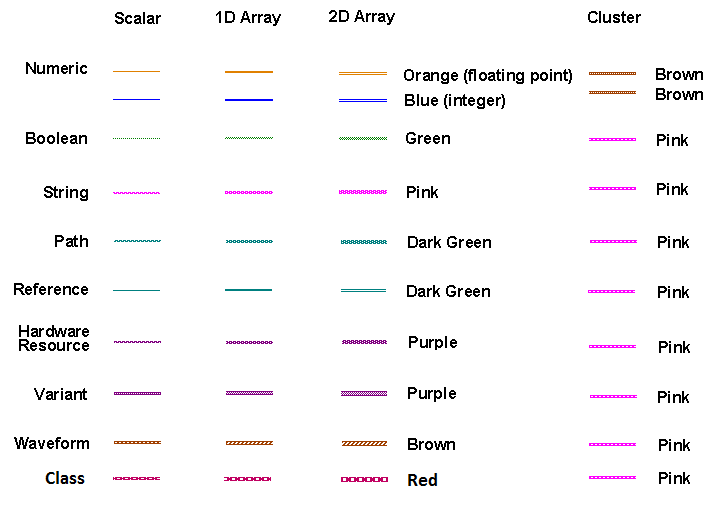
\includegraphics[width=0.8\textwidth]{pictures/Wire_Colors.png}
%\caption{The population of FMO with sink}\label{fig:1} 
\end{figure}

\begin{figure}[htbp]
\centering
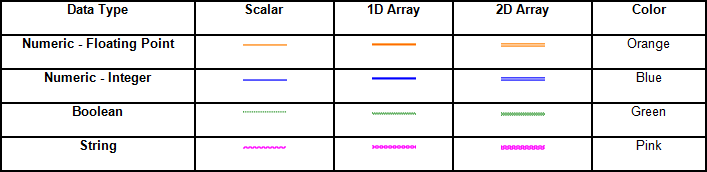
\includegraphics[width=0.8\textwidth]{pictures/wire_types.png}
%\caption{The population of FMO with sink}\label{fig:1} 
\end{figure}

\subsection{属性节点}
\subsection{事件}

\subsection{子Vi}
\begin{itemize}
\item 连线状态可以查看子Vi端口名称。
\end{itemize}



\section{用户界面设计}
界面好坏的最基本指标:
\begin{itemize}
\item 是否完成了交互功能
\item 是否可以简单直观地输入或获取信息
\item 界面的美观度
\end{itemize}

使用 Labview 开发一个项目的步骤:
\begin{itemize}
\item 收集需求; 
\item 设计;
\item 编码;
\item 测试;
\item 发布及维护
\end{itemize}

建议:先做用户界面设计,在做程序设计

理由:先设计程序结构,再设计界面,难免会朝着最可能简化编码工作方向去做。但是这样的界面往往不是最方便用户使用的界面。

另一方面,使用比较老的文本语言编程,设计用户界面时通常在草稿纸上画出原型。LabVIEW有独特的优势,可视化编程做的非常方便。有大量现成的控件,控件属性更改非常方便。因此,用户可以通过拖拽的方式,直接用LabVIEW来设计界面原型。

好的用户界面共有的特点:
\begin{itemize}
\item 一致性
\item 使用恰当的数据类型和控件类型;
\item 控件的分类排布合理、简洁
\end{itemize}

一致性:
让用户迅速接受并且方便的操作一个程序界面,最关键的一点就是让这个界面保存高度的一致性。

一致性包含以下多个方面的一致:
\begin{itemize}
\item 程序内部的一致性;\\
由于应用领域、面向的客户群体的不同,不同的软件可以有自己独特的风格。不论一个程序采用哪种风格,它内部不同界面,同一面板上的不同控件等,它们的风格应当保持一致。一个软件采用统一的风格,才会让用户有一种协调的感觉。
\item 与约定俗成的习惯保持一致;\\
很多设计或操作方法,已经被大家广为接受。它们也许不见得美观或优化,但是一旦习惯养成了,就很难被改变了。
\item 与真实事物保持一致;\\
有很多程序是对现实世界的模拟或模仿,这样的程序若希望便于被用户接受,最好是尽量与现实世界保持一致。LabVIEW编写的程序大多是测量、控制等有关,在这些领域,原本也存在着一些相关的仪器或设备。因此软件的界面可以借鉴这些仪器的外观。
\item 建立并遵循界面规范。\\
使界面保持一致性的最好办法就是在设计开发时遵循一定的规范。这个规范可以由公司内部定义,也可以遵循现有的行业规范。对于开发Windows系统风格的程序,可以遵循微软定义的界面规范。对于一般的LabVIEW程序,可以遵循LabVIEW程序开发规范。
\end{itemize}

界面元素的关联:

当一个界面上的元素比较多,找到自己想要的信息就要花上一小点时间。用户常常是一眼就看到了一个与自己想要的信息有一点关联的某个元素,他这时候会期望这个元素就有一定的提示信息,帮他加速找到自己想要的东西。因此,我们要在界面上,告诉用户哪些元素是相关的,或不相关的。

有很多手段可以把界面的元素之间的关联现实给用户,比如通过元素的排布、边框、空白、颜色、字体等等方式。我们总是在相关内容的附近去找想要的信息,所以逻辑上相关的控件或项目,应当在屏幕空间上相对临近。
单纯的把条目排在一起还是不利于用户查看。可以把它们按功能分成几个不同的区域,比如保存文件与 Project的操作在功能上相对独立一些,就可以用分隔线,帮它们的项目划分开。对于面板上的控件,功能相关的几个控件可以通过被边框围住、使用分割线、采用不同的间隙等等方法,让用户直观的感觉到他们在功能上的紧密关联。

帮助和反馈信息:

用户界面要照顾到那些不熟悉它的用户。为了方便用户了解界面的使用方法,需要给用户提供足够的帮助信息。对于 LabVIEW, 给用户提供提示主要通过以下几个手段:用户手册、在线帮助窗口、提示条、利用控件的标题、选项文字、直接把帮助文字写在界面上。不论何时,都应该尽量使用有意义的控件名称。

用户界面设计的限制:

目的:保障程序的可靠性

手段:限制用户的输入数据和操作
\begin{itemize}
\item 限制数据的输入;
\item 防止用户的误操作。
\end{itemize}



\section{调用DLL动态链接库}
参考:阮奇桢 《我和LabVIEW——一个NI工程师的十年编程经验》,北京航空航天大学出版社。感觉他写的这部分内容前后背景交代的很清楚,看起来舒服。

常用的计算机语言各有其特色,也有其不足。LabVIEW虽然功能强大,但编程时也时常会发现它缺少某些所需的功能,而这些功能也许恰恰已经有其他编程语言的DLL、ActiveX组件等提供。在这种情况下,最高效的方法莫不如让LabVIEW调用这些模块,直接利用其他语言或者操作系统已经实现的功能。


\subsection{DLL}
Dynamcis Linkable Library, DLL,动态链接库。从字母上理解,它是一种“程序库”。库内存放的是可供应用程序使用的函数、变量等。

“动态”是与“静态”相对应而来的。这里的动态和静态是指链接库中代码与使用它们的应用程序之间的链接方式。如果采用静态链接库,在生成应用程序时,库中的函数等都会被直接放入最终生成的可执行文件中;而使用动态链接库时,库中的函数等不会放到可执行文件中去,而是仍然保留在DLL文件内。当程序被运行时,再链接到动态链接库中的函数和变量等内容。

静态库的局限性比较大,C 语言编写的静态库只能在C 语言中使用,LabVIEW无法调用。而动态链接库则可以在多种编程语言中通用,即使用某一种语言编写出来的DLL可以在另一种语言编写的程序中使用。例如,使用C语言编写的DLL可以在LabVIEW中使用,反之亦可。

动态链接库的加载方式又分“动态”与“静态”两种。这里的动态和静态是指应用程序运行时,动态链接库代码被载入内存的方式。常用的方式是静态加载,指动态链接库在应用程序启动时随应用程序一起被载入内存。而动态加载方式是指,应用程序启动时并不载入动态链接库,只有在使用到动态链接库中某个函数时,才把动态链接库载入内存。

DLL最大的优势在于代表共享,只要某一功能以 DLL的形式提供出来了,其他的应用程序就可以直接使用这一功能,而不必再实现一份相同的代码了。DLL的使用非常普遍,比如 Windows 操作系统提供给应用程序调用的功能,就是以 DLL 的形式公布出来的。LabVIEW中若需使用某个系统功能,如读/写注册表等,即可通过调用 Windows 提供的 DLL 函数来完成。Windows 提供的这些完成系统功能的函数也被称为 Windows API(Application Programming Interface)。在常用的几个系统 DLL 中, kernel32.dll 提供了内存管理和进程调度相关的函数,user32.dll 中的函数则主要用于控制用户界面,gdi32.dll中的函数则负责图形方法的操作。在32位操作系统中,这些 Windows API 的 DLL 都被保存在 system32 目录下。
%
很多硬件设备的驱动程序也往往是以DLL方式提供的。此外,在互联网上还可以找到各种各样的 DLL。如果需要解析某种文件、使用某些常用的算法等,都可以先去互联网上搜索一下,是否有相关的DLL 库可供直接使用。

在LabVIEW中,经常会遇到需要使用DLL的情况,比如在程序中使用到某个以DLL方式提供的第三方驱动程序或算法;再比如,在一个大项目的开发中,出于效率和开发人员喜好等因素的考虑,可能使用C++语言实现软件的运算部分,并把这些功能构建在DLL文件中,再使用 LabVIEW 编写程序的界面部分,并通过调用编写好的 DLL 来调用运算部分的功能。


\subsection{CLN和CIN节点}
在LabVIEW中,通过“互连接口$\rightarrow$库与可执行程序$\rightarrow$调用库函数” 节点来调用 DLL 中的函数。调用库函数节点常简称为 CLN 节点,是英文 Call Library Function Node 的缩写。在同一函数选板上,它旁边的一个节点是“代码接口”(Code Interface Node),简称 CIN节点。
在CLN节点出现以前,LabVIEW只能通过CIN节点调用C 语言编写的函数。现在有了CLN,可以不再考虑使用CIN了。
CIN节点不能调用动态链接库中的函数,只能调用按照特定方式编译出来的程序代码。稍有差错,程序就无法正常运行。CIN所调用的程序模块不通用,而且限制颇多,CLN节点出现之后,就很少有人再使用CIN节点了。


\subsection{LabVIEW调用DLL中的函数以及手动配置CLN节点}
这部分在参考书中写的非常详细。这里简单说下。一个CLN节点被拖到程序框图上后,需要进行对其配置才能使用。双击CLN节点,则弹出其配置对话框,该对话框有4个选项卡,如下图所示
\begin{figure}[htbp]
\centering
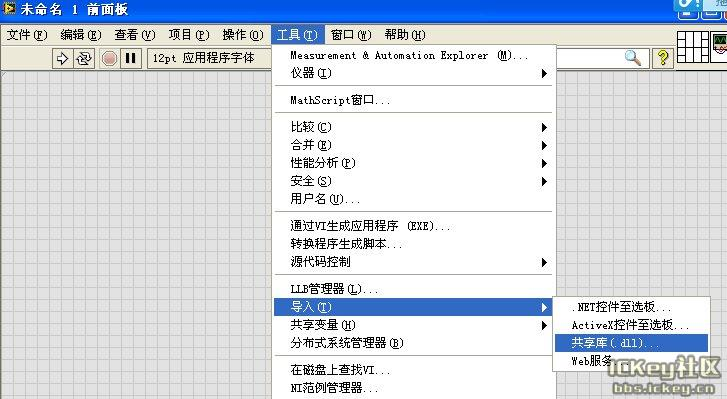
\includegraphics[width=0.9\textwidth]{pictures/1.png}
%\caption{The population of FMO with sink}\label{fig:1} 
\end{figure}
\begin{itemize}
\item 第一个选项卡是被调用函数的信息,主要有
\begin{itemize}
\item “库名或路径”列表框。用于填写DLL文件名和DLL的全路径。 在系统路径下的DLL,直接输入文件名即可,否则需要全路径。
\item “在程序框图中指定路径”选项。若没有勾选,则是LabVIEW静态调用了这个DLL;若勾选,则是动态调用。具体说明参见参考书。
\item “函数名”列表框。用于输入需要调用的DLL中的函数。如果选用静态加载方式,并已输入了正确的DLL文件全路径,这里会列出DLL中所有允许被外部调用的函数,用户只要在下拉列表框中选取一个即可。
\item “线程”选项。用于选择被调用的DLL函数在何线程内运行。 CLN节点的线程选项只有两项:“在UI线程中运行”和“在任一线程中运行”。在程序框图上直接就可以看出一个CLN节点选用的是什么线程。如果是“在UI线程中运行”,则节点颜色是比较深的桔黄色;如果是“在任一线程中运行”,则节点是比较淡的黄色。详细说明见参考书。
\item “调用规范”。用于指明被调用函数的参数压栈规范。Windows API一般使用 stdcall,标准C的库函数大多使用C call。
\end{itemize}
\item 第二个选项卡是配置参数选项卡。使用CLN节点,最困难部分就是把函数参数的数据类型映射为相应的LaVIEW中的数据类型。这也是最关键的。
\item 第三个选项卡是设置回掉函数选项卡。可以使用这些回调函数在特定的情形下完成初始化、清理资源等工作。如果为 Reserve 选择了一个回调函数,那么当一个新的线程开始调用这个 DLL 时,这个回调函数首先被调用。可以利用这个函数为新线程使用到的数据做初始化工作。如果一个线程使用了这个 DLL,在线程结束时,它会去调用 Unreserve 中指定的回调函数。Abort 中指定的函数用在 VI 非正常结束时被调用。比如按 Abort 按钮让一个 VI 停止,而不是让它运行完。这里的几个回调函数必须要由 DLL 的开发者按照特定的格式实现。它的原型就是 Prototype for these procedures 中列出的那个。如果你使用的 DLL 不是专为 LabVIEW 设计的,一般不会包含这样的回调函数。
\item 第四个是错误处理方式选项卡。这上面说明写得已经很详细了。
\end{itemize}


%\subsubsection{数据类型参数的设置}



\subsection{把DLL中的函数包装成子VI}
在LabVIEW中调用DLL的函数,最大的困难在于把函数参数的数据类型映射为相应的LabVIEW中的数据类型。在手工设置CLN节点前,可以优先考虑使用导入共享库工具,以自动生成配置CLN节点。这个工具在“工具$\rightarrow$导入$\rightarrow$共享库”菜单项中,专门用于把DLL中的函数包装成VI,生成的每个VI中最主要的部分就是一个CLN节点;它能够自动设置函数的参数。有了这个工具,用户就不再需要费脑筋去考虑数据类型匹配的问题了。

这个工具可能无法直接处理一些非常特殊的数据类型(如字符串数组)和函数(如回调函数),但在大多数情况下,都能够把DLL中的函数包装成可以正确运行的VI。如果有现成的DLL打算在LabVIEW中使用,首先应该考虑用这个工具,把DLL中所有的函数都包装成VI,再使用起来,就方便多了。

如果DLL是C++编写的,并且使用了C++的类作为接口,这样的DLL是没办法在LabVIEW中直接调用的。CLN节点只能调用符合标准C语言函数接口的DLL。若项目中必须使用某个C++ DLL,则可以在其上再用C语言写一个C接口DLL,作为它和LabVIEW之间的中间层。LabVIEW调用这个中间层DLL提供的函数,中间层函数再调用C++接口的DLL函数。



\subsubsection{应用举例}
Labview是一个图形化软件库,不但支持NI官网硬件,还支持众多第三方硬件,这些硬件提供的驱动基本上是DLL的方式,需要在labview里面调用。其实,labview也可以支持自制MCU硬件。只要能提供相应的DLL就行,甚至,如果能在labview和IDE开发环境之间建立接口,一个labview子VI,就可以实现在labview运行状态下,配合MCU仿真器,实现  图形化程序到MCU的下载,脱离了C代码的编写,开发更加快速很方便!

     今天为大家分享一个深度调用DLL的方法,为什么是深度调用DLL。因为,调用的不是DLL本身。而是由DLL生成的子VI函数。下面重点分享如何将DLL生成可以被labveiw调用的子VI。


一、要会编写DLL

     动态链接库英文为DLL,是Dynamic Link Library 的缩写形式,DLL是一个包含可由多个程序同时使用的代码和数据的库。编写DLL文件需要有VC++功底。比如平时经常开发MCU软件,积累了很多C驱动代码,如果能够按照规范,就可以生称DLL文件。
     
     二、要有相应的DLL.H文件
     
     编写了DLL文件外,还要有H文件才行。通常开发数据采集卡的厂家只会提供DLL文件本身,而不会提供编写DLL文件用的C代码和H文件。所以,那些数据采集卡只能采用直接调用DLL的方式。而自制硬件中,C代码和H文件是自己编写,所以,可以很容易实现DLL转labview的子VI。


三、应用实例讲解:

     因为一个MCU内容太多,短时间内实现也不现实。就采用一个开源厂家的例子来实现。
CH375是国内厂家江苏沁恒(\url{www.wch.cn})生产的一个USB芯片,支持HOST主机方式和SLAVE设备方式。速度可以实现全速方式,在一些总线设备和USB数据采集设备上采用很多。厂家开源了一CH375DLL.DLL和一个CH375DLL.H文件。下面分享一下过程:


\newpage
1、打开labview界面,建立一个空VI。在【工具】选项中,选择导入—共享库(dll),如图:
\begin{figure}[htbp]
\centering
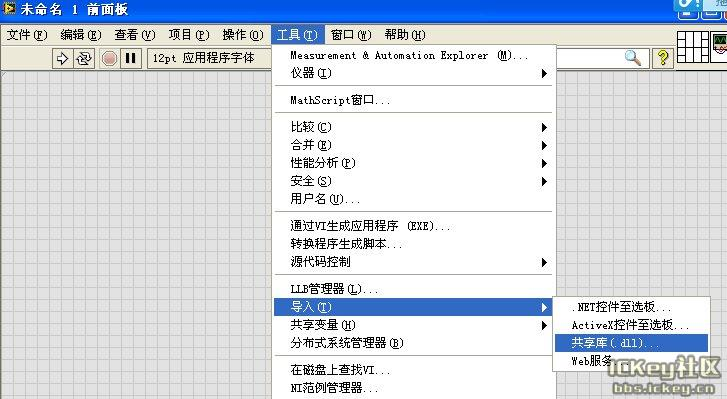
\includegraphics[width=0.9\textwidth]{pictures/1.jpg}
%\caption{The population of FMO with sink}\label{fig:1} 
\end{figure}

2、在出现的界面中,为共享库创建新Vi,进入下一步:
\begin{figure}[h!]
\centering
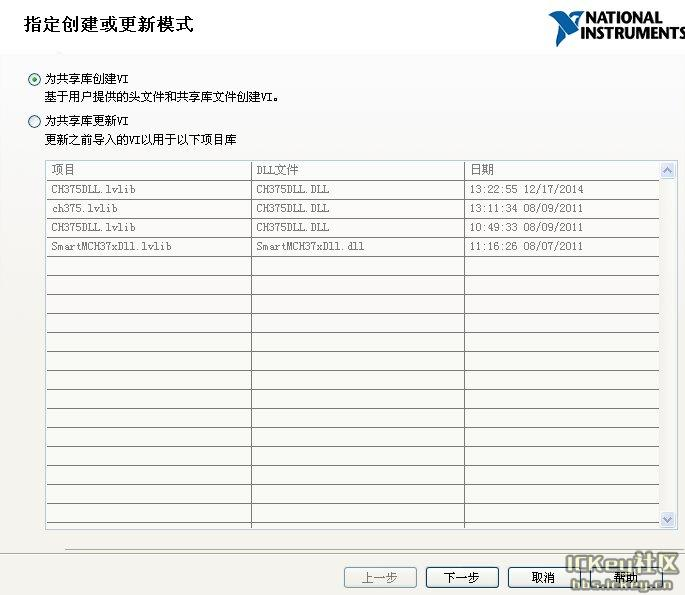
\includegraphics[width=0.9\textwidth]{pictures/2.jpg}
%\caption{The population of FMO with sink}\label{fig:1} 
\end{figure}

\newpage
3、选择共享库及头文件,这里把CH375DLL.DLL和CH375DLL.H文件载入:
\begin{figure}[h!]
\centering
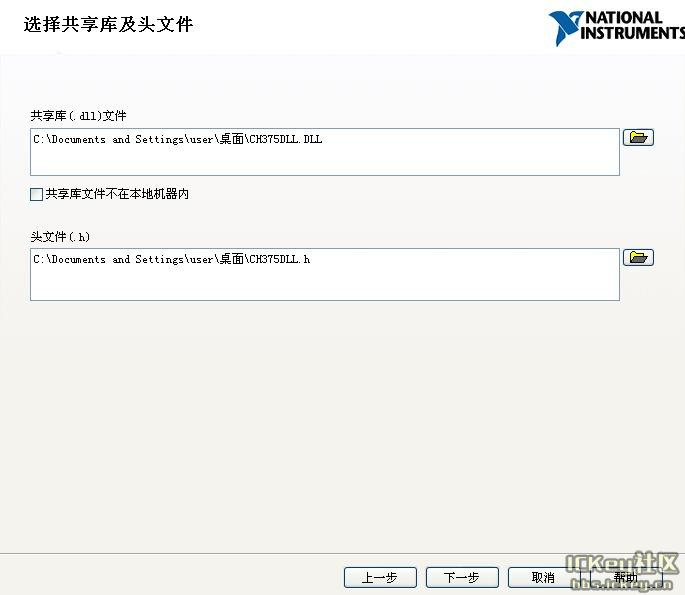
\includegraphics[width=0.75\textwidth]{pictures/3.jpg}
%\caption{The population of FMO with sink}\label{fig:1} 
\end{figure}

4、配置包路径和宏定义命令,这里空着不填,进入下一步:
\begin{figure}[h!]
\centering
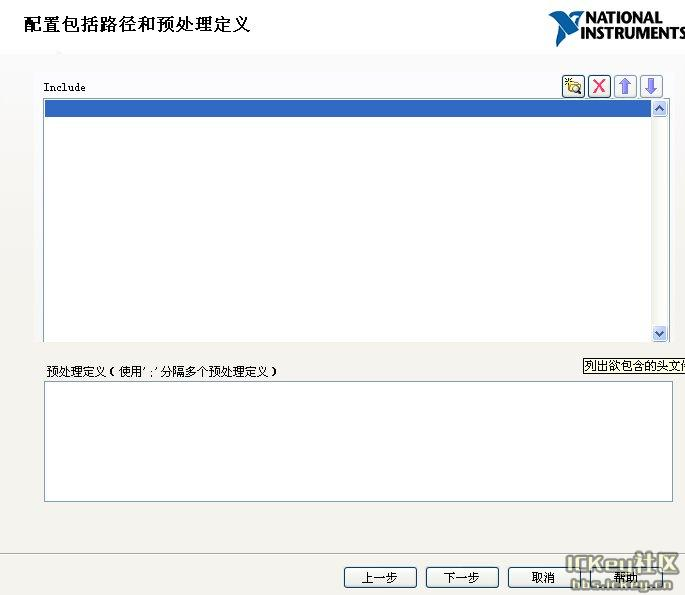
\includegraphics[width=0.75\textwidth]{pictures/4.jpg}
%\caption{The population of FMO with sink}\label{fig:1} 
\end{figure}

5、全部勾选DLL库里面的函数定义文件,下一步:
\begin{figure}[h!]
\centering
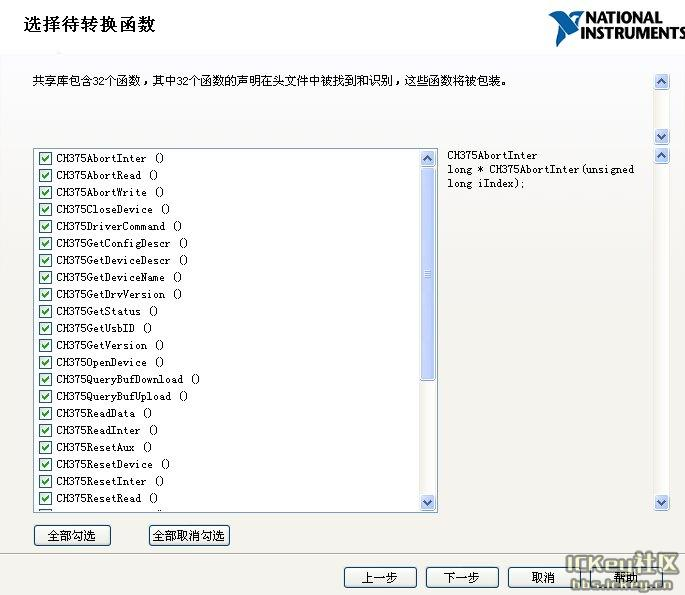
\includegraphics[width=0.75\textwidth]{pictures/5.jpg}
%\caption{The population of FMO with sink}\label{fig:1} 
\end{figure}

 6、配置好生成的VI库的路径和名称:
\begin{figure}[h!]
\centering
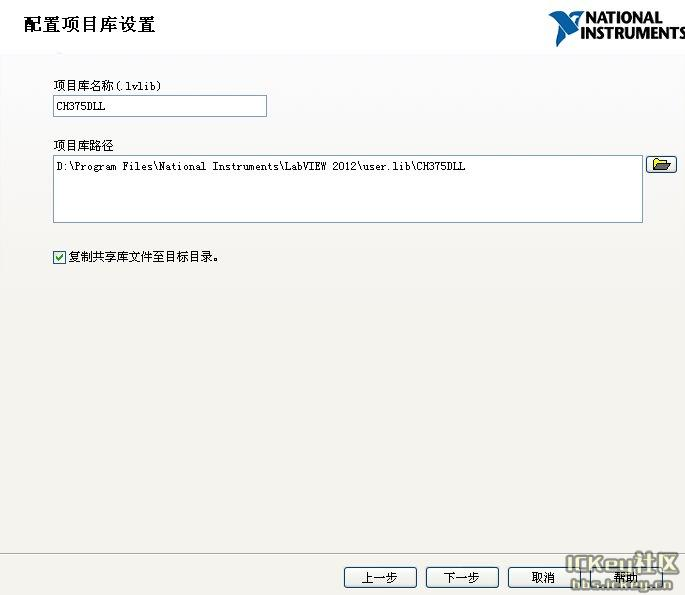
\includegraphics[width=0.75\textwidth]{pictures/6.jpg}
%\caption{The population of FMO with sink}\label{fig:1} 
\end{figure}

7、选择错误处理方式,这里有多种方式,可以选择简易错误处理:
\begin{figure}[h!]
\centering
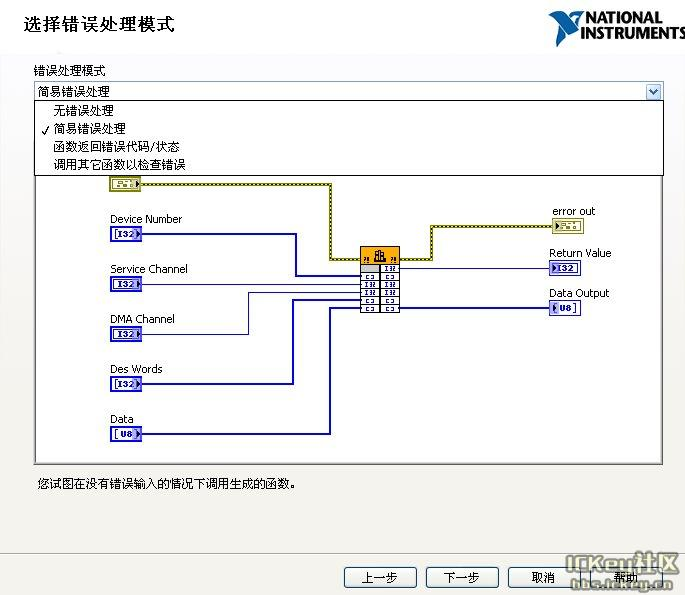
\includegraphics[width=0.75\textwidth]{pictures/7.jpg}
%\caption{The population of FMO with sink}\label{fig:1} 
\end{figure}

8、配置VI和控件,这里和DLL一样设置如图:
\begin{figure}[h!]
\centering
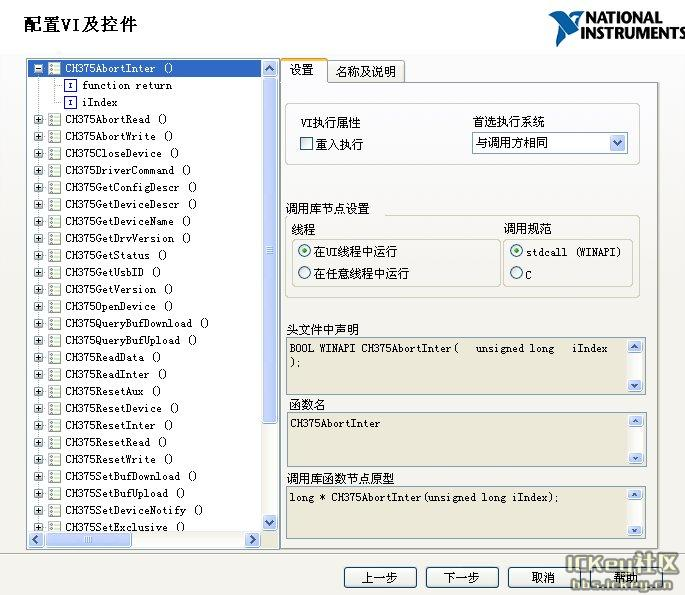
\includegraphics[width=0.75\textwidth]{pictures/8.jpg}
%\caption{The population of FMO with sink}\label{fig:1} 
\end{figure}

9、最后,是一个生成总结:
\begin{figure}[h!]
\centering
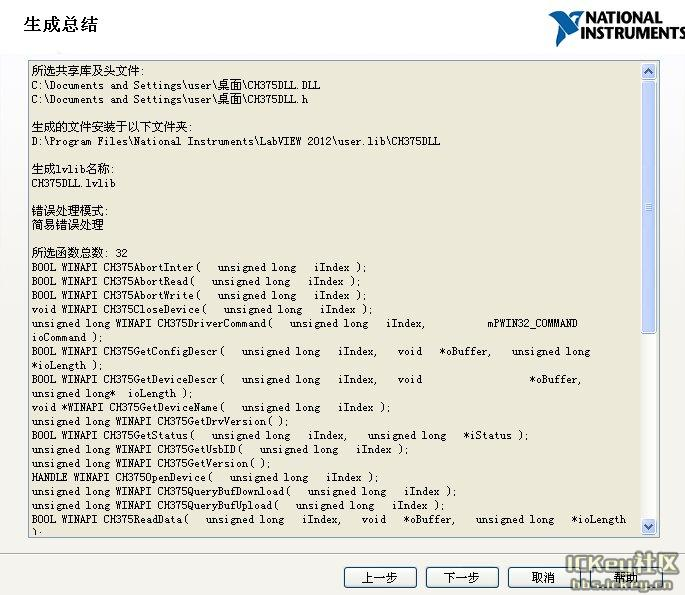
\includegraphics[width=0.75\textwidth]{pictures/9.jpg}
%\caption{The population of FMO with sink}\label{fig:1} 
\end{figure}

10、然后,点下一步就可以了:
\begin{figure}[h!]
\centering
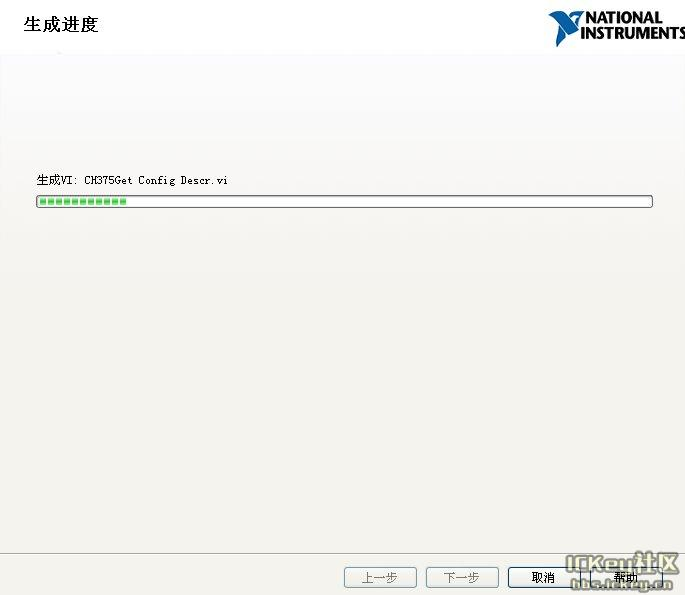
\includegraphics[width=0.75\textwidth]{pictures/10.jpg}
%\caption{The population of FMO with sink}\label{fig:1} 
\end{figure}

\begin{figure}[h!]
\centering
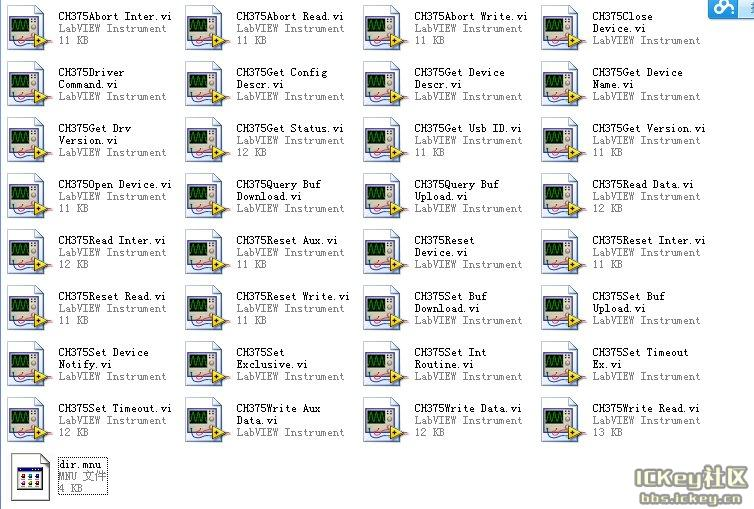
\includegraphics[width=0.75\textwidth]{pictures/11.jpg}
%\caption{The population of FMO with sink}\label{fig:1} 
\end{figure}


11、从这里调入vi,看到没,调用后,直接进行连线就可以了,不像原来那样看着眼花缭乱了。
\begin{figure}[h!]
\centering
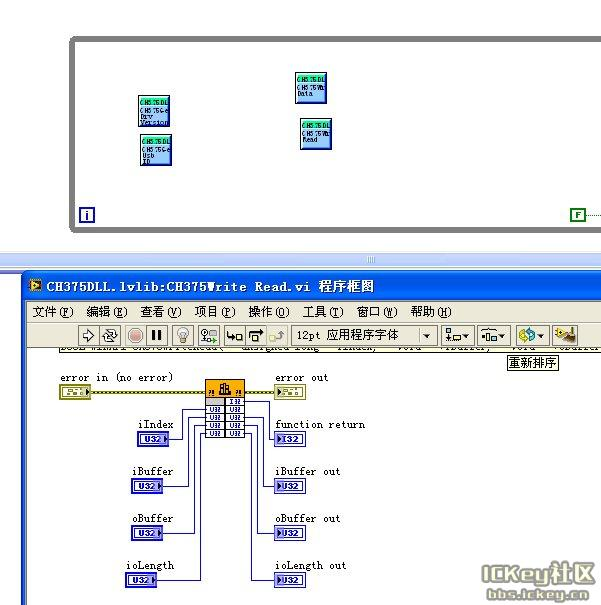
\includegraphics[width=0.75\textwidth]{pictures/13.jpg}
%\caption{The population of FMO with sink}\label{fig:1} 
\end{figure}


\subsubsection{调用DLL时遇见的问题}
在使用DLL时,最大的困难就是把函数参数的数据类型映射为相应的LabVIEW中的数据类型。LaBVIEW提示:

{\color{blue}\emph{未定义符号可能会造成函数和参数无法被识别。如要解决该问题,检查头文件并确定是否必须添加预定义符号。单击上一步按钮返回至向导的前一页并添加预定义符号(例如,“NIAPI\_stdcall \_stdcall” 或 ``NIAPIDEfined = 1'')} }

归咎原因就是头文件中哦你搞得一些类型定义不符合标准C语法,而使解析器无法获得正确的定义。DLL函数的头文件中可能使用了某个系统定义的数据类型,数据类型的定义在 windows.h中(windows.h是Windows SDK 的一个文件,VC等开发环境中常常带有 Windows SDK),要正确解析必须得到这些数据类型,也就是找到 windows.h 这个头文件,用户须把windows.h文件的全路径加在“包括路径”中。例如 Visual C++ 6.0编译环境中头文件位于安装目录下 VC98文件夹下的 Include文件中。

而“预处理定义”中,当用户需要写一些宏定义,那么就写在这个位置,如
添加如下代码:

ULONG = unsigned long; VOID = void; LONG = long; UCHAR = unsigned char; PUCHAR = unsigned char*;
PULONG = unsigned long*; WINAPI; BOOL=bool; USHORT = unsigned short; PUSHORT = unsigned short*;

这样就不会出现问题了。


\section{NI-DAQmx 数据采集}
参考书:
\begin{itemize}
\item 《LabVIEW 大学实用教程 (第三版)》 Jeffrey Travis, Jim Kring 著,乔瑞萍 等译。LabVIEW for Everyone (Graphical Programming Made Easy and Fun, Third Edition ) 第二章、第十章和第十一章。
请详细阅读相关章节。这里只记录比较重要的部分。

\item 《LabVIEW 实践教程》 Robert H. Bishop,National Instruments著,乔瑞萍 林欣 等译
\end{itemize}



\subsection{NI-DAQmx简介与安装}
(1)简介

 DAQ,Data AcQuisition,是一个术语,即数据采集,是实现测量现实世界信号如电压,并把这些信息发送到计算机用于处理、分析、储存或其他数据操作的过程。而NI-DAQmx 则是NI公司的跨平台DAQ设备驱动程序,包含了所有NI公司DAQ设备的驱动。NI-DAQmx代替了传统的NI-DAQ(以前称为“NI-DAQ”),并且在传统的NI-DAQ基础上提供了诸多改进,如:改进了状态模型、多线程驱动程序、意外情况下的健壮性、简化的同步、降低了LabVIEW框图的混乱、从简单到高级程序的平滑过渡。NI-DAQmx优于先前NI-DAQ的显著特定就是包含了DAQ Assistant以配置通道和完成测量任务。

信号的采集需要对信号有所了解,比如信号类型、一个信号的五种测量角度常见的转换器和信号调节等,这里不详细讲述,参考书中相关章节有叙述。这里需要注意的是,Nyquist-Shannnon采样定理,采样频率必须大于被采集信号最高频率的两倍。但是为了充分保持信号的形状,采样频率通常至少为信号最高频率的5$\sim$10倍。


(2)安装

NI-DAQmx是与LabVIEW单独安装的,它们版本之间的兼容性如下图所示,可以在官网查询。安装过程比较简单,跟通常软件安装过程一样,需要注意的是安装过程比较长。
\begin{figure}[h!]
\centering
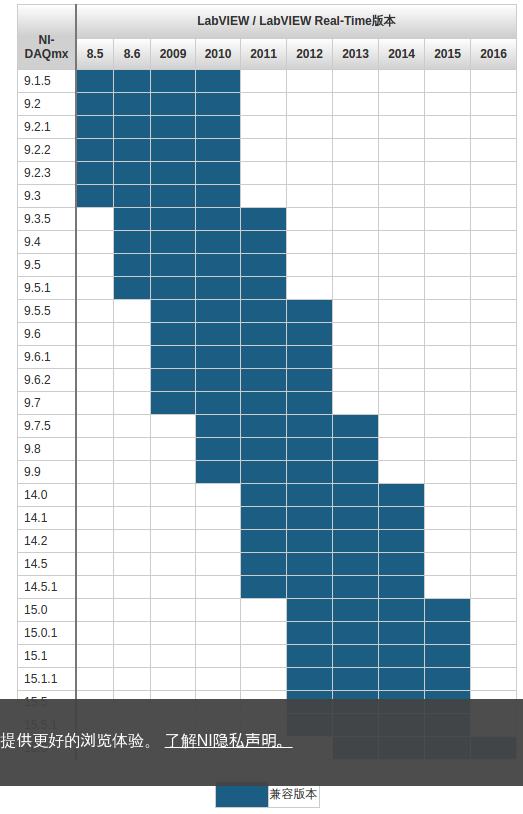
\includegraphics[width=0.5\textwidth]{pictures/ni-daqmx.png}
\caption{NI-DAQmx与LabVIEW的版本兼容性}
\end{figure}


\subsection{MAX及创建NI-DAQmx虚拟设备}
MAX,Measurement \& Automation Explorer,是在NI-DAQmx和LabVIEW之间的实用软件,目前只支持 Windows平台。它是一个Windows的软件接口,用于配置和测试硬件,可以访问NI公司的所有设备(包括DAQ,GPIB,VXI等)。换句话说,就是一个用于建立各种卡及通道配置参数的配置工具。 Windows设备管理器管理着用户系统中的所有硬件,其中包括NI公司的DAQ设备。MAX会读取设备管理器在Windows注册表中记录的信息,并为用户系统中的每个NI DAQ卡分配逻辑设备号。用户可以通过该设备号访问LabVIEW中的卡。

用户可以通过访问计算机中哦你搞得设备管理器找到数据采集设备,如 Data Acquisition Devices 中列出了安装在计算机上的所有DAQ卡。选取一个DAQ卡,选择Properties或双击该DAQ卡,可以看到一个多页面的对话框。 General 显示了与卡相关的整体信息。可以通过Resources指定该卡占用的系统资源,比如中断级、DMA以及软件可配置卡的基址。Driver指明了该DAQ卡驱动程序的版本及位置。

用户可以在NI-DAQmx7.5及新版本中利用MAX创建NI-DAQmx虚拟设备,这样用户可以建立原型系统,在进行实际数据采集前,测试数据采集应用程序。当需要实际采集时,还可以使用MAX可移植配置向导,将NI-DAQmx虚拟设备的配置输入导入到物理设备中。
创建NI-DAQmx虚拟步骤如下:
\begin{enumerate}
\item 打开MAX(Measurement \& Automation),可以点击桌面图标打开,也可以从LabVIEW打开。

\item 右击“设备和接口(Devices and Interfaces)”弹出快捷菜单并选择“新建(Create New)”。

\item 一个对话框会提示用户选择要添加的设备。选择 “仿真NI-DAQmx设备或模块化仪器(NI-DAQmx Simulated Device)” 并点击 “完成(Finish)”。

\item 在“选择设备(Choose Device)”对话框中选择需要的虚拟设备,比如 M series DAQ。

\item 选择 NI PCI-6251 并单击 OK 按钮。
\end{enumerate}


\subsection{DAQ助手}
DAQ Assistant,DAQ助手,是一个用来配置测量任务及通道的图形界面接口。DAQ助手位于 Functions>Measurement I/O>DAQmx-Data Acquisition 选项板中。将DAQ助手拖入框图中就可以将其弹出。当DAQ 助手 置入框图中时,DAQ助手对话框将会自动出现。一旦打开DAQ 助手,配置NI-DAQmx任务所需步骤与使用MAX配置NI-DAQmx任务的步骤基本一致。使用DAQ助手构建数据采集VI的通用过程如下:
\begin{itemize}
\item 打开一个新的VI。
\item 在框图中拖入DAQ 助手。
\item 出现 DAQ助手对话框帮助用户配置测量任务。
\item 配置、命名及测试NI-DAQmx任务。
\item 单击OK按钮以返回框图。
\item 编辑前面板和框图完成VI。
\end{itemize}

如果使用DAQ助手配置了DAQmx任务,则该任务就是一个本地任务,因此,它不能保存到MAX中被其他应用使用。如果想要使任务对于其他应用也可用,可是通过DAQ 助手生成NI-DAQmx Task Name控件使其保存到MAX中并在其他应用中使用。DAQmx Task Name Constant 是为了与DAQ卡进行通信而在DAQ VI中使用的一种LabVIEW数据类型。

\begin{itemize}
\item 通过右击框图中的DAQ 助手 弹出快捷菜单并在下拉菜单中选择 Convert to NI-DAQmx Task;
\item 此时会出现DAQ 助手以便重新配置任务;
\item 退出DAQ助手后,则完成转换,该DAQmx任务就存在于MAX中并且可以被其他应用使用。
\end{itemize}

如果想要在应用中使用来自MAX的DAQmx任务,则按如下步骤:
\begin{itemize}
\item 首先在 Functions>Measurement I/O>NI DAQmx-data Acquisition选项板中找到DAQmx Task Name Constant ,并拖入框图中。
\item 任务名称可以通过鼠标手形工具单击 DAQmx Task Name Constant浏览选择。
\end{itemize}



\subsection{NI-DAQmx VI}
如果说DAQ助手是数据采集的图形化配置界面,那么NI-DAQmx VI则是DAQ助手配置的底层VI。
在涉及与其他操作联动时,采用NI-DAQmx VI的形式更为可靠。
NI-DAQmx VI 是一种被称为多态VI的特殊VI,其结果是能够适应不同DAQ功能的一组核心VI,比如模拟输入、模拟输出、数字I/O等等。在LabVIEW后面板上,右键打开函数(Functions)选项板,单击“测量I/O(Measure I/O)>DAQmx 数据采集(Measurement I/O>DAQmx-data Acquisition)”访问该选项板。

Windows版的LabVIEW DAQ VI使用的是 Windows 版 32位动态链接库(DLL)形式的 NI公司标准NI-DAQ。LabVIEW安装程序将NI-DAQ DLL 安装在 Windows$\backslash$System32目录下。nidaq32.dll文件是用户使用的DAQ卡的高级接口,安装在Windows$\backslash$System32目录下。随后,nidaq32.dll文件将与Windows注册表对接以获取由MAX定义的配置参数。

NI-DAQmx VI使用非常简单,主要有如下几个步骤:
\begin{itemize}
\item 创建一个任务(或引用一个MAX DAQmx任务)。
\item 启动任务。
\item 读或写,以及根据需要重复。
\item 停止任务。
\item 清除任务。
\end{itemize}
需要注意的是:
\begin{itemize}
\item 用户不一定必须启动任务,通常读或写操作会自动启动任务。
\item 在清除任务之前不必停止任务。如果任务正在运行,清楚操作将先停止任务。
\end{itemize}




\section{EMCCD}
\subsection{CDD类型简介}
CCD, Charge-Coupled Device,电荷耦合器。\footnote{\url{https://en.wikipedia.org/wiki/Charge-coupled_device}}
简单来说,在一个用于感光的CCD中,有一个光敏区域(硅的外延层),和一个由移位寄存器制成的传感区域(狭义上的CCD)。
图像通过透镜投影在一列电容上(光敏区域),导致每一个电容都积累一定的电荷,而电荷的数量则正比于该处的入射光强。用于线扫描相机的一维电容阵列,每次可以扫描一单层的电容;而用于摄像机和一般相机的二维电容阵列,则可以扫描投射在焦平面上的图像。一旦电容阵列曝光,一个控制回路将会使每个电容把自己的电荷传给相邻的下一个电容(传感区域)。而阵列中最后一个电容里的电荷,则将传给一个电荷放大器,并被转化为电压信号。通过重复这个过程,控制回路可以把整个阵列中的电荷转化为一系列的电压信号。在数字电路中,会将这些信号采样、数字化,通常会存储起来;而在模拟电路中,会将它们处理成一个连续的模拟信号(例如把电荷放大器的输出信号输给一个低通滤波器)。

\textbf{Frame transfer CCD,帧转移CCD。}A frame transfer CCD is a specialized CCD, often used in astronomy and some professional video cameras, designed for high exposure efficiency and correctness.

The normal functioning of a CCD, astronomical or otherwise, can be divided into two phases: exposure and readout. During the first phase, the CCD passively collects incoming photons, storing electrons in its cells. After the exposure time is passed, the cells are read out one line at a time. During the readout phase, cells are shifted down the entire area of the CCD. While they are shifted, they continue to collect light. Thus, if the shifting is not fast enough, errors can result from light that falls on a cell holding charge during the transfer. These errors are referred to as "vertical smear" and cause a strong light source to create a vertical line above and below its exact location. In addition, the CCD cannot be used to collect light while it is being read out. Unfortunately, a faster shifting requires a faster readout, and a faster readout can introduce errors in the cell charge measurement, leading to a higher noise level.

A frame transfer CCD solves both problems: it has a shielded, not light sensitive, area containing as many cells as the area exposed to light. Typically, this area is covered by a reflective material such as aluminium. When the exposure time is up, the cells are transferred very rapidly to the hidden area. Here, safe from any incoming light, cells can be read out at any speed one deems necessary to correctly measure the cells' charge. At the same time, the exposed part of the CCD is collecting light again, so no delay occurs between successive exposures.

\textbf{ICCD, Intensified Charge-Coupled Device,增强电子耦合器。}

An intensified charge-coupled device (ICCD) is a CCD that is optically connected to an image intensifier that is mounted in front of the CCD.

An image intensifier includes three functional elements: a photocathode, a micro-channel plate (MCP) and a phosphor screen. These three elements are mounted one close behind the other in the mentioned sequence. The photons which are coming from the light source fall onto the photocathode, thereby generating photoelectrons. The photoelectrons are accelerated towards the MCP by an electrical control voltage, applied between photocathode and MCP. The electrons are multiplied inside of the MCP and thereafter accelerated towards the phosphor screen. The phosphor screen finally converts the multiplied electrons back to photons which are guided to the CCD by a fiber optic or a lens.

An image intensifier inherently includes a shutter functionality: If the control voltage between the photocathode and the MCP is reversed, the emitted photoelectrons are not accelerated towards the MCP but return to the photocathode. Thus, no electrons are multiplied and emitted by the MCP, no electrons are going to the phosphor screen and no light is emitted from the image intensifier. In this case no light falls onto the CCD, which means that the shutter is closed. The process of reversing the control voltage at the photocathode is called gating and therefore ICCDs are also called gateable CCD cameras.

Besides the extremely high sensitivity of ICCD cameras, which enable single photon detection, the gateability is one of the major advantages of the ICCD over the EMCCD cameras. The highest performing ICCD cameras enable shutter times as short as 200 picoseconds.

ICCD cameras are in general somewhat higher in price than EMCCD cameras because they need the expensive image intensifier. On the other hand, EMCCD cameras need a cooling system to cool the EMCCD chip down to temperatures around 170 K. This cooling system adds additional costs to the EMCCD camera and often yields heavy condensation problems in the application.

ICCDs are used in night vision devices and in various scientific applications.


\textbf{EMCCD,Electronic Multiplying Charge Coupled Device,电子倍增耦合器},是一种增强型帧转移CDD。但它的输出信号质量远高于普通CCD且优于其他增强型CCD,提供出色信噪比的CCD。\footnote{参考文献:[1]韩露,熊平. EMCCD工作原理及性能分析[J]. 传感器世界,2009,(05):24-28.}EMCCD是一块基于硅的半导体芯片,具有二维矩阵的光电传感器或像素。EMCCD技术,有时也被称作“片上增益”技术,是一种微弱光信号增强探测技术。而“片上增益”这一功用的实现就是在移位寄存器的后面加了增益寄存器。该寄存器可以使信号在噪声加入前就被倍增到一定的程度,使放大器的读出噪声并不能影响信号的质量,或者说减小对信号的影响。


\subsection{EMCCD和ICCD的异同}
参考:\url{www.lustervision.com/new-product/emccdxj20150528.shtml}

EMCCD也就是电子倍增CCD,它和ICCD被成为业内最为灵敏的两种CCD。现在罐子探测领域的高速发展对探测器灵敏成都的要求越发的苛刻,而EMCCD技术对于这种越来越苛刻的要求做出了完美的答复。所以EMCCD相机也应用领域中较为常见。那么EMCCD相机的优点有什么?我们可以通过比较ICCD和EMCCD来看。

ICCD的放大原理是让光先通过光电阴极激发出电子,电子再进入微通道版进行放大,放大后的电信号通过轰击荧光屏激发出荧光,最后再让荧光通过光纤耦湖综合透镜,最终让荧光合到普通CCD靶面上成像。ICCD拥有两个特点:一是想要实现纳秒量级别的快门控制时间,只需要在光电阴极上加脉冲电压,这样就可以做超快时间分辨探测;二是信号能力因为电子轰击增益而加强。缺点也是非常明显的,在使用时空间分辨率会有一定损失。

EMCCD技术就是在普通的CCD读出寄存器后面增加一个增益寄存器,从而将电子信号进行放大。其中的原理就是利用电子在转移过程中产生的“撞击离子化”效应,从而产生新的电子。暗电流通过制冷后可以起到抑制噪声的作用,这样信号增益提取就可以有效地进行了。EMCCD相对于ICCD的好处就是控件分辨率很好,成像很快,不过缺点就是时间分辨率不如ICCD。

EMCCD和ICCD的比较:
\begin{itemize}
\item EMCCD不会因为增强器中有几百上千伏的高压起到的高增益环境下,引入的强信号损毁增强器,ICCD技术就有可能发生这种情况。
\item EMCCD拥有毫秒级别的时间分辨;ICCD技术可以精确到纳秒级。
\item EMCCD采用的CCD芯片可以将背照式峰值量子效率提高到90\%;而ICCD通过的光电转换通过光电阴极实现,最多只能将峰值量子效率提高到50\%,甚至不足。
\item EMCCD的像增强器并没有被出口管制;而ICCD因为成本高、价格高,被限制出口。
\item EMCCD的空间分辨率只受像素大小影响,分辨率比ICCD高,适合生命科学领域。
总的来说,通过比较ICCD和EMCCD技术特点,EMCCD相机的有点还是比较多的,因此EMCCD技术也能针对应用领域内越来越高的要求,而给出一个个完美的答复。
\end{itemize}




\section{PI-MAX3型CCD LabVIEW参数设置学习}
快速测量的示例vi都在 \verb|ExamplesXX_ver\Fast Examples|目录下找到。需要注意的是安装后的目录下的vi文件或许有些缺失,最好直接到安装光盘Examples目录下寻找。示例vi都是以Ex开头的。
%
%我们的EMCCD初始化vi命名为:Spectro\_Init.vi,
外触发快速测量CCD参数初始化vi,
由ExOpenGlobalcam.vi、ExOpenGlobalPulser.vi、ExSetupROI.vi、ExSetupExtSuperSyncro.vi组成。
这些都是软件包提供的快速测量示例vi,需要注意的是这些示例vi中的子vi有重复,具体使用时需要做些删减。示例vi并不是最底层的vi,是可以查看后面板,供用户学习使用的。而底层vi,后面板有密码保护,无法查看,但有详细的说明文档。接下来对各示例vi进行详细说明。参数设置要注意结合EMCCD的用户手册、LightField软件用户手册(或WinSpec软件用户手册)一起研究。

(1) ExOpenGlobalcam.vi、 ExOpenGlobalPulser.vi:打开CCD,创建全局变量,是快速测量的关键。

快速测量是通过全局句柄(Global Handles)实现的。必须首先运行ExOpenGlobalcam.vi,再运行ExOpenGlobalPulser.vi,这样就完成了全局句柄的创建。在整个LabVIEW程序运行过程中,只要不关闭Camera,这两个子vi只需运行一次。这两个vi很简单,无需做任何修改,直接使用即可。

ExOpenGlobalcam.vi由多个底层vi构成。
\begin{itemize}
\item 第一个vi: CamHandle.vi。全局变量。
\item 第二个vi: InitToolkit.vi。SITK软件包初始化。
\item 第三个vi: CameraOpen.vi。设置Camera编号以及初始默认参数。
\item 第四个vi: ToolKitIsError.vi。检查软件包是否有误。
\end{itemize}

ExOpenGlobalPulser.vi由多个底层vi构成。
\begin{itemize}
\item 第一个vi: PulserHandle.vi。全局变量。
\item 第二个vi: PulserOpen.vi。
\item 第三个vi: ToolKitIsError.vi。检查软件包是否有误。
\end{itemize}


(2) ExSetupROI.vi: ROI, Region Of Interest。CCD曝光参数设置,由多个示例vi和底层子vi构成。
\begin{itemize}
\item 第一个子vi是底层vi: CameraSkips.vi。This Vi will allow the setting of the skip parameters in the camera. This will allow a number of pixels to be ``passed over" and  allows for a quicker read of the camera.
\\\textbf{参数:}Minimum Block Size:2; Number of Minimum blocks:5。
\\ \textbf{参数说明}:这部分参数取值比较复杂,建议使用厂家默认值。在WinSpec用户手册,Vertical Skips 部分有详细说。在LightField用户手册,Appendix D:Reference Topics>Cleaning and Skipping Algorithm部分有更详细的说明。
\begin{itemize}
\item Minimum Block Size: The number of lines to group on the CCD shift register before discarding (for lines that are to be skipped). Sets the size, in rows, of the skip blocks that immediately precede the data. The default value will generally give good results.
\item Number of Minimum blocks: The number of minimum block sizes to do before active data, after which the grouping increases geometrically. Sets the number of binned "skip"
blocks preceding and following the region of interest. The default value will generally give good results.
\end{itemize}
\textbf{WinSpec设置}: Hardware Setup>Clean/Skips>Load Default Values 
\\ \textbf{LightField设置}: Experiment Settings>Sensor>Sensor Cleaning
\\ \textbf{总之,这部分使用默认值。}

\item 第二个子vi是示例vi :ExSub1strip.vi。它只由底层子vi,CameraROI.vi构成。是用来设置使用单个CCD像素区域。还有示例vi,ExSub2strip.vi,用来设置两个CCD像素区域,我们不需要使用。
\\\textbf{参数}:x1:1; x2:1600; y1:1; y2:200; x bin:1; y bin: 200。
\\ \textbf{参数说明:}我们的CCD像素面积为$1600\times 200$。
\begin{figure}[h!]
\centering
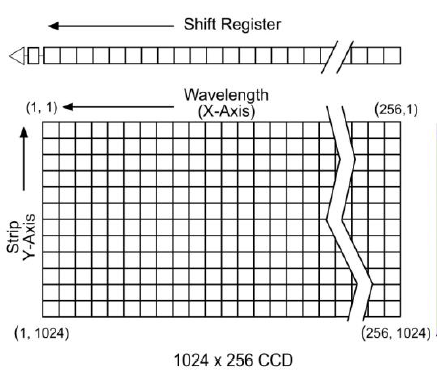
\includegraphics[width=0.5\textwidth]{pictures/1.PNG}
\caption{坐标轴定义。来自WinSpec User's Manual}
\end{figure}

\begin{itemize}
\item x1表示x轴选用的起始像素位置,x2表示x轴选用终止像素位置。y1,y2同理,表示y轴方向的像素选取。
\item x bin(binning),表示x轴每多少像素求和, y bin同理。为了增强信号,我们将y轴信号全部加起来,即 y bin 设置为 200。为了不降低分辨率,并没有对x轴信号进行部分求和,即 x bin 设置为1。
\end{itemize}
\textbf{WinSpec设置}: Acquisition>Experiment Setup
\begin{itemize}
\item Select Mode: Imaging Mode or Spectroscopy Mode
\item Clicking on \textbf{Full} loads the full size of the chip into the edit boxes.
\end{itemize}
\textbf{LightField设置}: Experiment Settings>Regions of Interest

\item 第三个子vi是示例vi: ExSubSetup.vi。This Sub VI sets up the skips, cleans, and shutter parameters. This should be changed to suit the camera you are using.由多个底层vi构成。
\begin{itemize}
\item 第一个底层vi:CameraCleans.vi。用来清除CCD芯片电荷的。
\\ \textbf{默认参数\footnote{这里默认参数指的是示例vi直接在后面板中设定好的参数}}:Number of Clears:1; Number of Strips Per Clear:50;  Continous Clears:0。
\\ \textbf{参数说明}:这部分参数说明要结合EMCDD说明书,参考其中Cleaning部分,这里摘抄如下。
\begin{itemize}
\item \emph{Number of Cleans} value is ususally set to one(1). These are additional clean cycles that can be required after a start exposure signal is received and the current clean cycle has finished. The maximum value for this entry depends on the camera.通常设为1。
\item \emph{Number of Strips per Clean} sets the number of rows that will be shifted 
and discarded per clean cycle. While a large number such as the number of rows in the array may result in the best cleaning of the array, the tradeoff is that there may be a significant delay between the receipt of a start exposure signal and the beginning of the actual exposure. This delay occurs because the current clean cycle must be completed before a start exposure signal received during the cycle will be implemented.Typically, the default setting is much smaller and in time critical experiments, the setting should be 1 or 2. 值越大清理的CCD行数越多,但是耗时也越多,需要用户权衡好。
\item \emph{Continuous Cleans} is available when the start of exposure is tied to an external trigger.This parameter is a flag that will allow clears to be performed "continuously" while running. This is the number o strips to clear before looking if an external trigger has arrived. This mode is usually used when collecting data with the camera in external trigger mode and the shutter disabled open.
\end{itemize}
\textbf{WinSpec设置}: Hardware Setup>Clean/Skips
\\ \textbf{LightField设置}: Experiment Settings>Sensor>Sensor Cleaning

\item 第二个底层vi:CameraShutter.vi。设置CCD的开和关。
\\\textbf{默认参数}:Shutter State:4;Shutter Compensation Time: Pre Open:0; Shutter Compensation Time: Post Open:0。
\\ \textbf{参数说明}:
\begin{itemize}
\item Shutter State设为4,表示CCD一直开着。
\item Shutter Compensation Time: Pre Open,只支持 Photometrics brand cameras 和 Acton InSpectrum camera,可以不连。
\item Shutter Compensation Time: Post Open的值必须设置,是CCD关闭的时间,单位是毫秒。
\end{itemize}
\textbf{WinSpec设置}:
\\ \textbf{LightField设置}: Experiment Settings>Shutter

\item 第三个底层vi:ToolKitIsError.vi。 检查SITK软件包是否有错误。
\end{itemize}

\item 第四个子vi是底层vi: CameraTrigger.vi。设置的是CCD信号触发模式。
\\ \textbf{默认参数}:Timing Mode:3(Strobed/Ext Sync);Trigger Edge:2。
\\ \textbf{参数说明}:
\begin{itemize}
\item Timing Mode:3表示选用的是外触发模式“Each exposure requires a trigger (Ext Sync, Strobed Mode)”;
\item Trigger Edge:2表示信号触发沿设定的是下降沿“Negative(falling) edge”。
\end{itemize}
\textbf{WinSpec设置}:
\\ \textbf{LightField设置}: Experiment Settings>Trigger>Readout Per Trigg

\item 第五个子vi是底层vi:CameraADCset.vi。 ADC,Analog to Digital Conversion,模拟信号转换为数字信号,模数转换。
\\ \textbf{默认参数}:ADC Speed:-2; ADC Gain:-1; Read Out port:-1; ADC offset:-1
\\ \textbf{参数说明}:
\begin{itemize}
\item ADC Speed: For Slowest ADC speed set this to -3; For Fastest ADC speed set this to -2; To use current ADC speed don't hook up or use -1 otherwise put speed in as KHz.
\item ADC Gain: To use current gain don't hook up or set to -1.
\item Read Out port: To use current readout port don't hook up or set to -1.
\item ADC offset: To use current offset don't hook up or set to -1.
\end{itemize}
\textbf{WinSpec设置}:
\\ \textbf{LightField设置}: Experiment Settings>Analog to Digital Conversion>Electron Multiplied

\item 第六个子vi是底层vi:CameraADCget.vi。获取当前模数转换的信息,示例vi中只输出了 ADC Speed 项。
\end{itemize}


(3)ExSetupExtSuperSyncro.vi:由一系列子vi构成,用来设置CCD的触发信号同步。
\begin{itemize}
\item 第一个子vi是示例vi: ExSubCheckCamPulser.vi。检查Camera和Pulser全局句柄是否创建。

\item 第二个子vi是示例vi: ExSubSetupCamPulserExtTrigSuperSync.vi。由一系列底层vi构成\footnote{注意:底层vi都是有详细说明文档的;底层vi中经常用到无符号长整型,但是用的时候可能用的有无符号长整型,虽然不会影响参数传递,但是在接口处有红点提示数据类型不是完全匹配}。
\begin{itemize}
\item 第一个底层vi是: CameraShutter.vi
\\ \textbf{与前面vi有重复,删除此处。}

\item 第二个底层vi是:CameraIntensMode.vi。设置光电倍增管的模式和强度。
\\ \textbf{参数}:Mode:2; Intensifier Gain: 20
\\ \textbf{参数说明}:
\begin{itemize}
\item Mode:2表示光电倍增管一直开着;
\item Intensifier Gain: 20表示增强值设为20。为什么是20不太清楚。
\end{itemize}
\textbf{WinSpec设置}:
\\ \textbf{LightField设置}: Experiment Settings>Analog to Digital Conversion>Electron Multiplied>EM Gain

\item 第三个底层vi是:CameraTrigger.vi
\\ \textbf{与前面vi有重复,删除此处。}


\item 第四个底层vi是:CameraCleans.vi
\\ \textbf{与前面vi有重复,删除此处。}

\item 第五个底层vi是:CameraSkips.vi
\\ \textbf{与前面vi有重复,删除此处。}

\item 第六个底层vi是:PulserExternalTrigger.vi。设置外触发模式以及相关参数。
\\ \textbf{参数}: Threshold:1; Slope:1; Coupling:1; Termination: 0
\\ \textbf{参数说明}: 
\begin{itemize}
\item Threshold:设置触发电压阈值,单位伏特(Volts)。
\item Slope:触发沿,0表示下降沿触发,表示上升沿触发。
\item Coupling:设置触发是交流(AC)触发还是直流(DC)触发,0表示ac,1表示dc。
\item Termination:设置阻抗,0表示50欧姆(Ohms),1表示高阻抗。
\end{itemize}
\textbf{Available only in Kinetics mode or DIF acquisition.}

\item 第七个底层vi是:PulserGateWidthDelay.vi。 This VI will set the gate width and delay values for repetitive pulsing in microseconds.
\\ \textbf{参数}: Gate Width: 0.1($\mu$s); Gate Delay: 0.0($\mu$s)
\\ \textbf{参数说明}:
\begin{itemize}
\item Gate Width: This value is the width of the gate pulse in microseconds.
\item Gate Delay: This value is the delay of the gate pulse in microseconds.
\end{itemize}

\item 第八个底层vi是:PulserOnChipAccum.vi。设置读取CCD芯片值前的曝光次数。
\\ \textbf{参数}: Accumulation:1
\\ \textbf{参数说明}:单脉冲测量关键,1表示曝光一次读取一次值,大于1表示曝光多次后读取一次值。

\item 第九个底层vi是:PulserSetVar.vi
\\ \textbf{默认参数}: Parameter ID:1002; Value:1601.0
\\ \textbf{参数说明}: Parameter ID,1002,表示Pulse Delay From;Value,1601.0表示 del from ext trig in, 而1602表示 del from t0 out.

\item 第十个底层vi是:PulserSetVar.vi
\\ \textbf{默认参数}: Parameter ID:1102; Value:0.0
\\ \textbf{参数说明}: Parameter ID,1102,表示Braket Pulse;Value,0.0表示 turn off braket pulse.
\end{itemize}
\end{itemize}


\section{PI-MAX3光谱采集LabVIEW程序解析}
CCD光谱采集LabVIEW程序是由示例程序 ExDataCollectPulserNframe.vi 改写过来的。这里详细说明下。
\begin{itemize}
\item 第一个子vi是示例vi: ExSubCheckCamPulser.vi。检查Camera和Pulser全局句柄是否创建。
\\ \textbf{初始化已经检查过了,这里删除?}

\item 第二个子vi是示例vi: ExSubInitCamPulser.vi。CCD初始化。由多个底层vi构成。
\begin{itemize}
\item 第一个底层vi是: CameraExperiment.vi。This function will allow the setup and running
of a basic data collection experiment. All advanced camera settings are set to good defaults.
\\ \textbf{参数}: Exposure(sec):0.0001(s,100$\mu$s); Number of Images: 200(\textbf{注:这里的严格表述应该为 Number of pulse})
\\ \textbf{默认参数}: Acquire/Focus Flag: 1; Number of Accumulations:1
\item 第二个底层vi是: PulserInit.vi。\textbf{什么是Pulser?}
\item 第三个底层vi是: CameraInitialzie.vi。初始化CCD,随时准备采集数据。
\end{itemize}

\item 第三个子vi是示例vi: ExSubCreateFileMultImage.vi由多个底层vi构成。
\\ \textbf{默认参数}:Number of Images:1。\textbf{和前面有重名需要进一步考察他们的功能。} 
\begin{itemize}
\item 第一个底层vi是: CameraGetDataDim.vi。This VI will return the X and Y dimension of one frame of data as defined in the camera.\textbf{不出意外,根据前面的设置,应该为1600*1,要测试下。}
\item 第二个底层vi是: ImageCreate.vi: This VI will create an image space to hold an image
of dimensions X and Y, number of frames and of the data type specified. A handle to this 
image is returned to provide access.
\\ \textbf{默认参数}: x dimension、y dimension:由前面vi获取得到;Data Type:4; Number of Frames: 1
\\ \textbf{参数说明}:
\begin{itemize}
\item X dimension: Number of data points in the X direction.
\item Y dimension: Number of data points in the Y direction.
\item Data Type: Type of binary representation of the data. 4=32-bit floating point
\item Number of Frames: Number of full frames of data X by Y in size.
\item Image Handle: A handle to image created is returned to provide access to the image. \textbf{Handle 到底是什么东西?}
\end{itemize}


\item 第三个底层vi是: FileOpen.vi。\textbf{并没有用到。}
\end{itemize}

\item 第四个子vi是示例vi:ExSubStartExpPulser.vi。由多个底层vi构成。
\begin{itemize}
\item 第一个底层vi是: PulserStart.vi
\item 第二个底层vi是: CameraStart.vi
\end{itemize}

\item 第五个子vi是示例vi: ExSubNframeColMultiImageFast.vi。由多个底层vi构成。
\\ \textbf{默认参数}:Number of Images:1。\textbf{和前面有重名需要进一步考察他们的功能。} 
\begin{itemize}
\item 第一个底层vi是: CameraCheckData.vi。This function will return the number of complete frames of data available to the calling function.
\item 第二个底层vi是: CameraGetData.vi。This VI will retrieve the data from the camera 
and store it in the data area of the data cluster parameter. The storage space for the
data must be pre-allocated by the caller. The dimensions to be allocated may be obtained
from the CameraGetDataDim VI.
\item 第三个底层vi是: ImageGetLineF32.vi。This VI will return a 1-dimensional line of data from an image in 32-bit Floating Point format. 
\\ \textbf{默认参数}: Y Position:1; Z Position:1
\\ \textbf{参数说明}:
\begin{itemize}
\item Data Handle: Handle to an image. This is obtained via the ImageCreate VI.
\item Z Position: This value is the 1-based position in the Z-axis of the frame of data from which the line of data is to be returned.
\item Y Position: This value is the 1-based position in the Y-axis of the line of data to be returned.
\end{itemize} 	
\end{itemize}

\item 第六个子vi是底层vi: ImageDestroy.vi

\item 第七个子vi是示例vi: ExSubStopCamPulser.vi。
\begin{itemize}
\item 第一个底层vi是: CameraStop.vi
\item 第二个底层vi是: PulserStop.vi
\end{itemize}
\end{itemize}















\part{Parallel computing}
参考资料
\begin{itemize}
\item  高性能计算之并行编程技术—— MPI并行程序设计
\end{itemize}
\chapter{背景知识}
\section{并行语言}
并行程序是通过并行语言来表达的,并行语言的产生主要有三种方式:
\begin{itemize}
\item 设计全新的并行语言\\
设计一种全新的并行语言的优点是可以完全摆脱串行语言的束缚, 从语言成分上直接支持并行。 这样就可以使并行程序的书写更方便, 更自然, 相应的并行程序也更容易在并行机上实现。 但是, 由于并行计算至今还没有象串行计算那样统一的冯•诺伊曼模型可供遵循,因此,并行机、并行模型、 并行算法和并行语言的设计和开发千差万别 ,没有一个统一的标准。虽然有多种多样全新的并行语言出现,但至今还没有任何一种新出现的并行语言, 成为普遍接受的标准。 设计全新的并行语言, 实现起来难度和工作量都很大。
\item 扩展原来的串行语言的语法成分使它支持并行特征\\
一种重要的对串行语言的扩充方式就是标注, 即将对串行语言的并行扩充作为原来串行语言的注释,对于这样的并行程序, 若用原来的串行编译器来编译, 标注的并行扩充部分将不起作用, 仍将该程序作为一般的串行程序处理, 若使用扩充后的并行编译器来编译, 则该并行编译器就会根据标注的要求, 将原来串行执行的部分转化为并行执行。对串行语言的并行扩充, 相对于设计全新的并行语言, 显然难度有所降低, 但需要重新开发编译器, 使它能够支持扩充的并行部分 。一般地, 这种新的编译器往往和运行时支持的并行库相结合。如openMP(Open Multi-Processing)。
\item 不改变串行语言 仅为串行语言提供可调用的并行库\\
仅仅提供并行库,是一种对原来的串行程序设计改动最小的并行化方法。 这样, 原来的串行编译器也能够使用 ,不需要任何修改 ,编程者只需要在原来的串行程序中加入对并行库的调用 就可以实现并行程序设计。MPI并行程序设计, 就属于这种方式。
\end{itemize}  
对于这三种并行语言的实现方法, 目前最常使用的是第二种和第三种方法 特别是第三
种方法。













\end{document}